% !TEX root = master.tex

\chapter{Dimensionality reduction algorithms}
\label{Ch:DimRedAl}
%\pagenumbering{arabic}

In this chapter dimensionality reduction algorithms which will be applied to solutions of the BGK model in Sod's shock tube are introduced: Proper orthogonal Decomposition (POD) and Autoencoders (AEs).\\
We will start off with a short introducing into POD, continue with autoencoders and finish with a detailed description of deep learning. Note that the main focus of this thesis lies in the application of autoencoders for which POD serves as a comparative method.\\
Dimensionality reduction algorithms lie at the heart of any reduced order model (ROM) which is described in the following chapter. As input serve datasets such as solutions of a full order model (FOM) or experimental data. These datasets may contain the dynamics of a spatio-temporal problem. The output is an approximation to the input. It is reconstructed from a low-dimensional representation that captured the underlying dynamics of the input problem. 
\section{Proper orthogonal decomposition (POD)}
\label{Sec: POD}
%POD
The solution of PDEs, precisely \(f(x,v,t)\), can be approximated either through a discretization into a system of ODEs as described in \cref{Ch:BGK}, or alternatively through a separation of variables ansatz
\begin{equation}
	f(t,v,x) = \sum_{i=1}^n a_i(t)\Phi_i(x,v)\mathrm{,}
\end{equation}  
as descried in \cite{Kutz}. Temporal dependence rendered through \(a_i(t)\) is independent from the spatial information carried in \(\Phi_i(x,v)\). Here \(\Phi_i(x,v)\) is called the \(i\)-th basis mode. With increasing \(i\), the accuracy of the solution consequently increases as well, which is similar to increasing the spatial resolution in finite difference methods outlined in \cref{Ch:BGK}. The essence of dimensionality reduction algorithms is now to find optimal basis modes \(\Phi_i(x,v)\). Optimality here means capturing the dynamic answer to a given geometry and inital conditions thus permitting to exploit a minimal number \(n\) of basis modes to reconstruct the dynamics.\\
An optimal basis can be provided by POD. It leverages a physically interpretable spatio-temporal decomposition of the input data \cite{Kutz}. At first this data needs to be preprocessed in a fashion, that seperates the temporal and spatial axis. Each temporal state is called snapshot and is stacked in a matrix \(\btch\) such that
\begin{equation}
	\btch=\left[ \mathbf{u}_{1},\mathbf{u}_2,\dots,\mathbf{u}_n \right] \qquad \mathrm{with}\qquad \mathbf{u}_i=\left[f(v_1,x_1),\dots,f(v_k,x_1),f(v_1,x_2),\dots,f(v_k,x_j)\right]^T \mathrm{,}
	\label{Eq:PiPOD}
\end{equation}
where \(n\) is the number of available snapshots and \(\mathbf{u}_i\) the \(i\)-th snapshot with \(\mathbf{u}_i \in \mathbb{R}^{j\times k}\). Afterwards \(\btch\) is decomposed using the singular value decomposition (SVD) which solves the left and right singular value problem leveraging
\begin{equation}
\btch = U\Sigma V^*\mathrm{,}
\end{equation}
where \(U\) is a unitary matrix containing the left singular vectors of \(\btch\) in it's columns and \(V\), also a unitary matrix, containing the right singular vectors in it's columns. Here superscribt asterix denotes the complex conjugate transpose. Furthermore \(\Sigma\) is a sparse matrix with the singular values in descending order on it's diagonal \cite{Kutz}. Note that the SVD always produces as much singular values and in turn singular vectors as there are elements on the shortest axis of the input matrix. Hence when preprocessing the input data as described above one gets as many singular values -and vectors as there are snapshots, given that the resolution in time is smaller than the spatial resolution.\\
Next, by applying the Eckard-Young theorem, that can be looked up in \cite{Kutz}, it is possible to solely harness the first leading singular values and corresponding vectors to approximate \(\btch\) to a desired accuracy. The theorem states that the the optimal rank-r approximation to $\btch$, in a least-squares sense, is given by the rank-r SVD truncation \(\tilde{\btch}\):
\begin{equation}
\underset{\tilde{\btch}, s.t. rank(\tilde{\btch})=r}{\operatorname{argmin}} \| 
\btch -\tilde{\btch}\|_F
=\tilde{U}\tilde{\Sigma}\tilde{V}^*\mathrm{.}
\label{Eq:EckardYoung}
\end{equation} 
Here \(\tilde{U}\) and \(\tilde{V}\) denote the first \(r\) leading columns of \(\mathbf{U}\) and \(\mathbf{V}\), and \(\tilde{\Sigma}\) contains the leading \(r \times r\) sub-block of \(\Sigma\). \(\|\cdot\|_F\) is the Frobenius norm \cite{Kutz}.\\
When decomposing a matrix that contains snapshots of a dynamical system, the columns of \(\tilde{U}\) and \(\tilde{V}\) contain dominant patterns that describe the dynamical system. Moreover they provide a hierarchical set of modes, that characterize the observed attractor on which we may project a low-dimensional dynamical system to obtain reduced order models. That being said, we use the left singular values of \(\tilde{U}\) as optimal basis modes such that
\begin{equation}
	\tilde{U} = \Phi = \left[\Phi_1,\Phi_2,\dots,\Phi_r\right]\mathrm{.}
\end{equation}
Vectors in \(\Phi\) are orthogonal to each other and in that way provide a coordinate transformation from the high dimensional input space onto the low dimensional pattern space.[PLS CHECK AGAIN, sentence is stolen from KUTZ]
\section{Autoencoders}
\label{Sec:AE}
%Autoencoder

Another way to obtain an optimal basis is to employ a machine learning architecture situated in the field of deep learning called autoencoders. An autoencoder is a feed forward neural network, that is trained to learn salient features of it's input by compressing it and successively reconstructing it back from the compressed version. In that way one could say that an autoencoder simply copies it's input to it's output \cite{Goodfellow}. \Cref{Fig:Autoencoder} shows a schematic representation of the architecture for a deep undercomplete autoencoder and the necessary terminology used to describe it's components. For the moment we ignore the difference between an undercomplete and overcomplete autoencoder, and come back to that when talking about regularization. \\
The biggest allocation unit in autoencoders is the distinction of a decoder and a encoder part, which are seperated at central code layer. The encoder is a mapping \(h\). The encoder maps the input \(\btch\) to the code \(\Phi\) while compressing it, which is written as \(h(\btch)=\Phi\). Hence the encoder consists of the input layer, a variable number of hidden layers and the code layer, which is the left side of the schematic autoencoder in \cref{Fig:Autoencoder}. The decoder mirrors the encoder, which is not a necessity but often chosen that way, see the right side of \cref{Fig:Autoencoder}. It comprises the same code layer, a variable number of hidden layers and the output layer. Similarily it is a mapping \(g\) which maps \(\Phi\) to \(\tilde{\btch}\), an approximation to the initial \(\btch\), and is written as \(g(\Phi)=\tilde{\btch}\). The number of hidden layers in encoder and decoder is the first of the so called hyperparameters that can be tuned to improve performance of the autoencoder. Note that we refer to autoencoders with more than one hidden layer, the code layer, as deep autoencoders. The reverse is a shallow autoencoder. The second largest allocation unit in autoencoders (and in general neural networks) are the layers. Each layer can be vector, a matrix or a three dimensional tensor. For the time beeing we choose each layer to be vector valued in the following. Therefore the input layer can be an input vector like \(\mathbf{u_1}\subseteq \btch\). The vectors in the hidden layers are abstractions of the input. The term hidden stems from the fact, that one usually does not look at them as the interest mainly lies in the code -and output layer. The code layer is of main interest, as is holds the compressed abstraction of the input. Coming to the smallest allocation unit, the nodes. Each node refers to an entry in the vector/layer and is dispalyed as a circle in \cref{Fig:Autoencoder}. The number of nodes per hidden layer is a second hyperparameter. Two nodes are connected in a forward pass through solving \(O=I*w+b\), which is represented as a computational graph in \cref{Fig:Autoencoder}. Here the input is \(I\), which is multiplied with a weight \(w\) and by adding a bias \(b\), one obtains the output \(O\). Hence every connection between nodes contains two free parameters: a weight \(w\) and a bias \(b\). Hence the whole network holds a set of parameters which we call \(\frepar \in \mathbb{R}\) in the following. A forward pass in this sense refers to the flow of information from the left side of the encoder to the right side of the decoder in \cref{Fig:Autoencoder}. All of the aforementioned can be found in \cite{Goodfellow}.\\
\begin{figure}
	\centering
	\begin{tikzpicture}

%input layer
\foreach \x [count=\y] in {0,.5,1.0,1.5,2,2.5}
	\node[circ] at (0,\x) (\y) {};
%hidden layer
\foreach \x  [count=\y from 7] in {0.25,0.75,1.25,1.75,2.25}
	\node[circ] at (2,\x) (\y) {};
%code layer
\foreach \x [count=\y from 12] in {0.75,1.25,1.75}
\node[circ] at (4, \x) (\y) {};
%hidden layer
\foreach \x  [count=\y from 15] in {0.25,0.75,1.25,1.75,2.25}
\node[circ] at (6,\x) (\y) {};
%output layer
\foreach \x [count=\y from 20] in {0,.5,1.0,1.5,2,2.5}
\node[circ] at (8, \x)   (\y) {};
\begin{pgfonlayer}{background}
%draw connections
\foreach \x in {1,...,6}
\foreach \y in {7,...,11}
	\draw (\x) -- (\y);
\foreach \x in {7,...,11}
\foreach \y in {12,...,14}
\draw (\x) -- (\y);
\foreach \y in {12,...,14}
\foreach \x in {15,...,19}
\draw (\x) -- (\y);
\foreach \y in {15,...,19}
\foreach \x in {20,...,25}
\draw (\x) -- (\y);
\end{pgfonlayer}
%dots
\path (3,0)--(3,2.5) node[ellipse,rotate=90,midway, fill=white] {\vdots\hspace{0.5em} \vdots\hspace{0.5em} \vdots \hspace{0.5em} \vdots};
%dots
\path (5,0)--(5,2.5) node[ellipse,rotate=270,midway, fill=white] {\vdots\hspace{0.5em} \vdots\hspace{0.5em} \vdots \hspace{0.5em} \vdots};

%\draw [thick,decorate,decoration={brace,mirror,amplitude=5pt}] (-.3,-.5) -- (1.98,-.5) node [midway,below = 8pt,draw=none,rectangle split,rectangle split parts=2] 
%{Encoder:\nodepart{second} \(h(\Pi)=\Phi\)};
%\draw [thick,decorate,decoration={brace,mirror,amplitude=5pt}] (2.02,-.5) -- (4.3,-.5) node [ midway,below= 8pt,draw=none,rectangle split,rectangle split parts=2] {Decoder: \nodepart{second} g(\Phi)=$\tilde{\Pi}$};
%\draw [thick,decorate,decoration={brace,amplitude=3pt}] (-.3,2.75) -- (.3,2.75) node [midway,above = 8pt,draw=none,rectangle split,rectangle split parts=2] 
%{Input \nodepart{second}Layer};
%\draw [thick,decorate,decoration={brace,amplitude=3pt}] (1.7,2) -- (2.3,2) node [midway,above = 8pt,draw=none,rectangle split,rectangle split parts=2] 
%{Hidden \nodepart{second}Layer};
%\draw [thick,decorate,decoration={brace,amplitude=3pt}] (3.7,2.75) -- (4.3,2.75) node [midway,above = 8pt,draw=none,rectangle split,rectangle split parts=2] 
%{Output \nodepart{second}Layer};
\end{tikzpicture}

	\caption{\footnotesize Scheme of an undercomplete autoencoder with five fully connected layers. Input layer, output layer, the code or bottleneck layer and two hidden layers. Every layer is made up of nodes, which are represented as circles. The more hidden layers are added to the architecture the deeper is the autoencoder and the greater the capacity of the model. Not shown are possible activations for each layer. Labelled is decoder and encoder. The decoder is a mapping \(g(\Phi)=\tilde{\btch}\), taking \(\Phi\) as input and outputs an approximation \(\tilde{\btch}\) of \(\btch\). Similarily the encoder is a mapping \(h(\btch)=\Phi\), taking \(\Phi\) as input and outputs the code \(\Phi\). The box left of the autoencoder shows a computational graph for the feed forward connection of two nodes. The input of a node is \(I\) which is multiplied with \(w\) a weight. A bias \(b\) is added to the result \(I^*\) which yields the output \(O\), input of a node right of the inital node.}
	\label{Fig:Autoencoder}
\end{figure}
\subsection{Training}
%Training

In a feed forward neural network, as the autoencoder used in this thesis, the information flows forward from input to output layer when we want to perform an evaluation as in \(AE(\btch) = g(h(\btch)) =\tilde{\btch }\). In that way the layer structure in \cref{Fig:Autoencoder} can be viewed as evaluating a composition of functions
\begin{equation}
	l^{(4)}(l^{(3)}(l^{(2)}(l^{(1)}(l^{(0)}(\btch))))) = g(h(\btch)) = AE(\btch) = \tilde{\btch}\mathrm{,}
	\label{Eq:Composition}
\end{equation}
where every function represents one layer. Here \(l_{(0)}\) and \(l_{(4)}\) are input layer and output layer, \(l_{(1)}\) and \(l_{(3)}\) the hidden layers in encoder and decoder with \(l_{(2)}\) the bottleneck layer. The evaluation of one layer or function is a linear transformation of the incoming data with
\begin{equation}
\tilde{\mathbf{u}}_1 = \mathbf{u}_1W + \mathbf{b}\mathrm{.} \label{Eq:Linear Transformation}
\end{equation}
Here \(\mathbf{u}_1\) is as in \cref{Eq:PiPOD}, \(W\) is the weight matrix and \(\mathbf{b}\) a bias vector, which is the same equation as shown in the computational graph in \cref{Fig:Autoencoder}. The weight matrices and bias vectors of each layer are collected in the set \(\frepar \in \mathbb{R}\).  It is self evident, that \(\frepar\) does not minimize the cost function \(J(\frepar)\) from the start with
\begin{equation}
	J(\frepar) := \frac{1}{n}\sum_{i=1}^n (\mathbf{u}_i - AE(\frepar;\mathbf{u}_i))^2\mathrm{,}
	\label{Eq:Cost}
\end{equation}
and needs to be found through a learning process, which is called training. The training will be discussed in the following.\\
Note that the cost function \(J(\theta)\) comprises the mean squared error over all snapshots \(\mathbf{u}_i\), which we will write as \(L(\btch,\tilde{\btch})\) the so called loss with
\begin{equation}
	L(\btch,\tilde{\btch}) := \frac{1}{n}\sum_{i=1}^n(\mathbf{u}_i - \tilde{\mathbf{u}}_i)^2 = E \mathrm{,}
\end{equation}
when specifically referring to \(E\) the distance between \(\btch\) and $\tilde{\btch}$. In order to minimize \(J(\frepar)\) we compute the gradient of \(J(\frepar)\) with respect to the free parameters \(\frepar\) written as \(\nabla_{\frepar}J\). Specifically we need to compute the derivative of the network with respect to the free parameters as seen in \cref{Eq:Cost}. Then we move in the opposite direction of the gradient, which yields an update of \(\frepar\) as
\begin{equation}
	\frepar \leftarrow \frepar - \epsilon\grd\mathrm{,} \qquad\mathrm{where}\qquad \grd:= \nabla_{\frepar}J\mathrm{.}
	\label{Eq: update}
\end{equation}
\begin{wrapfigure}{r}{.2\textwidth}
	\centering
	\vspace{-10pt}
	\begin{tikzpicture}
%\tikzstyle{every node} = [font=\footnotesize]
	\node [circ] (x) {\(x\)};
	\node [circ,above of = x] (z) {\(z\)};
	\node [circ,above of = z] (y) {\(y\)};
	\draw [arrow] (x)--(z) node [midway,xshift=1ex] {f};
	\draw [arrow] (z)--(y) node [midway,xshift=1ex] {g};
\end{tikzpicture}
	\vspace{-5pt}
	\caption{\footnotesize A single node network with one hidden node between input and output node.}
	\label{Fig:Sing_example}
\end{wrapfigure}
\textbf{Backpropagation:} The computation of the gradient \(\grd\) is done in the so called backpropagation. As the name implies the information flows backwards through the network, from output to input layer, and propagates \(E\) backwards through the network. Responsible for this backward motion is the recursive application of the chain rule of calculus. Considering as a simple illustrative example \cref{Fig:Sing_example} with \(y=g(z,b)=g(f(x,a))\), a single node connection from input \(x\) to output \(y\) with a single hidden node. Then \(a\) is a weighting constant of the first node and \(b\) defines a weighting consant of the hidden node. Backpropagating the distance \(E\) with \(E = \frac{1}{2}(y_0 -y)^2\) between the output and the ground truth \(y_0\) though the network yields
\begin{align}
	\frac{\partial E}{\partial a} &= -(y_0 - y)\frac{\partial y}{\partial z}\frac{\partial z}{\partial a}\qquad \mathrm{and}\\
	\frac{\partial E}{\partial b} &= -(y_0 - y)\frac{\partial y}{\partial b}\mathrm{,}
\end{align}
which requires \(\frac{\partial E}{\partial a} = -(y_0 - y)\frac{\partial y}{\partial z}\frac{\partial z}{\partial a} = 0\) to minimize \(E\). The update rule is then given by
\begin{equation}
	a_{i+1} = a_i + \epsilon \frac{\partial E}{\partial a_i} \qquad\mathrm{and}\qquad
	b_{i+1} = b_i + \epsilon \frac{\partial E}{\partial b_i}\mathrm{.}
\end{equation}
This example is taken from \cite{Kutz} and shows the manner in which the chain rule of calculus provides the backwards direction when deriving the gradients of each layer with respect to the free parameters.\\
\textbf{Generalization:}
At this point the objective for training a neural network is specified. The difference between pure optimization and learning lies in their differing objectives. In pure optimization a cost function like \(J(\frepar)\) is minimized in order to fit \(\btch\) to \(\tilde{\btch}\). This is called the objective of the optimization task. Learning on the other hand uses the same objective as the optimization task, but equally cares about the so called generalization task. In machine learning generalization refers to the ability of the learning algorithm to not only fit the input data, but also to fit data it has not seen before. It does so by using salient features of the input data which enables generalization. This can only be achieved to a certain extend and is sometimes intractable. But how is the generalizing performance measured? We randomly shuffle the input data \(\btch\) and split it into a training and a validation set in a 80/20 fashion with \(\btch=\{\btch_{train},\btch_{val}\}\). The random shuffling is performed as to eliminate any bias on both sets. Then we minimize \(J(\frepar)\) using only \(\btch_{train}\) which minimizes \(L(\btch_{train},\tilde{\btch}_{train})\) and check if indirectly \(L(\btch_{val},\tilde{\btch}_{val})\) is beeing minimized as well. The indirect minimization of \(L(\btch_{val},\tilde{\btch}_{val})\) is called the generalization task. The loss over the validation set is called the validation error and the loss over the training set is called the train error. Note that in learning both tasks are equally valued. As mentioned before, we want to learn an optimal basis \(\base\) which specifically contains salient features of \(\btch\). With minimizing only the optimization task, we acquire the same basis as in POD. With learning we try to find an even more powerful basis \(\base\) that enables the network to generalize.\\ 
\textbf{Adam:}
The algorithm to compute the updates to \(\frepar\) is called Adam, an upgraded version of the classic stochastic gradient descent algorithm (SGD) with moments. The name stems from adaptive moment estimation, which refers to the adaptation of moments which in combination with the learning rate \(\epsilon\) apply scaled, directional updates to \(\frepar\) during training. Moments and how they are adapted are discussed a bit further on. The steps of Adam are shown in \cref{Alg:Adam} and explained successively. There we initially define hyperparameters which are the step size/learning rate \(\epsilon\), exponential decay rates \(d_1\) and \(d_2\) in \([0,1)\) and a small constant \(\delta\) for numerical stability. We can use the default values for all constants with \(\epsilon=1e-2\), \(d_1=0.9\), \(d_2=0.999\) and \(\delta=1e-8\).  Despite the learning rate \(\epsilon\), Adam is fairly robust w.r.t. changing it's hyperparameters. Hence solely the hyperparameter \(\epsilon\) requires tuning.
\begin{algorithm}[hbp!]
	\begin{algorithmic}
		\SetAlgoLined
		\REQUIRE Step size $\epsilon$
		\REQUIRE Exponential decay rates from moment estimates $d_1$ and $d_2$ in \([0,1)\)\\
		(Suggested defaults: 0.9 and 0.999 respectively)
		\REQUIRE Small constant $\delta$ used for numerial stabilization (Suggested default: $10^{-8}$)
		\REQUIRE Initial parameters $\frepar$\\
		Initialize 1st and 2nd moment variables \(\mathbf{s}=0\) and \(\mathbf{r}=0\)\;
		Initialize time step i = 0\;
		\While{stopping criterion not met}{
			Sample a minibatch $\minib_i$ containing  \(m\) examples from the training set \(\btch_{train}\)\;
			Compute gradient: \(\grd\ \leftarrow \frac{1}{m} \nabla_{\frepar} \sum_m L(\minib_i - AE(\frepar;\minib_i)\)\;
			\(t\leftarrow t + 1\)\;
			Update biased first moment estimate: $\mathbf{s} \leftarrow d_1\mathbf{s} + (1-d_1)\grd$\;
			Update biased second moment estimate: $\mathbf{r} \leftarrow d_2\mathbf{r} + (1-d_2) \grd\circ\grd$\;
			Correct bias in first moment: $\hat{\mathbf{s}} \leftarrow \frac{\mathbf{s}}{1-d_1^i}$\;
			Correct bias in second moment: $\hat{\mathbf{r}} \leftarrow \frac{\mathbf{r}}{1-d_2^i}$\;
			Compute update: $\Delta\frepar = -\epsilon \frac{\hat{\mathbf{s}}}{\sqrt{\hat{\mathbf{r}}}+\delta}$ (operations applied element-wise)\;
			Apply update: $\frepar \leftarrow \frepar + \Delta\frepar$
		}
	\end{algorithmic}
	\caption{The Adam algorithm}
	\label{Alg:Adam}
\end{algorithm} 
Next we initialize the 1st and 2nd moments \(\mathbf{s}\) and \(\mathbf{r}\) to zero, in contrast to \(\frepar\), which is initialized as follows.\\
The selection of starting values for \(\frepar\) is of crucial importance for the success of any neural network to learn something useful in a reasonable time. Moreover it strongly affects if the learning algorithm converges at all. This is partly because with the starting point we introduce a strong bias on the network considering that the SGD algorithm only makes marginal contributions to \(\frepar\) at every update. Even if \(J(\frepar)\) reaches a minimum, different initial values can lead to a variety of generalization errors. Specifically this connection between initial parameters and generalization is not well understood. Note that the topic of parameter initialization is despite it's importance, only sketched out briefly in this thesis. For more details see \cite{Goodfellow} for an overview, \cite{LeCun98} for the default initialization in \texttt{pytorch}, which is also used in this thesis and \cite{he2015} for very deep networks with more than eight layers and rectifying non-linear activations.\\
Usually the biases can be chosen to a heuristically constant value, while the weights need to be initialized so that they break symmetry between nodes. Imagine two hidden nodes with the same activation function connected to the same input. The same gradient would lead to a symmetric evolution during training, making one of the nodes redundant. Hence weights are initialized randomly often drawn from a Gaussian distribution. Next, finding the right scale for the distribution, which in turn scales the initial weights, is tackled. The spectrum of initial weight sizes ranges from large initial weights which are beneficial for breaking any symmetry, to small initial weights or even a sparse initialization. Now with this in mind, if we scale the distribution to produce large weights, we induce a prior, which states that all nodes are connected and how they are connected. Small initial weights on the other hand induce a prior, that says that it is more likely for nodes to not be connected and that the learning algorithm can choose which nodes to connect and how strong.\\
There exist several heuristics for the scale of the initial weights, which try to preserve the norm of the weigh matrix of each layer, to stay close to or below unity. Envisage that during forward as well as backward propagation we perform matrix multiplications from one layer to the next. Keeping the norm of each layer from exceeding unity, we prevent the development of exploding values and gradients in the respective last layer. A preventive measure is to scale the distribution for one layer with respect to it's non-linear activation with a factor called gain. Gains for non-linear activations can be found in \cite{torch_ini} along with several sampling methods. The effects described above become severe with large layers or equally with networks of a certain depth, which is not the case for the autoencoders used in this thesis allowing to comfortably choose the default initialization in \texttt{pytorch} for linear -and convolutional layers where we draw the initial weights from a normal distribution with \(U(-\frac{1}{\sqrt{m}},\frac{1}{\sqrt{m}})\) as suggested in \cite{LeCun98}. The number of input nodes, also called fan-in, per layer is \(m\).\\
SGD is derived from the common gradient decent method, where the whole batch \(\btch_{train}\) is used per iteration to compute the gradient for an update of \(\frepar\) in the opposite direction of the gradient. Hence gradient descent is a so called batch gradient method or deterministic gradient method. SGD is a stochastic method. It approaches updates for \(\frepar\) as in \cref{Eq: update} in a stochastic manner, using only small portions of \(\btch_{train}\) per update. By randomly sampling only a small number of examples from \(\btch_{train}\) and taking the average gradient over those examples we compute an estimate of the true gradient which is much cheaper. Therefore SGD trains with so called minibatches of a certain size, which yields \(\btch_{train} = \{\btch_{t_i},\dots,\btch_{t_n}\}\). Here \(i\) counts through all the minibatches and \(n\) is the total number of minibatches. The size of one minibatch can be obtained through dividing the dimension of your input, on which you split the batch, by \(n\) and is called \(\mbs\) in the following and is another hyperparameter. Minibatch sizes \(\mbs\) are influenced by the following observations. As one minibatch can be processed in parallel to compute an update, extremely small \(\mbs\) underutilize multicore architectures. Extremely large \(\mbs\) on the other hand can be limited by available memory to be solved in parallel. When utilizing a graphics processing unit (GPU) \(\mbs\) of the power of two is advised to fully exhaust the whole hardware (array sizes of the power of two achieve better runtime in GPUs). Small \(\mbs\) can have a regularizing effect hence improve generalization, but also amplify the noisy behavior \cite{Goodfellow}[p.270ff].\\
Stochasticity is key in SDG and is achieved by shuffling the input data, which was already performed for the training and validation split. On every update the gradient is evaluated as an average over a minibatch of randomly sampled examples, yielding an unbiased estimate of the true gradient. This measure leads to noisy updates of \(\frepar\) which improves generalization and converges faster than common gradient descent. SGD has the ability to find a minimum even before the whole batch is processed, especially with large datasets, as elaborated in \cite{Goodfellow}[p.286 ff]. 
The noisy updates require a small learning rate, especially when the the minibatch size  \(\mbs\) is small, that decays over time as the noise does not vanish when a minimum is found. Up to now we saw that small minibatches improve generalization, underutilize available multicore hardware and amplify noisiness which needs to be tackled with small learning rates. Therefore the learning process is slowed down. Here momentum comes into play, which accelerates learning.\\
Momentum applies an exponentially decaying moving average of previous gradients to the current gradient. Momentum is an analogy to momentum in physics and therefore named after. Imagine a tightrope walker, who uses the moment of inertia of a long rod for balance as crossing the rope. Oscillations of the walker need to overcome the moment of inertia of the long rod in order to destabilize the walker. Another analogy is a fast car taking a sharp turn. The car drifts because the new direction is influenced by the old orthogonal momentum. If we take the update rule for the first moment estimate \(\mathbf{s}\) of \cref{Alg:Adam} and look at three consecutive updates
\begin{align}
	\mathbf{s}_i &= d_1\mathbf{s}_{i-1}+(1-d_1)\mathbf{g}_{i}\mathrm{,} \label{Eq: fm}\\
	\mathbf{s}_{i-1}&=d_1\mathbf{s}_{i-2}+(1-d_1)\mathbf{g}_{i-2}\mathrm{,}\\
	\mathbf{s}_{i-2}&=d_1\mathbf{s}_{i-3}+(1-d_1)\mathbf{g}_{i-3}\mathrm{,}
\end{align}
we see that by combining and simplifying the three updates yields
\begin{equation}
	\mathbf{s}_i = d_1d_1(1-d_1)\mathbf{g}_{i-2}+\dots+d_1(1-d_1)\mathbf{g}_{i-1}+\dots+(1-d_1)\mathbf{g}\mathrm{.}
\end{equation}
Note that this entanglement of the updates is taken from \cite{bushaev_2017}. Obviously the contributions to the current gradient vanish exponentially over iterations. This leads to a moving average of past and current gradients. Now taking into account that if \cref{Eq: fm} computes the moment of the first iteration, there are no previous gradients available which leads to a biased first computation. Hence we divide \(\mathbf{s}_i\) by \((1-d_1^i)\) for the bias correction of the first moment in \cref{Alg:Adam} which yields \(\hat{\mathbf{s}}\). In consecutive iterations obviously the bias correction approaches zero. All the same steps does the second biased moment estimate \(\mathbf{r}\) take. The second moment estimate is nothing more than the squared past gradients gradients written as \(\grd \circ\grd\) in \cref{Alg:Adam}. Together they from the parameter update \(\Delta\frepar\). Without going into further details, it can be shown that the parameter updates have an approximate upper bound of \(\Delta\frepar\lessapprox \epsilon\), see \cite{kingma2017adam}. This upper bound is a necessary criteria for the updates, as the learning rate \(\epsilon\) is a specifically tuned hyperparameter that should not be exceeded during training. The ratio \(\frac{\hat{\mathbf{s}}}{\sqrt{\hat{\mathbf{r}}}+\delta}\) is called signal to noise ratio (SNR) in \cite{kingma2017adam}, which evolves towards zero as an optimum is reached. Furthermore, the updates are invariant to the scale of the gradients as a factor \(a\) is always canceled out with \((a\cdot\hat{\mathbf{s}})/\sqrt{(a^2\cdot\hat{\mathbf{r}})}=\hat{\mathbf{s}}/\sqrt{\hat{\mathbf{r}}}\). To sum up, using first and second momentum we can accelerate training as the moving average gradient smooths the noisy updates and in turn is a better estimate of the true gradient, the bias in the first iteration is corrected and we stay invariant to gradient scaling.\\       
\begin{figure}[htbp!]
	\centering
	%flowchart training
\begin{tikzpicture}[%
>=triangle 60,              % Nice arrows; your taste may be different
start chain=going below,    % General flow is top-to-bottom
node distance=6mm and 60mm, % Global setup of box spacing
every join/.style={norm},   % Default linetype for connecting boxes
]
% ---------
\tikzset{
	base/.style={draw, on chain, on grid, align=center, minimum height=4ex},
	proc/.style={base, rectangle, text width=12em},
	test/.style={base, diamond, aspect=2, text width=5em},
	term/.style={proc, rounded corners,text width = 8em},
	% coord node style is used for placing corners of connecting lines
	coord/.style={coordinate, on chain, on grid, node distance=6mm and 25mm},
	% nmark node style is used for coordinate debugging marks
	nmark/.style={ draw=none,color0, on chain, on grid, node distance=6mm and 25mm},
	% -------------------------------------------------
	% Connector line styles for different parts of the diagram
	norm/.style={->, draw},
	it/.style={font={\small\itshape}}
}
\tikzstyle{every node} = [font=\footnotesize]
	% Start by placing the nodes
	\node [proc] (mb) {Partition \(\btch_{train}\) into \(n\) Minibatches:\\ \(\btch_{train} = \{\minib_{i},\dots,\minib_{n}\}\)};
	\node [proc,join] (E0B0) {Epoch counter: \(E_i = 0\)\\Batch counter: \(B_i=0\)};
	\node [proc,join] (ini) {Initialize weights};
	\node [test,join] (t1) {\(E_i \leq E_{H}\)};
	\node [test,join] (t2) {\(B_i\leq B_{n}\)};
	\node [proc,join] (p1) {Evaluate:\\ \(AE(\minib_i)=\tilde{\minib}_i\)};
	\node [proc,join] (p2) {Evaluate:\\ \(L(\minib_i,\tilde{\minib}_i)=E_i\)};
	\node [proc,join] (p3) {Backpropagate\\ \(E_i\)};
	\node [proc,join] (p4) {Optimize \(w\) and \(b\):\\\(Adam(w_n,b_n)=(w_{n+1},b_{n+1})\)};
	\node [proc,join] (Bplus) {\(B_{i+1} = B_i + 1\)};
	%side nodes	
	\node [proc,right =of mb] (tv) {Partition \(\btch\) into training and validation set:\\ \(\btch = \{\btch_{train},\btch_{val}\}\)};
	\node [proc, right=of t2] (p5) {Evaluate:\\ \(AE(\btch_{val})=\tilde{\btch}_{val}\)};
	\node [proc, right=of p1,join] (p6) {Evaluate:\\ \(L(\btch_{val},\tilde{\btch}_{val})=E_{val}\)};
	\node [proc, right=of p2,join] (aveMSE) {\(\frac{1}{N} \sum_n E_{B_n} =\overline{E}_B\)} ;
	\node [proc, right=of p3,join] (Eplus) {\(E_{i+1} =E_i + 1\)} ;
    \node [term,left=of t1] (fini) {finish};

    \node [coord, left=of Bplus,xshift=-2em]  (c4)  {};
    \node [coord, right=of Eplus,xshift=2em]   (c5)  {};
    %connections
    \draw [->] (tv) -- (mb);
	\draw [->] (t1.west) -- (fini); 
	\draw [->] (t2.east) -- (p5);
	\draw [->] (Eplus.east) -- (c5)|-(t1); 
	\draw [->] (Bplus.west) -- (c4)|-(t2); 
	%decisions
	\path (t1.south) to node [near start, xshift=1em] {$y$} (t2);
	\path (t1.west) to node [near start, yshift=1em] {$n$} (fini);
	\path (t2.south) to node [near start, xshift=1em] {$y$} (p1);
	\path (t2.east) to node [near start, yshift=1em] {$n$} (p5);
	%labels
	\node [nmark,right =of tv,xshift=1em]  {(a)}; 
	\node [nmark,left =of mb,xshift=-1em]  {(b)}; 
	\node [nmark,right =of ini,xshift=1em] {(c)}; 
	\node [nmark,right =of p1,xshift=1em]  {(d)};
	\node [nmark,right =of p2,xshift=1em]  {(e)};
	\node [nmark,right =of p3,xshift=1em]  {(f)};
	\node [nmark,right =of p4,xshift=1em]  {(g)};
	\node [nmark,right =of p5,xshift=1em]  {(h)};
	\node [nmark,right =of p6,xshift=1em]  {(i)};
	\node [nmark,right =of aveMSE,xshift=1em]  {(j)};
\end{tikzpicture}
	\caption{\footnotesize Flowchart of the training process used in this thesis for an autoencoder. The data set \(\btch\) for training is split up into a training \(\btch_{train}\) and a validation \(\btch_{val}\) set with a \(80/20\) ratio (a). The \(\btch_{train}\) set is equally devided into \(n\) minibatches (b). The network will be trained over \(H\) epochs and \(n\) minibatches. First the weights \(w\) are initialized as in \cite{LeCun98} and biases set to zero (c). A successive evaluation of the first minibatch with \(AE(\minib_{i})=\tilde{\minib}_{i}\) called forward propagation takes place in (d). The mean squared error between \(\minib_{i}\) and \(\tilde{\minib}_{i}\) yields the average error over one minibatch \(E_{B_i}\). Thereafter \(E_{B_i}\) is backpropagated through the network (f) yielding the gradient \(\grd\). This gradient is then used to optimize weights \(w\) and biases \(b\) with  \(Adam\), an optimization algorithm seen in \cref{Alg:Adam}, (g). In the fashion of using (d) to (g) all \(n\) minibatches are shown to the network and lead to an optimization of the network's free parameters \(\frepar\) which are weights \(w\) and biases \(b\). After all minibatches are shown to the network a validation step is taken. Hence the network evaluates \(\btch_{val}\), which it has not seen before, in (h) with \(AE(\btch_{val})=\tilde{\btch}_{val}\). Subsequently, the evaluation of the mean squared error between \(\btch_{val}\) and \(\tilde{\btch}_{val}\), produces the validation error \(E_{val}\) in (i). Afterwards the arithemtric mean of all minibatch errors \(E_{B_i}\) is taken. This produces \(\overline{E}_B\) and concludes the first epoch. The maximum number of epochs \(H\) is reached when \(E_B\) and \(E_{val}\), have dropped to a satisfactory value and the training finishes.}
	\label{Fig:Training}
\end{figure}\noindent
The flowchart in \cref{Fig:Training} shows how the generalization query, weight initialization, backpropagation and the integration of Adam into the training procedure is carried out within this thesis. The network is trained in two loops, where the outer runs over so called epochs and the inner over all minibatches. One epoch is completed after all minibatches are shown to the network and the validation error is calculated as well as the train error, for which we take the average over all minibatches. The number of epochs \(H\) is determined based on over- and underfitting as well as on how many epochs are needed for Adam to converge and is another hyperparameter. In the following capacity, regularization, over- and underfitting is described.\\
\begin{figure}[htbp!]
	\centering
	% This file was created by tikzplotlib v0.9.6.
\pgfplotsset{
	set layers,% using layers
	mark layer=axis tick labels% defines the layer of the marks
}
\begin{tikzpicture}
\begin{axis}[
tick align=outside,
tick pos=left,
x grid style={white!69.0196078431373!black},
xlabel={\LARGE Capacity},
xmin=0, xmax=10.4915254237288,
xticklabels = {0,\LARGE Optimal capacity},
xtick={0,3.2},
y grid style={white!69.0196078431373!black},
ylabel={\LARGE Error},
ymin=-0.501805191944399, ymax=12.7389078292872,
ytick=\empty,
ytick style={color=black},
yticklabels = {,,},
width=2\textwidth,
height=1.3\textwidth,
x label style={yshift=.5em},
]
\addplot [thick, black , mark=o, mark size=2, mark options={solid}]
table {%
	0 inf
	0.169491525423729 12.137057237413
	0.338983050847458 8.21466201662695
	0.508474576271186 6.41053580146569
	0.677966101694915 5.22604286369211
	0.847457627118644 4.34623242909512
	1.01694915254237 3.65593083737413
	1.1864406779661 3.09878041398807
	1.35593220338983 2.64171108959936
	1.52542372881356 2.26288853542921
	1.69491525423729 1.94673997609849
	1.86440677966102 1.68157958464115
	2.03389830508475 1.45833647170967
	2.20338983050847 1.26980624712581
	2.3728813559322 1.12866830116967
	2.54237288135593 1.04045080409685
	2.71186440677966 0.971417809099685
	2.88135593220339 0.919088748511067
	3.05084745762712 0.881388366601579
	3.22033898305085 0.856583391159462
	3.38983050847458 0.843229082204998
	3.5593220338983 0.840124118103997
	3.72881355932203 0.846272519273589
	3.89830508474576 0.860851512240569
	4.06779661016949 0.88318440782768
	4.23728813559322 0.912717711615713
	4.40677966101695 0.949001806706436
	4.57627118644068 0.991674651695909
	4.74576271186441 1.04044802361793
	4.91525423728813 1.09509590893097
	5.08474576271186 1.15544470750812
	5.25423728813559 1.22136496682895
	5.42372881355932 1.29276440766818
	5.59322033898305 1.36958203979763
	5.76271186440678 1.45178319763694
	5.93220338983051 1.53935535230884
	6.10169491525424 1.63230457894079
	6.27118644067797 1.73065257694982
	6.44067796610169 1.83443415699726
	6.61016949152542 1.9436951217619
	6.77966101694915 2.05849047904398
	6.94915254237288 2.17888293530334
	7.11864406779661 2.30494162583108
	7.28813559322034 2.43674104458708
	7.45762711864407 2.57436014250381
	7.6271186440678 2.71788156792447
	7.79661016949153 2.86739102695298
	7.96610169491525 3.02297674496113
	8.13559322033898 3.18472901342541
	8.30508474576271 3.35273980873682
	8.47457627118644 3.52710247171199
	8.64406779661017 3.70791143829411
	8.8135593220339 3.89526201341727
	8.98305084745763 4.08925018126187
	9.15254237288136 4.28997244618645
	9.32203389830508 4.49752569951442
	9.49152542372881 4.71200710810794
	9.66101694915254 4.93351402129678
	9.83050847457627 5.16214389326735
	10 5.39799421846945
};
\addlegendentry{\LARGE Validation error}
\addplot [thick, color0, mark=+, mark size=2, mark options={solid}]
table {%
0 inf
0.169491525423729 6.74409390778825
0.338983050847458 3.66249452516524
0.508474576271186 2.56807895469113
0.677966101694915 1.98264844839045
0.847457627118644 1.60850296258454
1.01694915254237 1.34503007352016
1.1864406779661 1.14816315771571
1.35593220338983 0.995206947153229
1.52542372881356 0.873084419642305
1.69491525423729 0.773614788943724
1.86440677966102 0.69135176109086
2.03389830508475 0.622491198528442
2.20338983050847 0.564274344179929
2.3728813559322 0.514640334137393
2.54237288135593 0.472012814370054
2.71186440677966 0.435162870611037
2.88135593220339 0.403117523010918
3.05084745762712 0.375096584488649
3.22033898305085 0.35046783225793
3.38983050847458 0.328714390718848
3.5593220338983 0.309410492762954
3.72881355932203 0.29220313698828
3.89830508474576 0.276797987992008
4.06779661016949 0.262948391470186
4.23728813559322 0.250446716304759
4.40677966101695 0.239117462143469
4.57627118644068 0.228811724792275
4.74576271186441 0.219402718421571
4.91525423728813 0.210782128978517
5.08474576271186 0.202857127402874
5.25423728813559 0.195547910838997
5.42372881355932 0.188785669382798
5.59322033898305 0.182510897943167
5.76271186440678 0.176671989552264
5.93220338983051 0.171224059336657
6.10169491525424 0.16612795835743
6.27118644067797 0.161349444356969
6.44067796610169 0.156858482632537
6.61016949152542 0.152628655174172
6.77966101694915 0.148636660141543
6.94915254237288 0.144861886925093
7.11864406779661 0.141286054604014
7.28813559322034 0.137892903702013
7.45762711864407 0.134667932848111
7.6271186440678 0.131598173349214
7.79661016949153 0.128671995833114
7.96610169491525 0.12587894407168
8.13559322033898 0.123209591881695
8.30508474576271 0.120655419654749
8.47457627118644 0.11820870761199
8.64406779661017 0.115862443333594
8.8135593220339 0.113610241492442
8.98305084745763 0.111446274039436
9.15254237288136 0.109365209354653
9.32203389830508 0.107362159102779
9.49152542372881 0.105432631720052
9.66101694915254 0.103572491619112
9.83050847457627 0.101777923332568
10 0.100045399929762
};
\addlegendentry{\LARGE Training error}

\draw [dashed,thick](axis cs:3.2,-.5) -- (axis cs:3.2,12.7);
\draw (axis cs:3.4,10) node[
	rectangle split, rectangle split parts=2, right]{
		\LARGE Overfitting\nodepart{second}\LARGE zone
	};
\draw (axis cs:3,10) node[
	rectangle split, rectangle split parts=2,left]{
		\LARGE Underfitting\nodepart{second}\LARGE zone
	};
\draw [thick,<->] (axis cs:9,4) -- (axis cs:9,0.1) node[
fill=yellow,rectangle split,midway,rectangle split parts=2] {
	\LARGE Generalization\nodepart{second}\LARGE gap
	};
\end{axis}
\end{tikzpicture}

	\caption{\footnotesize Figurative example of how capacity influences the evolution of training and validation error. With increasing capacity the model i.e. autoencoder is able to fit the training and validation set thus training and validation error decreases. Typically the training error is less than the validation error. Yet both errors are too high and the model is underfitting. Further increasing the capacity leads to an increase of the validation error while the training error further decreases. The gap between training- and validation error is called the generalization gap. Once the generalization gap dominates the decrease in training error the model is overfitting and capacity passed the point of optimal capacity. Optimal capacity is the point where both optimization and generalization are in balance.}
	\label{Fig:Capacity}
\end{figure}\noindent
\textbf{Capacity, regularization, over- and underfitting:} In order to satisfy the objective of learning an optimal basis in the code layer, autoencoders need to be regularized. Regularization is defined in \cite{Goodfellow} as any modification made to a learning algorithm that is intended to reduce its generalization error but not it's training error. As already mentioned autoencoders have a central hidden layer between the equally sized input -and output layer. In undercomplete autoencoders the central hidden layer is also called bottleneck layer, because it's size is smaller than the input. Thus the undercomplete autoencoder is forced to decide which information to copy and by that measure is regularized. Overcomplete autoencoders on the other hand have the central hidden layer greater or of the same size as the input, hence making it indispensable to use additional regularization, which, necessary to add, can be also fruitful in undercomplete autoencoders. Note that an undercomplete autoencoder as shown in \cref{Fig:Autoencoder} is used in this thesis which is called autoencoder for simplicity. Regularization is always advantageous when the capacity of an autoencoder is too big. The capacity of any neural network can be altered through the number of free parameters available for the model to fit the input data. Recall that an autoencoder has a variable number of hidden layers (excluding the bottleneck layer) of variable size and thus a variable number of free parameters. Imagine having a model big enough in terms of free parameters to memorize the whole training set, we would achieve good results for the optimization task, but miss out on learning useful features thus failing at the generalization task. This relationship is exemplary shown in \cref{Fig:Capacity} where a point of optimal capacity is defined. Optimal capacity is reached when optimization and generalization in the form of training error and validation error are in balance. Note that \cref{Fig:Capacity} is taken from \cite{Goodfellow}[p.112]. Another way that alters the capacity of a neural network is adding non-linear activation functions to layers. So far we saw that every node and by that layers are connected through linear transformations as in \cref{Eq:Linear Transformation}. Thus the networks so called hypothesis space solely includes linear transformations of the input. The hypothesis space from which a neural network can choose the composition of the solution can be enriched with non-linear functions by simply evaluating layers through non-linear functions \(\nla\), also called activations, leading to
\begin{equation}
	\tilde{\mathbf{u}}_1 = \nla(\mathbf{u}_1W + \mathbf{b})\mathrm{.} \label{Eq:Non-Linear Transformation}
\end{equation}\noindent
\textbf{Activations:} Non-linar activations typically used for neural networks are summarized in \cref{Tab:Non-lin-func}. In this thesis these are also the activations used in the final network design or during hyperparameter search. We use two classes of activations. One is of type rectifier, which are linear for positive inputs and are zero, or decay below linear for negative inputs. The other is the tangens hyperbolicus (Tanh) and the Sigmoid-weighted linear unit (SiLU). Tanh and sigmoid share a similar "S"-shaped curve hence are put in one class. SiLU can be written as \(\textrm{SiLU}=\frac{1}{2}x(1+\tanh(\frac{x}{2}))\). Note that Tanh saturates for input values exceeding the range \([-2,2]\) which leads to a so called vanishing gradient. In the most severe case all updates can be zero. However in this thesis a vanishing gradient was not encountered. Theoretically it is possible to take any function as an activation. Though indispensable is their differentiability, which reduces to partly differentiable for rectifiers, to allow backpropagation. Activations \(\nla\) and where in the network to place them is yet another hyperparameter.
\begin{table}[htp]
	\centering
	\caption{\footnotesize Non-linear activation functions of type rectifier are the rectified linear unit (ReLU), it's leaky variant LeakyReLU, the exponential version ELU. The negaive slope of LeakyReLU below zero \(\alpha\) is typically, and also in this thesis set to \(\alpha=0.001\). Activations based on tangens hyperbolicus (Tanh) are the sigmoid function with \(\mathrm{sig}(x)= \frac{1}{2}(1+\tanh(\frac{x}{2}))\) and it's variant SiLU. The functions are shown over an illustrative domain.}
	\begin{tabular*}{16cm}{ @{\extracolsep{-4pt}} c c c c c @{} }
		\toprule
		ReLU & LeakyReLU & ELU & SiLU & Tanh \\   
		\midrule
		\small$\nla=\begin{cases}
			x,& \text{if } x\geq 0\\
			0,& \text{if } x<0
		\end{cases}$& 
		\small$\nla=\begin{cases}
		x,& \text{if } x\geq 0\\
		\alpha x,& \text{if } x<0
		\end{cases}$& 
		\small$\nla=\begin{cases}
		x,& \text{if } x>0\\
		\alpha (e^x-1),& \text{if } x\leq0
		\end{cases}$&
		\small$\nla=x \mathrm{sig}(x)$&
		\small$\nla=\tanh(x)$ \\
		% This file was created by tikzplotlib v0.9.6.
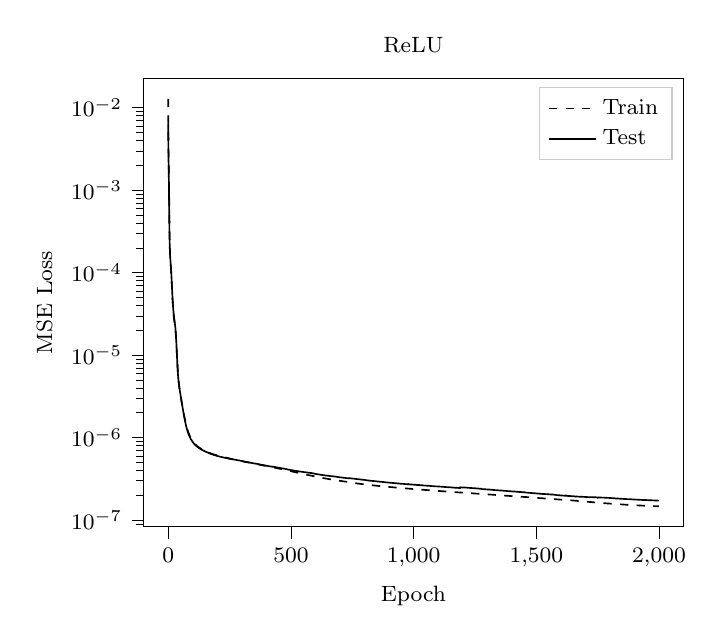
\begin{tikzpicture}

\begin{axis}[
legend cell align={left},
legend style={fill opacity=0.8, draw opacity=1, text opacity=1, draw=white!80!black},
log basis y={10},
tick align=outside,
tick pos=left,
title={ReLU},
x grid style={white!69.0196078431373!black},
xlabel={Epoch},
xmin=-99.95, xmax=2098.95,
xtick style={color=black},
y grid style={white!69.0196078431373!black},
ylabel={MSE Loss},
ymin=8.3060556203195e-08, ymax=0.0226737604172119,
ymode=log,
ytick style={color=black}
]
\addplot [semithick, black, dashed]
table {%
0 0.0128359138444066
1 0.00406811961205676
2 0.00221776218200102
3 0.00152627947740257
4 0.000869210763950832
5 0.000429490351874847
6 0.000256430144363549
7 0.000193489259458147
8 0.000159836590173654
9 0.000142019945189531
10 0.000129007256793557
11 0.000117138518267893
12 0.000105471455033694
13 9.37827313246089e-05
14 8.22589103336213e-05
15 7.13029772959999e-05
16 6.1415624084475e-05
17 5.3027559290058e-05
18 4.6298477172968e-05
19 4.10176366149244e-05
20 3.64308621828968e-05
21 3.31020509165683e-05
22 3.06825488805771e-05
23 2.8784052267838e-05
24 2.71935984428637e-05
25 2.57768373439831e-05
26 2.44650239310431e-05
27 2.31985326854556e-05
28 2.19409173314489e-05
29 2.06712553372199e-05
30 1.93696360001923e-05
31 1.80376509060807e-05
32 1.64094494193705e-05
33 1.45603561318239e-05
34 1.27872803000173e-05
35 1.11557179093325e-05
36 9.70921840917072e-06
37 8.46602692877241e-06
38 7.42971785643931e-06
39 6.59923705165966e-06
40 5.94965648508605e-06
41 5.44178499137615e-06
42 5.04196725398742e-06
43 4.71988363142373e-06
44 4.44941153807576e-06
45 4.21297154969125e-06
46 3.97091369615055e-06
47 3.78521997726011e-06
48 3.61609793606021e-06
49 3.45850858462882e-06
50 3.31160191757363e-06
51 3.17369637906495e-06
52 3.04450260318845e-06
53 2.92049022283436e-06
54 2.80214357240993e-06
55 2.69049423906154e-06
56 2.58622111073237e-06
57 2.48662982522774e-06
58 2.39208004813918e-06
59 2.30242519660351e-06
60 2.21742543777736e-06
61 2.13687340925617e-06
62 2.05999348276009e-06
63 1.98663157766532e-06
64 1.91840384792386e-06
65 1.85147106714112e-06
66 1.78930534508481e-06
67 1.73013427024671e-06
68 1.67454512279619e-06
69 1.62270763445349e-06
70 1.57398869492908e-06
71 1.52842072111525e-06
72 1.4852267215133e-06
73 1.44413795050014e-06
74 1.40627984944786e-06
75 1.36986447498089e-06
76 1.33475525311155e-06
77 1.30223323319001e-06
78 1.27158411430628e-06
79 1.24230728559382e-06
80 1.21496348251071e-06
81 1.1894506600072e-06
82 1.16576555632264e-06
83 1.14292291345919e-06
84 1.12203104029618e-06
85 1.10188948323753e-06
86 1.08292770786989e-06
87 1.06497326891031e-06
88 1.04840461335698e-06
89 1.03269330051603e-06
90 1.01698759053193e-06
91 1.00309512390595e-06
92 9.88916981896182e-07
93 9.75377727769455e-07
94 9.6289804420735e-07
95 9.5178445133115e-07
96 9.40547043398965e-07
97 9.29320102869724e-07
98 9.19224969607058e-07
99 9.09362678839898e-07
100 9.00760616332263e-07
101 8.91677312523598e-07
102 8.83358202798945e-07
103 8.7541410894687e-07
104 8.67818650164054e-07
105 8.60540775903473e-07
106 8.53664071399862e-07
107 8.47105686005989e-07
108 8.40799016799565e-07
109 8.34772250925653e-07
110 8.28988821496068e-07
111 8.23431996309409e-07
112 8.18056938896916e-07
113 8.12813703561233e-07
114 8.07828728369486e-07
115 8.03024243964501e-07
116 7.98377929925209e-07
117 7.93822158300372e-07
118 7.89469017917099e-07
119 7.8525374803462e-07
120 7.81149035503859e-07
121 7.77039519164191e-07
122 7.73208100383727e-07
123 7.69387711102354e-07
124 7.65666616501903e-07
125 7.61996876690318e-07
126 7.58383085326386e-07
127 7.54953229204602e-07
128 7.5161359521303e-07
129 7.48366523026789e-07
130 7.45194466219345e-07
131 7.41907941517184e-07
132 7.38387156445697e-07
133 7.35193854751515e-07
134 7.3226554457051e-07
135 7.29248398840809e-07
136 7.26341062176061e-07
137 7.23518060908646e-07
138 7.20833158993628e-07
139 7.18008437729622e-07
140 7.15079443153854e-07
141 7.12426657145215e-07
142 7.09709738089259e-07
143 7.07091793771042e-07
144 7.04633227798013e-07
145 7.02308290925657e-07
146 6.99840673831886e-07
147 6.97486854477347e-07
148 6.95209882849213e-07
149 6.92861825939417e-07
150 6.90704266872899e-07
151 6.88582144817929e-07
152 6.86111019234659e-07
153 6.84080939095111e-07
154 6.81975838517701e-07
155 6.79974541526462e-07
156 6.77959332790579e-07
157 6.76050047047738e-07
158 6.74017413103911e-07
159 6.72160598156779e-07
160 6.7017619542753e-07
161 6.68461542090881e-07
162 6.66575790489787e-07
163 6.64879856913103e-07
164 6.62985953709949e-07
165 6.6163600506286e-07
166 6.59435483271409e-07
167 6.57632066648262e-07
168 6.55575177276546e-07
169 6.54015729338653e-07
170 6.52307282223319e-07
171 6.504013251174e-07
172 6.46996461455274e-07
173 6.45045825507395e-07
174 6.43091596728596e-07
175 6.41354103819935e-07
176 6.39775814747168e-07
177 6.38218029919813e-07
178 6.36537369857138e-07
179 6.35115712441348e-07
180 6.33563209802901e-07
181 6.32300194652657e-07
182 6.30609901833168e-07
183 6.29600763673466e-07
184 6.27879526405195e-07
185 6.26514845080806e-07
186 6.25209512548963e-07
187 6.23535240336537e-07
188 6.22593528348148e-07
189 6.20840004998513e-07
190 6.19957963593265e-07
191 6.18262787398294e-07
192 6.17415837567137e-07
193 6.15776178662486e-07
194 6.14971566434974e-07
195 6.13444837298971e-07
196 6.12671803025933e-07
197 6.11204517156239e-07
198 6.10332435044825e-07
199 6.08851165878832e-07
200 6.080204561556e-07
201 6.06559192959821e-07
202 6.05760007701406e-07
203 6.04330644478068e-07
204 6.03280801200867e-07
205 6.01772887307561e-07
206 6.01124246642826e-07
207 5.99515939484263e-07
208 5.98675602759613e-07
209 5.9747211136596e-07
210 5.96390205643615e-07
211 5.95324714780077e-07
212 5.94377064487617e-07
213 5.93298088872984e-07
214 5.92175063729883e-07
215 5.91118195501394e-07
216 5.90146642139189e-07
217 5.89021899926934e-07
218 5.87992171404039e-07
219 5.87068497154064e-07
220 5.8602671730057e-07
221 5.85054058404921e-07
222 5.84006577440732e-07
223 5.82988822685593e-07
224 5.81989438828146e-07
225 5.81001877193899e-07
226 5.80024892542497e-07
227 5.79078803255584e-07
228 5.78110301987067e-07
229 5.77146334379108e-07
230 5.76185671306462e-07
231 5.75260986451553e-07
232 5.74307557812404e-07
233 5.73343675355886e-07
234 5.72410307597693e-07
235 5.71375916948114e-07
236 5.70444772321821e-07
237 5.69523908040992e-07
238 5.68677597769351e-07
239 5.67770445883298e-07
240 5.66866436670921e-07
241 5.65970691070561e-07
242 5.65123066863293e-07
243 5.64223408431985e-07
244 5.63306641481631e-07
245 5.6239256639401e-07
246 5.61538256064864e-07
247 5.606653090382e-07
248 5.59801215572975e-07
249 5.58943027954228e-07
250 5.58119654584743e-07
251 5.57285070087232e-07
252 5.5639160026999e-07
253 5.55517061400224e-07
254 5.54651886858437e-07
255 5.53784663139822e-07
256 5.53118923008356e-07
257 5.52271083662959e-07
258 5.51392261499473e-07
259 5.50661146789366e-07
260 5.49797288456943e-07
261 5.48924100115755e-07
262 5.48088413736991e-07
263 5.47227847107479e-07
264 5.46406514317255e-07
265 5.45611903149279e-07
266 5.44801076742374e-07
267 5.43925651868449e-07
268 5.43103572738346e-07
269 5.42293245572978e-07
270 5.4148437953927e-07
271 5.40699907702447e-07
272 5.39910273388955e-07
273 5.39133814939419e-07
274 5.38363875776326e-07
275 5.37582890757449e-07
276 5.36826901495147e-07
277 5.3603802076907e-07
278 5.35316970584177e-07
279 5.34529481910795e-07
280 5.33722675925219e-07
281 5.32918683234129e-07
282 5.32152425847698e-07
283 5.31394477121694e-07
284 5.30640270071103e-07
285 5.29907005429209e-07
286 5.29116395270535e-07
287 5.28346645850775e-07
288 5.27513266220581e-07
289 5.26773149360338e-07
290 5.26038264595741e-07
291 5.25316868134951e-07
292 5.24571295159149e-07
293 5.23829740870951e-07
294 5.23106379560545e-07
295 5.22383499131251e-07
296 5.2166716473323e-07
297 5.20962232855027e-07
298 5.20257276349412e-07
299 5.19555759524337e-07
300 5.18861061692633e-07
301 5.18167190975305e-07
302 5.17407352376154e-07
303 5.16758486270419e-07
304 5.16134349624053e-07
305 5.15409096962571e-07
306 5.1471261633651e-07
307 5.13997151728063e-07
308 5.13282595179021e-07
309 5.12469787608438e-07
310 5.11740900790869e-07
311 5.10916394645733e-07
312 5.10398340495044e-07
313 5.09615481561809e-07
314 5.0890788187985e-07
315 5.08135385487662e-07
316 5.07396071839139e-07
317 5.0667694905826e-07
318 5.06027933980135e-07
319 5.05363481877907e-07
320 5.04778821508012e-07
321 5.04100044608435e-07
322 5.03420945790367e-07
323 5.02913110352665e-07
324 5.02204066606282e-07
325 5.01519381444382e-07
326 5.0075652430337e-07
327 5.00041955618258e-07
328 4.99340976446661e-07
329 4.98837331861068e-07
330 4.98114730092425e-07
331 4.97396278106521e-07
332 4.96683979335444e-07
333 4.95992166946735e-07
334 4.95327224157904e-07
335 4.94672618728487e-07
336 4.94005201645109e-07
337 4.93368763699209e-07
338 4.92711109188804e-07
339 4.92064750176269e-07
340 4.91377320216202e-07
341 4.90734373599366e-07
342 4.90094236084815e-07
343 4.8923520419919e-07
344 4.88491250393963e-07
345 4.87911429033261e-07
346 4.86993086525445e-07
347 4.86201224958904e-07
348 4.85454121516682e-07
349 4.84715875060715e-07
350 4.83999491038389e-07
351 4.8330461555679e-07
352 4.82610435923903e-07
353 4.81942027434457e-07
354 4.81273281664585e-07
355 4.80657552941466e-07
356 4.79991086152154e-07
357 4.79426202517175e-07
358 4.78786983705959e-07
359 4.78136694752607e-07
360 4.77479370928791e-07
361 4.76951999701214e-07
362 4.76438385987876e-07
363 4.75759972076162e-07
364 4.75071433612584e-07
365 4.74538327580376e-07
366 4.73795507247132e-07
367 4.73118962915464e-07
368 4.72461489309239e-07
369 4.71825251139535e-07
370 4.71192496632966e-07
371 4.70559365041368e-07
372 4.70058532613393e-07
373 4.69410172783569e-07
374 4.68776403550919e-07
375 4.67982378282272e-07
376 4.67325791433382e-07
377 4.66681011914716e-07
378 4.66014211454535e-07
379 4.65348282233435e-07
380 4.64814711989447e-07
381 4.64148458462432e-07
382 4.63576862159698e-07
383 4.62930432362896e-07
384 4.62302280809013e-07
385 4.61679847362006e-07
386 4.61104624704944e-07
387 4.60824521880454e-07
388 4.60142321898616e-07
389 4.59398271928535e-07
390 4.58787464964416e-07
391 4.58134393070964e-07
392 4.57507636880905e-07
393 4.56882881110232e-07
394 4.5631434277027e-07
395 4.55657936043963e-07
396 4.54997403451785e-07
397 4.54597877237006e-07
398 4.53956164321312e-07
399 4.53263333653808e-07
400 4.52610636330064e-07
401 4.51975337526278e-07
402 4.51166000871694e-07
403 4.50556313722927e-07
404 4.49943631167571e-07
405 4.50224415246225e-07
406 4.49388958884356e-07
407 4.48679926989826e-07
408 4.47983747477565e-07
409 4.47319951319969e-07
410 4.46692041819574e-07
411 4.46043008082597e-07
412 4.45379412937541e-07
413 4.44756290605142e-07
414 4.44137515501097e-07
415 4.43530492361788e-07
416 4.42895292664502e-07
417 4.42246661634726e-07
418 4.4161888378369e-07
419 4.41050250699959e-07
420 4.4041967524322e-07
421 4.39794044325481e-07
422 4.39187426295007e-07
423 4.38575338435498e-07
424 4.37924559278713e-07
425 4.37397801690054e-07
426 4.36789211121891e-07
427 4.36235071774149e-07
428 4.35714181989511e-07
429 4.35064805230923e-07
430 4.3441796375987e-07
431 4.33821461186312e-07
432 4.33212344105982e-07
433 4.3256776783096e-07
434 4.31979589833986e-07
435 4.31346918034592e-07
436 4.30742508925164e-07
437 4.30014452831529e-07
438 4.29212309612126e-07
439 4.28535380322614e-07
440 4.2784484142544e-07
441 4.27162711716278e-07
442 4.2654244050766e-07
443 4.25920634356203e-07
444 4.25289486614133e-07
445 4.24664052573576e-07
446 4.24054528849638e-07
447 4.23444578245835e-07
448 4.22825500720592e-07
449 4.22235647633329e-07
450 4.21641495776726e-07
451 4.21042936622484e-07
452 4.204042555358e-07
453 4.19785291612129e-07
454 4.19165474724537e-07
455 4.18587373061996e-07
456 4.17983689530388e-07
457 4.17366091724602e-07
458 4.16813378095071e-07
459 4.16216044001771e-07
460 4.1563661304167e-07
461 4.15065193166697e-07
462 4.14440477527478e-07
463 4.137947071996e-07
464 4.13075351730186e-07
465 4.12454505095639e-07
466 4.11876993922533e-07
467 4.1130139980794e-07
468 4.10712745221531e-07
469 4.10157508312636e-07
470 4.09618700686565e-07
471 4.0901640734603e-07
472 4.08388660346759e-07
473 4.07808872111559e-07
474 4.07190228571608e-07
475 4.06595403376286e-07
476 4.06010637888698e-07
477 4.05392317176734e-07
478 4.04781765979578e-07
479 4.04163714279093e-07
480 4.03598776060221e-07
481 4.03019477431599e-07
482 4.0240480798559e-07
483 4.0181467062439e-07
484 4.01190572162591e-07
485 4.00669628959349e-07
486 4.00093216029518e-07
487 3.99534549217151e-07
488 3.98832486453671e-07
489 3.98232996289494e-07
490 3.97586432200114e-07
491 3.96999277043619e-07
492 3.96335612961707e-07
493 3.95738804854773e-07
494 3.95199794851919e-07
495 3.94601066957989e-07
496 3.93942960840832e-07
497 3.9341726065345e-07
498 3.92822267642146e-07
499 3.92249883688578e-07
500 3.9166239578492e-07
501 3.90943145731626e-07
502 3.90417924037934e-07
503 3.89788243779776e-07
504 3.89221085768554e-07
505 3.88712462026319e-07
506 3.88139190917514e-07
507 3.87384185444262e-07
508 3.8658280821835e-07
509 3.85974133635614e-07
510 3.85345149737759e-07
511 3.84755621880117e-07
512 3.84093485990888e-07
513 3.83513560478832e-07
514 3.82928092875545e-07
515 3.82343274367258e-07
516 3.81772343004627e-07
517 3.81215974144311e-07
518 3.80635759938741e-07
519 3.80127739830982e-07
520 3.79530231583658e-07
521 3.78973119623538e-07
522 3.78421440586862e-07
523 3.77808645694699e-07
524 3.77222886726258e-07
525 3.76684518130332e-07
526 3.76060851081661e-07
527 3.75412971578726e-07
528 3.74828130603078e-07
529 3.74236345834333e-07
530 3.73695037055199e-07
531 3.73073411736868e-07
532 3.72465256930354e-07
533 3.71768114604265e-07
534 3.71223410738253e-07
535 3.70558538918431e-07
536 3.69985989095767e-07
537 3.69416098607189e-07
538 3.68824209559193e-07
539 3.68246500883629e-07
540 3.67674652096639e-07
541 3.67146909241001e-07
542 3.6655390564988e-07
543 3.65992903496704e-07
544 3.65448769613863e-07
545 3.64904883639383e-07
546 3.64338433428202e-07
547 3.63806817304635e-07
548 3.63257377458126e-07
549 3.62574539664706e-07
550 3.62068634359503e-07
551 3.61473358509556e-07
552 3.60935242895266e-07
553 3.60413636357748e-07
554 3.59868972850563e-07
555 3.5935385152186e-07
556 3.58844249333856e-07
557 3.58326943697307e-07
558 3.57797470698529e-07
559 3.57330856189719e-07
560 3.56872281628284e-07
561 3.56368487672398e-07
562 3.55836359986483e-07
563 3.55332234633465e-07
564 3.54824446645807e-07
565 3.54339146753091e-07
566 3.53827280022756e-07
567 3.53325290390671e-07
568 3.52850746850208e-07
569 3.52336466477254e-07
570 3.51856831954933e-07
571 3.5136100875377e-07
572 3.50893734022861e-07
573 3.50407004418685e-07
574 3.4989447030398e-07
575 3.49443885625078e-07
576 3.4893881971243e-07
577 3.48500343307023e-07
578 3.4798630669286e-07
579 3.47510213757118e-07
580 3.47052929782876e-07
581 3.46572929046829e-07
582 3.46100820763695e-07
583 3.45635644279696e-07
584 3.45174572856877e-07
585 3.44720079127114e-07
586 3.44251229549286e-07
587 3.43796819834097e-07
588 3.43215964477395e-07
589 3.42688052199946e-07
590 3.42216255234007e-07
591 3.41808416024492e-07
592 3.41212007285208e-07
593 3.40706088309162e-07
594 3.40231385706602e-07
595 3.3973816373134e-07
596 3.39256642760688e-07
597 3.38761948015076e-07
598 3.38252847200238e-07
599 3.37764319738199e-07
600 3.37289797997187e-07
601 3.36832910235785e-07
602 3.36301321624433e-07
603 3.35731551629692e-07
604 3.35256483978696e-07
605 3.34784972508828e-07
606 3.34324919933238e-07
607 3.33847983526425e-07
608 3.33368957925018e-07
609 3.32913002822011e-07
610 3.32462384264431e-07
611 3.31984051385348e-07
612 3.31562530178076e-07
613 3.31118336518443e-07
614 3.30674347267745e-07
615 3.30218415513173e-07
616 3.29806052974391e-07
617 3.29311662270015e-07
618 3.28869587505665e-07
619 3.28467940903465e-07
620 3.27985743709291e-07
621 3.27568215709562e-07
622 3.27144061799345e-07
623 3.26670766185089e-07
624 3.26214176098461e-07
625 3.25802174742762e-07
626 3.25410245523017e-07
627 3.24975043511699e-07
628 3.24551212329993e-07
629 3.24158174407785e-07
630 3.23716544528452e-07
631 3.23299862060367e-07
632 3.22898985729125e-07
633 3.22488403895704e-07
634 3.22097345872407e-07
635 3.21700158878002e-07
636 3.21304454558913e-07
637 3.20912313469535e-07
638 3.20524564074276e-07
639 3.20136042191166e-07
640 3.19752844077925e-07
641 3.19376165165863e-07
642 3.18992066596024e-07
643 3.18628257616638e-07
644 3.18242471507801e-07
645 3.17883358164295e-07
646 3.17517607541617e-07
647 3.17189173131283e-07
648 3.16752779781382e-07
649 3.16441293151115e-07
650 3.15991993588227e-07
651 3.15567727056987e-07
652 3.15198235242065e-07
653 3.14852366315677e-07
654 3.14477423572157e-07
655 3.14116288961941e-07
656 3.13751376125992e-07
657 3.13407868560489e-07
658 3.13042362492411e-07
659 3.1268381887628e-07
660 3.12334496982203e-07
661 3.11969507151844e-07
662 3.1163067758655e-07
663 3.11306783956411e-07
664 3.10919280082089e-07
665 3.10583744706605e-07
666 3.10250059655459e-07
667 3.09937706305163e-07
668 3.09573450948619e-07
669 3.09204214246961e-07
670 3.08850459617815e-07
671 3.08537095591532e-07
672 3.08225946909602e-07
673 3.07908969560344e-07
674 3.07560297102327e-07
675 3.0723168808322e-07
676 3.06905842663241e-07
677 3.06626207304816e-07
678 3.06256743982658e-07
679 3.05940740773281e-07
680 3.05711705024692e-07
681 3.05346728438849e-07
682 3.05022357409257e-07
683 3.04787608797596e-07
684 3.04591078773342e-07
685 3.04243192218223e-07
686 3.03902760222741e-07
687 3.03562333655805e-07
688 3.03246627694875e-07
689 3.02922987273746e-07
690 3.02614198247397e-07
691 3.02081464738535e-07
692 3.01742485603995e-07
693 3.01437276149841e-07
694 3.01078963033774e-07
695 3.00749295163882e-07
696 3.00478578765251e-07
697 3.00096437030106e-07
698 2.99800604125267e-07
699 2.99512212393438e-07
700 2.99188646494031e-07
701 2.98825807448111e-07
702 2.98531001078572e-07
703 2.98287063074554e-07
704 2.98012047025509e-07
705 2.97674375701717e-07
706 2.97391246348866e-07
707 2.97087627117776e-07
708 2.96822007285868e-07
709 2.96534653557501e-07
710 2.96241515030715e-07
711 2.95766508685347e-07
712 2.95477427869173e-07
713 2.95199973777471e-07
714 2.94934526451129e-07
715 2.94622614532614e-07
716 2.94349123265647e-07
717 2.94059612983233e-07
718 2.93763836197059e-07
719 2.93480562305604e-07
720 2.93202444495932e-07
721 2.92916106459984e-07
722 2.92623508840961e-07
723 2.92435868473717e-07
724 2.92131600772905e-07
725 2.91845484383657e-07
726 2.91578852696261e-07
727 2.91303842161028e-07
728 2.91009091881733e-07
729 2.90722125015463e-07
730 2.90455377040644e-07
731 2.90185338116089e-07
732 2.8992908158898e-07
733 2.89663138232754e-07
734 2.8940803167643e-07
735 2.89136017798342e-07
736 2.889206294725e-07
737 2.88737842566888e-07
738 2.88997667908575e-07
739 2.88562024607586e-07
740 2.88228037263139e-07
741 2.87892525449251e-07
742 2.87586055392808e-07
743 2.8728029188585e-07
744 2.86980700195727e-07
745 2.86744340243672e-07
746 2.8622192211003e-07
747 2.85925212054394e-07
748 2.85634268323065e-07
749 2.85337112515549e-07
750 2.8511037254475e-07
751 2.84853912376093e-07
752 2.84023656476506e-07
753 2.83497718470471e-07
754 2.83116851676368e-07
755 2.82695359175023e-07
756 2.82512347510533e-07
757 2.82085629521589e-07
758 2.81725797435683e-07
759 2.81449778896103e-07
760 2.8105877230189e-07
761 2.80944373514558e-07
762 2.80682355423778e-07
763 2.80297662115458e-07
764 2.79940790193223e-07
765 2.79655734573225e-07
766 2.7931117253388e-07
767 2.78977283855397e-07
768 2.78635521198112e-07
769 2.78352544214044e-07
770 2.7819338988877e-07
771 2.77889544165078e-07
772 2.77548593075494e-07
773 2.77264688477885e-07
774 2.7704935030215e-07
775 2.76729705390721e-07
776 2.7645308894364e-07
777 2.76195476729413e-07
778 2.7594944073428e-07
779 2.75716891124489e-07
780 2.75467336976476e-07
781 2.75225335968798e-07
782 2.75062229206924e-07
783 2.7480055271667e-07
784 2.74580447268136e-07
785 2.74362289260921e-07
786 2.74111401481036e-07
787 2.73876008265006e-07
788 2.73605013845213e-07
789 2.73413644165998e-07
790 2.73188405444103e-07
791 2.72918508599673e-07
792 2.72716296422004e-07
793 2.72480284039034e-07
794 2.72285307730158e-07
795 2.72149884011696e-07
796 2.71952939314701e-07
797 2.71704815986595e-07
798 2.71441972643061e-07
799 2.71195177930395e-07
800 2.7097320317182e-07
801 2.70770428784317e-07
802 2.70505914016894e-07
803 2.70232581939922e-07
804 2.69978283682804e-07
805 2.69613692850612e-07
806 2.6923754116126e-07
807 2.68977236729029e-07
808 2.68752260268457e-07
809 2.68544625768641e-07
810 2.68373911282538e-07
811 2.68163501999652e-07
812 2.67927181553773e-07
813 2.67719987007808e-07
814 2.67517097881864e-07
815 2.67310931533871e-07
816 2.67105253826116e-07
817 2.66903428638443e-07
818 2.66692599950602e-07
819 2.66481964402487e-07
820 2.66284019161844e-07
821 2.66081862648093e-07
822 2.66027550424042e-07
823 2.65821824157797e-07
824 2.65619061863731e-07
825 2.65410844818348e-07
826 2.65213099211792e-07
827 2.65021856961312e-07
828 2.64826372728066e-07
829 2.64633269267733e-07
830 2.64446708726496e-07
831 2.64248240071652e-07
832 2.64059634162095e-07
833 2.63878327388056e-07
834 2.63682958788536e-07
835 2.63493734607323e-07
836 2.63316504145905e-07
837 2.63118264641093e-07
838 2.62901429465501e-07
839 2.62730751714457e-07
840 2.62452709399952e-07
841 2.62270763101924e-07
842 2.62094237520216e-07
843 2.61916025223741e-07
844 2.61752447649144e-07
845 2.61570247680254e-07
846 2.61391405729228e-07
847 2.61197685773595e-07
848 2.61104773478849e-07
849 2.60918261439258e-07
850 2.60724515214861e-07
851 2.60535269994477e-07
852 2.60345671463824e-07
853 2.60163190716867e-07
854 2.59979377318587e-07
855 2.59807215748253e-07
856 2.59638242802396e-07
857 2.59457045409306e-07
858 2.5929549951087e-07
859 2.59103974563857e-07
860 2.58932327128036e-07
861 2.58767719678588e-07
862 2.58579918060775e-07
863 2.58410764914174e-07
864 2.58235526878536e-07
865 2.58068606832751e-07
866 2.579093218813e-07
867 2.5772559851589e-07
868 2.5755975129016e-07
869 2.57416757627027e-07
870 2.57236482134715e-07
871 2.57065044301896e-07
872 2.56887864409805e-07
873 2.56699708664598e-07
874 2.56526549620162e-07
875 2.56373737975935e-07
876 2.56201032037495e-07
877 2.56034790240278e-07
878 2.55873794714034e-07
879 2.55705920480409e-07
880 2.55417128485647e-07
881 2.55229956422909e-07
882 2.55085984754544e-07
883 2.54928232898521e-07
884 2.54779993753118e-07
885 2.54592056549541e-07
886 2.54439689939545e-07
887 2.5426591516009e-07
888 2.54102271377121e-07
889 2.53930725016005e-07
890 2.53764556227054e-07
891 2.53614336365615e-07
892 2.53452076336202e-07
893 2.532692485957e-07
894 2.53125733742365e-07
895 2.52976690667595e-07
896 2.528093443388e-07
897 2.52656056844103e-07
898 2.52499306505172e-07
899 2.52364507723257e-07
900 2.52203973225562e-07
901 2.52031071774184e-07
902 2.518835791534e-07
903 2.51714416926063e-07
904 2.51555577612805e-07
905 2.51338153084646e-07
906 2.51199765898491e-07
907 2.51049156986483e-07
908 2.50885086643393e-07
909 2.50740681572381e-07
910 2.50585756418786e-07
911 2.50420220616832e-07
912 2.50275292266622e-07
913 2.50121281410998e-07
914 2.4995576485054e-07
915 2.49676279501898e-07
916 2.49520305203532e-07
917 2.49378198027728e-07
918 2.4922392374549e-07
919 2.49076048127961e-07
920 2.48927619701078e-07
921 2.48776921417004e-07
922 2.48630119202176e-07
923 2.48482846032516e-07
924 2.48332861993106e-07
925 2.48184320888356e-07
926 2.48036973083288e-07
927 2.47890264816419e-07
928 2.4774389887483e-07
929 2.47597746444228e-07
930 2.47460814819078e-07
931 2.47319833690085e-07
932 2.47171875763286e-07
933 2.46986154522233e-07
934 2.46846625991282e-07
935 2.46710934568739e-07
936 2.46565559500311e-07
937 2.46414631448033e-07
938 2.46274233148824e-07
939 2.46133543761573e-07
940 2.45993646721843e-07
941 2.45851855076751e-07
942 2.4571178909838e-07
943 2.45570187580313e-07
944 2.45427655464425e-07
945 2.4528916037525e-07
946 2.45144313090862e-07
947 2.45008457774531e-07
948 2.44778515678945e-07
949 2.44709522988273e-07
950 2.44557021623848e-07
951 2.44444680092215e-07
952 2.44300696401467e-07
953 2.44156826106234e-07
954 2.44018879300256e-07
955 2.43875476478195e-07
956 2.43733082527342e-07
957 2.43594031232419e-07
958 2.43454059834391e-07
959 2.43317650365782e-07
960 2.43178574322656e-07
961 2.43043392202935e-07
962 2.42901336989121e-07
963 2.42752515198674e-07
964 2.42617944856249e-07
965 2.42478849045824e-07
966 2.42350840103711e-07
967 2.42212682998399e-07
968 2.42075261638774e-07
969 2.41937336305398e-07
970 2.41740744577612e-07
971 2.41667918423616e-07
972 2.41518041917743e-07
973 2.41401504226246e-07
974 2.41222875168035e-07
975 2.41124690397498e-07
976 2.40940309865323e-07
977 2.40789396293906e-07
978 2.40686851775251e-07
979 2.4058535476712e-07
980 2.40380043535993e-07
981 2.40305805455421e-07
982 2.40108319552235e-07
983 2.40031877538627e-07
984 2.39894949039865e-07
985 2.3973578581149e-07
986 2.39611460926881e-07
987 2.39439004758424e-07
988 2.3930055066046e-07
989 2.39153940320591e-07
990 2.38980053701709e-07
991 2.38914729784767e-07
992 2.38757834530645e-07
993 2.38612148095285e-07
994 2.3841948619463e-07
995 2.38344357995857e-07
996 2.38203236882839e-07
997 2.38060229719395e-07
998 2.37923468709766e-07
999 2.37793798923747e-07
1000 2.37646189845009e-07
1001 2.37599634857588e-07
1002 2.37371781985019e-07
1003 2.37256684719966e-07
1004 2.3710381680786e-07
1005 2.37030779430825e-07
1006 2.36854548504084e-07
1007 2.36789443157193e-07
1008 2.36603149716075e-07
1009 2.36586189146237e-07
1010 2.36392693182097e-07
1011 2.36260623339035e-07
1012 2.36101812092215e-07
1013 2.36086071886632e-07
1014 2.35904035029932e-07
1015 2.35725191885194e-07
1016 2.35685808050334e-07
1017 2.35596702900409e-07
1018 2.35438702382851e-07
1019 2.35246950623491e-07
1020 2.35075611456637e-07
1021 2.35099903790115e-07
1022 2.3487148752821e-07
1023 2.34750061487432e-07
1024 2.34573643794533e-07
1025 2.34564620235744e-07
1026 2.34471072538156e-07
1027 2.34354624211619e-07
1028 2.34128390850685e-07
1029 2.33955763171423e-07
1030 2.33922607776549e-07
1031 2.33783959046718e-07
1032 2.33714321531409e-07
1033 2.33685208733903e-07
1034 2.33539281111916e-07
1035 2.33392913706609e-07
1036 2.33203155495687e-07
1037 2.331949610479e-07
1038 2.32991934915106e-07
1039 2.32850305849297e-07
1040 2.32765783117372e-07
1041 2.32670341915764e-07
1042 2.32657039475725e-07
1043 2.32462914603104e-07
1044 2.32303914394549e-07
1045 2.32177753510143e-07
1046 2.32038218555886e-07
1047 2.31941964251803e-07
1048 2.31735411837519e-07
1049 2.3166942881403e-07
1050 2.31621027936058e-07
1051 2.31475059614183e-07
1052 2.31326241298291e-07
1053 2.31239147751694e-07
1054 2.31119690745629e-07
1055 2.31017140592371e-07
1056 2.3086940776551e-07
1057 2.30697620096976e-07
1058 2.30660508172775e-07
1059 2.30563432516817e-07
1060 2.30397781528779e-07
1061 2.30417078178391e-07
1062 2.30317154283455e-07
1063 2.30162277986778e-07
1064 2.30063518721124e-07
1065 2.29899269129419e-07
1066 2.29807306638463e-07
1067 2.29664271131469e-07
1068 2.29567998907498e-07
1069 2.29445193149047e-07
1070 2.29313082712679e-07
1071 2.29218835350764e-07
1072 2.2906969297054e-07
1073 2.28964648627539e-07
1074 2.28864435037224e-07
1075 2.28717713547155e-07
1076 2.2863567138387e-07
1077 2.28499026974305e-07
1078 2.28409063225854e-07
1079 2.28298539020955e-07
1080 2.28191649313203e-07
1081 2.28083222189923e-07
1082 2.27955539990887e-07
1083 2.27841008324958e-07
1084 2.2773020606337e-07
1085 2.27610032744963e-07
1086 2.27501331949043e-07
1087 2.27376409974056e-07
1088 2.2726379945226e-07
1089 2.27137682820455e-07
1090 2.26827840933197e-07
1091 2.26754384584638e-07
1092 2.26650240975346e-07
1093 2.26534615457297e-07
1094 2.26412695525369e-07
1095 2.26291264908696e-07
1096 2.26169796015085e-07
1097 2.26040921411652e-07
1098 2.25922023474823e-07
1099 2.25797209253642e-07
1100 2.25675585596719e-07
1101 2.25561426347554e-07
1102 2.254305840097e-07
1103 2.25311821019147e-07
1104 2.25195945944279e-07
1105 2.25079520305371e-07
1106 2.24965323099013e-07
1107 2.24867464545753e-07
1108 2.24762359117392e-07
1109 2.24626370084025e-07
1110 2.24508406084567e-07
1111 2.24395075314021e-07
1112 2.24277390778127e-07
1113 2.24158637927019e-07
1114 2.2404539223686e-07
1115 2.23920358827456e-07
1116 2.23808280111371e-07
1117 2.23686827183656e-07
1118 2.2356966128001e-07
1119 2.23456709292691e-07
1120 2.23334162825495e-07
1121 2.23228413595677e-07
1122 2.23115099544202e-07
1123 2.23002317440546e-07
1124 2.22879026416933e-07
1125 2.22769490122232e-07
1126 2.22664080226309e-07
1127 2.2253616578638e-07
1128 2.22430343903568e-07
1129 2.223116337845e-07
1130 2.22204481723054e-07
1131 2.22094232434245e-07
1132 2.21976963509007e-07
1133 2.21866377820845e-07
1134 2.21753350238885e-07
1135 2.21644285254285e-07
1136 2.21531433545863e-07
1137 2.21416343521241e-07
1138 2.21307805006177e-07
1139 2.21198763370012e-07
1140 2.21085268165666e-07
1141 2.20975650925936e-07
1142 2.20881519460647e-07
1143 2.20775239149873e-07
1144 2.20637945012925e-07
1145 2.20559710285784e-07
1146 2.20444337422521e-07
1147 2.20324321794863e-07
1148 2.20211126375602e-07
1149 2.201148186316e-07
1150 2.19997589574916e-07
1151 2.1989982777626e-07
1152 2.19791165335437e-07
1153 2.196815010862e-07
1154 2.19573701976117e-07
1155 2.19463932438657e-07
1156 2.19359349159731e-07
1157 2.19249752198891e-07
1158 2.19142922851745e-07
1159 2.19035697959669e-07
1160 2.18929460672257e-07
1161 2.18930828516761e-07
1162 2.18828259697545e-07
1163 2.18708604258211e-07
1164 2.18593607570483e-07
1165 2.18480611941629e-07
1166 2.1837456065299e-07
1167 2.18264942468238e-07
1168 2.18158639007981e-07
1169 2.18042133006691e-07
1170 2.17949583657173e-07
1171 2.17841640782979e-07
1172 2.17736934885693e-07
1173 2.17629174635192e-07
1174 2.17524212679621e-07
1175 2.1741689277377e-07
1176 2.1731769705724e-07
1177 2.17213480382839e-07
1178 2.1710752405113e-07
1179 2.17002218498408e-07
1180 2.16897231283042e-07
1181 2.16794168977685e-07
1182 2.16689441295159e-07
1183 2.16586816598863e-07
1184 2.16482968788512e-07
1185 2.1638173421934e-07
1186 2.16274073231659e-07
1187 2.16172590953079e-07
1188 2.16080631012971e-07
1189 2.1599227943625e-07
1190 2.15979764696783e-07
1191 2.16017678475566e-07
1192 2.15873939545475e-07
1193 2.15748003292049e-07
1194 2.15623455886771e-07
1195 2.15515344123673e-07
1196 2.15400620767525e-07
1197 2.15292371208875e-07
1198 2.15177959709933e-07
1199 2.15071723104643e-07
1200 2.14928613999632e-07
1201 2.14839535118472e-07
1202 2.14735765474927e-07
1203 2.14574807344547e-07
1204 2.14502365381009e-07
1205 2.14412341868808e-07
1206 2.14283540159954e-07
1207 2.14210046642904e-07
1208 2.14107812681164e-07
1209 2.14021252809005e-07
1210 2.13936210762711e-07
1211 2.13915925698416e-07
1212 2.13799923876934e-07
1213 2.13669566456076e-07
1214 2.13561179556621e-07
1215 2.13467269645662e-07
1216 2.13349683882313e-07
1217 2.13256108388293e-07
1218 2.13155513392849e-07
1219 2.13042389802354e-07
1220 2.12919297460701e-07
1221 2.12815673890532e-07
1222 2.12711443602132e-07
1223 2.12652658127865e-07
1224 2.12501022431866e-07
1225 2.12420601719998e-07
1226 2.12309944174649e-07
1227 2.12366951096499e-07
1228 2.12222830079156e-07
1229 2.12110472261884e-07
1230 2.11929635618446e-07
1231 2.11879924854941e-07
1232 2.11703791869411e-07
1233 2.11653654140775e-07
1234 2.1151320120083e-07
1235 2.11419449257733e-07
1236 2.11250796276374e-07
1237 2.11202558560331e-07
1238 2.11102061150825e-07
1239 2.10944673966651e-07
1240 2.10911240309031e-07
1241 2.1076127746511e-07
1242 2.10704322974209e-07
1243 2.10567815479123e-07
1244 2.10497195574533e-07
1245 2.1040943553885e-07
1246 2.10297608973065e-07
1247 2.10163938255903e-07
1248 2.10107044765095e-07
1249 2.10013232752715e-07
1250 2.09916546062061e-07
1251 2.09774376543237e-07
1252 2.09698891929122e-07
1253 2.09622506929463e-07
1254 2.09513595876842e-07
1255 2.09421121070363e-07
1256 2.09320254114687e-07
1257 2.09215731480583e-07
1258 2.09130282691206e-07
1259 2.09036870700174e-07
1260 2.08928067813474e-07
1261 2.08838153490376e-07
1262 2.08749056248791e-07
1263 2.08652356469941e-07
1264 2.08550158639298e-07
1265 2.08489736223783e-07
1266 2.0837612094482e-07
1267 2.08276492024595e-07
1268 2.08193774028587e-07
1269 2.08094111279422e-07
1270 2.07980286397458e-07
1271 2.07888382796284e-07
1272 2.07787530371206e-07
1273 2.07656961599412e-07
1274 2.07569616925696e-07
1275 2.0746449245479e-07
1276 2.07364236295859e-07
1277 2.07165836712875e-07
1278 2.07041992617007e-07
1279 2.06997534185405e-07
1280 2.06897416155982e-07
1281 2.06792438376624e-07
1282 2.06619498243299e-07
1283 2.06613423934243e-07
1284 2.06489881819039e-07
1285 2.0638760765479e-07
1286 2.06301932017539e-07
1287 2.06185098910794e-07
1288 2.06122904430117e-07
1289 2.0603094798588e-07
1290 2.05890058659008e-07
1291 2.058426851832e-07
1292 2.05701655730195e-07
1293 2.05651675621255e-07
1294 2.05522865172725e-07
1295 2.05462758223973e-07
1296 2.05339187992593e-07
1297 2.05216017839405e-07
1298 2.05128365635687e-07
1299 2.05095285075174e-07
1300 2.04930593312724e-07
1301 2.04907038209967e-07
1302 2.04736265757788e-07
1303 2.0472843108621e-07
1304 2.04564254225659e-07
1305 2.04535793123739e-07
1306 2.04411864075382e-07
1307 2.04340191245933e-07
1308 2.04220152618007e-07
1309 2.04110330066953e-07
1310 2.04035512098244e-07
1311 2.03963682523067e-07
1312 2.03857806447161e-07
1313 2.03766906793135e-07
1314 2.03600763406087e-07
1315 2.03567661820614e-07
1316 2.03439885275714e-07
1317 2.0336518320363e-07
1318 2.032757020487e-07
1319 2.03217184783e-07
1320 2.03097577866629e-07
1321 2.03010853205399e-07
1322 2.02895738659947e-07
1323 2.02795099845332e-07
1324 2.02704501582218e-07
1325 2.02589735827985e-07
1326 2.02511892204882e-07
1327 2.02408412725674e-07
1328 2.02272598507136e-07
1329 2.0214227660631e-07
1330 2.02043033908694e-07
1331 2.01940268901524e-07
1332 2.01830009295634e-07
1333 2.01788452855567e-07
1334 2.01665288990682e-07
1335 2.01558977146021e-07
1336 2.01502488479832e-07
1337 2.01370287101099e-07
1338 2.01262453124684e-07
1339 2.01164852363434e-07
1340 2.01063925814537e-07
1341 2.00968840445626e-07
1342 2.00907314329868e-07
1343 2.00762776536578e-07
1344 2.00683564941073e-07
1345 2.00600544012275e-07
1346 2.00489199613685e-07
1347 2.00247139510168e-07
1348 2.0018000638089e-07
1349 2.00085132711081e-07
1350 1.99985089430754e-07
1351 1.99909750492111e-07
1352 1.99793285268868e-07
1353 1.99699068950565e-07
1354 1.99619168668619e-07
1355 1.99508070835464e-07
1356 1.99424367018253e-07
1357 1.99339445082103e-07
1358 1.99232693923079e-07
1359 1.99150643993562e-07
1360 1.99041314644433e-07
1361 1.9894423559208e-07
1362 1.98858898443177e-07
1363 1.98747527939247e-07
1364 1.98649745641433e-07
1365 1.98597096414233e-07
1366 1.98485464387943e-07
1367 1.9839009510747e-07
1368 1.98303617892748e-07
1369 1.98163553932318e-07
1370 1.98024752101844e-07
1371 1.9802462633578e-07
1372 1.97904007080751e-07
1373 1.97792426241961e-07
1374 1.97700932204725e-07
1375 1.97582478129732e-07
1376 1.97496014543219e-07
1377 1.97442480079246e-07
1378 1.97292501994184e-07
1379 1.97215899994774e-07
1380 1.97129082785352e-07
1381 1.97047096150982e-07
1382 1.96931914999254e-07
1383 1.96866535979723e-07
1384 1.96748979227834e-07
1385 1.96670395652632e-07
1386 1.96537504265848e-07
1387 1.96472592328689e-07
1388 1.96395970554875e-07
1389 1.96314325215496e-07
1390 1.96160989446525e-07
1391 1.96098936960709e-07
1392 1.95963414675759e-07
1393 1.95923781213025e-07
1394 1.9576923853748e-07
1395 1.95750483491963e-07
1396 1.95624758973167e-07
1397 1.95513828309402e-07
1398 1.95484114023259e-07
1399 1.95305951599778e-07
1400 1.95257116345715e-07
1401 1.95148459923189e-07
1402 1.95140374209757e-07
1403 1.95018690270388e-07
1404 1.94886642852055e-07
1405 1.94786378692413e-07
1406 1.94772436103108e-07
1407 1.94666272740562e-07
1408 1.94536682762703e-07
1409 1.94470198458419e-07
1410 1.94301135245212e-07
1411 1.94241530216743e-07
1412 1.94114599068484e-07
1413 1.94071764546777e-07
1414 1.93994561087152e-07
1415 1.93910387515928e-07
1416 1.93826246174922e-07
1417 1.93731067383851e-07
1418 1.93607339234347e-07
1419 1.93542343367881e-07
1420 1.9343740844846e-07
1421 1.93307958880951e-07
1422 1.93212855663205e-07
1423 1.9319500296433e-07
1424 1.93057864024127e-07
1425 1.93003795104119e-07
1426 1.92875757235811e-07
1427 1.92799762956497e-07
1428 1.92709066794805e-07
1429 1.92629986820236e-07
1430 1.92562667393759e-07
1431 1.92412457487023e-07
1432 1.923164970421e-07
1433 1.92212994384988e-07
1434 1.92117591787166e-07
1435 1.92054836240629e-07
1436 1.92077585573713e-07
1437 1.91970624435101e-07
1438 1.91855633147497e-07
1439 1.91738552040022e-07
1440 1.91556437243889e-07
1441 1.91566779371044e-07
1442 1.91436991002547e-07
1443 1.91359781638312e-07
1444 1.91402773523919e-07
1445 1.91267241291371e-07
1446 1.9109486520108e-07
1447 1.91051301001721e-07
1448 1.90914974176337e-07
1449 1.90833660269618e-07
1450 1.90732240533009e-07
1451 1.90663927462253e-07
1452 1.90549957004293e-07
1453 1.90516927240481e-07
1454 1.90568535209934e-07
1455 1.90464090856324e-07
1456 1.90173839605734e-07
1457 1.90063078804314e-07
1458 1.90166451851326e-07
1459 1.90337836649235e-07
1460 1.90102733085951e-07
1461 1.8997548833255e-07
1462 1.89736554936815e-07
1463 1.89701801993181e-07
1464 1.8942595669813e-07
1465 1.89337171434545e-07
1466 1.89209052699368e-07
1467 1.89201453991927e-07
1468 1.89235038845936e-07
1469 1.89176961463033e-07
1470 1.89062633360493e-07
1471 1.88726122743788e-07
1472 1.88520785847857e-07
1473 1.88483920233296e-07
1474 1.88584162799543e-07
1475 1.88440573332116e-07
1476 1.88324926952532e-07
1477 1.88138743801858e-07
1478 1.88068955395693e-07
1479 1.87984317840062e-07
1480 1.87901757342956e-07
1481 1.87818820784003e-07
1482 1.87700506828037e-07
1483 1.87608113890292e-07
1484 1.87492924730748e-07
1485 1.87428510905363e-07
1486 1.87290235636794e-07
1487 1.87174033406734e-07
1488 1.87133109839976e-07
1489 1.87034921630413e-07
1490 1.869156221872e-07
1491 1.86841360779511e-07
1492 1.8674610426217e-07
1493 1.86595499855002e-07
1494 1.86553659844435e-07
1495 1.86493911478181e-07
1496 1.86416946007739e-07
1497 1.86296508395856e-07
1498 1.86166682489386e-07
1499 1.86078907816523e-07
1500 1.86015773657289e-07
1501 1.85825831604092e-07
1502 1.85825445324639e-07
1503 1.85684167831823e-07
1504 1.85587365621132e-07
1505 1.85490155043766e-07
1506 1.85387809050752e-07
1507 1.85506818294101e-07
1508 1.8523384703073e-07
1509 1.8512932789605e-07
1510 1.85180206297986e-07
1511 1.85073922537526e-07
1512 1.84784265595539e-07
1513 1.84762588588683e-07
1514 1.84722550354621e-07
1515 1.84722854314145e-07
1516 1.84608482754811e-07
1517 1.84497961175367e-07
1518 1.84283791814011e-07
1519 1.84272560396437e-07
1520 1.84135793610096e-07
1521 1.84033592578459e-07
1522 1.84048242370949e-07
1523 1.83967336507607e-07
1524 1.8385791097586e-07
1525 1.83641185415695e-07
1526 1.83645582097824e-07
1527 1.8345900540595e-07
1528 1.83271602207213e-07
1529 1.83229706767207e-07
1530 1.83120381933577e-07
1531 1.83038489470988e-07
1532 1.82943788910705e-07
1533 1.82854249139552e-07
1534 1.82773967178917e-07
1535 1.82671281830693e-07
1536 1.82594469396946e-07
1537 1.82508408336446e-07
1538 1.8241637240024e-07
1539 1.82331063928842e-07
1540 1.82253040314606e-07
1541 1.82172478201181e-07
1542 1.82081318040872e-07
1543 1.82019926551646e-07
1544 1.81898912313017e-07
1545 1.81815222621395e-07
1546 1.81717994770736e-07
1547 1.81656746146786e-07
1548 1.815659457165e-07
1549 1.81482440197556e-07
1550 1.8138441754445e-07
1551 1.81304563863449e-07
1552 1.81201391050934e-07
1553 1.81129328897356e-07
1554 1.81034935845759e-07
1555 1.80947744606641e-07
1556 1.80862695771111e-07
1557 1.80781546855968e-07
1558 1.80693251888187e-07
1559 1.80612085397769e-07
1560 1.8051754842574e-07
1561 1.80419520710018e-07
1562 1.80338503565025e-07
1563 1.80254624066123e-07
1564 1.80166220882683e-07
1565 1.80088632188102e-07
1566 1.79999537561315e-07
1567 1.79914991818464e-07
1568 1.79831375287876e-07
1569 1.79772628811747e-07
1570 1.79695855489825e-07
1571 1.797683110496e-07
1572 1.79628363483175e-07
1573 1.79521931102045e-07
1574 1.79416115059894e-07
1575 1.79326383364042e-07
1576 1.79233732449546e-07
1577 1.79364324434772e-07
1578 1.7920843399466e-07
1579 1.79101645159108e-07
1580 1.79067521376197e-07
1581 1.78786476329407e-07
1582 1.7864905528242e-07
1583 1.78560145069895e-07
1584 1.7845236886771e-07
1585 1.78381288517215e-07
1586 1.78225616949135e-07
1587 1.7809800933577e-07
1588 1.77997463115531e-07
1589 1.77908634462653e-07
1590 1.77799642514742e-07
1591 1.77725845347254e-07
1592 1.77621988203924e-07
1593 1.77522572204936e-07
1594 1.77425779209983e-07
1595 1.77345446545019e-07
1596 1.77246504204476e-07
1597 1.77162125165609e-07
1598 1.77126693021279e-07
1599 1.77039962043324e-07
1600 1.76945302332143e-07
1601 1.76798856788452e-07
1602 1.76757221268531e-07
1603 1.76640067959255e-07
1604 1.76549131886361e-07
1605 1.76487131035685e-07
1606 1.76355807383288e-07
1607 1.76286366560419e-07
1608 1.76199101208141e-07
1609 1.7617098620093e-07
1610 1.76181355957539e-07
1611 1.76023837550332e-07
1612 1.75891392864003e-07
1613 1.75862118886982e-07
1614 1.75763471094825e-07
1615 1.75658744620222e-07
1616 1.75569463838343e-07
1617 1.75476478826653e-07
1618 1.75374262902039e-07
1619 1.75281168001362e-07
1620 1.752016230121e-07
1621 1.75147430166334e-07
1622 1.75087873643065e-07
1623 1.74926214178583e-07
1624 1.74842742698189e-07
1625 1.7474993768829e-07
1626 1.7467174815522e-07
1627 1.74606110519449e-07
1628 1.74521788775195e-07
1629 1.74443121270684e-07
1630 1.74332275253875e-07
1631 1.7425133555804e-07
1632 1.7430235797633e-07
1633 1.741116781524e-07
1634 1.74107517612043e-07
1635 1.73982584207977e-07
1636 1.73896979514865e-07
1637 1.73802615240248e-07
1638 1.73797129807696e-07
1639 1.73731923258202e-07
1640 1.73893235064781e-07
1641 1.73686825618802e-07
1642 1.73525504948202e-07
1643 1.73359765110348e-07
1644 1.73256072930172e-07
1645 1.73106126212019e-07
1646 1.72992834134078e-07
1647 1.72905510407162e-07
1648 1.72758155784436e-07
1649 1.72686506456188e-07
1650 1.72595628253447e-07
1651 1.72471590754952e-07
1652 1.72378223616931e-07
1653 1.72282607859842e-07
1654 1.7218538852859e-07
1655 1.72069122772456e-07
1656 1.71979364427699e-07
1657 1.71895662571586e-07
1658 1.71826570426248e-07
1659 1.71747736469996e-07
1660 1.7174569888212e-07
1661 1.71488148911436e-07
1662 1.71442944530753e-07
1663 1.71323688828551e-07
1664 1.71137896327167e-07
1665 1.71078423299775e-07
1666 1.70864678519678e-07
1667 1.70784733779072e-07
1668 1.70676396059832e-07
1669 1.70580150165023e-07
1670 1.70518457206725e-07
1671 1.7030397762241e-07
1672 1.70289471665086e-07
1673 1.70181144511616e-07
1674 1.70051729433851e-07
1675 1.69932089956859e-07
1676 1.69835248637895e-07
1677 1.69735653269498e-07
1678 1.69637645214493e-07
1679 1.695416831069e-07
1680 1.69446881994162e-07
1681 1.69307020247089e-07
1682 1.69257444937898e-07
1683 1.69145445028107e-07
1684 1.69037297666819e-07
1685 1.68935638274803e-07
1686 1.68840347548382e-07
1687 1.68741589806842e-07
1688 1.68649730095893e-07
1689 1.68570992961747e-07
1690 1.68468791819976e-07
1691 1.68340344295359e-07
1692 1.68227439861113e-07
1693 1.68171379964832e-07
1694 1.68044360744801e-07
1695 1.67948880267943e-07
1696 1.67849305110934e-07
1697 1.67796028861744e-07
1698 1.67669656576663e-07
1699 1.67506564853426e-07
1700 1.67421118408839e-07
1701 1.67348270881718e-07
1702 1.67197969037858e-07
1703 1.67109167385604e-07
1704 1.67024937574922e-07
1705 1.66914884022873e-07
1706 1.66826745665816e-07
1707 1.66717948157924e-07
1708 1.6664129679711e-07
1709 1.66537951020729e-07
1710 1.66460380601308e-07
1711 1.66342920124407e-07
1712 1.66259729009965e-07
1713 1.66152653328311e-07
1714 1.66074226623181e-07
1715 1.65983786544643e-07
1716 1.65923250534661e-07
1717 1.65876918050145e-07
1718 1.65786256378198e-07
1719 1.65771145535842e-07
1720 1.65534165812886e-07
1721 1.65445726551638e-07
1722 1.6535419255348e-07
1723 1.65320799034419e-07
1724 1.65234023306482e-07
1725 1.65133367872272e-07
1726 1.65026439116644e-07
1727 1.64921270759066e-07
1728 1.64737785226521e-07
1729 1.64614237501581e-07
1730 1.64499778392724e-07
1731 1.64373849205646e-07
1732 1.64277211581521e-07
1733 1.64163428753028e-07
1734 1.64141522279948e-07
1735 1.64010026903583e-07
1736 1.63911323532773e-07
1737 1.63752241224557e-07
1738 1.63664354776216e-07
1739 1.63553990070397e-07
1740 1.63501872439298e-07
1741 1.63345211760202e-07
1742 1.63252137674874e-07
1743 1.63158584108203e-07
1744 1.63062312594775e-07
1745 1.62980642624433e-07
1746 1.62881990245722e-07
1747 1.62764671141957e-07
1748 1.62735897909272e-07
1749 1.62743215710748e-07
1750 1.62667735274624e-07
1751 1.62394495951901e-07
1752 1.62336140792974e-07
1753 1.62228798490816e-07
1754 1.6218012770608e-07
1755 1.62060676313303e-07
1756 1.61983046815806e-07
1757 1.61902563927896e-07
1758 1.61821125015393e-07
1759 1.61715724594558e-07
1760 1.61636504181217e-07
1761 1.61494904414639e-07
1762 1.61409865636841e-07
1763 1.61367755183051e-07
1764 1.61247274011345e-07
1765 1.61161492638229e-07
1766 1.61019437513232e-07
1767 1.6091400385676e-07
1768 1.60856869744208e-07
1769 1.60734758164693e-07
1770 1.60611896394158e-07
1771 1.60627610068076e-07
1772 1.60522108441086e-07
1773 1.60445036950563e-07
1774 1.60351745400078e-07
1775 1.60273962087842e-07
1776 1.60172230405209e-07
1777 1.60064920077474e-07
1778 1.5999882325346e-07
1779 1.59905462581378e-07
1780 1.59827533554591e-07
1781 1.59751060746061e-07
1782 1.59677807200609e-07
1783 1.59575680648061e-07
1784 1.59502947887802e-07
1785 1.59444537214171e-07
1786 1.59363117237632e-07
1787 1.59288557664894e-07
1788 1.59209515274483e-07
1789 1.5915325531779e-07
1790 1.59079477516144e-07
1791 1.58982288983367e-07
1792 1.58911462833089e-07
1793 1.5884727043769e-07
1794 1.58755989843939e-07
1795 1.58712159837648e-07
1796 1.58604146189845e-07
1797 1.58508355742271e-07
1798 1.58460156633566e-07
1799 1.58368373096351e-07
1800 1.58299598354006e-07
1801 1.58223666034019e-07
1802 1.58154789648535e-07
1803 1.58083816678811e-07
1804 1.57996099222402e-07
1805 1.57949268345448e-07
1806 1.57839321580866e-07
1807 1.57783955611279e-07
1808 1.57759403293767e-07
1809 1.57651618987842e-07
1810 1.575498865094e-07
1811 1.57496855599959e-07
1812 1.57528436833587e-07
1813 1.57435538802986e-07
1814 1.57333671783277e-07
1815 1.57237810327615e-07
1816 1.57193176264059e-07
1817 1.57031325802137e-07
1818 1.57052098099797e-07
1819 1.57046822433671e-07
1820 1.56956337409753e-07
1821 1.56827768048373e-07
1822 1.56745090915678e-07
1823 1.56647371419183e-07
1824 1.56542435934881e-07
1825 1.56480074668508e-07
1826 1.56400183506378e-07
1827 1.56337775276683e-07
1828 1.56232751724161e-07
1829 1.56154168816869e-07
1830 1.56089407717275e-07
1831 1.55997599165403e-07
1832 1.55904430467757e-07
1833 1.55851775808458e-07
1834 1.55763781375384e-07
1835 1.55694770452186e-07
1836 1.55616971582617e-07
1837 1.55581121063619e-07
1838 1.55454964087198e-07
1839 1.55404410371318e-07
1840 1.55318537501614e-07
1841 1.55288714395851e-07
1842 1.55151620710114e-07
1843 1.55103544045687e-07
1844 1.55068185073048e-07
1845 1.54977300923065e-07
1846 1.54868190385571e-07
1847 1.54825424431237e-07
1848 1.54758045134429e-07
1849 1.54744705241683e-07
1850 1.54614288348398e-07
1851 1.54544138993629e-07
1852 1.54479559178355e-07
1853 1.54404414175247e-07
1854 1.54342997070955e-07
1855 1.5428760282532e-07
1856 1.54201014964883e-07
1857 1.54123448410814e-07
1858 1.54090727871647e-07
1859 1.54044537271858e-07
1860 1.539228547216e-07
1861 1.53931152990339e-07
1862 1.53802891496468e-07
1863 1.53719886576198e-07
1864 1.53677313434741e-07
1865 1.5358469660498e-07
1866 1.53520563884513e-07
1867 1.53471616854972e-07
1868 1.53401832129418e-07
1869 1.53343847564713e-07
1870 1.5328681514859e-07
1871 1.53222242744278e-07
1872 1.53157038916163e-07
1873 1.53111676141293e-07
1874 1.53029555043815e-07
1875 1.53004602047702e-07
1876 1.52909405635171e-07
1877 1.52850507021185e-07
1878 1.52811087026805e-07
1879 1.5275673168702e-07
1880 1.52676621674175e-07
1881 1.52647077307222e-07
1882 1.52569348642828e-07
1883 1.52511503046071e-07
1884 1.52468581184451e-07
1885 1.52403492549524e-07
1886 1.5234241648443e-07
1887 1.52217876980387e-07
1888 1.52094331056674e-07
1889 1.52029483402316e-07
1890 1.51960717410304e-07
1891 1.5187282134832e-07
1892 1.51911613215816e-07
1893 1.51817272495691e-07
1894 1.51766614557403e-07
1895 1.51732358574463e-07
1896 1.5165685984897e-07
1897 1.51627947708732e-07
1898 1.51545418198396e-07
1899 1.51520836716657e-07
1900 1.51451246921397e-07
1901 1.51395362934181e-07
1902 1.51348387269934e-07
1903 1.51268595097065e-07
1904 1.5120452111006e-07
1905 1.51169382036187e-07
1906 1.51103784112649e-07
1907 1.51044598418082e-07
1908 1.51018405084358e-07
1909 1.51041962787701e-07
1910 1.50900222230632e-07
1911 1.50880171524648e-07
1912 1.50817092993805e-07
1913 1.50739076076434e-07
1914 1.50678753360722e-07
1915 1.50634063814437e-07
1916 1.5058357517006e-07
1917 1.50501685290294e-07
1918 1.50448526927249e-07
1919 1.50425620482508e-07
1920 1.50338848769138e-07
1921 1.503019331075e-07
1922 1.50252006310581e-07
1923 1.50187818043435e-07
1924 1.50153225593641e-07
1925 1.5010258494641e-07
1926 1.50047371072048e-07
1927 1.49961112519748e-07
1928 1.49910327859715e-07
1929 1.49878553571625e-07
1930 1.49823820812855e-07
1931 1.49790155603569e-07
1932 1.49719627110301e-07
1933 1.49704523586536e-07
1934 1.49607693529674e-07
1935 1.49583198620462e-07
1936 1.49505978548348e-07
1937 1.49470088118164e-07
1938 1.49432007894745e-07
1939 1.49421523552462e-07
1940 1.49326274225814e-07
1941 1.49305111563081e-07
1942 1.49224658095193e-07
1943 1.49195440293681e-07
1944 1.49123903113946e-07
1945 1.49083860137011e-07
1946 1.49059537712049e-07
1947 1.48942056192425e-07
1948 1.48941483821829e-07
1949 1.48896023858924e-07
1950 1.4885284529953e-07
1951 1.48801204026938e-07
1952 1.48759271013432e-07
1953 1.48684755139072e-07
1954 1.48665575714801e-07
1955 1.4860701104169e-07
1956 1.48553323597866e-07
1957 1.48552121103762e-07
1958 1.48453234388057e-07
1959 1.48427528422701e-07
1960 1.48408495121544e-07
1961 1.48326779381591e-07
1962 1.48285125447956e-07
1963 1.48244456426028e-07
1964 1.48195953521224e-07
1965 1.48189535366328e-07
1966 1.48109432785759e-07
1967 1.48052879062277e-07
1968 1.48024707996797e-07
1969 1.47997790421073e-07
1970 1.47904027087975e-07
1971 1.47876789277746e-07
1972 1.4786100889097e-07
1973 1.47789058004832e-07
1974 1.4773308079441e-07
1975 1.47752809155577e-07
1976 1.47666736388885e-07
1977 1.47635688172443e-07
1978 1.47605759622138e-07
1979 1.47551667645018e-07
1980 1.47522877412598e-07
1981 1.4745904378799e-07
1982 1.47431089402517e-07
1983 1.4737679597232e-07
1984 1.4733839267933e-07
1985 1.47295567870742e-07
1986 1.47252448648771e-07
1987 1.47203221480652e-07
1988 1.47192870308288e-07
1989 1.47120890538588e-07
1990 1.47047456344751e-07
1991 1.47072093078293e-07
1992 1.47008562045414e-07
1993 1.46976112617381e-07
1994 1.46960199259638e-07
1995 1.4686862554214e-07
1996 1.46845908432169e-07
1997 1.46810996753288e-07
1998 1.46780940745828e-07
1999 1.46720769109265e-07
};
\addlegendentry{Train}
\addplot [semithick, black]
table {%
0 0.00647992361336946
1 0.00275873416103423
2 0.00188174087088555
3 0.00117344572208822
4 0.000592645083088428
5 0.000317291240207851
6 0.000227275144425221
7 0.000181339491973631
8 0.000157831877004355
9 0.000142893317388371
10 0.000130225642351434
11 0.000118030919111334
12 0.000105853396235034
13 9.37121731112711e-05
14 8.19401393528096e-05
15 7.09642772562802e-05
16 6.1417231336236e-05
17 5.3500996727962e-05
18 4.7313304094132e-05
19 4.21098775404971e-05
20 3.78091572201811e-05
21 3.48391731677111e-05
22 3.25767432514112e-05
23 3.07158588839229e-05
24 2.90796615445288e-05
25 2.75721122307004e-05
26 2.61331933870679e-05
27 2.47068674070761e-05
28 2.32767888519447e-05
29 2.18223067349754e-05
30 2.03266517928569e-05
31 1.87816858669976e-05
32 1.66299814736703e-05
33 1.45725834954646e-05
34 1.26569420899614e-05
35 1.09238480945351e-05
36 9.43226496019633e-06
37 8.17488398752175e-06
38 7.16606473361026e-06
39 6.37652965451707e-06
40 5.76686034037266e-06
41 5.29552880834672e-06
42 4.92539356855559e-06
43 4.62945945400861e-06
44 4.37881953985197e-06
45 4.14164833273389e-06
46 3.94124390368233e-06
47 3.76778029931302e-06
48 3.60893591278e-06
49 3.45800458489975e-06
50 3.31396017827501e-06
51 3.17843864650058e-06
52 3.0467526812572e-06
53 2.92171080218395e-06
54 2.80228528026782e-06
55 2.68869530373195e-06
56 2.57923875324195e-06
57 2.47981120082841e-06
58 2.38270399677276e-06
59 2.28887211051187e-06
60 2.19880439544795e-06
61 2.11214342016319e-06
62 2.03080162464175e-06
63 1.95668530977855e-06
64 1.88582021110051e-06
65 1.81066786808515e-06
66 1.75200250396301e-06
67 1.68371445852245e-06
68 1.62537548931141e-06
69 1.57134979872353e-06
70 1.5213254300761e-06
71 1.47601110711548e-06
72 1.43146485243051e-06
73 1.38869029342459e-06
74 1.35100549414346e-06
75 1.31433500882849e-06
76 1.28234410112782e-06
77 1.25157612274052e-06
78 1.22225299037382e-06
79 1.19514447760594e-06
80 1.16937837901787e-06
81 1.14659212613333e-06
82 1.12443171929044e-06
83 1.10220446458698e-06
84 1.08517156149901e-06
85 1.06582456282922e-06
86 1.05063497812807e-06
87 1.03281922747556e-06
88 1.02080855413078e-06
89 1.0038424989034e-06
90 9.92517129816406e-07
91 9.77362219600764e-07
92 9.63055072134011e-07
93 9.49802824834478e-07
94 9.4211844725578e-07
95 9.33274634462578e-07
96 9.19464412163506e-07
97 9.09788070657669e-07
98 9.00649354207417e-07
99 8.95756784302648e-07
100 8.83566144693759e-07
101 8.75556565915758e-07
102 8.67840697083011e-07
103 8.60440252381522e-07
104 8.53238987019722e-07
105 8.46460523007408e-07
106 8.39913866457209e-07
107 8.33664046240301e-07
108 8.27652684165514e-07
109 8.21860396627017e-07
110 8.1624818903947e-07
111 8.10785195426433e-07
112 8.05469312581408e-07
113 8.00114435151045e-07
114 7.9525710816597e-07
115 7.90449178111885e-07
116 7.85788017765299e-07
117 7.81374581038108e-07
118 7.77021170961234e-07
119 7.7280100185817e-07
120 7.68574068388261e-07
121 7.64700587296829e-07
122 7.61443857300037e-07
123 7.5774477181767e-07
124 7.54036705075123e-07
125 7.49264870592015e-07
126 7.45678960356599e-07
127 7.42218787763704e-07
128 7.38858204840653e-07
129 7.35579362753924e-07
130 7.32372370748635e-07
131 7.29389398657077e-07
132 7.26550808849424e-07
133 7.23270034086454e-07
134 7.20057187209022e-07
135 7.16813246981474e-07
136 7.14395525847067e-07
137 7.11541531472903e-07
138 7.09265634668554e-07
139 7.06167782027478e-07
140 7.04373405824299e-07
141 7.01687611126545e-07
142 6.99553083904902e-07
143 6.96974780112214e-07
144 6.94890331942588e-07
145 6.9240331868059e-07
146 6.89854118718358e-07
147 6.87832823587087e-07
148 6.85380712184269e-07
149 6.83281882629672e-07
150 6.81103301758412e-07
151 6.78973208323441e-07
152 6.76423326240183e-07
153 6.745882501491e-07
154 6.72317469252448e-07
155 6.7031049866273e-07
156 6.68329846575944e-07
157 6.66417633965466e-07
158 6.64228821278812e-07
159 6.62932279738015e-07
160 6.60772911942331e-07
161 6.59357397125859e-07
162 6.57284829230775e-07
163 6.55655128412036e-07
164 6.55043891129026e-07
165 6.52142944090883e-07
166 6.48952891424415e-07
167 6.47747640414309e-07
168 6.45363854800962e-07
169 6.43925034182757e-07
170 6.42646114101808e-07
171 6.3796210270084e-07
172 6.37155039839854e-07
173 6.3598065480619e-07
174 6.34600041848898e-07
175 6.33545027994842e-07
176 6.3235256675398e-07
177 6.31271689144342e-07
178 6.29491069048527e-07
179 6.28331008556415e-07
180 6.26627183919481e-07
181 6.25431141543231e-07
182 6.23407231614692e-07
183 6.22775417014054e-07
184 6.20640435045061e-07
185 6.18793478679436e-07
186 6.17599482666265e-07
187 6.15176929841255e-07
188 6.14711495927622e-07
189 6.12394899235369e-07
190 6.12028657087649e-07
191 6.09814321705926e-07
192 6.09297899245576e-07
193 6.07525748819171e-07
194 6.06863864049956e-07
195 6.05442380674504e-07
196 6.04156809913547e-07
197 6.02669445015636e-07
198 6.01729539084772e-07
199 6.00315274823515e-07
200 5.9944431995973e-07
201 5.98058875311835e-07
202 5.97245673361613e-07
203 5.95913434153772e-07
204 5.94900541273091e-07
205 5.93126458170445e-07
206 5.92600997606496e-07
207 5.91029390761832e-07
208 5.90667127653433e-07
209 5.89509170367819e-07
210 5.88391799283272e-07
211 5.87313252253807e-07
212 5.86141595704248e-07
213 5.85252507789846e-07
214 5.84368478939723e-07
215 5.84476708809234e-07
216 5.82699385631713e-07
217 5.81900906126975e-07
218 5.81033020807808e-07
219 5.80074981826328e-07
220 5.79143375034619e-07
221 5.78050787680695e-07
222 5.7706506595423e-07
223 5.76102138438728e-07
224 5.75150409076741e-07
225 5.74207319914422e-07
226 5.73276508930576e-07
227 5.72417263811076e-07
228 5.71457121623098e-07
229 5.70614361095068e-07
230 5.69728968002892e-07
231 5.68879954698787e-07
232 5.68020823266124e-07
233 5.67145377772249e-07
234 5.66815913316532e-07
235 5.66031133075739e-07
236 5.65242487482465e-07
237 5.64442984796187e-07
238 5.63549122034601e-07
239 5.62705167794775e-07
240 5.61877186555648e-07
241 5.61062904580467e-07
242 5.6016659755187e-07
243 5.59332875127438e-07
244 5.58453223220567e-07
245 5.57633143216663e-07
246 5.56851659894164e-07
247 5.56070517632179e-07
248 5.55300175619777e-07
249 5.54531823127036e-07
250 5.53735617359052e-07
251 5.52979372514528e-07
252 5.52441917989199e-07
253 5.51953348804091e-07
254 5.51372977497522e-07
255 5.50718709746434e-07
256 5.50136348920205e-07
257 5.49554954432097e-07
258 5.489220598065e-07
259 5.48125399291166e-07
260 5.47365800684929e-07
261 5.4668316806783e-07
262 5.4597757070951e-07
263 5.45314890132431e-07
264 5.4466130450237e-07
265 5.4401760962719e-07
266 5.43381702300394e-07
267 5.42655754998123e-07
268 5.419902322501e-07
269 5.41216650162823e-07
270 5.40548967364884e-07
271 5.39889697392937e-07
272 5.39238556029886e-07
273 5.38600602340011e-07
274 5.37940422873362e-07
275 5.3729581850348e-07
276 5.37134098976821e-07
277 5.36419065610971e-07
278 5.35610070073744e-07
279 5.34779417193931e-07
280 5.34001117102889e-07
281 5.33263914803683e-07
282 5.32572357769823e-07
283 5.3188489346212e-07
284 5.3119731546758e-07
285 5.306723664944e-07
286 5.29982685293362e-07
287 5.29330975496123e-07
288 5.2867795830025e-07
289 5.28012890299578e-07
290 5.27352995050023e-07
291 5.26916949183942e-07
292 5.26054748206661e-07
293 5.25371945059305e-07
294 5.24742176821746e-07
295 5.24067331753031e-07
296 5.23469850577385e-07
297 5.22846619332995e-07
298 5.22229584021261e-07
299 5.21621018378937e-07
300 5.21020467658673e-07
301 5.20429068728845e-07
302 5.1970329195683e-07
303 5.16197530942009e-07
304 5.15215560881188e-07
305 5.14451869548793e-07
306 5.14082330482779e-07
307 5.13382474309765e-07
308 5.12725762291666e-07
309 5.12033409449941e-07
310 5.11245843881625e-07
311 5.10538313847064e-07
312 5.0985943289561e-07
313 5.09083292854484e-07
314 5.08367406837351e-07
315 5.07602237576066e-07
316 5.06847641190689e-07
317 5.06125502397481e-07
318 5.05865955346962e-07
319 5.05648586113239e-07
320 5.05786829307908e-07
321 5.05236073422566e-07
322 5.04671731960116e-07
323 5.03796059092565e-07
324 5.0304981868976e-07
325 5.02385034906183e-07
326 5.01651470585784e-07
327 5.00980320339295e-07
328 5.00420867410867e-07
329 4.99756993121991e-07
330 4.99078907978401e-07
331 4.97832161272527e-07
332 4.97218366035668e-07
333 4.96598886456923e-07
334 4.95989866067248e-07
335 4.95432686875574e-07
336 4.94801270178868e-07
337 4.94262565098325e-07
338 4.936570121572e-07
339 4.93101254050998e-07
340 4.92589890654926e-07
341 4.92073922941927e-07
342 4.91553407755418e-07
343 4.90584852741449e-07
344 4.89880335408088e-07
345 4.89223282329476e-07
346 4.88513364871324e-07
347 4.87985232666688e-07
348 4.87389058889676e-07
349 4.8697216925575e-07
350 4.86364626794966e-07
351 4.85827342799894e-07
352 4.85342411593592e-07
353 4.84866745864565e-07
354 4.84381246224075e-07
355 4.84009206047631e-07
356 4.83386429550592e-07
357 4.82896609810268e-07
358 4.82255700262613e-07
359 4.81659583329019e-07
360 4.81110077998892e-07
361 4.80477012843039e-07
362 4.79815128073824e-07
363 4.79014772736264e-07
364 4.78276717785775e-07
365 4.77316859814891e-07
366 4.76592987297408e-07
367 4.75915612696554e-07
368 4.75235964358944e-07
369 4.74665199590163e-07
370 4.74083009294191e-07
371 4.73516223564729e-07
372 4.72812331508976e-07
373 4.72086895797474e-07
374 4.71622627173929e-07
375 4.71068261731489e-07
376 4.70503977112458e-07
377 4.69990624196726e-07
378 4.69393768298687e-07
379 4.68983103019127e-07
380 4.68527701968924e-07
381 4.67549284621782e-07
382 4.66974796609065e-07
383 4.66457890979655e-07
384 4.65866293097861e-07
385 4.65375791236511e-07
386 4.63972838815607e-07
387 4.63349380197542e-07
388 4.62595835415414e-07
389 4.6195484060263e-07
390 4.61323281797377e-07
391 4.60814874259086e-07
392 4.6068294068391e-07
393 4.60165040294669e-07
394 4.59415360865023e-07
395 4.58936199265736e-07
396 4.58379673773379e-07
397 4.58182313423094e-07
398 4.57473305459644e-07
399 4.56865876685697e-07
400 4.56246539215499e-07
401 4.55747738214995e-07
402 4.5539076154455e-07
403 4.54995273457826e-07
404 4.54548256811904e-07
405 4.535988864518e-07
406 4.53045373660643e-07
407 4.52249395266335e-07
408 4.51572674364797e-07
409 4.50914455996099e-07
410 4.50341218538597e-07
411 4.49810357849856e-07
412 4.49189030859998e-07
413 4.48667350383403e-07
414 4.48191400437281e-07
415 4.477059292185e-07
416 4.47217615828777e-07
417 4.46726829750332e-07
418 4.46241585905227e-07
419 4.4570850832315e-07
420 4.45289202843924e-07
421 4.44881408157016e-07
422 4.44409977262694e-07
423 4.43968502850112e-07
424 4.43782511183599e-07
425 4.43293686203106e-07
426 4.42809522382959e-07
427 4.42321635318876e-07
428 4.43599191157773e-07
429 4.42983946413733e-07
430 4.42414943790936e-07
431 4.41846083276687e-07
432 4.41314483623501e-07
433 4.40853568761668e-07
434 4.40322793338055e-07
435 4.39728466972156e-07
436 4.39322292322686e-07
437 4.37838792777256e-07
438 4.37144819898094e-07
439 4.36620723576198e-07
440 4.36177714391306e-07
441 4.35630227002548e-07
442 4.35316053426504e-07
443 4.34701860285713e-07
444 4.34162387819015e-07
445 4.33680668265879e-07
446 4.33171322811177e-07
447 4.32677552453242e-07
448 4.32192507560103e-07
449 4.31779653808917e-07
450 4.31257831223775e-07
451 4.30741579293681e-07
452 4.30354361924401e-07
453 4.29493212550369e-07
454 4.28975653221642e-07
455 4.28725059009594e-07
456 4.279942231733e-07
457 4.27485929321847e-07
458 4.27123183044387e-07
459 4.26553839361077e-07
460 4.26100484673952e-07
461 4.25670407366852e-07
462 4.24858882297485e-07
463 4.2434169245098e-07
464 4.23850678998861e-07
465 4.23575954755506e-07
466 4.2293106616853e-07
467 4.22396283283888e-07
468 4.21900352876037e-07
469 4.2170509573225e-07
470 4.20925999833344e-07
471 4.20277814328074e-07
472 4.19725978417773e-07
473 4.19608795709792e-07
474 4.18754893871665e-07
475 4.18285907244353e-07
476 4.17852277223574e-07
477 4.1724570110091e-07
478 4.16477860198938e-07
479 4.15841952872142e-07
480 4.15331726344448e-07
481 4.15251946606077e-07
482 4.14197188547405e-07
483 4.13500458762428e-07
484 4.12443228015036e-07
485 4.11855069160083e-07
486 4.11070175232453e-07
487 4.10398513395194e-07
488 4.09884933105786e-07
489 4.09381868848868e-07
490 4.08800644891016e-07
491 4.08351951364239e-07
492 4.0783444887893e-07
493 4.07356850473661e-07
494 4.06743254188768e-07
495 4.06307179900978e-07
496 4.05866614983097e-07
497 4.05845867135213e-07
498 4.05125092584058e-07
499 4.04659232344784e-07
500 4.04223271743831e-07
501 4.03812691729399e-07
502 4.03777477231415e-07
503 4.02991673809083e-07
504 4.02517514430656e-07
505 4.02021925083318e-07
506 4.01189424792392e-07
507 4.00594188931791e-07
508 4.00073986384086e-07
509 3.99560235564422e-07
510 3.98983615923498e-07
511 3.98496808884374e-07
512 3.97964811327256e-07
513 3.97558494569239e-07
514 3.97125631934614e-07
515 3.96729348040026e-07
516 3.96305864569513e-07
517 3.96014911530074e-07
518 3.95465121982852e-07
519 3.94961688243711e-07
520 3.94546788129446e-07
521 3.94165084571796e-07
522 3.93720569036304e-07
523 3.93308425827854e-07
524 3.92981206687182e-07
525 3.92810221683249e-07
526 3.92382048630679e-07
527 3.919788582607e-07
528 3.9156020648079e-07
529 3.91186205206395e-07
530 3.90837243458009e-07
531 3.90463043231648e-07
532 3.89904954545273e-07
533 3.89598369565647e-07
534 3.89213084872608e-07
535 3.88836298270689e-07
536 3.8850592432027e-07
537 3.88043673638094e-07
538 3.87660008982493e-07
539 3.87281318126043e-07
540 3.86930935292185e-07
541 3.86530047080669e-07
542 3.86156358445078e-07
543 3.85776246503156e-07
544 3.85435669159051e-07
545 3.85017330017945e-07
546 3.84659870178439e-07
547 3.84270919084884e-07
548 3.83895837785531e-07
549 3.83503362400006e-07
550 3.83078202048637e-07
551 3.82670833687371e-07
552 3.82330199499847e-07
553 3.8186951201169e-07
554 3.81498125534563e-07
555 3.81115086156569e-07
556 3.80834251245687e-07
557 3.80371517394451e-07
558 3.79990552801246e-07
559 3.80448767600683e-07
560 3.8001078905836e-07
561 3.79563431351926e-07
562 3.79180818299574e-07
563 3.78777173182243e-07
564 3.78463596462097e-07
565 3.78039743509362e-07
566 3.77669834961125e-07
567 3.77324823830349e-07
568 3.77033586573816e-07
569 3.7658480778191e-07
570 3.76259038148419e-07
571 3.75899304572158e-07
572 3.75653854689517e-07
573 3.75221446802243e-07
574 3.74872172415053e-07
575 3.74459403928995e-07
576 3.74151170490222e-07
577 3.73783279883355e-07
578 3.73419851484869e-07
579 3.73068587578018e-07
580 3.72706864482097e-07
581 3.7236495131765e-07
582 3.72012237903618e-07
583 3.71656597053516e-07
584 3.71357458561761e-07
585 3.7094034155416e-07
586 3.70578050024051e-07
587 3.70228548263185e-07
588 3.69778888398287e-07
589 3.694953250033e-07
590 3.68959064189767e-07
591 3.68542089290713e-07
592 3.68320570487413e-07
593 3.67892170061168e-07
594 3.65958982229131e-07
595 3.6547100989992e-07
596 3.65107382549468e-07
597 3.64629670457361e-07
598 3.64137576980283e-07
599 3.63791855306772e-07
600 3.63345122877945e-07
601 3.62909730711181e-07
602 3.62443444146265e-07
603 3.61841387075401e-07
604 3.61351823130462e-07
605 3.61040378038524e-07
606 3.60615047156898e-07
607 3.60223396000947e-07
608 3.59771007651943e-07
609 3.59462347887529e-07
610 3.59081639089709e-07
611 3.58637834096953e-07
612 3.58171007519559e-07
613 3.57846573706411e-07
614 3.57417235363755e-07
615 3.56972719828264e-07
616 3.56624752839707e-07
617 3.56239013399318e-07
618 3.55864614220991e-07
619 3.55410520569421e-07
620 3.55109904148776e-07
621 3.54729252194375e-07
622 3.54363294263749e-07
623 3.53678785813827e-07
624 3.53381693685151e-07
625 3.53024432797611e-07
626 3.52656513769034e-07
627 3.52301043449188e-07
628 3.51875144133373e-07
629 3.51611106452765e-07
630 3.51248047536501e-07
631 3.50831555806508e-07
632 3.50555239947425e-07
633 3.50229498735644e-07
634 3.49871612570496e-07
635 3.4954609873239e-07
636 3.49202196048282e-07
637 3.48809152228569e-07
638 3.48528459426234e-07
639 3.48224631352423e-07
640 3.47879762330194e-07
641 3.47557886470895e-07
642 3.47179963000599e-07
643 3.46974900367059e-07
644 3.46669480677519e-07
645 3.4642295076992e-07
646 3.46072255297258e-07
647 3.4584016361805e-07
648 3.45961012726548e-07
649 3.4556219929982e-07
650 3.45077097563262e-07
651 3.44685929576372e-07
652 3.44390372220005e-07
653 3.43967627713937e-07
654 3.43689436022032e-07
655 3.43346840736558e-07
656 3.43062083629775e-07
657 3.42714173484637e-07
658 3.42416313969807e-07
659 3.42110638484883e-07
660 3.41808004122868e-07
661 3.4150900773966e-07
662 3.41245964818881e-07
663 3.40931336495487e-07
664 3.40658914410596e-07
665 3.40377766860911e-07
666 3.40114411301329e-07
667 3.39812061156408e-07
668 3.39564167006756e-07
669 3.39223646506071e-07
670 3.38909643460283e-07
671 3.38592116122527e-07
672 3.3946119515349e-07
673 3.39062381726762e-07
674 3.38752215611748e-07
675 3.38445829584089e-07
676 3.38162095658845e-07
677 3.37852640086567e-07
678 3.37454679311122e-07
679 3.37167620045875e-07
680 3.36865241479245e-07
681 3.36576306381176e-07
682 3.36298001002433e-07
683 3.36070939965794e-07
684 3.35544569907142e-07
685 3.35347721147627e-07
686 3.34847669591909e-07
687 3.34629845610834e-07
688 3.34260278123111e-07
689 3.3388707265658e-07
690 3.33443011868439e-07
691 3.33064889446177e-07
692 3.32539059400005e-07
693 3.32261777202802e-07
694 3.31774970163679e-07
695 3.31609328441118e-07
696 3.31250419094431e-07
697 3.30804795112272e-07
698 3.30598908249158e-07
699 3.30290134797906e-07
700 3.29895954109816e-07
701 3.29649054719994e-07
702 3.29350569927556e-07
703 3.29315639646666e-07
704 3.28980206631968e-07
705 3.2867521326807e-07
706 3.28365047153056e-07
707 3.2808495120662e-07
708 3.27756850992955e-07
709 3.27466949556765e-07
710 3.27202201333421e-07
711 3.26928642380153e-07
712 3.2665187177372e-07
713 3.26379392845411e-07
714 3.26073319456555e-07
715 3.25938941614368e-07
716 3.25531374301136e-07
717 3.25367693676526e-07
718 3.25070828921525e-07
719 3.2477669265063e-07
720 3.24426594033866e-07
721 3.24219627145794e-07
722 3.23970056115286e-07
723 3.23656166756336e-07
724 3.23354640840989e-07
725 3.23074260677458e-07
726 3.22792601537003e-07
727 3.22499715821323e-07
728 3.22231215932334e-07
729 3.21967263516854e-07
730 3.21689412885462e-07
731 3.21469286745923e-07
732 3.21327092933643e-07
733 3.21148661441839e-07
734 3.20957553867629e-07
735 3.20761188277174e-07
736 3.20820618071593e-07
737 3.20714633517127e-07
738 3.21215338772163e-07
739 3.21316463214316e-07
740 3.21221392596271e-07
741 3.21049554941055e-07
742 3.20889228078158e-07
743 3.20779832918561e-07
744 3.20514942586669e-07
745 3.20333526815375e-07
746 3.19985645091947e-07
747 3.19780610880116e-07
748 3.19549229743643e-07
749 3.19267087434127e-07
750 3.1873952366368e-07
751 3.18283127853647e-07
752 3.18350771522091e-07
753 3.18421513156864e-07
754 3.18138916099997e-07
755 3.17944909511425e-07
756 3.17814254913173e-07
757 3.17641735136931e-07
758 3.17419818429698e-07
759 3.17122896831279e-07
760 3.16839987135609e-07
761 3.16572254632774e-07
762 3.16259672672459e-07
763 3.15923500693316e-07
764 3.15593240429735e-07
765 3.15267925543594e-07
766 3.14981690507921e-07
767 3.14576737991956e-07
768 3.1436948688679e-07
769 3.14252616817612e-07
770 3.1383257237394e-07
771 3.13625889702962e-07
772 3.13417956476769e-07
773 3.13013288177899e-07
774 3.12926999868068e-07
775 3.12636615262818e-07
776 3.12465147089824e-07
777 3.1228475450007e-07
778 3.12065907337455e-07
779 3.11850754997067e-07
780 3.11690627086136e-07
781 3.11289539922655e-07
782 3.11200551550428e-07
783 3.10946887793762e-07
784 3.10708372808222e-07
785 3.10411593318349e-07
786 3.10265590997005e-07
787 3.09835201051101e-07
788 3.09572612877673e-07
789 3.09344329707528e-07
790 3.08872841969787e-07
791 3.08773735469003e-07
792 3.08593655518052e-07
793 3.08405617488461e-07
794 3.08191971498673e-07
795 3.07971816937425e-07
796 3.07656165432491e-07
797 3.07392895138037e-07
798 3.07360039641935e-07
799 3.07140709310261e-07
800 3.06855213239032e-07
801 3.06608967548527e-07
802 3.06414960959955e-07
803 3.06127162730263e-07
804 3.05424521229725e-07
805 3.04830564346048e-07
806 3.04368882098061e-07
807 3.04166604792044e-07
808 3.03921751765301e-07
809 3.03689660086093e-07
810 3.03280302205167e-07
811 3.03024876302516e-07
812 3.0279613838502e-07
813 3.02609748814575e-07
814 3.02400707141715e-07
815 3.02198429835698e-07
816 3.02014115050042e-07
817 3.01780403333396e-07
818 3.01553484405304e-07
819 3.01357403031943e-07
820 3.01033395544437e-07
821 3.00813638887121e-07
822 3.00271210562641e-07
823 3.00057905633366e-07
824 2.99853468277433e-07
825 2.99635757983197e-07
826 2.99442916684711e-07
827 2.99276479154287e-07
828 2.99069853326728e-07
829 2.98857969482924e-07
830 2.98626588346451e-07
831 2.98406831689135e-07
832 2.9820702707184e-07
833 2.97999690701545e-07
834 2.97798891324419e-07
835 2.97529084036796e-07
836 2.97315267516751e-07
837 2.97300204010753e-07
838 2.97109949087826e-07
839 2.96844433478327e-07
840 2.96482056683089e-07
841 2.96276539302198e-07
842 2.96084266437902e-07
843 2.95881363854278e-07
844 2.95753238788166e-07
845 2.95545675044195e-07
846 2.95319352972001e-07
847 2.95127222216252e-07
848 2.94891435714817e-07
849 2.9464379736055e-07
850 2.94454935101385e-07
851 2.94264935973843e-07
852 2.94082582286137e-07
853 2.9388783673312e-07
854 2.93707387299946e-07
855 2.93505650006409e-07
856 2.93310847609973e-07
857 2.93131790840562e-07
858 2.92926500833346e-07
859 2.92728344675197e-07
860 2.92542949864583e-07
861 2.92337318796854e-07
862 2.9213742891443e-07
863 2.91946889774408e-07
864 2.91746545144633e-07
865 2.91561633503079e-07
866 2.91359924631251e-07
867 2.91161143195495e-07
868 2.90970575633764e-07
869 2.90730895358138e-07
870 2.90531403379646e-07
871 2.90325687046789e-07
872 2.90128980395821e-07
873 2.89931477936989e-07
874 2.89762851934938e-07
875 2.89541020492834e-07
876 2.89333684122539e-07
877 2.89140984932601e-07
878 2.88938224457524e-07
879 2.88750584331865e-07
880 2.88225493250138e-07
881 2.88043025875595e-07
882 2.87658252773326e-07
883 2.87492127881706e-07
884 2.8736369017679e-07
885 2.87261030962327e-07
886 2.87066228565891e-07
887 2.86871255639198e-07
888 2.86667784621386e-07
889 2.86502142898826e-07
890 2.86332038967885e-07
891 2.86135360738626e-07
892 2.8593311185432e-07
893 2.85718613213248e-07
894 2.85548480860598e-07
895 2.85375421071876e-07
896 2.85208869854614e-07
897 2.85027226709644e-07
898 2.84860249166741e-07
899 2.84682045048612e-07
900 2.84513731685365e-07
901 2.84343514067587e-07
902 2.8416320674296e-07
903 2.83993870198174e-07
904 2.83799977296439e-07
905 2.8362728698994e-07
906 2.83452550320362e-07
907 2.83271418766162e-07
908 2.83107198129073e-07
909 2.82927970829405e-07
910 2.82739222257078e-07
911 2.82574006860159e-07
912 2.82387020433816e-07
913 2.82197277101659e-07
914 2.82027002640461e-07
915 2.81929601442243e-07
916 2.81761231235578e-07
917 2.81536983948172e-07
918 2.81353152331576e-07
919 2.81163778481641e-07
920 2.80976536259914e-07
921 2.80790573015111e-07
922 2.80602819202613e-07
923 2.80417538078837e-07
924 2.80234644378652e-07
925 2.8004711793983e-07
926 2.79865190577766e-07
927 2.79682808468351e-07
928 2.79498692634661e-07
929 2.79318470575163e-07
930 2.7916891554014e-07
931 2.78987755564231e-07
932 2.78815093679441e-07
933 2.78578397683305e-07
934 2.78250155361093e-07
935 2.78087668448279e-07
936 2.77906025303309e-07
937 2.77768407386247e-07
938 2.77571530205023e-07
939 2.77412738114435e-07
940 2.77248261681962e-07
941 2.77083472610684e-07
942 2.76909617014098e-07
943 2.7673885938384e-07
944 2.76570546020594e-07
945 2.76391148190669e-07
946 2.76224085382637e-07
947 2.76042925406728e-07
948 2.76012997346697e-07
949 2.75892887202644e-07
950 2.75762090495846e-07
951 2.75601848898077e-07
952 2.75444733688346e-07
953 2.75277557193476e-07
954 2.75123966275714e-07
955 2.74909240260968e-07
956 2.74741836392423e-07
957 2.74557692137023e-07
958 2.74388838761297e-07
959 2.74273986633489e-07
960 2.74034221092734e-07
961 2.73855647492383e-07
962 2.73674487516473e-07
963 2.73506799430834e-07
964 2.73402946504575e-07
965 2.73249668225617e-07
966 2.73085021262887e-07
967 2.72986483196291e-07
968 2.72751407237593e-07
969 2.72580479077078e-07
970 2.72801202072515e-07
971 2.72696070169332e-07
972 2.72622145303103e-07
973 2.72478018814581e-07
974 2.724012233557e-07
975 2.72230380460314e-07
976 2.72145058488604e-07
977 2.73030110520267e-07
978 2.72841390369649e-07
979 2.71707307319957e-07
980 2.72597191042223e-07
981 2.71425818709758e-07
982 2.7230143473389e-07
983 2.71193613343712e-07
984 2.70923123935063e-07
985 2.70891149511954e-07
986 2.70667896984378e-07
987 2.70458883733227e-07
988 2.70354576059617e-07
989 2.70222642484441e-07
990 2.70927017709255e-07
991 2.70088065690288e-07
992 2.6985443923877e-07
993 2.69618169568275e-07
994 2.70360658305435e-07
995 2.69520967322023e-07
996 2.69198892510758e-07
997 2.6904959327112e-07
998 2.69021768417588e-07
999 2.68774385858706e-07
1000 2.68630060418218e-07
1001 2.6863193625104e-07
1002 2.683385673663e-07
1003 2.68160363248171e-07
1004 2.68812243575667e-07
1005 2.6785056661538e-07
1006 2.68489912969017e-07
1007 2.67585704705198e-07
1008 2.68151580939957e-07
1009 2.6733562208392e-07
1010 2.67094065975471e-07
1011 2.66891788669454e-07
1012 2.67558874611495e-07
1013 2.66808370952276e-07
1014 2.66507612423084e-07
1015 2.67064535819372e-07
1016 2.67060755732018e-07
1017 2.6623183657648e-07
1018 2.66081002564533e-07
1019 2.65734769300252e-07
1020 2.66437098161987e-07
1021 2.65452854364412e-07
1022 2.65339480165494e-07
1023 2.65114437070224e-07
1024 2.65910131247438e-07
1025 2.65536812094069e-07
1026 2.6536312702774e-07
1027 2.64641727198978e-07
1028 2.64482167722235e-07
1029 2.65120746689718e-07
1030 2.6532669039625e-07
1031 2.65128051069041e-07
1032 2.64817487050095e-07
1033 2.64724519638548e-07
1034 2.63434429825793e-07
1035 2.63291980218128e-07
1036 2.63828297875079e-07
1037 2.63086548102365e-07
1038 2.63663764599187e-07
1039 2.63603567418613e-07
1040 2.63490022689439e-07
1041 2.63322675664313e-07
1042 2.63060883298749e-07
1043 2.62101139014703e-07
1044 2.61887066699273e-07
1045 2.6178395273746e-07
1046 2.61508120047438e-07
1047 2.61896900610736e-07
1048 2.61955676705838e-07
1049 2.62028549968818e-07
1050 2.61794752987043e-07
1051 2.61786254895924e-07
1052 2.61663103628962e-07
1053 2.61433001469413e-07
1054 2.61168821680258e-07
1055 2.6032890332317e-07
1056 2.6007145947915e-07
1057 2.60591036749247e-07
1058 2.6047811729768e-07
1059 2.60438497434734e-07
1060 2.60446540778503e-07
1061 2.6018471999123e-07
1062 2.60017259279266e-07
1063 2.59977724681448e-07
1064 2.59734179053339e-07
1065 2.59658719414801e-07
1066 2.59460023244173e-07
1067 2.59366544241857e-07
1068 2.59094974808249e-07
1069 2.58980492162664e-07
1070 2.58755079585171e-07
1071 2.58688515941685e-07
1072 2.5850613383227e-07
1073 2.58284273968457e-07
1074 2.58268926245364e-07
1075 2.58134349451211e-07
1076 2.58002984310224e-07
1077 2.57987551322003e-07
1078 2.57788258295477e-07
1079 2.57674685144593e-07
1080 2.57543661064119e-07
1081 2.57488835586628e-07
1082 2.57293294225747e-07
1083 2.57154482596889e-07
1084 2.57041222084808e-07
1085 2.56886693250635e-07
1086 2.56806288234657e-07
1087 2.5660352775958e-07
1088 2.56457610703364e-07
1089 2.5610205511839e-07
1090 2.56362795880705e-07
1091 2.56346027072141e-07
1092 2.5635753786446e-07
1093 2.56288501532254e-07
1094 2.56210256566192e-07
1095 2.56169357726321e-07
1096 2.56006217114191e-07
1097 2.55873658261407e-07
1098 2.55765144174802e-07
1099 2.55659216463755e-07
1100 2.55479420729898e-07
1101 2.55357861078664e-07
1102 2.55212938782279e-07
1103 2.55113775438076e-07
1104 2.55006881388908e-07
1105 2.54867018156801e-07
1106 2.54857951631493e-07
1107 2.54744236372062e-07
1108 2.54591014936523e-07
1109 2.54489066264796e-07
1110 2.54329478366344e-07
1111 2.54182083381238e-07
1112 2.54090622320291e-07
1113 2.53973212238634e-07
1114 2.53825078289083e-07
1115 2.53388634519069e-07
1116 2.53629764301877e-07
1117 2.53450394893662e-07
1118 2.53011165796124e-07
1119 2.53243143788495e-07
1120 2.52760628427495e-07
1121 2.52637249786858e-07
1122 2.52526490385208e-07
1123 2.52425451208182e-07
1124 2.52255091481857e-07
1125 2.5213017806891e-07
1126 2.5212966647814e-07
1127 2.51867135148132e-07
1128 2.52138192990969e-07
1129 2.51665738915108e-07
1130 2.51539120199595e-07
1131 2.51425575470421e-07
1132 2.51289463903959e-07
1133 2.51202749268487e-07
1134 2.51030741083014e-07
1135 2.50909494070584e-07
1136 2.50835711312902e-07
1137 2.50658132472381e-07
1138 2.50528842116182e-07
1139 2.50401768653319e-07
1140 2.50309170723995e-07
1141 2.50151771297169e-07
1142 2.50057354378441e-07
1143 2.50216544372961e-07
1144 2.49797210472025e-07
1145 2.49930820928057e-07
1146 2.49834016585737e-07
1147 2.49690003784053e-07
1148 2.49559661824605e-07
1149 2.49427671406011e-07
1150 2.49371396421338e-07
1151 2.49184864742347e-07
1152 2.49061798740513e-07
1153 2.48934270530299e-07
1154 2.48839796768152e-07
1155 2.48686490067485e-07
1156 2.48564134608387e-07
1157 2.48435014782444e-07
1158 2.48342360009701e-07
1159 2.48191014406984e-07
1160 2.48071131636607e-07
1161 2.48065930463781e-07
1162 2.47728451086004e-07
1163 2.47554595489419e-07
1164 2.4744127813392e-07
1165 2.47266825681436e-07
1166 2.47133101538566e-07
1167 2.47005431219804e-07
1168 2.46914652279884e-07
1169 2.46761430844344e-07
1170 2.46852636109907e-07
1171 2.46693133476583e-07
1172 2.46576263407405e-07
1173 2.464547890213e-07
1174 2.46379784130113e-07
1175 2.4623474814689e-07
1176 2.46170600348705e-07
1177 2.46058021957651e-07
1178 2.45982107571763e-07
1179 2.45838066348369e-07
1180 2.45722247882441e-07
1181 2.45599238724026e-07
1182 2.455186915995e-07
1183 2.45365839646183e-07
1184 2.45252834929488e-07
1185 2.45131701603896e-07
1186 2.45040723712009e-07
1187 2.44922318870522e-07
1188 2.4479518856424e-07
1189 2.44672577309757e-07
1190 2.49524077844399e-07
1191 2.49305827537682e-07
1192 2.49260239115756e-07
1193 2.4915826202232e-07
1194 2.49057933388031e-07
1195 2.48963090143661e-07
1196 2.4884391791602e-07
1197 2.48726934160004e-07
1198 2.48606994546208e-07
1199 2.48569676841726e-07
1200 2.4838834633556e-07
1201 2.48241860845155e-07
1202 2.4789434860395e-07
1203 2.4878400495254e-07
1204 2.48683448944576e-07
1205 2.48498167820799e-07
1206 2.48404120384293e-07
1207 2.48279889092373e-07
1208 2.48143948056168e-07
1209 2.48033614980159e-07
1210 2.47889317961381e-07
1211 2.47780690187938e-07
1212 2.47668538122525e-07
1213 2.47545216325307e-07
1214 2.47420047116975e-07
1215 2.47303688638567e-07
1216 2.47178121526304e-07
1217 2.47051644919338e-07
1218 2.46933922198878e-07
1219 2.4692030820006e-07
1220 2.46793320002325e-07
1221 2.465735349233e-07
1222 2.46405448933729e-07
1223 2.46320780661335e-07
1224 2.46188392338809e-07
1225 2.46078911914083e-07
1226 2.45917789243322e-07
1227 2.45719462554916e-07
1228 2.45611829541303e-07
1229 2.45561523115612e-07
1230 2.45338640070258e-07
1231 2.45294245360128e-07
1232 2.4507707507837e-07
1233 2.44999682763591e-07
1234 2.44821677597429e-07
1235 2.44706399143979e-07
1236 2.44525836023968e-07
1237 2.44392708736996e-07
1238 2.44391230808105e-07
1239 2.44113664393808e-07
1240 2.44086464817883e-07
1241 2.43878076844339e-07
1242 2.43800911903236e-07
1243 2.43649537878809e-07
1244 2.43628335283574e-07
1245 2.43542388034257e-07
1246 2.43330759985838e-07
1247 2.431106338463e-07
1248 2.43011101019874e-07
1249 2.43065670701981e-07
1250 2.42957582941017e-07
1251 2.42673621642098e-07
1252 2.42712872022821e-07
1253 2.42481661416605e-07
1254 2.42346857248776e-07
1255 2.42225354440961e-07
1256 2.42047605070184e-07
1257 2.41950885992992e-07
1258 2.41806020540025e-07
1259 2.4167806600417e-07
1260 2.41580636384242e-07
1261 2.41436595160849e-07
1262 2.41313983906366e-07
1263 2.41368013575993e-07
1264 2.40873106349682e-07
1265 2.40767803916242e-07
1266 2.40582949118107e-07
1267 2.40410514606992e-07
1268 2.40378227545079e-07
1269 2.4022901357057e-07
1270 2.40090514580515e-07
1271 2.40054930600309e-07
1272 2.39864817785929e-07
1273 2.39829972770167e-07
1274 2.39492891296322e-07
1275 2.3935427861943e-07
1276 2.39383012967664e-07
1277 2.38895097481873e-07
1278 2.37733743801982e-07
1279 2.3756794576002e-07
1280 2.37400698210877e-07
1281 2.37287196114266e-07
1282 2.37146721815407e-07
1283 2.36987844459691e-07
1284 2.36989706081658e-07
1285 2.36885625781724e-07
1286 2.36698596722817e-07
1287 2.36575644407822e-07
1288 2.36461843883262e-07
1289 2.36355219840334e-07
1290 2.36337314163393e-07
1291 2.36240879303296e-07
1292 2.36104838791107e-07
1293 2.36003089071346e-07
1294 2.35882666288489e-07
1295 2.35775047485731e-07
1296 2.35640229107048e-07
1297 2.35497495282289e-07
1298 2.35331441444941e-07
1299 2.35268672099664e-07
1300 2.35113787994123e-07
1301 2.35023406958135e-07
1302 2.34873681392855e-07
1303 2.34798164910899e-07
1304 2.34656695852209e-07
1305 2.34579601965379e-07
1306 2.34546291721927e-07
1307 2.34447014690886e-07
1308 2.34325213455122e-07
1309 2.34288975775598e-07
1310 2.3414293082169e-07
1311 2.34060848924855e-07
1312 2.33895235624004e-07
1313 2.33795759640998e-07
1314 2.33613320688164e-07
1315 2.33484101386239e-07
1316 2.33321330256331e-07
1317 2.33177090080972e-07
1318 2.33193802046117e-07
1319 2.33033134122707e-07
1320 2.32861921745098e-07
1321 2.32671325761657e-07
1322 2.32562712199069e-07
1323 2.32249078635505e-07
1324 2.32068714467459e-07
1325 2.3200657039979e-07
1326 2.31851842613651e-07
1327 2.31721870136425e-07
1328 2.31553386242922e-07
1329 2.31288396435048e-07
1330 2.31232391456615e-07
1331 2.31042875498133e-07
1332 2.3089982903457e-07
1333 2.30928662858787e-07
1334 2.3078557376266e-07
1335 2.30707343007452e-07
1336 2.30574045190224e-07
1337 2.30353776942138e-07
1338 2.30235201570395e-07
1339 2.30120235755749e-07
1340 2.30026927283689e-07
1341 2.29912359372975e-07
1342 2.29793641892684e-07
1343 2.29674725460427e-07
1344 2.29578944299647e-07
1345 2.29445248578486e-07
1346 2.29346383662232e-07
1347 2.29196174927893e-07
1348 2.29056851708265e-07
1349 2.28891778419893e-07
1350 2.28762630172241e-07
1351 2.28695142823199e-07
1352 2.28562228699047e-07
1353 2.2848475111914e-07
1354 2.28338080887625e-07
1355 2.28217317044255e-07
1356 2.28215142783483e-07
1357 2.28089803044895e-07
1358 2.27968911303833e-07
1359 2.2784831799072e-07
1360 2.27734801683255e-07
1361 2.27616396841768e-07
1362 2.27517048756454e-07
1363 2.2740920258002e-07
1364 2.27311375056161e-07
1365 2.27016187182016e-07
1366 2.26902429290021e-07
1367 2.2681517464207e-07
1368 2.26433414241001e-07
1369 2.26502152145258e-07
1370 2.26441827066992e-07
1371 2.26241695600038e-07
1372 2.26144933890282e-07
1373 2.26122693902653e-07
1374 2.26099501787758e-07
1375 2.259606901589e-07
1376 2.25871076509065e-07
1377 2.25550948584896e-07
1378 2.25645237605931e-07
1379 2.25441993961795e-07
1380 2.2541753708083e-07
1381 2.25313030455254e-07
1382 2.2480877248654e-07
1383 2.24673371462814e-07
1384 2.24526559122751e-07
1385 2.24486214506214e-07
1386 2.24367752821308e-07
1387 2.23985409775196e-07
1388 2.241942809178e-07
1389 2.24066141640833e-07
1390 2.23943999344556e-07
1391 2.2355158080245e-07
1392 2.23688061851135e-07
1393 2.23300162360829e-07
1394 2.23356721562595e-07
1395 2.23345679728482e-07
1396 2.23144937194775e-07
1397 2.23154913214785e-07
1398 2.22751097567198e-07
1399 2.22779007685858e-07
1400 2.22826727735992e-07
1401 2.2262597099143e-07
1402 2.22600448296362e-07
1403 2.22428397478325e-07
1404 2.223410717761e-07
1405 2.22289912699125e-07
1406 2.22114749703906e-07
1407 2.22079549416776e-07
1408 2.22165255081563e-07
1409 2.2175774461175e-07
1410 2.21713222003928e-07
1411 2.21687173507235e-07
1412 2.21628582153244e-07
1413 2.21541597511532e-07
1414 2.21485848328484e-07
1415 2.21294826019403e-07
1416 2.21108379605539e-07
1417 2.21160590285763e-07
1418 2.20886548163435e-07
1419 2.20902904857212e-07
1420 2.20689372554261e-07
1421 2.20421910057667e-07
1422 2.20697970121364e-07
1423 2.20208491441554e-07
1424 2.20219988023018e-07
1425 2.19952752900099e-07
1426 2.19969379600116e-07
1427 2.20012168483663e-07
1428 2.19855195382479e-07
1429 2.19829090042367e-07
1430 2.19343988305809e-07
1431 2.19024784087196e-07
1432 2.19036394355498e-07
1433 2.19165343651184e-07
1434 2.18811976537836e-07
1435 2.18842529875474e-07
1436 2.18844022015219e-07
1437 2.18739984347849e-07
1438 2.18663956275122e-07
1439 2.18461664758252e-07
1440 2.17988358031107e-07
1441 2.18107118143962e-07
1442 2.17936374724559e-07
1443 2.17966615423393e-07
1444 2.17658197243509e-07
1445 2.17566139326664e-07
1446 2.17395808022047e-07
1447 2.17278767422613e-07
1448 2.17249677803011e-07
1449 2.17153385051461e-07
1450 2.17071288943771e-07
1451 2.16951406173393e-07
1452 2.16887642068286e-07
1453 2.16951590914505e-07
1454 2.16476010450606e-07
1455 2.1599281296858e-07
1456 2.16000373143288e-07
1457 2.15801520653258e-07
1458 2.15414772242184e-07
1459 2.1525852389459e-07
1460 2.15185295360243e-07
1461 2.15018005178536e-07
1462 2.15164433825521e-07
1463 2.15107689882643e-07
1464 2.14959825939331e-07
1465 2.14840639500835e-07
1466 2.14526920672142e-07
1467 2.14400600384579e-07
1468 2.14054239222605e-07
1469 2.13935848591973e-07
1470 2.13899809864415e-07
1471 2.13964653994481e-07
1472 2.13765375178809e-07
1473 2.13428506867785e-07
1474 2.1341655553897e-07
1475 2.13377447266794e-07
1476 2.13188599218483e-07
1477 2.13091198020265e-07
1478 2.13036585705595e-07
1479 2.12843701774545e-07
1480 2.12761847251386e-07
1481 2.12616072303717e-07
1482 2.12514578379341e-07
1483 2.12363318041753e-07
1484 2.12283183032014e-07
1485 2.12187259762686e-07
1486 2.12061777915551e-07
1487 2.11822211326762e-07
1488 2.11779308756377e-07
1489 2.1161174856843e-07
1490 2.11560106322395e-07
1491 2.11414629802675e-07
1492 2.11097173519192e-07
1493 2.11198738497842e-07
1494 2.11161264473958e-07
1495 2.10813723811043e-07
1496 2.10951853318875e-07
1497 2.1082188084165e-07
1498 2.10729425020872e-07
1499 2.10577582038241e-07
1500 2.10515395338007e-07
1501 2.10364660802043e-07
1502 2.10277093515288e-07
1503 2.10126842148384e-07
1504 2.10222253826942e-07
1505 2.10035011605214e-07
1506 2.09686433549905e-07
1507 2.09572860399021e-07
1508 2.0963777558336e-07
1509 2.09330224265614e-07
1510 2.09256768357591e-07
1511 2.09512364790498e-07
1512 2.0912732168199e-07
1513 2.08879285423791e-07
1514 2.08830627457246e-07
1515 2.08653460731512e-07
1516 2.0859215510427e-07
1517 2.08422932246322e-07
1518 2.08299283599445e-07
1519 2.0819173585096e-07
1520 2.08269739232492e-07
1521 2.07886074576891e-07
1522 2.07764387027964e-07
1523 2.0770870889919e-07
1524 2.07562138143658e-07
1525 2.07466371193732e-07
1526 2.07366824156452e-07
1527 2.0710693604542e-07
1528 2.07696217557896e-07
1529 2.07482514724688e-07
1530 2.07397704343748e-07
1531 2.07185621547978e-07
1532 2.07139606800411e-07
1533 2.06974604566312e-07
1534 2.06893631116145e-07
1535 2.06702239324841e-07
1536 2.06655229817443e-07
1537 2.06510719635844e-07
1538 2.0646176324135e-07
1539 2.06317196216332e-07
1540 2.06266321356452e-07
1541 2.06134828317772e-07
1542 2.06097297450469e-07
1543 2.05947216613822e-07
1544 2.05917757511997e-07
1545 2.05761978122609e-07
1546 2.05741784498059e-07
1547 2.05574636424899e-07
1548 2.05552353804705e-07
1549 2.05380686679746e-07
1550 2.05388374752147e-07
1551 2.05153327215157e-07
1552 2.05202155711959e-07
1553 2.05001398967397e-07
1554 2.04988666041572e-07
1555 2.04829291305941e-07
1556 2.04784640800426e-07
1557 2.04630239863945e-07
1558 2.04602059739045e-07
1559 2.0454668003822e-07
1560 2.0453269655718e-07
1561 2.04388229008146e-07
1562 2.04381635171558e-07
1563 2.04208532750272e-07
1564 2.04216618726605e-07
1565 2.04041967322155e-07
1566 2.04022668981452e-07
1567 2.03848244950677e-07
1568 2.03837288381692e-07
1569 2.03495503114937e-07
1570 2.03461581804731e-07
1571 2.03187894953771e-07
1572 2.03095609663251e-07
1573 2.02897524559376e-07
1574 2.02887875389024e-07
1575 2.02714716124319e-07
1576 2.0266953981718e-07
1577 2.02442819841053e-07
1578 2.02360268986013e-07
1579 2.02174987862236e-07
1580 2.01401022081882e-07
1581 2.01071003402831e-07
1582 2.01009854094991e-07
1583 2.0086096697014e-07
1584 2.00820210238817e-07
1585 2.00653957449504e-07
1586 2.00645828840607e-07
1587 2.00516296899877e-07
1588 2.00526798721512e-07
1589 2.00372426206741e-07
1590 2.00374032033324e-07
1591 2.00209328227174e-07
1592 2.00141315076507e-07
1593 2.00033412056655e-07
1594 1.99974238057621e-07
1595 1.99855534788185e-07
1596 1.99601771555535e-07
1597 1.99478435547462e-07
1598 1.99314257542937e-07
1599 1.99095609332289e-07
1600 1.98970241171992e-07
1601 1.98794410266601e-07
1602 1.98672410078871e-07
1603 1.98558396391491e-07
1604 1.98456987732243e-07
1605 1.9832840791878e-07
1606 1.98269745510515e-07
1607 1.98181041355383e-07
1608 1.9817672125555e-07
1609 1.98038875964812e-07
1610 1.98086837599476e-07
1611 1.97958200942594e-07
1612 1.97937140455906e-07
1613 1.97753138309054e-07
1614 1.97647224808861e-07
1615 1.97529189449597e-07
1616 1.9743944790207e-07
1617 1.9732968326025e-07
1618 1.97214120589706e-07
1619 1.97161483583841e-07
1620 1.97045622485348e-07
1621 1.98363508729926e-07
1622 1.96811157593402e-07
1623 1.96745489233763e-07
1624 1.96643725303147e-07
1625 1.96551965814251e-07
1626 1.96461243717749e-07
1627 1.96368432625604e-07
1628 1.96297165189208e-07
1629 1.96200019786374e-07
1630 1.96128610241431e-07
1631 1.95502124711311e-07
1632 1.95324474816516e-07
1633 1.96035614408174e-07
1634 1.95907901456849e-07
1635 1.95802854818794e-07
1636 1.95690915916202e-07
1637 1.95031830685366e-07
1638 1.95277607417665e-07
1639 1.95429109339784e-07
1640 1.95345677411751e-07
1641 1.95406002490017e-07
1642 1.95381460343924e-07
1643 1.95023829974161e-07
1644 1.95190182239457e-07
1645 1.94819847365579e-07
1646 1.94725572555399e-07
1647 1.94882019854958e-07
1648 1.94525313190752e-07
1649 1.94418944943209e-07
1650 1.94322382185419e-07
1651 1.9424921049449e-07
1652 1.94159326838417e-07
1653 1.94111379414608e-07
1654 1.93994424080302e-07
1655 1.93908491041839e-07
1656 1.938223306297e-07
1657 1.93781559687523e-07
1658 1.93062589914916e-07
1659 1.92636690599102e-07
1660 1.92385357422609e-07
1661 1.93390036429264e-07
1662 1.93262252423665e-07
1663 1.93166755479979e-07
1664 1.93082513533227e-07
1665 1.92858678360608e-07
1666 1.9288827957098e-07
1667 1.92817168453985e-07
1668 1.92727767966971e-07
1669 1.92613399008223e-07
1670 1.92426767853249e-07
1671 1.92467837223376e-07
1672 1.92389393305348e-07
1673 1.92301527590644e-07
1674 1.92190768188993e-07
1675 1.92105574114976e-07
1676 1.92035585655503e-07
1677 1.91957596484826e-07
1678 1.9189106126305e-07
1679 1.91802499216465e-07
1680 1.91733917631609e-07
1681 1.91717290931592e-07
1682 1.91700650020721e-07
1683 1.91636772228776e-07
1684 1.91589805353942e-07
1685 1.91551933426126e-07
1686 1.91466270393903e-07
1687 1.9140502161008e-07
1688 1.91571729146744e-07
1689 1.9148386343204e-07
1690 1.91353009881823e-07
1691 1.91213530342793e-07
1692 1.91128492588177e-07
1693 1.91138511240752e-07
1694 1.9098040127119e-07
1695 1.90970240510069e-07
1696 1.91041138464243e-07
1697 1.90835905300446e-07
1698 1.90760985674387e-07
1699 1.90698230539965e-07
1700 1.9048341926009e-07
1701 1.90509169328834e-07
1702 1.90435599733974e-07
1703 1.90393265597777e-07
1704 1.89513670534325e-07
1705 1.9029405962101e-07
1706 1.90210371897592e-07
1707 1.90151340007105e-07
1708 1.90084406881397e-07
1709 1.90028927704589e-07
1710 1.89951663287502e-07
1711 1.89815381190783e-07
1712 1.89736070410618e-07
1713 1.89691448326812e-07
1714 1.89633055924787e-07
1715 1.89573569286949e-07
1716 1.89472942224711e-07
1717 1.89512959991589e-07
1718 1.89418443596878e-07
1719 1.89442218356817e-07
1720 1.89594302923979e-07
1721 1.89682722862017e-07
1722 1.89712125120423e-07
1723 1.89728368127362e-07
1724 1.89711528264525e-07
1725 1.8972598070377e-07
1726 1.89666494065932e-07
1727 1.89583346354993e-07
1728 1.89522353366556e-07
1729 1.89498365443797e-07
1730 1.89452521226485e-07
1731 1.89426145880134e-07
1732 1.89383243309749e-07
1733 1.89342074463639e-07
1734 1.89256539329108e-07
1735 1.89263190009115e-07
1736 1.89308636322494e-07
1737 1.89244019566104e-07
1738 1.89119248261704e-07
1739 1.89027616670501e-07
1740 1.88936894573999e-07
1741 1.88859544891784e-07
1742 1.88848488846816e-07
1743 1.88737431017216e-07
1744 1.8867912388032e-07
1745 1.88615715046581e-07
1746 1.88566176007043e-07
1747 1.88476178664132e-07
1748 1.87473546020556e-07
1749 1.8652724520507e-07
1750 1.86351684305919e-07
1751 1.88147140534056e-07
1752 1.8810827384641e-07
1753 1.88080875318519e-07
1754 1.88029559922143e-07
1755 1.88007334145368e-07
1756 1.87929003914178e-07
1757 1.8787925171182e-07
1758 1.87794526596008e-07
1759 1.87775924587186e-07
1760 1.87767142278972e-07
1761 1.87675382790076e-07
1762 1.87600150525213e-07
1763 1.87509428428712e-07
1764 1.87555855291066e-07
1765 1.87511361104953e-07
1766 1.87422273256743e-07
1767 1.87365273518481e-07
1768 1.87281528951644e-07
1769 1.87263182738207e-07
1770 1.87221914416114e-07
1771 1.87351432145988e-07
1772 1.87296265607984e-07
1773 1.87252481964606e-07
1774 1.87193847978051e-07
1775 1.87108668114888e-07
1776 1.87019637110097e-07
1777 1.86939303148392e-07
1778 1.86894482112621e-07
1779 1.86785129585587e-07
1780 1.86742667551698e-07
1781 1.86647696409636e-07
1782 1.86576102123581e-07
1783 1.86516018629845e-07
1784 1.86432572490958e-07
1785 1.86412862035468e-07
1786 1.8626552389378e-07
1787 1.86216070119372e-07
1788 1.86140667324253e-07
1789 1.86080939101885e-07
1790 1.85999923019153e-07
1791 1.85932563567803e-07
1792 1.85888040959981e-07
1793 1.85811259711954e-07
1794 1.85790213436121e-07
1795 1.85698411314661e-07
1796 1.85629957627498e-07
1797 1.85567373023332e-07
1798 1.85343722591824e-07
1799 1.85314959821881e-07
1800 1.8521444644648e-07
1801 1.8510441179842e-07
1802 1.84990895490955e-07
1803 1.84954814130833e-07
1804 1.84893423238464e-07
1805 1.84811199233081e-07
1806 1.84745715614554e-07
1807 1.84677858783289e-07
1808 1.84616794740577e-07
1809 1.84534400204939e-07
1810 1.84459594265718e-07
1811 1.84389051582912e-07
1812 1.84369199018874e-07
1813 1.84250808388242e-07
1814 1.84119542723238e-07
1815 1.84105019229719e-07
1816 1.83939278031175e-07
1817 1.83944578679984e-07
1818 1.83608904080756e-07
1819 1.83393069619342e-07
1820 1.83182393698189e-07
1821 1.83114636342907e-07
1822 1.82990092412183e-07
1823 1.82907612611416e-07
1824 1.82811760396362e-07
1825 1.82747882604417e-07
1826 1.82651263003208e-07
1827 1.82547211124984e-07
1828 1.82626607170278e-07
1829 1.82559219297218e-07
1830 1.82457441155748e-07
1831 1.82397158710046e-07
1832 1.82319652708429e-07
1833 1.82242871460403e-07
1834 1.82259753955805e-07
1835 1.8214394970073e-07
1836 1.82054733954828e-07
1837 1.8199078510861e-07
1838 1.81843759605727e-07
1839 1.81868600179769e-07
1840 1.81696577783441e-07
1841 1.81551214950559e-07
1842 1.81612278993271e-07
1843 1.81446594638146e-07
1844 1.81434543833348e-07
1845 1.81308621449716e-07
1846 1.81143306576814e-07
1847 1.81158739565035e-07
1848 1.81083805728122e-07
1849 1.80967973051338e-07
1850 1.80881087885609e-07
1851 1.80858080511825e-07
1852 1.80742048883076e-07
1853 1.80692651952086e-07
1854 1.8062409878894e-07
1855 1.80578211939064e-07
1856 1.80478266997852e-07
1857 1.80427136342587e-07
1858 1.80319403852991e-07
1859 1.80228880708455e-07
1860 1.79935767619099e-07
1861 1.79982009740343e-07
1862 1.79890918161618e-07
1863 1.79827637225571e-07
1864 1.79806733058285e-07
1865 1.79776023401246e-07
1866 1.79770509589616e-07
1867 1.79711364012292e-07
1868 1.79661313381985e-07
1869 1.79653909526678e-07
1870 1.79566285396504e-07
1871 1.79513492071237e-07
1872 1.79459050286823e-07
1873 1.79400871047619e-07
1874 1.79346287154658e-07
1875 1.79289358470669e-07
1876 1.79210417172726e-07
1877 1.79153573753865e-07
1878 1.79097156660646e-07
1879 1.79044462811362e-07
1880 1.78963645680597e-07
1881 1.78920188886877e-07
1882 1.78825047214559e-07
1883 1.78775437120748e-07
1884 1.78690171992457e-07
1885 1.787386736396e-07
1886 1.78664947725338e-07
1887 1.7853183464922e-07
1888 1.78395410443954e-07
1889 1.78352195234766e-07
1890 1.78242643755766e-07
1891 1.78122618876841e-07
1892 1.78043663368044e-07
1893 1.77928697553398e-07
1894 1.77871100959237e-07
1895 1.77778957777264e-07
1896 1.77763283204513e-07
1897 1.77654555955087e-07
1898 1.77657611288851e-07
1899 1.77514365873321e-07
1900 1.77519737576404e-07
1901 1.77448583826845e-07
1902 1.77336048068355e-07
1903 1.77263544287598e-07
1904 1.77203190787623e-07
1905 1.77119915178992e-07
1906 1.77077311036555e-07
1907 1.77042480231648e-07
1908 1.77000657686222e-07
1909 1.76887752445509e-07
1910 1.76903284909713e-07
1911 1.76846825183929e-07
1912 1.76763748527264e-07
1913 1.76682860342225e-07
1914 1.76653358607837e-07
1915 1.76535777995923e-07
1916 1.76483823111084e-07
1917 1.76358824433009e-07
1918 1.76328370571355e-07
1919 1.76304283172612e-07
1920 1.76166253140764e-07
1921 1.76118859940289e-07
1922 1.76050576783382e-07
1923 1.75990976458706e-07
1924 1.75929471879499e-07
1925 1.75878909658422e-07
1926 1.75769883981047e-07
1927 1.75650924916226e-07
1928 1.75600149532329e-07
1929 1.75553765302539e-07
1930 1.75523140910627e-07
1931 1.7543092667438e-07
1932 1.75414584191458e-07
1933 1.75315292949563e-07
1934 1.75243627609234e-07
1935 1.75199787122438e-07
1936 1.75057252249644e-07
1937 1.75074347907866e-07
1938 1.74932310414988e-07
1939 1.74786592310738e-07
1940 1.74753765236346e-07
1941 1.74640859995634e-07
1942 1.74668357999508e-07
1943 1.74519556139785e-07
1944 1.74465910163235e-07
1945 1.75067441432475e-07
1946 1.7502252092072e-07
1947 1.74898275417945e-07
1948 1.7483017700215e-07
1949 1.74757559534555e-07
1950 1.74732662117094e-07
1951 1.74643602690594e-07
1952 1.74619671611254e-07
1953 1.7455347744999e-07
1954 1.74493195004288e-07
1955 1.74443826495008e-07
1956 1.7442074806695e-07
1957 1.74350844872606e-07
1958 1.74286455489892e-07
1959 1.74273651509793e-07
1960 1.7418174991235e-07
1961 1.74155857735059e-07
1962 1.74125375451695e-07
1963 1.74032095401344e-07
1964 1.74023426779968e-07
1965 1.73924661339697e-07
1966 1.73884956211623e-07
1967 1.73835246641829e-07
1968 1.73755466903458e-07
1969 1.73663849523109e-07
1970 1.73560096072833e-07
1971 1.73552876958638e-07
1972 1.7343576530493e-07
1973 1.73379476109403e-07
1974 1.73365776845458e-07
1975 1.73326213825931e-07
1976 1.73283012827596e-07
1977 1.732658461151e-07
1978 1.73161765815166e-07
1979 1.73108531953403e-07
1980 1.73050992202661e-07
1981 1.73027174810159e-07
1982 1.72945178178452e-07
1983 1.72913885876369e-07
1984 1.72830979749961e-07
1985 1.72825082245254e-07
1986 1.72743227722094e-07
1987 1.7270578211992e-07
1988 1.72626727135139e-07
1989 1.72622009131373e-07
1990 1.72528785924442e-07
1991 1.72480611126957e-07
1992 1.72420811850316e-07
1993 1.72400831388586e-07
1994 1.72316916291493e-07
1995 1.72313164625848e-07
1996 1.72227416328496e-07
1997 1.7222097881131e-07
1998 1.72132445186435e-07
1999 1.72103682416491e-07
};
\addlegendentry{Test}
\end{axis}

\end{tikzpicture}
& 		% This file was created by tikzplotlib v0.9.6.
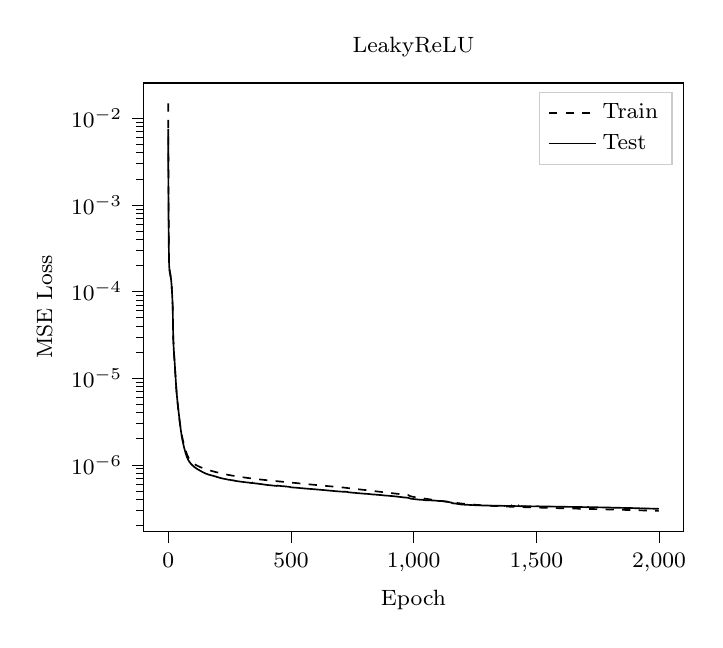
\begin{tikzpicture}

\begin{axis}[
legend cell align={left},
legend style={fill opacity=0.8, draw opacity=1, text opacity=1, draw=white!80!black},
log basis y={10},
tick align=outside,
tick pos=left,
title={LeakyReLU},
x grid style={white!69.0196078431373!black},
xlabel={Epoch},
xmin=-99.95, xmax=2098.95,
xtick style={color=black},
y grid style={white!69.0196078431373!black},
ylabel={MSE Loss},
ymin=1.70791572547231e-07, ymax=0.0255488360607333,
ymode=log,
ytick style={color=black}
]
\addplot [semithick, black, dashed]
table {%
0 0.0148644272387028
1 0.00333734963089228
2 0.000750602022744715
3 0.000331206021597609
4 0.000207027630618541
5 0.000178633672956494
6 0.000169817901289207
7 0.000163992511370452
8 0.000158428034461394
9 0.000152649684350763
10 0.00014641946539632
11 0.000139678969775559
12 0.000132290519177332
13 0.000124130066971702
14 0.000115090908722777
15 0.000105129859155568
16 9.44059219655173e-05
17 8.3223627305415e-05
18 7.19209145499917e-05
19 5.9600600565318e-05
20 3.97648699054116e-05
21 2.79329969580431e-05
22 2.30094661437761e-05
23 2.03421610876831e-05
24 1.84593141466394e-05
25 1.68413770406914e-05
26 1.53453861585149e-05
27 1.39403166676857e-05
28 1.26229516022249e-05
29 1.13995978695129e-05
30 1.02803903319e-05
31 9.27881336542669e-06
32 8.39881708566281e-06
33 7.63946547408523e-06
34 6.99144020211406e-06
35 6.44443027772468e-06
36 5.98577112725707e-06
37 5.59156097597224e-06
38 5.24542606149225e-06
39 4.93420651258703e-06
40 4.64607294458119e-06
41 4.3748265293857e-06
42 4.12039487252969e-06
43 3.8861643104724e-06
44 3.67260006765946e-06
45 3.47844123746199e-06
46 3.30225424215769e-06
47 3.13898743047503e-06
48 2.98947314900033e-06
49 2.85182592716637e-06
50 2.72762016362549e-06
51 2.61402293841684e-06
52 2.5099930834358e-06
53 2.4150706948376e-06
54 2.32725503445863e-06
55 2.24705749849363e-06
56 2.17294952142311e-06
57 2.1049157987818e-06
58 2.04128094503631e-06
59 1.98188082879369e-06
60 1.92642735390791e-06
61 1.87334052122878e-06
62 1.8232318035416e-06
63 1.77455488795886e-06
64 1.72895183959554e-06
65 1.6861234399812e-06
66 1.64616296456188e-06
67 1.60743973128774e-06
68 1.57055133320227e-06
69 1.53456863944257e-06
70 1.50125948277946e-06
71 1.46981972636695e-06
72 1.44026260474561e-06
73 1.41147857323176e-06
74 1.38520127060815e-06
75 1.36031598432851e-06
76 1.33676044734443e-06
77 1.3148170181978e-06
78 1.29389646752998e-06
79 1.27433537693378e-06
80 1.25646557970072e-06
81 1.2384471808673e-06
82 1.22196116879536e-06
83 1.20638403507201e-06
84 1.19190501561661e-06
85 1.17844780726273e-06
86 1.16571712385394e-06
87 1.1539444496691e-06
88 1.14418008098482e-06
89 1.13371917686322e-06
90 1.12408099414552e-06
91 1.1148123342366e-06
92 1.10610182443338e-06
93 1.09807221093661e-06
94 1.09074505050444e-06
95 1.0839480192999e-06
96 1.07734048407337e-06
97 1.07122849982488e-06
98 1.06452712140026e-06
99 1.05868495271011e-06
100 1.05291415113129e-06
101 1.04752679743569e-06
102 1.04214536537484e-06
103 1.0370281889891e-06
104 1.032027342319e-06
105 1.02744560464885e-06
106 1.02279366436164e-06
107 1.01820316623957e-06
108 1.01401851819105e-06
109 1.00975107895351e-06
110 1.0057904348173e-06
111 1.00208405191893e-06
112 9.98241210339756e-07
113 9.94370888776075e-07
114 9.90925482227567e-07
115 9.87395259301138e-07
116 9.83861367387817e-07
117 9.80596522055066e-07
118 9.77371847994846e-07
119 9.74262288309546e-07
120 9.71295058008082e-07
121 9.6826150081597e-07
122 9.6523639768975e-07
123 9.62448905852398e-07
124 9.59402455919189e-07
125 9.56513887700794e-07
126 9.53868651834e-07
127 9.51033602575535e-07
128 9.48263187240173e-07
129 9.45597496013306e-07
130 9.42952355558191e-07
131 9.40403254958255e-07
132 9.37919000818965e-07
133 9.35487815553415e-07
134 9.33048935337411e-07
135 9.30687048224854e-07
136 9.28267845239361e-07
137 9.25884347481087e-07
138 9.23637938910815e-07
139 9.21227984548523e-07
140 9.18846620891145e-07
141 9.16484609831514e-07
142 9.14296656503666e-07
143 9.12058346074218e-07
144 9.09871440057941e-07
145 9.07786169506153e-07
146 9.05647660886189e-07
147 9.03635627963695e-07
148 9.01687872357115e-07
149 8.9950875153022e-07
150 8.97521426622916e-07
151 8.95521069111282e-07
152 8.93521177772527e-07
153 8.91522843943449e-07
154 8.89579697087584e-07
155 8.87620785334775e-07
156 8.85896789583285e-07
157 8.83988975402872e-07
158 8.82208881847646e-07
159 8.80398930121373e-07
160 8.78538994015798e-07
161 8.76403134441262e-07
162 8.7463463688664e-07
163 8.72705812355434e-07
164 8.70566312670462e-07
165 8.68765719644671e-07
166 8.67004338203969e-07
167 8.653048454903e-07
168 8.63512691211099e-07
169 8.61854937170392e-07
170 8.60151822223543e-07
171 8.58458075072122e-07
172 8.56818996624043e-07
173 8.55136690688596e-07
174 8.53585893565878e-07
175 8.5187854273272e-07
176 8.50357727699702e-07
177 8.48755360294717e-07
178 8.47190044481749e-07
179 8.45670013589483e-07
180 8.44131327013997e-07
181 8.42642410887606e-07
182 8.41175444946884e-07
183 8.39656288363244e-07
184 8.38167764982245e-07
185 8.36532800619239e-07
186 8.35078147304102e-07
187 8.33758716908051e-07
188 8.32371983960911e-07
189 8.30889671789237e-07
190 8.29568857710683e-07
191 8.28064573511256e-07
192 8.26631372348174e-07
193 8.25454969628936e-07
194 8.24060114283043e-07
195 8.22638993369651e-07
196 8.2126220449652e-07
197 8.19915930264869e-07
198 8.20267484073156e-07
199 8.18703642607943e-07
200 8.17248432568363e-07
201 8.15823900992996e-07
202 8.14442585394204e-07
203 8.13095293437982e-07
204 8.11669069307186e-07
205 8.10307857349812e-07
206 8.09004709736882e-07
207 8.07590666070723e-07
208 8.06252364142779e-07
209 8.04654392212001e-07
210 8.0335848272739e-07
211 8.02302690658507e-07
212 8.00962444145625e-07
213 7.99703646720218e-07
214 7.98452317255283e-07
215 7.97217591738786e-07
216 7.96002158963915e-07
217 7.9481069326448e-07
218 7.93627711118461e-07
219 7.92467858858004e-07
220 7.91300207737322e-07
221 7.90077528890265e-07
222 7.88920517678093e-07
223 7.87720634576772e-07
224 7.86578616626343e-07
225 7.85441414691945e-07
226 7.84363267499089e-07
227 7.83269696910338e-07
228 7.82192492366107e-07
229 7.81227263516371e-07
230 7.80163437795522e-07
231 7.79063238198319e-07
232 7.78027706374473e-07
233 7.76964129954649e-07
234 7.75930989362905e-07
235 7.74893729442283e-07
236 7.73837977973813e-07
237 7.72835657613768e-07
238 7.71838034495431e-07
239 7.70846074615861e-07
240 7.69821481426902e-07
241 7.68822976212391e-07
242 7.67821201534957e-07
243 7.66846018862566e-07
244 7.65887867913762e-07
245 7.64930361214056e-07
246 7.63921686242952e-07
247 7.63010957257393e-07
248 7.62070085571054e-07
249 7.61139531945787e-07
250 7.60420157376984e-07
251 7.59426636150806e-07
252 7.58426511922039e-07
253 7.57507968302207e-07
254 7.56569720863354e-07
255 7.55625533727766e-07
256 7.54756878393437e-07
257 7.53833237837398e-07
258 7.52968338730398e-07
259 7.52147672017145e-07
260 7.51202681499308e-07
261 7.50205559867823e-07
262 7.4943015475526e-07
263 7.48610954261153e-07
264 7.47677468453389e-07
265 7.46997857405063e-07
266 7.46052829256882e-07
267 7.45165411899507e-07
268 7.44340018613343e-07
269 7.43665318836406e-07
270 7.42747071726058e-07
271 7.4204888295526e-07
272 7.41131473191103e-07
273 7.40440178674362e-07
274 7.39578193176271e-07
275 7.3881461977976e-07
276 7.37799187660926e-07
277 7.37035187341917e-07
278 7.36253217098692e-07
279 7.35415127010697e-07
280 7.34686662354989e-07
281 7.33878230974483e-07
282 7.33114714989824e-07
283 7.32347263181055e-07
284 7.31621643978997e-07
285 7.30857068063529e-07
286 7.30129704550109e-07
287 7.29444917936917e-07
288 7.28688947859268e-07
289 7.28014880451156e-07
290 7.27137706519443e-07
291 7.2640715151806e-07
292 7.25708816418091e-07
293 7.25009155303269e-07
294 7.24293989392777e-07
295 7.23561567397724e-07
296 7.2286156442658e-07
297 7.22185449788526e-07
298 7.21465641959185e-07
299 7.20789148289214e-07
300 7.20108953458976e-07
301 7.19449026178154e-07
302 7.18764739445987e-07
303 7.18094917701251e-07
304 7.17464760171538e-07
305 7.16808219209497e-07
306 7.16184726542224e-07
307 7.15528395758724e-07
308 7.14873352649192e-07
309 7.14168571732898e-07
310 7.13574344160861e-07
311 7.1287063936154e-07
312 7.12281224224398e-07
313 7.11596599359154e-07
314 7.1101726477707e-07
315 7.10344048059142e-07
316 7.09744001042623e-07
317 7.09173813802977e-07
318 7.08501808716733e-07
319 7.07896837610633e-07
320 7.07197004814475e-07
321 7.06599812318132e-07
322 7.05917090755293e-07
323 7.05374840876516e-07
324 7.04819606951901e-07
325 7.04185838287685e-07
326 7.03570776934725e-07
327 7.02973159619091e-07
328 7.02457169694526e-07
329 7.01814170426474e-07
330 7.01159818504493e-07
331 7.00675139412965e-07
332 7.00100038670826e-07
333 6.9944516293674e-07
334 6.98911392788659e-07
335 6.98320728275803e-07
336 6.97682788128873e-07
337 6.97246098184223e-07
338 6.96686453053985e-07
339 6.96352869169914e-07
340 6.95526991592033e-07
341 6.9484590517277e-07
342 6.94304655056044e-07
343 6.9400206361081e-07
344 6.92970413965099e-07
345 6.93037260532492e-07
346 6.92013609636888e-07
347 6.91989935560855e-07
348 6.90816037362652e-07
349 6.9062005174203e-07
350 6.89722630539791e-07
351 6.89461848594419e-07
352 6.88598280333963e-07
353 6.88385519012513e-07
354 6.87496540834331e-07
355 6.87273249681653e-07
356 6.86344381364279e-07
357 6.85784922154653e-07
358 6.85309239756293e-07
359 6.8513359936162e-07
360 6.84244536785172e-07
361 6.84097153609287e-07
362 6.83162119059943e-07
363 6.82782644759072e-07
364 6.82589405883505e-07
365 6.8159318890082e-07
366 6.81068037124533e-07
367 6.80618575174208e-07
368 6.80053423749882e-07
369 6.79640693476813e-07
370 6.79050741510423e-07
371 6.78609955187426e-07
372 6.78057203842286e-07
373 6.77662977224713e-07
374 6.77112505997002e-07
375 6.76636222607385e-07
376 6.76250711990178e-07
377 6.75681376677062e-07
378 6.75209785029551e-07
379 6.74681991128523e-07
380 6.74513683136979e-07
381 6.73722616213013e-07
382 6.73302310929102e-07
383 6.72808587580676e-07
384 6.72407056214297e-07
385 6.71915421463609e-07
386 6.71427296765614e-07
387 6.71025953465687e-07
388 6.7049164735522e-07
389 6.70016919258387e-07
390 6.69557675067267e-07
391 6.69086867844726e-07
392 6.68597802928161e-07
393 6.68190762553422e-07
394 6.67692410345921e-07
395 6.67240023972226e-07
396 6.66790877019707e-07
397 6.66323490648324e-07
398 6.65903456606998e-07
399 6.65471397070405e-07
400 6.65007362329106e-07
401 6.64616963959475e-07
402 6.64189005348703e-07
403 6.63769749593257e-07
404 6.63356940961535e-07
405 6.62935873677384e-07
406 6.6251740221901e-07
407 6.62097921363625e-07
408 6.61683327294327e-07
409 6.61271375818728e-07
410 6.60858302936163e-07
411 6.60460645164562e-07
412 6.6005227745336e-07
413 6.59639243394849e-07
414 6.5922696452958e-07
415 6.58827367658432e-07
416 6.58425498315296e-07
417 6.5801929646625e-07
418 6.57625117895577e-07
419 6.57224236348952e-07
420 6.5661854195298e-07
421 6.56017475847648e-07
422 6.55518018916723e-07
423 6.55074278228085e-07
424 6.54699447096618e-07
425 6.54264191396692e-07
426 6.53816869700563e-07
427 6.53326964823009e-07
428 6.52873706030732e-07
429 6.52448715413811e-07
430 6.51987482811478e-07
431 6.51630326260033e-07
432 6.51166140116288e-07
433 6.50728281328838e-07
434 6.50352801045528e-07
435 6.49924126832957e-07
436 6.49520926629066e-07
437 6.49109188529451e-07
438 6.48725988511956e-07
439 6.48329360970479e-07
440 6.47936029650964e-07
441 6.47537012639532e-07
442 6.47503992468046e-07
443 6.47304684633809e-07
444 6.46791755926301e-07
445 6.46174046053716e-07
446 6.45631595219243e-07
447 6.45148015280483e-07
448 6.4464382931817e-07
449 6.44142668491554e-07
450 6.4371638593741e-07
451 6.4329291483034e-07
452 6.42818815379087e-07
453 6.4243620757054e-07
454 6.41965242266451e-07
455 6.41560947940434e-07
456 6.4108713894484e-07
457 6.40711664800619e-07
458 6.40245212196078e-07
459 6.39877146284107e-07
460 6.39416840158447e-07
461 6.38994611691146e-07
462 6.38533215393977e-07
463 6.38164307375177e-07
464 6.37705450529324e-07
465 6.37337720817754e-07
466 6.36884023322182e-07
467 6.36565714486892e-07
468 6.35994193231681e-07
469 6.35576846804042e-07
470 6.35110142454209e-07
471 6.34726450087442e-07
472 6.34274996968998e-07
473 6.33879317220476e-07
474 6.33418987760592e-07
475 6.33054129139055e-07
476 6.32558955913964e-07
477 6.32200792907156e-07
478 6.31757687600043e-07
479 6.31408914216536e-07
480 6.30983657273987e-07
481 6.30627516443383e-07
482 6.30192174881472e-07
483 6.29844393728263e-07
484 6.29409517699742e-07
485 6.29049891742284e-07
486 6.28630618265902e-07
487 6.28272145732467e-07
488 6.27843531489702e-07
489 6.27503492012238e-07
490 6.27080744209252e-07
491 6.26735475819373e-07
492 6.26306154430267e-07
493 6.25968398722421e-07
494 6.25546789720488e-07
495 6.25211958649174e-07
496 6.24788373372098e-07
497 6.24449280010708e-07
498 6.23962057133554e-07
499 6.23558213717956e-07
500 6.2311415599936e-07
501 6.22750209018363e-07
502 6.22350057199128e-07
503 6.21995929662944e-07
504 6.21580487475626e-07
505 6.21248701463628e-07
506 6.20837227202742e-07
507 6.20487857943885e-07
508 6.2008267529734e-07
509 6.19707906508893e-07
510 6.19289868623696e-07
511 6.18935109201857e-07
512 6.18535905800854e-07
513 6.18207967761464e-07
514 6.17810335668878e-07
515 6.17487754837498e-07
516 6.17048165693745e-07
517 6.16747607693924e-07
518 6.16425678529708e-07
519 6.16018937733998e-07
520 6.15564609120156e-07
521 6.15231403671146e-07
522 6.14803654485741e-07
523 6.14466882382203e-07
524 6.13926075146765e-07
525 6.13603320687162e-07
526 6.13164834007307e-07
527 6.12889333567068e-07
528 6.1244176531261e-07
529 6.12171113900217e-07
530 6.11737456409855e-07
531 6.11406537032622e-07
532 6.10991987372245e-07
533 6.10615803282144e-07
534 6.10182909497325e-07
535 6.09855354056776e-07
536 6.09413068900722e-07
537 6.09052085394524e-07
538 6.08653819512028e-07
539 6.08387478564509e-07
540 6.07961950962022e-07
541 6.07622395477847e-07
542 6.07195113218495e-07
543 6.06802663170924e-07
544 6.06362741748967e-07
545 6.06013731712096e-07
546 6.0559248045422e-07
547 6.05250503625143e-07
548 6.04716681607442e-07
549 6.04371584088881e-07
550 6.03937985829361e-07
551 6.03589404704508e-07
552 6.03148568060874e-07
553 6.02801457745272e-07
554 6.0235625136329e-07
555 6.01985544463446e-07
556 6.01539943161811e-07
557 6.01232765262694e-07
558 6.00807006364335e-07
559 6.00492180907963e-07
560 6.0005816808939e-07
561 5.99730774595741e-07
562 5.99223440019614e-07
563 5.98925630910685e-07
564 5.98511263632418e-07
565 5.98205809396291e-07
566 5.97765539339434e-07
567 5.97455265236135e-07
568 5.97010945085685e-07
569 5.9672484819373e-07
570 5.96299604083583e-07
571 5.96071399556308e-07
572 5.95513366789646e-07
573 5.95187032928379e-07
574 5.947183740318e-07
575 5.94433451610144e-07
576 5.93983866451708e-07
577 5.93703354780928e-07
578 5.93230489997154e-07
579 5.92965793160261e-07
580 5.92490404656587e-07
581 5.92217652197746e-07
582 5.9175461059624e-07
583 5.91483319766439e-07
584 5.91055219629766e-07
585 5.9077541931174e-07
586 5.90313007251098e-07
587 5.90037488734652e-07
588 5.89601683429919e-07
589 5.89313242372214e-07
590 5.88861738904711e-07
591 5.88606085244692e-07
592 5.88205910432293e-07
593 5.87919526992664e-07
594 5.8745086768397e-07
595 5.87203168748829e-07
596 5.86743687904345e-07
597 5.86504606161498e-07
598 5.86034405827718e-07
599 5.85759843318101e-07
600 5.85295431378086e-07
601 5.85048269172717e-07
602 5.84578794146751e-07
603 5.84336741496827e-07
604 5.83889424504491e-07
605 5.8371987589112e-07
606 5.83250819758518e-07
607 5.82936998782202e-07
608 5.82475648911895e-07
609 5.822194414975e-07
610 5.81760691360955e-07
611 5.81514034749375e-07
612 5.8107778048111e-07
613 5.80798643440517e-07
614 5.8034996423828e-07
615 5.8007643750102e-07
616 5.79669754557699e-07
617 5.79423551016589e-07
618 5.78947847898803e-07
619 5.7868813833295e-07
620 5.78234088450813e-07
621 5.77960293540514e-07
622 5.7753287774176e-07
623 5.77290330667779e-07
624 5.76830392489569e-07
625 5.76586579811078e-07
626 5.76101825032538e-07
627 5.75859893572783e-07
628 5.75397084972451e-07
629 5.75150781202183e-07
630 5.74713401903182e-07
631 5.7447310602754e-07
632 5.74012735526708e-07
633 5.73774994833798e-07
634 5.73327271069957e-07
635 5.73114834153898e-07
636 5.72660245197199e-07
637 5.7240989970353e-07
638 5.71956064860046e-07
639 5.71697264476256e-07
640 5.71240307664311e-07
641 5.70994088292309e-07
642 5.70539148810667e-07
643 5.70304007425193e-07
644 5.69833525858598e-07
645 5.69588442289159e-07
646 5.69132603871481e-07
647 5.68892071527216e-07
648 5.68438184046727e-07
649 5.68201071160956e-07
650 5.67769946428598e-07
651 5.67519301142738e-07
652 5.6707707179271e-07
653 5.66797595681123e-07
654 5.66352859991071e-07
655 5.66096162472718e-07
656 5.65686599273363e-07
657 5.65438366834314e-07
658 5.65017211897612e-07
659 5.64772737391195e-07
660 5.64293594010223e-07
661 5.64047870213358e-07
662 5.63645380410094e-07
663 5.63384342626705e-07
664 5.62980142362335e-07
665 5.62727795866635e-07
666 5.62271209290088e-07
667 5.62005503908836e-07
668 5.61633367738068e-07
669 5.61361019336459e-07
670 5.60907587512816e-07
671 5.60647555943206e-07
672 5.60207655595946e-07
673 5.59965208736912e-07
674 5.59675780166913e-07
675 5.59391941266085e-07
676 5.58971077055048e-07
677 5.58727743012355e-07
678 5.58255349702108e-07
679 5.5799404208301e-07
680 5.5754053700241e-07
681 5.57285783443717e-07
682 5.56846114776022e-07
683 5.56599550662895e-07
684 5.56152776738372e-07
685 5.55905638606191e-07
686 5.55450992109741e-07
687 5.55227351341614e-07
688 5.54761071512644e-07
689 5.54549272450799e-07
690 5.54089646058742e-07
691 5.53867962665322e-07
692 5.53422880528842e-07
693 5.5320079773935e-07
694 5.5274819114004e-07
695 5.52521287801255e-07
696 5.5206996151469e-07
697 5.51794728323784e-07
698 5.51397915060647e-07
699 5.5119633870504e-07
700 5.50707732926981e-07
701 5.50483585669781e-07
702 5.5005929785068e-07
703 5.49791805909194e-07
704 5.49363092531507e-07
705 5.49153537050984e-07
706 5.48734435838583e-07
707 5.48524624861102e-07
708 5.48033714892426e-07
709 5.47864530929587e-07
710 5.47407044180659e-07
711 5.47192967673027e-07
712 5.46663945314663e-07
713 5.46469165058738e-07
714 5.46026377676867e-07
715 5.45797743370713e-07
716 5.45408502446776e-07
717 5.45146161812227e-07
718 5.44686208826306e-07
719 5.4444843793533e-07
720 5.44042121731536e-07
721 5.44187411392727e-07
722 5.43547544765488e-07
723 5.42903439722409e-07
724 5.42304797178872e-07
725 5.41774102529757e-07
726 5.41298678271573e-07
727 5.40787423858546e-07
728 5.40312020774536e-07
729 5.39910445837677e-07
730 5.39371933314214e-07
731 5.39032324013533e-07
732 5.38397320511308e-07
733 5.38005847772638e-07
734 5.37580982125974e-07
735 5.37113240582698e-07
736 5.36665524890623e-07
737 5.3628786932336e-07
738 5.35821611535425e-07
739 5.3551504601046e-07
740 5.34989343293546e-07
741 5.34692306075613e-07
742 5.34238284117805e-07
743 5.33852620080211e-07
744 5.33480754000948e-07
745 5.33024487040734e-07
746 5.32662216912172e-07
747 5.32245440751922e-07
748 5.31847421598286e-07
749 5.31583600732688e-07
750 5.31042589130948e-07
751 5.30784487636993e-07
752 5.30310267848222e-07
753 5.30027119310716e-07
754 5.29521326086524e-07
755 5.29201154762404e-07
756 5.28709079290479e-07
757 5.28442658435324e-07
758 5.27953152186456e-07
759 5.27690907290435e-07
760 5.27205177448309e-07
761 5.26892414683289e-07
762 5.26405703695332e-07
763 5.26151932234598e-07
764 5.25638900228387e-07
765 5.2538255179968e-07
766 5.24913538470173e-07
767 5.24627415103396e-07
768 5.24143547863787e-07
769 5.23870203437582e-07
770 5.23359917082189e-07
771 5.23059499315082e-07
772 5.22546751852815e-07
773 5.22258667359665e-07
774 5.21781591501735e-07
775 5.21461515333499e-07
776 5.21047451144341e-07
777 5.20667105519124e-07
778 5.20264812351456e-07
779 5.19935537340643e-07
780 5.19469053031685e-07
781 5.19178764761818e-07
782 5.18717480986197e-07
783 5.18486472344648e-07
784 5.18063059260498e-07
785 5.1770965706055e-07
786 5.17317782481541e-07
787 5.17047028139928e-07
788 5.16598040718463e-07
789 5.16272202006007e-07
790 5.15890133598873e-07
791 5.1559194417905e-07
792 5.15092240675585e-07
793 5.14856525086316e-07
794 5.14366608740602e-07
795 5.14138488711069e-07
796 5.1369179050198e-07
797 5.133947706355e-07
798 5.1297357916269e-07
799 5.1269512967167e-07
800 5.12259364455758e-07
801 5.1196938757414e-07
802 5.11423140920897e-07
803 5.11186035765832e-07
804 5.108558257092e-07
805 5.10589589111987e-07
806 5.10150635591344e-07
807 5.09905413366596e-07
808 5.09488112413692e-07
809 5.0918477496964e-07
810 5.08788510359182e-07
811 5.08506359878424e-07
812 5.08111304810654e-07
813 5.07820337901421e-07
814 5.07405267313743e-07
815 5.07125847690304e-07
816 5.06688020934121e-07
817 5.06418203016779e-07
818 5.05994589261149e-07
819 5.05725315562699e-07
820 5.05358103424669e-07
821 5.05075605559568e-07
822 5.04433651911995e-07
823 5.04046690537052e-07
824 5.03614987664491e-07
825 5.03243534893727e-07
826 5.02741254081229e-07
827 5.02363778650761e-07
828 5.0181188987608e-07
829 5.01155536113629e-07
830 5.00639151781002e-07
831 5.00094774650961e-07
832 4.99718042917152e-07
833 4.99335891149144e-07
834 4.98984696335469e-07
835 4.98626764695587e-07
836 4.98176735277411e-07
837 4.97781516273221e-07
838 4.97396944084016e-07
839 4.97024179267669e-07
840 4.96623089802029e-07
841 4.9619203473128e-07
842 4.95837466530702e-07
843 4.95356492848487e-07
844 4.94947353985253e-07
845 4.94624493896367e-07
846 4.94189927721322e-07
847 4.93753210434988e-07
848 4.93364277460273e-07
849 4.93005060846485e-07
850 4.92574361317111e-07
851 4.92261623520562e-07
852 4.91839595838428e-07
853 4.91472612594634e-07
854 4.91078210103524e-07
855 4.90717624558101e-07
856 4.90344198198045e-07
857 4.89971666482347e-07
858 4.89575231455319e-07
859 4.89207917780732e-07
860 4.8886572173501e-07
861 4.88452469610934e-07
862 4.88092318505551e-07
863 4.87744442438043e-07
864 4.87433638966195e-07
865 4.87001789679198e-07
866 4.86642392530712e-07
867 4.86256370052729e-07
868 4.85970414203507e-07
869 4.85520277266005e-07
870 4.85194746914885e-07
871 4.84795060486931e-07
872 4.8450660469257e-07
873 4.84076300665492e-07
874 4.83778275267355e-07
875 4.83363721940577e-07
876 4.83014998721387e-07
877 4.82567401576262e-07
878 4.82165626024766e-07
879 4.81873086187079e-07
880 4.81442710679403e-07
881 4.81068505791882e-07
882 4.80751659097223e-07
883 4.80426024751068e-07
884 4.80023959966047e-07
885 4.796470899322e-07
886 4.79263505340555e-07
887 4.78941620059459e-07
888 4.78609426863841e-07
889 4.78185967480727e-07
890 4.77746801095691e-07
891 4.77495924258164e-07
892 4.77138562104074e-07
893 4.76734690607827e-07
894 4.76396770054066e-07
895 4.76033359916528e-07
896 4.75629839783664e-07
897 4.7529189306772e-07
898 4.75028509299591e-07
899 4.74598706588836e-07
900 4.74232805089514e-07
901 4.73863658129403e-07
902 4.73503784462537e-07
903 4.73214756993912e-07
904 4.72819625130683e-07
905 4.72471625627691e-07
906 4.72109106254948e-07
907 4.71858331579256e-07
908 4.71460500378384e-07
909 4.71170830238066e-07
910 4.70762764038568e-07
911 4.70420068552357e-07
912 4.70193007899411e-07
913 4.69732255297117e-07
914 4.69328430256155e-07
915 4.69008694636841e-07
916 4.68750404195362e-07
917 4.68294574801575e-07
918 4.67943003044979e-07
919 4.67603833413932e-07
920 4.6726228927696e-07
921 4.67024187202014e-07
922 4.66549970042252e-07
923 4.66196309801603e-07
924 4.65849686818842e-07
925 4.65657492441096e-07
926 4.6514172363743e-07
927 4.6484536051139e-07
928 4.64433631279348e-07
929 4.64285816306642e-07
930 4.63722799736388e-07
931 4.63393946745327e-07
932 4.63028061346904e-07
933 4.62868733578148e-07
934 4.62303378796491e-07
935 4.61944667279113e-07
936 4.61593672994809e-07
937 4.61465650644755e-07
938 4.60907661022247e-07
939 4.60600220463903e-07
940 4.6021002177099e-07
941 4.59943743535973e-07
942 4.59559822544975e-07
943 4.59191470767451e-07
944 4.58823429340782e-07
945 4.58568544715376e-07
946 4.58253700188038e-07
947 4.57775354860246e-07
948 4.57443201653973e-07
949 4.57248985242131e-07
950 4.56788529746177e-07
951 4.56413603274086e-07
952 4.56049293291017e-07
953 4.55718323721044e-07
954 4.55268215404203e-07
955 4.54996806922736e-07
956 4.54735002605844e-07
957 4.54331303615163e-07
958 4.53895254239001e-07
959 4.53565293838665e-07
960 4.53295954372379e-07
961 4.52920906539589e-07
962 4.52633616063736e-07
963 4.52290183702075e-07
964 4.51753988272685e-07
965 4.51526366362032e-07
966 4.51130627027396e-07
967 4.50771134154593e-07
968 4.504252864308e-07
969 4.50136636729326e-07
970 4.49762404599596e-07
971 4.4941030162704e-07
972 4.49197960506353e-07
973 4.48709193022978e-07
974 4.48431595785337e-07
975 4.48094398578291e-07
976 4.4774719881957e-07
977 4.47329700762111e-07
978 4.47107959246296e-07
979 4.45311586858566e-07
980 4.42267165908561e-07
981 4.41070118895937e-07
982 4.40142427535761e-07
983 4.39295067039325e-07
984 4.38643088358504e-07
985 4.36957642435232e-07
986 4.35593108733201e-07
987 4.34702707551082e-07
988 4.33474616400531e-07
989 4.32703829105208e-07
990 4.32289674321851e-07
991 4.31421487917305e-07
992 4.30638353520862e-07
993 4.29790937616303e-07
994 4.28880565337408e-07
995 4.28401135650347e-07
996 4.27787201346064e-07
997 4.27183281047405e-07
998 4.26694344852763e-07
999 4.2636703791743e-07
1000 4.25715062704057e-07
1001 4.25246964852022e-07
1002 4.24845545552444e-07
1003 4.24308888639757e-07
1004 4.23964489456807e-07
1005 4.23528313447719e-07
1006 4.22984388706027e-07
1007 4.225807735736e-07
1008 4.22272394018819e-07
1009 4.21754303317812e-07
1010 4.21508764347323e-07
1011 4.20943191883794e-07
1012 4.20336185086967e-07
1013 4.19858491000014e-07
1014 4.1939585513262e-07
1015 4.19118752247982e-07
1016 4.18458747006412e-07
1017 4.18054913723154e-07
1018 4.17623710319504e-07
1019 4.17345911756684e-07
1020 4.1684959707311e-07
1021 4.16479742753495e-07
1022 4.16232555934926e-07
1023 4.1558006725495e-07
1024 4.15228342362184e-07
1025 4.15229226916836e-07
1026 4.14557101422019e-07
1027 4.14188685837757e-07
1028 4.137652676377e-07
1029 4.13552009050022e-07
1030 4.13012748268216e-07
1031 4.12709136242029e-07
1032 4.12403044578014e-07
1033 4.12024662679755e-07
1034 4.11686833103886e-07
1035 4.11097062823274e-07
1036 4.11059944923409e-07
1037 4.10612124298382e-07
1038 4.10058860069284e-07
1039 4.09830215701845e-07
1040 4.09236865593243e-07
1041 4.08992037847611e-07
1042 4.08167432894402e-07
1043 4.07781641527549e-07
1044 4.07499990515703e-07
1045 4.06984923031928e-07
1046 4.06398309621636e-07
1047 4.06130208801869e-07
1048 4.05844250565224e-07
1049 4.05634460008741e-07
1050 4.05246325286157e-07
1051 4.04832696432322e-07
1052 4.04589275078138e-07
1053 4.04333232410181e-07
1054 4.0388796469415e-07
1055 4.0364550858385e-07
1056 4.03237107150289e-07
1057 4.02781264639884e-07
1058 4.02806778183162e-07
1059 4.01965887306233e-07
1060 4.01510594059573e-07
1061 4.00938951401031e-07
1062 4.00572816303679e-07
1063 4.00084503098697e-07
1064 3.99712360263038e-07
1065 3.99338280672623e-07
1066 3.98853183725123e-07
1067 3.98574016514885e-07
1068 3.98165261131567e-07
1069 3.9791169047021e-07
1070 3.97472268019783e-07
1071 3.97099917236687e-07
1072 3.96636626348368e-07
1073 3.96424626273983e-07
1074 3.96097346396118e-07
1075 3.9559541224321e-07
1076 3.95176014095e-07
1077 3.9485332503375e-07
1078 3.94414255026732e-07
1079 3.94210009147855e-07
1080 3.93897365086104e-07
1081 3.94073744161005e-07
1082 3.92707131538828e-07
1083 3.92443426818545e-07
1084 3.92263928972625e-07
1085 3.91811526995411e-07
1086 3.91438045383552e-07
1087 3.91222988042728e-07
1088 3.90767820931615e-07
1089 3.90392165115827e-07
1090 3.90058417949035e-07
1091 3.89737378512223e-07
1092 3.89416854545743e-07
1093 3.89117823701213e-07
1094 3.88820500631937e-07
1095 3.8860628005466e-07
1096 3.88284502861325e-07
1097 3.8773857590968e-07
1098 3.87415723963613e-07
1099 3.87093581963427e-07
1100 3.86819972547414e-07
1101 3.8655951644273e-07
1102 3.86174517572613e-07
1103 3.85863807807141e-07
1104 3.85488108648246e-07
1105 3.85170436189242e-07
1106 3.84719854892523e-07
1107 3.84718544239604e-07
1108 3.84024391522075e-07
1109 3.83650835544813e-07
1110 3.83382792236375e-07
1111 3.83040656402045e-07
1112 3.82753346201525e-07
1113 3.82416109658834e-07
1114 3.82373510092293e-07
1115 3.81928717573032e-07
1116 3.81812806622861e-07
1117 3.81203720849044e-07
1118 3.80974276083634e-07
1119 3.80499999522499e-07
1120 3.80254684600345e-07
1121 3.7986570839621e-07
1122 3.79738977585475e-07
1123 3.79311346222266e-07
1124 3.79113227651828e-07
1125 3.7877028913158e-07
1126 3.7836112139189e-07
1127 3.77982800344512e-07
1128 3.78119575884739e-07
1129 3.77618890752274e-07
1130 3.77162941205711e-07
1131 3.7672415348311e-07
1132 3.76497530936604e-07
1133 3.76125739251165e-07
1134 3.76046060509339e-07
1135 3.75449260715754e-07
1136 3.75253203273473e-07
1137 3.74917057925472e-07
1138 3.74622404692104e-07
1139 3.7428821870833e-07
1140 3.74284405566527e-07
1141 3.7362211756431e-07
1142 3.73366226355643e-07
1143 3.7307717714441e-07
1144 3.72830825526194e-07
1145 3.72424451896336e-07
1146 3.72418132940311e-07
1147 3.7213091133026e-07
1148 3.71713215983505e-07
1149 3.71452914535553e-07
1150 3.71178188473209e-07
1151 3.70909355197568e-07
1152 3.7053996253178e-07
1153 3.7024783931372e-07
1154 3.69873657135145e-07
1155 3.69505103691381e-07
1156 3.69253701279604e-07
1157 3.68807387985726e-07
1158 3.68308296941677e-07
1159 3.68027352777744e-07
1160 3.67674302410137e-07
1161 3.67324845441885e-07
1162 3.67093079873371e-07
1163 3.66817634045447e-07
1164 3.66528322331305e-07
1165 3.66260036969379e-07
1166 3.65974232906296e-07
1167 3.6576783041653e-07
1168 3.65757778212128e-07
1169 3.65359265160237e-07
1170 3.64927529545866e-07
1171 3.64539682664144e-07
1172 3.64183218977132e-07
1173 3.63697715883404e-07
1174 3.63248774547742e-07
1175 3.6295745351822e-07
1176 3.62568556099063e-07
1177 3.62408816727111e-07
1178 3.61902688752025e-07
1179 3.61626319858033e-07
1180 3.61431617832864e-07
1181 3.61043409355943e-07
1182 3.60797934973789e-07
1183 3.60444958303674e-07
1184 3.60248958102716e-07
1185 3.59936896558111e-07
1186 3.59555476705964e-07
1187 3.59374415111802e-07
1188 3.58965990059801e-07
1189 3.58561037799632e-07
1190 3.58322259430111e-07
1191 3.57995596175442e-07
1192 3.57769069225355e-07
1193 3.57516862507623e-07
1194 3.57242059436658e-07
1195 3.57074874074215e-07
1196 3.56846210692652e-07
1197 3.56573667573912e-07
1198 3.56349139025269e-07
1199 3.56250705209504e-07
1200 3.55875810996054e-07
1201 3.55695545266599e-07
1202 3.55430612060559e-07
1203 3.55257044837742e-07
1204 3.55036958367805e-07
1205 3.54729504230988e-07
1206 3.54575795554979e-07
1207 3.54330831036975e-07
1208 3.54163805582175e-07
1209 3.53934707121084e-07
1210 3.53760961694149e-07
1211 3.53559004942383e-07
1212 3.53348837684564e-07
1213 3.53167481250694e-07
1214 3.52938252042634e-07
1215 3.52749994284807e-07
1216 3.52585982660969e-07
1217 3.52407975704239e-07
1218 3.52169507415567e-07
1219 3.51973961208785e-07
1220 3.51758787793699e-07
1221 3.51502807255599e-07
1222 3.51306851079869e-07
1223 3.51152501224306e-07
1224 3.50899278146244e-07
1225 3.50712421344213e-07
1226 3.50511307786405e-07
1227 3.50340402199834e-07
1228 3.50174203553877e-07
1229 3.49866230820339e-07
1230 3.49717217829948e-07
1231 3.49455526098552e-07
1232 3.49285141943767e-07
1233 3.49022042534841e-07
1234 3.48864000585536e-07
1235 3.48586736819811e-07
1236 3.48445087801963e-07
1237 3.4818345256582e-07
1238 3.4813231708597e-07
1239 3.48225087407172e-07
1240 3.47784275412266e-07
1241 3.47621228634409e-07
1242 3.47436047128724e-07
1243 3.47174164780029e-07
1244 3.4713033489453e-07
1245 3.46868865150896e-07
1246 3.46827497459401e-07
1247 3.46505921307028e-07
1248 3.46359151983222e-07
1249 3.46254663149637e-07
1250 3.45973173082825e-07
1251 3.45937462505219e-07
1252 3.45498902305508e-07
1253 3.45166767687033e-07
1254 3.44957258484158e-07
1255 3.44883514060257e-07
1256 3.44460587214712e-07
1257 3.44291111339601e-07
1258 3.44095388989274e-07
1259 3.43959172042219e-07
1260 3.43810874603889e-07
1261 3.43625585593088e-07
1262 3.4358059095041e-07
1263 3.43212996391173e-07
1264 3.43100552726128e-07
1265 3.43164890786341e-07
1266 3.42759536103188e-07
1267 3.42773568959842e-07
1268 3.42893875803441e-07
1269 3.42620055683085e-07
1270 3.4228207704956e-07
1271 3.42381971016437e-07
1272 3.42026907333093e-07
1273 3.41821995505143e-07
1274 3.41681918825998e-07
1275 3.41623348312226e-07
1276 3.41340164766279e-07
1277 3.41217368152513e-07
1278 3.4106308705617e-07
1279 3.40976784691804e-07
1280 3.4080946687709e-07
1281 3.40802128683038e-07
1282 3.40702538146331e-07
1283 3.40402227969605e-07
1284 3.40182375417442e-07
1285 3.40091809910348e-07
1286 3.39915428099857e-07
1287 3.39853421358782e-07
1288 3.39670542125248e-07
1289 3.39502068037234e-07
1290 3.39417640304873e-07
1291 3.39291082688931e-07
1292 3.39082802483404e-07
1293 3.39148367032749e-07
1294 3.38892482638187e-07
1295 3.38829270653207e-07
1296 3.38648870496172e-07
1297 3.38687307959162e-07
1298 3.38240516690291e-07
1299 3.38366272508495e-07
1300 3.38001319256875e-07
1301 3.37920434652972e-07
1302 3.37841576858011e-07
1303 3.37823672431625e-07
1304 3.3753024310812e-07
1305 3.37429006513901e-07
1306 3.37313680958573e-07
1307 3.37218410713547e-07
1308 3.3711456779173e-07
1309 3.36903703832547e-07
1310 3.36891655976501e-07
1311 3.36800533723647e-07
1312 3.3659107230477e-07
1313 3.36524350629475e-07
1314 3.36588194052467e-07
1315 3.3621560381647e-07
1316 3.36227974422343e-07
1317 3.35964050691473e-07
1318 3.3590479741008e-07
1319 3.35959069197145e-07
1320 3.3563762396227e-07
1321 3.3570893973689e-07
1322 3.35404225104696e-07
1323 3.35420296941891e-07
1324 3.35310365571218e-07
1325 3.35162345130868e-07
1326 3.35112290805739e-07
1327 3.35035934234895e-07
1328 3.34863490358828e-07
1329 3.3453481590584e-07
1330 3.34560684706275e-07
1331 3.34415690289802e-07
1332 3.34436880429223e-07
1333 3.34342135964505e-07
1334 3.3411748800205e-07
1335 3.33874048642713e-07
1336 3.33887440966407e-07
1337 3.33762760767797e-07
1338 3.33557971053722e-07
1339 3.33469831780064e-07
1340 3.333395412497e-07
1341 3.33323065277114e-07
1342 3.33160623696926e-07
1343 3.33146326468636e-07
1344 3.32997630756893e-07
1345 3.32955995787643e-07
1346 3.32814051603236e-07
1347 3.3281026241383e-07
1348 3.32498229099087e-07
1349 3.32466849641833e-07
1350 3.32391293376588e-07
1351 3.32259941842494e-07
1352 3.32225231424843e-07
1353 3.32077841072476e-07
1354 3.32005728822082e-07
1355 3.31841624657159e-07
1356 3.31928920083158e-07
1357 3.31696651336699e-07
1358 3.31594936319846e-07
1359 3.31512106100718e-07
1360 3.31501672782508e-07
1361 3.31306970345224e-07
1362 3.31109461292556e-07
1363 3.31097948134129e-07
1364 3.30970878607673e-07
1365 3.30980586127794e-07
1366 3.30741880006258e-07
1367 3.30851606676674e-07
1368 3.30796594830929e-07
1369 3.30699608035445e-07
1370 3.30719720835759e-07
1371 3.30387201159965e-07
1372 3.30450337429511e-07
1373 3.30311810436967e-07
1374 3.30153512820175e-07
1375 3.30106311636769e-07
1376 3.29856312781374e-07
1377 3.29988769316003e-07
1378 3.29781705133314e-07
1379 3.29643474735519e-07
1380 3.29575802702209e-07
1381 3.29661901908196e-07
1382 3.29384446779102e-07
1383 3.29194402652888e-07
1384 3.29174147502442e-07
1385 3.2892577434751e-07
1386 3.28936768760002e-07
1387 3.28938984807792e-07
1388 3.28622693380964e-07
1389 3.28631047203487e-07
1390 3.28663743040636e-07
1391 3.28427028435385e-07
1392 3.28422970120812e-07
1393 3.28242727945849e-07
1394 3.28273688822378e-07
1395 3.28060710437228e-07
1396 3.28181209752643e-07
1397 3.27843347669443e-07
1398 3.27852344064183e-07
1399 3.2829578710647e-07
1400 3.28064131871031e-07
1401 3.27575198873831e-07
1402 3.27536251177207e-07
1403 3.27420939470358e-07
1404 3.2741662860758e-07
1405 3.27226250057322e-07
1406 3.27265470950522e-07
1407 3.27060519509814e-07
1408 3.27155963816494e-07
1409 3.26972195878739e-07
1410 3.26970149174599e-07
1411 3.26863787329046e-07
1412 3.26782263279313e-07
1413 3.26663281526862e-07
1414 3.26726319926252e-07
1415 3.26526487675949e-07
1416 3.26492149575586e-07
1417 3.26372519289464e-07
1418 3.26526134919902e-07
1419 3.26281027753339e-07
1420 3.26192927850855e-07
1421 3.26291698719672e-07
1422 3.26084324228759e-07
1423 3.26008133122002e-07
1424 3.25901496594838e-07
1425 3.25920014496717e-07
1426 3.25827025420722e-07
1427 3.25687300644972e-07
1428 3.26062531392779e-07
1429 3.25628018437385e-07
1430 3.2562565948524e-07
1431 3.25352808538071e-07
1432 3.25273427925765e-07
1433 3.25321335537865e-07
1434 3.25138781853695e-07
1435 3.25163706605736e-07
1436 3.25108598367763e-07
1437 3.24951548883234e-07
1438 3.24962143700702e-07
1439 3.24829615223621e-07
1440 3.25090830237684e-07
1441 3.24795452463889e-07
1442 3.24721973001374e-07
1443 3.24631089085869e-07
1444 3.2456479630838e-07
1445 3.24642600965319e-07
1446 3.24464752360143e-07
1447 3.24280949101308e-07
1448 3.24287003877544e-07
1449 3.24112054428838e-07
1450 3.24111770346747e-07
1451 3.24085712215094e-07
1452 3.24007598564435e-07
1453 3.23942609085748e-07
1454 3.2425689070692e-07
1455 3.24005999075894e-07
1456 3.2361437681061e-07
1457 3.23674683443187e-07
1458 3.2351173168621e-07
1459 3.23458068230309e-07
1460 3.23479223787615e-07
1461 3.23319206508188e-07
1462 3.23341757123785e-07
1463 3.23198218914911e-07
1464 3.23270411364263e-07
1465 3.23068304957985e-07
1466 3.23069969759615e-07
1467 3.23080898247952e-07
1468 3.22920393280413e-07
1469 3.22857342759164e-07
1470 3.22821105278592e-07
1471 3.22736950657543e-07
1472 3.22708666047333e-07
1473 3.22561187388715e-07
1474 3.2244668971515e-07
1475 3.22537584629856e-07
1476 3.2234767521544e-07
1477 3.22275564869301e-07
1478 3.22260968928845e-07
1479 3.22126612921636e-07
1480 3.22229529807316e-07
1481 3.22072553345265e-07
1482 3.21982909795793e-07
1483 3.22065536110472e-07
1484 3.21898457372072e-07
1485 3.21896749035488e-07
1486 3.21722710658889e-07
1487 3.21782155673134e-07
1488 3.21655857334235e-07
1489 3.21540387943742e-07
1490 3.21610780446235e-07
1491 3.21390835281932e-07
1492 3.21524363023684e-07
1493 3.2131500721988e-07
1494 3.21355409518276e-07
1495 3.21366403952084e-07
1496 3.2123143392937e-07
1497 3.21120906043859e-07
1498 3.21158807956579e-07
1499 3.21153666938301e-07
1500 3.20950832460198e-07
1501 3.20903004755735e-07
1502 3.20872954738149e-07
1503 3.20826174515787e-07
1504 3.20889407738889e-07
1505 3.20691754176039e-07
1506 3.20632478270966e-07
1507 3.20689533992891e-07
1508 3.20531748741359e-07
1509 3.20420759095441e-07
1510 3.20409114671349e-07
1511 3.20266171875971e-07
1512 3.20465706288076e-07
1513 3.20110148116726e-07
1514 3.20114583416853e-07
1515 3.20165127867256e-07
1516 3.19939939579683e-07
1517 3.19961420586878e-07
1518 3.19884608479981e-07
1519 3.19850591942838e-07
1520 3.19754192247501e-07
1521 3.19659825549934e-07
1522 3.19542471565626e-07
1523 3.19522271233552e-07
1524 3.1952513759137e-07
1525 3.19442034466988e-07
1526 3.19308484826308e-07
1527 3.1926437686991e-07
1528 3.19322454409132e-07
1529 3.19090354508944e-07
1530 3.1914903206598e-07
1531 3.19048935295996e-07
1532 3.18985352343759e-07
1533 3.18868792234639e-07
1534 3.18823600416351e-07
1535 3.18969249775591e-07
1536 3.18667938614681e-07
1537 3.18681215368599e-07
1538 3.18583031408082e-07
1539 3.18604212985463e-07
1540 3.18418979318835e-07
1541 3.1837250921285e-07
1542 3.18446168733999e-07
1543 3.18235732798655e-07
1544 3.1822591738262e-07
1545 3.18200680894165e-07
1546 3.1824155977489e-07
1547 3.18066145119644e-07
1548 3.17969742788193e-07
1549 3.18165659486169e-07
1550 3.17947992201084e-07
1551 3.17837663196485e-07
1552 3.17799422937526e-07
1553 3.17749503373932e-07
1554 3.17725981943795e-07
1555 3.17654856075933e-07
1556 3.1745046170073e-07
1557 3.17432104033344e-07
1558 3.17421537815221e-07
1559 3.17527532082806e-07
1560 3.17331122076325e-07
1561 3.1720363658394e-07
1562 3.17183404767718e-07
1563 3.17158790586802e-07
1564 3.17055461529492e-07
1565 3.16942562001543e-07
1566 3.17018796096136e-07
1567 3.16961415805395e-07
1568 3.16822705308084e-07
1569 3.1673548660649e-07
1570 3.1669173003479e-07
1571 3.16677336762439e-07
1572 3.16670457948476e-07
1573 3.16591517567133e-07
1574 3.16468353531718e-07
1575 3.1647522484235e-07
1576 3.16485809719325e-07
1577 3.16312855744627e-07
1578 3.16247700645533e-07
1579 3.16220362343245e-07
1580 3.16188260690353e-07
1581 3.16109383760477e-07
1582 3.16156887059549e-07
1583 3.16068575635597e-07
1584 3.15873102728403e-07
1585 3.15975026701665e-07
1586 3.15779102422198e-07
1587 3.15815761297245e-07
1588 3.15671033362719e-07
1589 3.15747237223718e-07
1590 3.15594334843183e-07
1591 3.15574065240298e-07
1592 3.15509907693468e-07
1593 3.15438409678848e-07
1594 3.15528669297294e-07
1595 3.15281006912471e-07
1596 3.15268012819558e-07
1597 3.15299097358945e-07
1598 3.15124351033091e-07
1599 3.15032143682004e-07
1600 3.14968358829049e-07
1601 3.15165431196363e-07
1602 3.14933268924733e-07
1603 3.14842066984511e-07
1604 3.14790559968969e-07
1605 3.14805405700724e-07
1606 3.14614502052279e-07
1607 3.14726759292228e-07
1608 3.14509374746308e-07
1609 3.14674117142033e-07
1610 3.14487810229025e-07
1611 3.14573937380658e-07
1612 3.14394223408954e-07
1613 3.14384523349531e-07
1614 3.14405950419427e-07
1615 3.14362090051645e-07
1616 3.14184010818508e-07
1617 3.14153501655312e-07
1618 3.14043581461476e-07
1619 3.14059152806578e-07
1620 3.13894354967204e-07
1621 3.14038598588695e-07
1622 3.14356346699185e-07
1623 3.14293879981165e-07
1624 3.14200238548779e-07
1625 3.14175397726046e-07
1626 3.13871269945309e-07
1627 3.1394368009785e-07
1628 3.13715297558304e-07
1629 3.1380694633043e-07
1630 3.13606534241728e-07
1631 3.13643690411425e-07
1632 3.13666378573885e-07
1633 3.13586880650973e-07
1634 3.13423190370088e-07
1635 3.13455884217717e-07
1636 3.13332078007988e-07
1637 3.13316120802654e-07
1638 3.13285314419431e-07
1639 3.13249966531259e-07
1640 3.13080791741527e-07
1641 3.13154238334334e-07
1642 3.12935718767449e-07
1643 3.13037454141352e-07
1644 3.12864478829056e-07
1645 3.12887611663371e-07
1646 3.12814163436315e-07
1647 3.12779923319795e-07
1648 3.12677243989867e-07
1649 3.12674668265345e-07
1650 3.12483081728487e-07
1651 3.13008835682638e-07
1652 3.12390567842158e-07
1653 3.12456071270617e-07
1654 3.1229574748437e-07
1655 3.12338921325761e-07
1656 3.12201615948027e-07
1657 3.12339854595223e-07
1658 3.12096956406549e-07
1659 3.12131471773114e-07
1660 3.11996117972058e-07
1661 3.12029497557376e-07
1662 3.11892367115263e-07
1663 3.12013563373625e-07
1664 3.11821396117296e-07
1665 3.11737066255091e-07
1666 3.11751752903433e-07
1667 3.11542458518943e-07
1668 3.11465470417716e-07
1669 3.11640546655667e-07
1670 3.11447121475794e-07
1671 3.113907667327e-07
1672 3.1128856271323e-07
1673 3.1143680404e-07
1674 3.11213553068512e-07
1675 3.11212113537351e-07
1676 3.11191033297575e-07
1677 3.11144864852508e-07
1678 3.11065440115499e-07
1679 3.11046119790603e-07
1680 3.10867254668779e-07
1681 3.11016560125665e-07
1682 3.10783246312951e-07
1683 3.10997557086523e-07
1684 3.10670550469183e-07
1685 3.10749519698561e-07
1686 3.10596976952127e-07
1687 3.10744832269449e-07
1688 3.10395399182539e-07
1689 3.10655381646541e-07
1690 3.10417983520495e-07
1691 3.10629784621597e-07
1692 3.10311370782301e-07
1693 3.1037526576938e-07
1694 3.10243405010624e-07
1695 3.10281405603519e-07
1696 3.10096623323375e-07
1697 3.10194989395995e-07
1698 3.10098258829328e-07
1699 3.10130593128122e-07
1700 3.09984979040223e-07
1701 3.09938632540252e-07
1702 3.09827980473187e-07
1703 3.09812695462597e-07
1704 3.096528067843e-07
1705 3.09828499311493e-07
1706 3.09625381632372e-07
1707 3.09750097500228e-07
1708 3.09600050115932e-07
1709 3.09845477801218e-07
1710 3.09658715913486e-07
1711 3.09539044295093e-07
1712 3.09400075131805e-07
1713 3.09725576833841e-07
1714 3.0916625053834e-07
1715 3.09483384377529e-07
1716 3.09334076376899e-07
1717 3.0918433626681e-07
1718 3.09062954308104e-07
1719 3.09123950380297e-07
1720 3.08976081434764e-07
1721 3.091337238601e-07
1722 3.08965229287139e-07
1723 3.09116053983871e-07
1724 3.08689637293469e-07
1725 3.08736328939574e-07
1726 3.08669552644858e-07
1727 3.08603466613988e-07
1728 3.08530398037021e-07
1729 3.08627115401805e-07
1730 3.08540636936527e-07
1731 3.08427530285371e-07
1732 3.08334022712131e-07
1733 3.08257495653663e-07
1734 3.08236750498736e-07
1735 3.0833639345218e-07
1736 3.08096456222984e-07
1737 3.08075279455977e-07
1738 3.08042506972583e-07
1739 3.08085389832513e-07
1740 3.07968706749762e-07
1741 3.07898931581008e-07
1742 3.07764628203699e-07
1743 3.07773813283063e-07
1744 3.07717376465177e-07
1745 3.07653958117271e-07
1746 3.0765865913196e-07
1747 3.07626101644587e-07
1748 3.07552278009382e-07
1749 3.0735350994604e-07
1750 3.07628058081377e-07
1751 3.07336489342447e-07
1752 3.07368682385345e-07
1753 3.07209660846297e-07
1754 3.07406639642238e-07
1755 3.0710762363384e-07
1756 3.07180690796827e-07
1757 3.06997296227962e-07
1758 3.07280588238257e-07
1759 3.06843731650019e-07
1760 3.06940378493437e-07
1761 3.06794261831556e-07
1762 3.06837595772436e-07
1763 3.06610467816881e-07
1764 3.06829234347106e-07
1765 3.06454595275341e-07
1766 3.06707944893958e-07
1767 3.06326688800596e-07
1768 3.06441866172236e-07
1769 3.06257395521925e-07
1770 3.0633805037894e-07
1771 3.06157528299877e-07
1772 3.06200772897114e-07
1773 3.0607316737985e-07
1774 3.06098561296153e-07
1775 3.06194833605389e-07
1776 3.06072450797501e-07
1777 3.06052589152728e-07
1778 3.0598369404089e-07
1779 3.05753781354667e-07
1780 3.05756770544008e-07
1781 3.05665897727181e-07
1782 3.05728093714208e-07
1783 3.05646801621151e-07
1784 3.05738369860364e-07
1785 3.05382987974667e-07
1786 3.05652452290417e-07
1787 3.0544395694676e-07
1788 3.05572961565304e-07
1789 3.05190016284484e-07
1790 3.05378717335714e-07
1791 3.05075413500333e-07
1792 3.05183546778665e-07
1793 3.05088814037902e-07
1794 3.05365793757062e-07
1795 3.05033719747883e-07
1796 3.05069139692193e-07
1797 3.04773875001274e-07
1798 3.04957178123288e-07
1799 3.04655040785917e-07
1800 3.04872247021137e-07
1801 3.04794242460105e-07
1802 3.04774771770155e-07
1803 3.04634256494296e-07
1804 3.046867968024e-07
1805 3.04623855846842e-07
1806 3.04478786084417e-07
1807 3.04440137668394e-07
1808 3.04489119187679e-07
1809 3.04337516880082e-07
1810 3.0426601318112e-07
1811 3.04229888918428e-07
1812 3.04097428177386e-07
1813 3.04338748520649e-07
1814 3.04042303426399e-07
1815 3.04046707569228e-07
1816 3.03893465911642e-07
1817 3.04108458379915e-07
1818 3.03728165427231e-07
1819 3.04069386402261e-07
1820 3.03660852303267e-07
1821 3.03650683463275e-07
1822 3.03544722548565e-07
1823 3.03597130113076e-07
1824 3.03506354299543e-07
1825 3.03322645812898e-07
1826 3.03617171937276e-07
1827 3.03360720117496e-07
1828 3.03249289061114e-07
1829 3.03108788607176e-07
1830 3.03273794429515e-07
1831 3.02977811173832e-07
1832 3.03072520843273e-07
1833 3.03012808892333e-07
1834 3.02839288991663e-07
1835 3.02869932504279e-07
1836 3.02772856940692e-07
1837 3.02604050183675e-07
1838 3.02785141101936e-07
1839 3.02697704505306e-07
1840 3.02647801603939e-07
1841 3.02386721486414e-07
1842 3.02443652245188e-07
1843 3.02288002671958e-07
1844 3.02339900542847e-07
1845 3.02194082941298e-07
1846 3.02256330741102e-07
1847 3.02109679132911e-07
1848 3.02255458365153e-07
1849 3.02030160554523e-07
1850 3.01960260415513e-07
1851 3.01962238040687e-07
1852 3.01846855450094e-07
1853 3.01791661499351e-07
1854 3.01770279023117e-07
1855 3.01849823351574e-07
1856 3.01669510847091e-07
1857 3.01545374682632e-07
1858 3.0151376973464e-07
1859 3.01416563644352e-07
1860 3.01456793536659e-07
1861 3.01289437224739e-07
1862 3.01354336748716e-07
1863 3.01205066875809e-07
1864 3.01245784264381e-07
1865 3.01109555174151e-07
1866 3.01183946696426e-07
1867 3.0100350952722e-07
1868 3.00976861971947e-07
1869 3.00884783449362e-07
1870 3.01047703374024e-07
1871 3.00773745493643e-07
1872 3.00733479228654e-07
1873 3.00692512261946e-07
1874 3.0063736996766e-07
1875 3.00572687713441e-07
1876 3.00503531029506e-07
1877 3.00603009335987e-07
1878 3.00401623185564e-07
1879 3.00343361367084e-07
1880 3.0032322746365e-07
1881 3.00249160275712e-07
1882 3.00184128789738e-07
1883 3.00211509483006e-07
1884 3.00067204264565e-07
1885 2.99960682831113e-07
1886 2.99978455828409e-07
1887 2.99902618976944e-07
1888 2.99820982888832e-07
1889 2.99946893044023e-07
1890 2.99692950321173e-07
1891 2.99725934681305e-07
1892 2.99663779735226e-07
1893 2.99518005547839e-07
1894 2.99473131434524e-07
1895 2.99465885760242e-07
1896 2.99575580086753e-07
1897 2.99349106128943e-07
1898 2.99262351035168e-07
1899 2.9926471443531e-07
1900 2.99133502601023e-07
1901 2.99155919819327e-07
1902 2.99006076474484e-07
1903 2.99133789390282e-07
1904 2.98925287424368e-07
1905 2.98941225764793e-07
1906 2.9879624715079e-07
1907 2.9895922090617e-07
1908 2.98671382864768e-07
1909 2.98679200191998e-07
1910 2.98591146808747e-07
1911 2.98603283383159e-07
1912 2.98482322143911e-07
1913 2.98465000426518e-07
1914 2.98486448997437e-07
1915 2.98328453361307e-07
1916 2.98258284743724e-07
1917 2.98272029993996e-07
1918 2.9815794463417e-07
1919 2.98116875256937e-07
1920 2.98200684603955e-07
1921 2.98044728452851e-07
1922 2.97941690746484e-07
1923 2.97912768431274e-07
1924 2.97862047318631e-07
1925 2.97789504678292e-07
1926 2.97767631202817e-07
1927 2.97833934823188e-07
1928 2.97641517363445e-07
1929 2.97627088585273e-07
1930 2.97398515307634e-07
1931 2.97637071803081e-07
1932 2.97316301185901e-07
1933 2.9743815220229e-07
1934 2.97396039492526e-07
1935 2.97155774788394e-07
1936 2.972102788803e-07
1937 2.97290856764221e-07
1938 2.97404336421891e-07
1939 2.97170349625731e-07
1940 2.97167980377822e-07
1941 2.97099185310401e-07
1942 2.9688234484837e-07
1943 2.96936517749202e-07
1944 2.96624542492907e-07
1945 2.97014116000582e-07
1946 2.96760317269218e-07
1947 2.96771138536656e-07
1948 2.96515731449176e-07
1949 2.9663090040799e-07
1950 2.9657164558472e-07
1951 2.9648336685284e-07
1952 2.96345633593376e-07
1953 2.9631420408549e-07
1954 2.96308615659768e-07
1955 2.9610010748371e-07
1956 2.9626472518629e-07
1957 2.9594645059916e-07
1958 2.96222448795902e-07
1959 2.95816891757283e-07
1960 2.95940765774105e-07
1961 2.95927517129257e-07
1962 2.95857750273854e-07
1963 2.95589895799253e-07
1964 2.95722840512269e-07
1965 2.95564092198219e-07
1966 2.95687444705095e-07
1967 2.95598649046269e-07
1968 2.95281853446738e-07
1969 2.95426976748558e-07
1970 2.95280896850159e-07
1971 2.95339915290072e-07
1972 2.95072210619196e-07
1973 2.95270798041258e-07
1974 2.95314228253574e-07
1975 2.94874492254849e-07
1976 2.95091132208825e-07
1977 2.95017232964767e-07
1978 2.94680657525248e-07
1979 2.94926457868883e-07
1980 2.94877394068749e-07
1981 2.94727112077453e-07
1982 2.94783511044727e-07
1983 2.94443454208704e-07
1984 2.94654638388181e-07
1985 2.94476714657321e-07
1986 2.94250058388457e-07
1987 2.94501699379168e-07
1988 2.94333003857616e-07
1989 2.94369915607717e-07
1990 2.94041497959086e-07
1991 2.94329573932828e-07
1992 2.93915225086039e-07
1993 2.94157941105766e-07
1994 2.93830951711982e-07
1995 2.94200619180174e-07
1996 2.936857129896e-07
1997 2.93928464543569e-07
1998 2.93554929328366e-07
1999 2.93835021608402e-07
};
\addlegendentry{Train}
\addplot [semithick, black]
table {%
0 0.00753973051905632
1 0.00112220819573849
2 0.000468270503915846
3 0.000248318043304607
4 0.000196054897969589
5 0.000182635383680463
6 0.000175974884768948
7 0.000170196057297289
8 0.000164347962709144
9 0.000158102775458246
10 0.000151328713400289
11 0.000143939119880088
12 0.000135805690661073
13 0.000126826635096222
14 0.000116909206553828
15 0.000106065410363954
16 9.45693464018404e-05
17 8.27783442218788e-05
18 7.09991290932521e-05
19 5.34280989086255e-05
20 3.48736466548871e-05
21 2.70838972937781e-05
22 2.34261042351136e-05
23 2.10563994187396e-05
24 1.91505496331956e-05
25 1.74150864040712e-05
26 1.57899085024837e-05
27 1.4260570424085e-05
28 1.28342044263263e-05
29 1.15238226499059e-05
30 1.03484580904478e-05
31 9.31648355617654e-06
32 8.4244802565081e-06
33 7.66550056141568e-06
34 7.02537090546684e-06
35 6.49239882477559e-06
36 6.04889373789774e-06
37 5.6686180869292e-06
38 5.33202228325536e-06
39 5.02388274981058e-06
40 4.73555610369658e-06
41 4.46143167209812e-06
42 4.2042379391205e-06
43 3.96772929889266e-06
44 3.74569435734884e-06
45 3.54057851836842e-06
46 3.34874425789167e-06
47 3.17393687510048e-06
48 3.00711985801172e-06
49 2.85115629594657e-06
50 2.70820146397455e-06
51 2.57695523941948e-06
52 2.45732940129528e-06
53 2.34697722589772e-06
54 2.24644918489503e-06
55 2.15642126022431e-06
56 2.07536072593939e-06
57 2.00157887775276e-06
58 1.93483720067888e-06
59 1.87310524779605e-06
60 1.81747736860416e-06
61 1.76416585873085e-06
62 1.71450949437713e-06
63 1.66393874678761e-06
64 1.61902949002979e-06
65 1.57635042796755e-06
66 1.53597272856132e-06
67 1.49878349020582e-06
68 1.46242962273391e-06
69 1.42895373755891e-06
70 1.39594453685277e-06
71 1.3655030670634e-06
72 1.33679156988364e-06
73 1.31049182527931e-06
74 1.28527665310685e-06
75 1.26176882986329e-06
76 1.23917902783433e-06
77 1.21781124562403e-06
78 1.19804451514938e-06
79 1.18025457140902e-06
80 1.16347860057431e-06
81 1.14884630875167e-06
82 1.13513533506193e-06
83 1.12148427433567e-06
84 1.10909911654744e-06
85 1.09722520846844e-06
86 1.08680535504391e-06
87 1.07779487734661e-06
88 1.06798745491687e-06
89 1.0591461432341e-06
90 1.04946332157851e-06
91 1.04017806279444e-06
92 1.03124625638884e-06
93 1.02401179447043e-06
94 1.01709372302139e-06
95 1.01110106243141e-06
96 1.00461545571306e-06
97 9.9822477750422e-07
98 9.91178580989072e-07
99 9.85206497716717e-07
100 9.79330479822238e-07
101 9.73711962615198e-07
102 9.6842666152952e-07
103 9.62833496487292e-07
104 9.57176780502778e-07
105 9.51723677644623e-07
106 9.46693774039886e-07
107 9.41506129947811e-07
108 9.36622143399291e-07
109 9.32237298911787e-07
110 9.27754456370167e-07
111 9.2338621016097e-07
112 9.18905527669267e-07
113 9.14647330318985e-07
114 9.10284541077999e-07
115 9.05852459709422e-07
116 9.01851592516323e-07
117 8.97969584912062e-07
118 8.9437349970467e-07
119 8.90859382707276e-07
120 8.87361977675027e-07
121 8.84108544596529e-07
122 8.80847039752553e-07
123 8.77792672326905e-07
124 8.75034515956941e-07
125 8.71993620421563e-07
126 8.6885069094933e-07
127 8.65411493577994e-07
128 8.61983494360175e-07
129 8.58633711686707e-07
130 8.55235782637465e-07
131 8.52439086429513e-07
132 8.49383695822326e-07
133 8.46391742470587e-07
134 8.43058558075427e-07
135 8.40330869777972e-07
136 8.37373477224901e-07
137 8.34073318856099e-07
138 8.31444708637719e-07
139 8.28168595035095e-07
140 8.24674941668491e-07
141 8.21597041067434e-07
142 8.18812679881376e-07
143 8.16037527329172e-07
144 8.13379756436916e-07
145 8.10917413218704e-07
146 8.08692959708424e-07
147 8.06455602742062e-07
148 8.04063347459305e-07
149 8.01898124791478e-07
150 7.99877341250976e-07
151 7.97855761902611e-07
152 7.93996150605381e-07
153 7.92090304457815e-07
154 7.90204524037108e-07
155 7.88448744515335e-07
156 7.8662571922905e-07
157 7.84812414167391e-07
158 7.83166683504533e-07
159 7.81366054525279e-07
160 7.79670870088012e-07
161 7.77817717789731e-07
162 7.76199499341601e-07
163 7.72695557316183e-07
164 7.71276290834066e-07
165 7.69888686136255e-07
166 7.68412576235278e-07
167 7.67246433497348e-07
168 7.65786523970746e-07
169 7.64414210152609e-07
170 7.63057585118077e-07
171 7.61939531912503e-07
172 7.60599618843116e-07
173 7.59462125188293e-07
174 7.57970269660291e-07
175 7.56672307034023e-07
176 7.55323185330781e-07
177 7.54069162667292e-07
178 7.52821165406203e-07
179 7.51177594793262e-07
180 7.50122524095787e-07
181 7.48853892673651e-07
182 7.47541378132155e-07
183 7.46298724152439e-07
184 7.45096542686952e-07
185 7.43433758998435e-07
186 7.42178144719219e-07
187 7.40845052860095e-07
188 7.39376957881177e-07
189 7.38072571948578e-07
190 7.367052603513e-07
191 7.35390926820401e-07
192 7.33967340238451e-07
193 7.32892488031212e-07
194 7.31535862996679e-07
195 7.30236024537589e-07
196 7.29033047264238e-07
197 7.27816029666428e-07
198 7.24988012734684e-07
199 7.23389916856831e-07
200 7.22023912658187e-07
201 7.20725267910893e-07
202 7.18955107004149e-07
203 7.1768562293073e-07
204 7.16536021627689e-07
205 7.15177918664267e-07
206 7.13417307451891e-07
207 7.12029304850148e-07
208 7.106385737643e-07
209 7.09321398062457e-07
210 7.07866490756714e-07
211 7.06414482465334e-07
212 7.05020795521705e-07
213 7.03789964973112e-07
214 7.02657416695729e-07
215 7.01642193234875e-07
216 7.0059559220681e-07
217 6.99541942594806e-07
218 6.98493522577337e-07
219 6.97483983458369e-07
220 6.96430277002946e-07
221 6.9537026092803e-07
222 6.94374250542751e-07
223 6.93340439283929e-07
224 6.92399169111013e-07
225 6.91503885263955e-07
226 6.90593367380643e-07
227 6.89668070208427e-07
228 6.88744478338776e-07
229 6.87875967742002e-07
230 6.86725741161354e-07
231 6.85903955854883e-07
232 6.84980022924719e-07
233 6.84062001710117e-07
234 6.83333439610578e-07
235 6.8235937078498e-07
236 6.81429526139254e-07
237 6.80454547818954e-07
238 6.79621109611617e-07
239 6.7871377495976e-07
240 6.77916318636562e-07
241 6.76921388276241e-07
242 6.75902015245811e-07
243 6.74823866120278e-07
244 6.7370353917795e-07
245 6.72691953695903e-07
246 6.71726127166039e-07
247 6.70744213948637e-07
248 6.69871099034935e-07
249 6.72031546855578e-07
250 6.70690155857301e-07
251 6.69639689476753e-07
252 6.68999462050124e-07
253 6.68087579924759e-07
254 6.67388292185933e-07
255 6.66726919007488e-07
256 6.66127561999019e-07
257 6.65470906824339e-07
258 6.64767185298842e-07
259 6.63441596771008e-07
260 6.62973434373271e-07
261 6.62061552247906e-07
262 6.61454919281823e-07
263 6.61068497720407e-07
264 6.61724470774061e-07
265 6.58952558296733e-07
266 6.59717841244856e-07
267 6.58085696159105e-07
268 6.58671524433885e-07
269 6.56166093904176e-07
270 6.56984809666028e-07
271 6.54011273582e-07
272 6.55266092053353e-07
273 6.52840640213981e-07
274 6.52061373784818e-07
275 6.51268578621966e-07
276 6.50393246814929e-07
277 6.49677588171471e-07
278 6.49119670015352e-07
279 6.48301011096919e-07
280 6.47595754799113e-07
281 6.46984972263454e-07
282 6.46456669528561e-07
283 6.45655973130488e-07
284 6.45253635411791e-07
285 6.4456060044904e-07
286 6.43888370177592e-07
287 6.43389114429738e-07
288 6.4271335986632e-07
289 6.42151121610368e-07
290 6.41538690615562e-07
291 6.4093450191649e-07
292 6.40325310996559e-07
293 6.39762788523512e-07
294 6.39130803392618e-07
295 6.38554354281951e-07
296 6.37972220829397e-07
297 6.37482912679843e-07
298 6.36934373687836e-07
299 6.36625941297098e-07
300 6.36166703316121e-07
301 6.35588662589726e-07
302 6.35011815575126e-07
303 6.34480613825872e-07
304 6.33893080248527e-07
305 6.3339041389554e-07
306 6.32808280442987e-07
307 6.32347962437052e-07
308 6.31897137282067e-07
309 6.31307102594292e-07
310 6.30860199635208e-07
311 6.30320812433638e-07
312 6.29923192718707e-07
313 6.29366468274384e-07
314 6.29098167337361e-07
315 6.28548718850652e-07
316 6.27935833108495e-07
317 6.27676570275071e-07
318 6.27198858182965e-07
319 6.26764631306287e-07
320 6.26336884579359e-07
321 6.26092742095352e-07
322 6.25421307631768e-07
323 6.25200982540264e-07
324 6.24538984084211e-07
325 6.2408645362666e-07
326 6.23568666924257e-07
327 6.2338386896954e-07
328 6.22729260157939e-07
329 6.22348807155504e-07
330 6.21463414063328e-07
331 6.20857008470921e-07
332 6.20444041032897e-07
333 6.19560921677476e-07
334 6.18923820638884e-07
335 6.1863011069363e-07
336 6.17869204688759e-07
337 6.17271211922343e-07
338 6.17589478224545e-07
339 6.16797933616908e-07
340 6.16284125953825e-07
341 6.1576696452903e-07
342 6.16548732068622e-07
343 6.15661406300205e-07
344 6.19639990873111e-07
345 6.14997873071843e-07
346 6.14742987181671e-07
347 6.1387731875584e-07
348 6.13612712641043e-07
349 6.12701512636704e-07
350 6.12635403740569e-07
351 6.11905022651626e-07
352 6.11622510859888e-07
353 6.10903498454718e-07
354 6.10465065165045e-07
355 6.09881681157276e-07
356 6.09351388902724e-07
357 6.08766924869997e-07
358 6.0889499309269e-07
359 6.07850893175055e-07
360 6.07759545800945e-07
361 6.06990965934529e-07
362 6.06751541454287e-07
363 6.07233573646226e-07
364 6.05761272254313e-07
365 6.05284469656908e-07
366 6.04894239586429e-07
367 6.03976502588921e-07
368 6.03599744408712e-07
369 6.02681893724366e-07
370 6.02411205363751e-07
371 6.0164882142999e-07
372 6.01411386469408e-07
373 6.00940609274403e-07
374 5.99790951127943e-07
375 5.99411350776791e-07
376 5.99257873545866e-07
377 5.98584620092879e-07
378 5.98171823185112e-07
379 5.98674660068355e-07
380 5.97496580212464e-07
381 5.97092366660945e-07
382 5.96633810800995e-07
383 5.96106531247642e-07
384 5.9539610219872e-07
385 5.94904975059762e-07
386 5.9478185221451e-07
387 5.93918400682014e-07
388 5.93563015627296e-07
389 5.92967637658148e-07
390 5.92281821809593e-07
391 5.91532852922683e-07
392 5.90849140280625e-07
393 5.89895876146329e-07
394 5.89680098528333e-07
395 5.89053513522231e-07
396 5.88442162552383e-07
397 5.88034083648381e-07
398 5.87522549722053e-07
399 5.87033412102755e-07
400 5.86583382755634e-07
401 5.86184114581556e-07
402 5.85719760692882e-07
403 5.85337829761556e-07
404 5.8485562703936e-07
405 5.8445647255212e-07
406 5.84032022743486e-07
407 5.83635710427188e-07
408 5.83234168516356e-07
409 5.82854113417852e-07
410 5.82487075462268e-07
411 5.82135726290289e-07
412 5.817340138492e-07
413 5.81392043841333e-07
414 5.81019151013606e-07
415 5.80675646233431e-07
416 5.80324353904871e-07
417 5.79978404857684e-07
418 5.79624611418694e-07
419 5.79269283207395e-07
420 5.77967682602321e-07
421 5.77912430799188e-07
422 5.77620198782824e-07
423 5.77347748276225e-07
424 5.76952174924372e-07
425 5.76942568386585e-07
426 5.75843330352654e-07
427 5.75753006160085e-07
428 5.7528370689397e-07
429 5.74663317820523e-07
430 5.74493071781035e-07
431 5.7389354424231e-07
432 5.73478757814883e-07
433 5.73091028854833e-07
434 5.72712167468126e-07
435 5.72344163174421e-07
436 5.72184603697679e-07
437 5.71853377095977e-07
438 5.71574219065951e-07
439 5.71218663480977e-07
440 5.70883003092604e-07
441 5.70543704725424e-07
442 5.69968108266039e-07
443 5.7228982086599e-07
444 5.75097431010363e-07
445 5.73308568618813e-07
446 5.73026170513913e-07
447 5.72700855627772e-07
448 5.72862688841269e-07
449 5.72495821415941e-07
450 5.7208023918065e-07
451 5.71750661038095e-07
452 5.71410055272281e-07
453 5.70880388295336e-07
454 5.70543591038586e-07
455 5.70202473682002e-07
456 5.69837993680267e-07
457 5.69467317745875e-07
458 5.6907390444394e-07
459 5.68727386962564e-07
460 5.68349435070559e-07
461 5.67887241231801e-07
462 5.67526797112805e-07
463 5.67186987154855e-07
464 5.66821938718931e-07
465 5.66472806440288e-07
466 5.66099629395467e-07
467 5.6639885315235e-07
468 5.66148230518593e-07
469 5.65694847409759e-07
470 5.65560924314923e-07
471 5.65178481792827e-07
472 5.6479211707483e-07
473 5.64333447528043e-07
474 5.63935600439436e-07
475 5.63536389108776e-07
476 5.6306066653633e-07
477 5.62701018225198e-07
478 5.62344382615265e-07
479 5.61933632070577e-07
480 5.61566537271574e-07
481 5.61207627924887e-07
482 5.60866112664371e-07
483 5.60531020710187e-07
484 5.60074113309383e-07
485 5.59730779059464e-07
486 5.59369425445766e-07
487 5.589026841335e-07
488 5.58584474674717e-07
489 5.58265583094908e-07
490 5.57945952550654e-07
491 5.57147814106429e-07
492 5.56815393792931e-07
493 5.56509348825784e-07
494 5.56195743683929e-07
495 5.55819553937908e-07
496 5.55596727735974e-07
497 5.55281530978391e-07
498 5.50488095996116e-07
499 5.49982701159024e-07
500 5.49762091850425e-07
501 5.49415176465118e-07
502 5.49083665646322e-07
503 5.48751813767012e-07
504 5.48487207652215e-07
505 5.4817309091959e-07
506 5.47845218079601e-07
507 5.47486365576333e-07
508 5.47136266959569e-07
509 5.46749163277127e-07
510 5.46412479707215e-07
511 5.46135879631038e-07
512 5.45885086467024e-07
513 5.45636169135832e-07
514 5.45390889783448e-07
515 5.45149987374316e-07
516 5.44893339338159e-07
517 5.44644535693806e-07
518 5.44485317277577e-07
519 5.44289093795669e-07
520 5.44031195204298e-07
521 5.43795977137052e-07
522 5.43524492968572e-07
523 5.43278474651743e-07
524 5.4295725249176e-07
525 5.42684745141742e-07
526 5.42388818303152e-07
527 5.42121199487156e-07
528 5.41641384188551e-07
529 5.41364386208443e-07
530 5.41065958259423e-07
531 5.40804194315569e-07
532 5.40451082997606e-07
533 5.40090013601002e-07
534 5.39733434834488e-07
535 5.39495658813394e-07
536 5.39142831712525e-07
537 5.38686151685397e-07
538 5.37753464868729e-07
539 5.37496532615478e-07
540 5.37198445726972e-07
541 5.36898880909575e-07
542 5.36604034095944e-07
543 5.36304924025899e-07
544 5.36170944087644e-07
545 5.35901449438825e-07
546 5.35647131982842e-07
547 5.35405035861913e-07
548 5.35123888312228e-07
549 5.3489077345148e-07
550 5.34589560174936e-07
551 5.34299658738746e-07
552 5.33976560745941e-07
553 5.33651473233476e-07
554 5.33277841441304e-07
555 5.32955880316877e-07
556 5.32614535586617e-07
557 5.32285696408508e-07
558 5.31935484104906e-07
559 5.31808893811103e-07
560 5.31497505562584e-07
561 5.31214482180076e-07
562 5.30941235865612e-07
563 5.30726993019925e-07
564 5.30480690486002e-07
565 5.30156341937982e-07
566 5.29795443071635e-07
567 5.29466660736944e-07
568 5.29140322669264e-07
569 5.28860141457699e-07
570 5.28570012647833e-07
571 5.28704561020277e-07
572 5.28388284237735e-07
573 5.28122825471655e-07
574 5.27854467691213e-07
575 5.27604299804807e-07
576 5.27290183072182e-07
577 5.26993062521797e-07
578 5.26694407199102e-07
579 5.26379324128357e-07
580 5.26038945736218e-07
581 5.26062478911626e-07
582 5.25708685472637e-07
583 5.25377345184097e-07
584 5.25068116985494e-07
585 5.24763606790657e-07
586 5.24477457020112e-07
587 5.24232859788754e-07
588 5.23931703355629e-07
589 5.23625146797713e-07
590 5.2325805199871e-07
591 5.22926256962819e-07
592 5.22670347891108e-07
593 5.22430411820096e-07
594 5.22205482411664e-07
595 5.21926153851382e-07
596 5.21651770668541e-07
597 5.21391882557509e-07
598 5.21110223417054e-07
599 5.20821288318984e-07
600 5.20536332260235e-07
601 5.20243133905751e-07
602 5.19950560828875e-07
603 5.19649574926007e-07
604 5.19378033914109e-07
605 5.19090178840997e-07
606 5.18814886163455e-07
607 5.18623323841894e-07
608 5.18418119099806e-07
609 5.18128047133359e-07
610 5.17752027917595e-07
611 5.17340538408462e-07
612 5.17086959916924e-07
613 5.16733280164772e-07
614 5.16484419676999e-07
615 5.16164959663001e-07
616 5.15934345912683e-07
617 5.15618410190655e-07
618 5.15348574481322e-07
619 5.15001545409177e-07
620 5.14742339419172e-07
621 5.14380985805474e-07
622 5.14100577220233e-07
623 5.1376741794229e-07
624 5.13480927111232e-07
625 5.13164252424758e-07
626 5.12840074406995e-07
627 5.12517772222054e-07
628 5.12260271534615e-07
629 5.11989696860837e-07
630 5.11706446104654e-07
631 5.114287091601e-07
632 5.11188488871994e-07
633 5.10833672251465e-07
634 5.10555537402979e-07
635 5.10244660745229e-07
636 5.09940548454324e-07
637 5.09636493006838e-07
638 5.09357562350488e-07
639 5.09058281750185e-07
640 5.08773212004598e-07
641 5.08462562720524e-07
642 5.08220409756177e-07
643 5.07934885263239e-07
644 5.07665731674933e-07
645 5.07347749589826e-07
646 5.07051424847305e-07
647 5.06706442138238e-07
648 5.06409094214177e-07
649 5.06082244555728e-07
650 5.05586967847194e-07
651 5.05279047047225e-07
652 5.04912804899504e-07
653 5.0461960654502e-07
654 5.04350339269877e-07
655 5.04078684571141e-07
656 5.03778380789299e-07
657 5.03453861711023e-07
658 5.03183173350408e-07
659 5.02903446886194e-07
660 5.02635259636008e-07
661 5.02353998399485e-07
662 5.0201145995743e-07
663 5.01703880217974e-07
664 5.01414831433067e-07
665 5.01132547015004e-07
666 5.00854184792843e-07
667 5.00580597417866e-07
668 5.00313319662382e-07
669 5.00037344863813e-07
670 4.99740508530522e-07
671 4.99437135204062e-07
672 4.99133420817088e-07
673 4.98810891258472e-07
674 4.98344093102787e-07
675 4.98059307574295e-07
676 4.97784299113846e-07
677 4.97484109018842e-07
678 4.97205689953262e-07
679 4.96921074955026e-07
680 4.96653512982448e-07
681 4.96397547067318e-07
682 4.96113216286176e-07
683 4.95844915349153e-07
684 4.95445988235588e-07
685 4.95185133786435e-07
686 4.94928258376603e-07
687 4.94646371862473e-07
688 4.94382959459472e-07
689 4.94149219321116e-07
690 4.93913205446006e-07
691 4.93621996611182e-07
692 4.9339854513164e-07
693 4.93140873913944e-07
694 4.92886670144799e-07
695 4.9265509005636e-07
696 4.9241157284996e-07
697 4.92214780933864e-07
698 4.91906462229963e-07
699 4.91639298161317e-07
700 4.91398793656117e-07
701 4.91143794079107e-07
702 4.90874299430288e-07
703 4.90620550408494e-07
704 4.90403920139215e-07
705 4.90225204430317e-07
706 4.89965714223217e-07
707 4.89765227484895e-07
708 4.89555304739042e-07
709 4.89292574457068e-07
710 4.8900653837336e-07
711 4.88773537199449e-07
712 4.88596072045766e-07
713 4.88313389723771e-07
714 4.88048158331367e-07
715 4.87789918679482e-07
716 4.87718068598042e-07
717 4.87467730181379e-07
718 4.87157592488074e-07
719 4.86908504626626e-07
720 4.86739395455515e-07
721 4.9035327265301e-07
722 4.8937130259219e-07
723 4.88683895127906e-07
724 4.88091075112607e-07
725 4.87560612327798e-07
726 4.87181807784509e-07
727 4.86774524688371e-07
728 4.86325347992533e-07
729 4.85814950934582e-07
730 4.85278462747374e-07
731 4.84711392800818e-07
732 4.83731184885983e-07
733 4.83344479107473e-07
734 4.82700784232293e-07
735 4.8199734692389e-07
736 4.81474728530884e-07
737 4.81128040519252e-07
738 4.80775042888126e-07
739 4.80449784845405e-07
740 4.80148230508348e-07
741 4.79648349482886e-07
742 4.79336222269922e-07
743 4.79130790154159e-07
744 4.78748461318901e-07
745 4.78535980619199e-07
746 4.7814722847761e-07
747 4.77944809063047e-07
748 4.77572314139252e-07
749 4.77276557830919e-07
750 4.76959939987864e-07
751 4.76656538239695e-07
752 4.76327670639876e-07
753 4.76099359048021e-07
754 4.75810935540721e-07
755 4.75496108265361e-07
756 4.75241222375189e-07
757 4.74901327152111e-07
758 4.74757712254359e-07
759 4.74581554499309e-07
760 4.74156564678196e-07
761 4.73988080784693e-07
762 4.73577443926843e-07
763 4.73313804150166e-07
764 4.7300522965088e-07
765 4.72849905008843e-07
766 4.72359346304074e-07
767 4.72197285716902e-07
768 4.71739497243107e-07
769 4.71622769282476e-07
770 4.71186154982206e-07
771 4.71025487058796e-07
772 4.705592573373e-07
773 4.70404273755776e-07
774 4.70036354727199e-07
775 4.69815461201506e-07
776 4.69479800813133e-07
777 4.69214569420728e-07
778 4.68944875819943e-07
779 4.68757036742318e-07
780 4.68388975605194e-07
781 4.68251101892747e-07
782 4.6792413854746e-07
783 4.67840436613187e-07
784 4.6754936988691e-07
785 4.67280528937408e-07
786 4.67000290882424e-07
787 4.6691167199242e-07
788 4.66403179189001e-07
789 4.66438052626472e-07
790 4.66141386823438e-07
791 4.65845971575618e-07
792 4.65563999796359e-07
793 4.65293936713351e-07
794 4.65032712781976e-07
795 4.64832709212715e-07
796 4.64537720290537e-07
797 4.64353206552914e-07
798 4.6402956854763e-07
799 4.6386193730541e-07
800 4.63544324702525e-07
801 4.63368792225083e-07
802 4.62197505157746e-07
803 4.63238365000507e-07
804 4.63010422890875e-07
805 4.62780093357651e-07
806 4.62553202851268e-07
807 4.62369399656382e-07
808 4.62138984858029e-07
809 4.61882763147514e-07
810 4.61621652902977e-07
811 4.61430431641929e-07
812 4.61168752963204e-07
813 4.60986967709687e-07
814 4.60566013771313e-07
815 4.60498370102869e-07
816 4.60000904922708e-07
817 4.59818807030388e-07
818 4.59507020877936e-07
819 4.5933370529383e-07
820 4.59253016060757e-07
821 4.58802077218934e-07
822 4.58620291965417e-07
823 4.58379389556285e-07
824 4.57969264289204e-07
825 4.57600549452764e-07
826 4.57365047168423e-07
827 4.57144011534183e-07
828 4.56186228348088e-07
829 4.55713006886072e-07
830 4.5535782078332e-07
831 4.55219293371556e-07
832 4.54919273806809e-07
833 4.54778529501709e-07
834 4.54423144446992e-07
835 4.54672800742628e-07
836 4.54042691444556e-07
837 4.54658618309622e-07
838 4.54371019031896e-07
839 4.5443917429111e-07
840 4.53894074325945e-07
841 4.53660703669811e-07
842 4.53434012115395e-07
843 4.52985744914258e-07
844 4.5265531412042e-07
845 4.52406567319485e-07
846 4.52635077863306e-07
847 4.51929082601055e-07
848 4.51688919156368e-07
849 4.51882641527845e-07
850 4.51144387625391e-07
851 4.50953280051181e-07
852 4.50890837555562e-07
853 4.5038200369163e-07
854 4.50120410278032e-07
855 4.49875784624965e-07
856 4.4960756895307e-07
857 4.49480751285591e-07
858 4.49249512257666e-07
859 4.48852347290085e-07
860 4.48630657956528e-07
861 4.48390238716456e-07
862 4.48109716444378e-07
863 4.47919347834613e-07
864 4.48167185140846e-07
865 4.47330279484959e-07
866 4.4704779611493e-07
867 4.4680726318802e-07
868 4.47053110974593e-07
869 4.46262646391915e-07
870 4.46095583583883e-07
871 4.45744689159255e-07
872 4.45697338591344e-07
873 4.44990121195588e-07
874 4.44843465174927e-07
875 4.44735860583023e-07
876 4.44123088527704e-07
877 4.43760200141696e-07
878 4.43271886751972e-07
879 4.42927557742223e-07
880 4.42455586835422e-07
881 4.42182084725573e-07
882 4.42071325323923e-07
883 4.41869957512608e-07
884 4.42012634493949e-07
885 4.41322072219918e-07
886 4.40877670371265e-07
887 4.40820798530694e-07
888 4.40692247138941e-07
889 4.40118384403831e-07
890 4.40755911768065e-07
891 4.41077645518817e-07
892 4.40317108996169e-07
893 4.40241763044469e-07
894 4.40031186599299e-07
895 4.39644566085917e-07
896 4.39238561966704e-07
897 4.3902369384341e-07
898 4.39452350065039e-07
899 4.38834263150056e-07
900 4.38232859778509e-07
901 4.38103739952567e-07
902 4.37791868534987e-07
903 4.3765197688117e-07
904 4.37550909282436e-07
905 4.37032383615588e-07
906 4.36802878311937e-07
907 4.36617170862519e-07
908 4.3657419723786e-07
909 4.36586589103172e-07
910 4.35758664707464e-07
911 4.35354138517141e-07
912 4.35944542687139e-07
913 4.34869946275285e-07
914 4.3426041429484e-07
915 4.3410824446255e-07
916 4.34585984976366e-07
917 4.33799840493521e-07
918 4.33376925457196e-07
919 4.3310080855008e-07
920 4.32738090694329e-07
921 4.3338272348592e-07
922 4.32353772339411e-07
923 4.31905192499471e-07
924 4.31697571912082e-07
925 4.32046988407819e-07
926 4.3135784721926e-07
927 4.30627437708608e-07
928 4.30708809062708e-07
929 4.30718841926137e-07
930 4.3012587980229e-07
931 4.29711406013666e-07
932 4.29369634957766e-07
933 4.29573788096604e-07
934 4.28765986271173e-07
935 4.28233505544995e-07
936 4.2792984800144e-07
937 4.27856662099657e-07
938 4.27262165203501e-07
939 4.26790450092085e-07
940 4.2645586972867e-07
941 4.2637853425731e-07
942 4.25906961254441e-07
943 4.2573486780384e-07
944 4.25046863483658e-07
945 4.25191927888591e-07
946 4.24344307248248e-07
947 4.2433171643097e-07
948 4.23889844114456e-07
949 4.24288572276055e-07
950 4.2330083260822e-07
951 4.22973187141906e-07
952 4.2278438172616e-07
953 4.22927485033142e-07
954 4.22072588435185e-07
955 4.21752190504776e-07
956 4.21453052013021e-07
957 4.21782289095063e-07
958 4.20935521106003e-07
959 4.20448316162947e-07
960 4.19950026753213e-07
961 4.20321271121793e-07
962 4.19468477730334e-07
963 4.1958142560361e-07
964 4.19291581010839e-07
965 4.19652934624537e-07
966 4.18864516404938e-07
967 4.18473433683175e-07
968 4.18420711412182e-07
969 4.18452657413582e-07
970 4.17650625195165e-07
971 4.17404692143464e-07
972 4.17781279793417e-07
973 4.16791095858571e-07
974 4.16566791727746e-07
975 4.16282915693955e-07
976 4.1641538928161e-07
977 4.15741226333921e-07
978 4.15603864212244e-07
979 4.1441151665822e-07
980 4.13585439673625e-07
981 4.13371026297682e-07
982 4.1233724346057e-07
983 4.11554509582857e-07
984 4.10286105534396e-07
985 4.0890776631386e-07
986 4.07994320994476e-07
987 4.07470793106768e-07
988 4.06698319466159e-07
989 4.06120136631216e-07
990 4.05873976205839e-07
991 4.0532455614084e-07
992 4.05054890961765e-07
993 4.04554782562627e-07
994 4.04568481826573e-07
995 4.04260617870023e-07
996 4.03864390818853e-07
997 4.03381818614434e-07
998 4.02854539061082e-07
999 4.02539114929823e-07
1000 4.02528058884855e-07
1001 4.01836473429285e-07
1002 4.01639113079e-07
1003 4.01437972641361e-07
1004 4.01195961785561e-07
1005 4.01042882458569e-07
1006 4.00618603180192e-07
1007 4.00325546934255e-07
1008 3.9990516143007e-07
1009 3.99827399633068e-07
1010 3.99491057123669e-07
1011 3.99337693579582e-07
1012 3.98999333128813e-07
1013 3.98612399976628e-07
1014 3.9797109252504e-07
1015 3.98222482544952e-07
1016 3.97776716454246e-07
1017 3.97629520421106e-07
1018 3.97276750163655e-07
1019 3.96718206729929e-07
1020 3.96614012743157e-07
1021 3.96304642436007e-07
1022 3.96202807451118e-07
1023 3.95481151826971e-07
1024 3.9531104789603e-07
1025 3.94995396391096e-07
1026 3.95948205778041e-07
1027 3.95827669308346e-07
1028 3.95697668409412e-07
1029 3.95735241909279e-07
1030 3.95483851889367e-07
1031 3.95268955344363e-07
1032 3.94976098050392e-07
1033 3.94642682977064e-07
1034 3.94645184087494e-07
1035 3.94367646094906e-07
1036 3.9448022448596e-07
1037 3.9325175293925e-07
1038 3.93310813251446e-07
1039 3.92992944853177e-07
1040 3.93086878602844e-07
1041 3.92985413100178e-07
1042 3.92603425325433e-07
1043 3.92048946196155e-07
1044 3.91691514778358e-07
1045 3.91150962286702e-07
1046 3.90760419577418e-07
1047 3.90418080087329e-07
1048 3.90335742395109e-07
1049 3.89830091762633e-07
1050 3.90404835570735e-07
1051 3.8995347040327e-07
1052 3.90495785040912e-07
1053 3.89410644174859e-07
1054 3.89324497973575e-07
1055 3.89312504012196e-07
1056 3.8895402099115e-07
1057 3.88745661439316e-07
1058 3.89915015830411e-07
1059 3.8972345350885e-07
1060 3.90269235595042e-07
1061 3.90389487847642e-07
1062 3.90278046324966e-07
1063 3.90077303791259e-07
1064 3.89711914294821e-07
1065 3.89210413231922e-07
1066 3.88786276062092e-07
1067 3.88531447015339e-07
1068 3.88834308751029e-07
1069 3.88384847838097e-07
1070 3.88367851655858e-07
1071 3.88667302786416e-07
1072 3.88466446565872e-07
1073 3.88978747878355e-07
1074 3.87400149293171e-07
1075 3.87066251050783e-07
1076 3.88166995435313e-07
1077 3.8792362033746e-07
1078 3.88051120125965e-07
1079 3.87783330779712e-07
1080 3.87270631563297e-07
1081 3.85937454439045e-07
1082 3.86267771546045e-07
1083 3.86421788789448e-07
1084 3.86114436423668e-07
1085 3.8635283772237e-07
1086 3.86478120617539e-07
1087 3.86453876899395e-07
1088 3.85940950309305e-07
1089 3.85742879416284e-07
1090 3.85592016982628e-07
1091 3.85290064741639e-07
1092 3.85116948109498e-07
1093 3.84901369443469e-07
1094 3.84520859597615e-07
1095 3.84144129839115e-07
1096 3.83868098197127e-07
1097 3.83838823836413e-07
1098 3.83418409910519e-07
1099 3.83335134301888e-07
1100 3.83083659016847e-07
1101 3.82906506501968e-07
1102 3.82679672839004e-07
1103 3.82515622732171e-07
1104 3.82286998501513e-07
1105 3.82048511937683e-07
1106 3.81778392011256e-07
1107 3.81940964189198e-07
1108 3.81362696089127e-07
1109 3.80943248501353e-07
1110 3.80842493541422e-07
1111 3.80483555773026e-07
1112 3.80289435497616e-07
1113 3.80591160364929e-07
1114 3.80595281512797e-07
1115 3.80420317469543e-07
1116 3.80671338007232e-07
1117 3.80295375634887e-07
1118 3.80106030206662e-07
1119 3.79680130890847e-07
1120 3.79511533310506e-07
1121 3.79266282379831e-07
1122 3.78859965621814e-07
1123 3.78835835590507e-07
1124 3.78171222337187e-07
1125 3.78186257421476e-07
1126 3.7779082617817e-07
1127 3.77540260387832e-07
1128 3.77179333099775e-07
1129 3.77188882794144e-07
1130 3.76836339910369e-07
1131 3.76493716203186e-07
1132 3.7598451285703e-07
1133 3.75642912331386e-07
1134 3.7499904692595e-07
1135 3.74799640212586e-07
1136 3.74383489543106e-07
1137 3.74239988332192e-07
1138 3.73797405472942e-07
1139 3.73538426856612e-07
1140 3.73336348502562e-07
1141 3.73093143934966e-07
1142 3.72523004443792e-07
1143 3.72156023331627e-07
1144 3.7033905186945e-07
1145 3.6998730479354e-07
1146 3.69245071851765e-07
1147 3.69282304291119e-07
1148 3.68903812386634e-07
1149 3.68365817848826e-07
1150 3.67750061514016e-07
1151 3.67301822734589e-07
1152 3.66980856369992e-07
1153 3.66747968882919e-07
1154 3.64881003633855e-07
1155 3.65695143500488e-07
1156 3.64433049071522e-07
1157 3.60698436452367e-07
1158 3.60098937335351e-07
1159 3.60758207307299e-07
1160 3.59580184294828e-07
1161 3.59754750434149e-07
1162 3.58750213536041e-07
1163 3.59196235422132e-07
1164 3.57707449438749e-07
1165 3.57444179144295e-07
1166 3.56986078031696e-07
1167 3.56805514911684e-07
1168 3.57508668002993e-07
1169 3.57400665507157e-07
1170 3.57113350446525e-07
1171 3.57088964619834e-07
1172 3.56909708898456e-07
1173 3.56673325541124e-07
1174 3.56281731228592e-07
1175 3.54801557023166e-07
1176 3.55486690750695e-07
1177 3.54584898332178e-07
1178 3.54992891971051e-07
1179 3.53832746213811e-07
1180 3.53233417627052e-07
1181 3.5414066701378e-07
1182 3.52721400531664e-07
1183 3.53622198190351e-07
1184 3.52189260865998e-07
1185 3.51945942611565e-07
1186 3.51897995187755e-07
1187 3.51200384329786e-07
1188 3.50603755805423e-07
1189 3.50794294945445e-07
1190 3.49577788938404e-07
1191 3.4955905903189e-07
1192 3.48905842884051e-07
1193 3.48716582720954e-07
1194 3.48406359762521e-07
1195 3.48364551427949e-07
1196 3.47890278362684e-07
1197 3.48376687497876e-07
1198 3.4756661193569e-07
1199 3.47513974929825e-07
1200 3.47041009263194e-07
1201 3.47020346680438e-07
1202 3.46710010035167e-07
1203 3.46702535125587e-07
1204 3.46996358757679e-07
1205 3.46815056673222e-07
1206 3.46390550021169e-07
1207 3.46516543459074e-07
1208 3.46365624181999e-07
1209 3.46654672966906e-07
1210 3.4616201105564e-07
1211 3.46409251505975e-07
1212 3.45928214073865e-07
1213 3.46055145428181e-07
1214 3.45722241945623e-07
1215 3.45696861359102e-07
1216 3.45540456692106e-07
1217 3.45437371152002e-07
1218 3.45176687233106e-07
1219 3.45085481967544e-07
1220 3.45142467494952e-07
1221 3.44913786420875e-07
1222 3.44831562415493e-07
1223 3.44698094068008e-07
1224 3.44682888453463e-07
1225 3.44459181178536e-07
1226 3.44431470011841e-07
1227 3.43829896110037e-07
1228 3.44169478694312e-07
1229 3.43865877994176e-07
1230 3.43932498481081e-07
1231 3.43488579801488e-07
1232 3.4356926903456e-07
1233 3.43093120136473e-07
1234 3.43222779974894e-07
1235 3.42798728070193e-07
1236 3.43049777029591e-07
1237 3.42515761531104e-07
1238 3.42711985013011e-07
1239 3.422734380365e-07
1240 3.42088952720587e-07
1241 3.4190770747955e-07
1242 3.42206817549595e-07
1243 3.42260847219222e-07
1244 3.42464232971906e-07
1245 3.41996781116904e-07
1246 3.42193175129069e-07
1247 3.41880166843112e-07
1248 3.4193911346847e-07
1249 3.41530238756604e-07
1250 3.41826307703741e-07
1251 3.41414647664351e-07
1252 3.4166370710409e-07
1253 3.41410839155287e-07
1254 3.41204810183626e-07
1255 3.41809794690562e-07
1256 3.40977322821345e-07
1257 3.41243719503836e-07
1258 3.40738154136488e-07
1259 3.40846156632324e-07
1260 3.41165417694356e-07
1261 3.40532324116793e-07
1262 3.40943756782508e-07
1263 3.40606590043535e-07
1264 3.4075404187206e-07
1265 3.40543380161762e-07
1266 3.40379187946382e-07
1267 3.40448622182521e-07
1268 3.40710187174409e-07
1269 3.39943142080301e-07
1270 3.40515725838486e-07
1271 3.39940328331068e-07
1272 3.40261777864725e-07
1273 3.40043811775104e-07
1274 3.40371030915776e-07
1275 3.39502690849258e-07
1276 3.40064616466407e-07
1277 3.39816580208208e-07
1278 3.40168554657794e-07
1279 3.39556237349825e-07
1280 3.39795292347844e-07
1281 3.39493368528565e-07
1282 3.40059671088966e-07
1283 3.39291915452122e-07
1284 3.3922967190847e-07
1285 3.39248828140626e-07
1286 3.39259941029013e-07
1287 3.38976974489924e-07
1288 3.38950457035025e-07
1289 3.38811133815398e-07
1290 3.39148016337276e-07
1291 3.38681644507233e-07
1292 3.38590723458765e-07
1293 3.3896120044119e-07
1294 3.38564944968311e-07
1295 3.38514496434072e-07
1296 3.38390663046084e-07
1297 3.38640717245653e-07
1298 3.3807103250183e-07
1299 3.38587540227309e-07
1300 3.38523477694253e-07
1301 3.38484966277974e-07
1302 3.38193160587252e-07
1303 3.38327822646534e-07
1304 3.38270723432288e-07
1305 3.38176050718175e-07
1306 3.38055201609677e-07
1307 3.38089108709028e-07
1308 3.38116137754696e-07
1309 3.37943248496231e-07
1310 3.37854316967423e-07
1311 3.37885637691215e-07
1312 3.37638226710624e-07
1313 3.37735997391064e-07
1314 3.37611055556408e-07
1315 3.37468577527034e-07
1316 3.37690408969138e-07
1317 3.37361711899575e-07
1318 3.37571748332266e-07
1319 3.37230375180297e-07
1320 3.3752215244931e-07
1321 3.37288298624117e-07
1322 3.37214686396692e-07
1323 3.37258626359471e-07
1324 3.37196951250007e-07
1325 3.37079001155871e-07
1326 3.37091080382379e-07
1327 3.37010988005204e-07
1328 3.37095258373665e-07
1329 3.37224435043026e-07
1330 3.37445584364104e-07
1331 3.37412444650909e-07
1332 3.37381379722501e-07
1333 3.37693364826919e-07
1334 3.37421397489379e-07
1335 3.37349689516486e-07
1336 3.36798279931827e-07
1337 3.36938938971798e-07
1338 3.37147639584146e-07
1339 3.36814821366715e-07
1340 3.37002433070666e-07
1341 3.36491439156816e-07
1342 3.36954883550789e-07
1343 3.36518382937356e-07
1344 3.36610412432492e-07
1345 3.36042404569525e-07
1346 3.36635110897987e-07
1347 3.36095524744451e-07
1348 3.35954297270291e-07
1349 3.36286035462763e-07
1350 3.35813410856645e-07
1351 3.3606610827519e-07
1352 3.35629181336117e-07
1353 3.35944548623957e-07
1354 3.3558063705641e-07
1355 3.359314177942e-07
1356 3.35393224304426e-07
1357 3.35846351617874e-07
1358 3.35463965939198e-07
1359 3.35875625978588e-07
1360 3.35607438728402e-07
1361 3.35975187226722e-07
1362 3.35760006464625e-07
1363 3.35360738290547e-07
1364 3.35681619390016e-07
1365 3.35295425202276e-07
1366 3.35628897119022e-07
1367 3.35513391291897e-07
1368 3.35563981934683e-07
1369 3.36132615075257e-07
1370 3.34628140308268e-07
1371 3.35198706125084e-07
1372 3.35116340011155e-07
1373 3.35232044790246e-07
1374 3.35382452476551e-07
1375 3.35310716081949e-07
1376 3.35456064703976e-07
1377 3.35287268171669e-07
1378 3.3512506547595e-07
1379 3.35448731902943e-07
1380 3.35122507522101e-07
1381 3.34506182753103e-07
1382 3.3431521728744e-07
1383 3.34522070488674e-07
1384 3.34327921791555e-07
1385 3.3422338674427e-07
1386 3.34411907942922e-07
1387 3.34219720343754e-07
1388 3.34327410200785e-07
1389 3.34404091972829e-07
1390 3.34211563313147e-07
1391 3.34275569002784e-07
1392 3.3412757716178e-07
1393 3.34261926582258e-07
1394 3.3416850442336e-07
1395 3.34169527604899e-07
1396 3.34261983425677e-07
1397 3.34172057137039e-07
1398 3.34190417561331e-07
1399 3.36870925821131e-07
1400 3.34274460556117e-07
1401 3.34014600866794e-07
1402 3.34259055989605e-07
1403 3.34159807380274e-07
1404 3.34274915303467e-07
1405 3.34249193656433e-07
1406 3.34079430786005e-07
1407 3.33888976911112e-07
1408 3.33749085257296e-07
1409 3.3397839160898e-07
1410 3.33932376861412e-07
1411 3.33900430860012e-07
1412 3.33813375164027e-07
1413 3.33723647827355e-07
1414 3.3370193364135e-07
1415 3.33547149011792e-07
1416 3.33645346017875e-07
1417 3.33561018805995e-07
1418 3.3349488148815e-07
1419 3.33452163658876e-07
1420 3.33560620902063e-07
1421 3.33612319991516e-07
1422 3.33594641688251e-07
1423 3.33432126353728e-07
1424 3.33375311356576e-07
1425 3.33354364556726e-07
1426 3.33368973315373e-07
1427 3.33338618929702e-07
1428 3.3655311426628e-07
1429 3.33218110881717e-07
1430 3.33101922933565e-07
1431 3.33127445628634e-07
1432 3.3296745982625e-07
1433 3.32760521359887e-07
1434 3.33133954200093e-07
1435 3.32904960487213e-07
1436 3.32709248596075e-07
1437 3.32677387859803e-07
1438 3.32699414684612e-07
1439 3.3272692689934e-07
1440 3.34055584971793e-07
1441 3.33119487549993e-07
1442 3.33163683308157e-07
1443 3.33074780201059e-07
1444 3.33069777980199e-07
1445 3.33959462750499e-07
1446 3.32765438315619e-07
1447 3.33010035546977e-07
1448 3.32822025939095e-07
1449 3.32862015284263e-07
1450 3.3290157830379e-07
1451 3.3287514611402e-07
1452 3.32798379076849e-07
1453 3.32750602183296e-07
1454 3.33796464246916e-07
1455 3.3260670306845e-07
1456 3.32794627411204e-07
1457 3.3270151789111e-07
1458 3.32878272502057e-07
1459 3.32524592749905e-07
1460 3.32742160935595e-07
1461 3.32600734509469e-07
1462 3.32547614334544e-07
1463 3.32455726947956e-07
1464 3.32495545762868e-07
1465 3.32587177354071e-07
1466 3.32450241558035e-07
1467 3.32575922357137e-07
1468 3.32359263666149e-07
1469 3.32359974208885e-07
1470 3.3180535297106e-07
1471 3.31405971110144e-07
1472 3.31572266532021e-07
1473 3.31842301193319e-07
1474 3.31875156689421e-07
1475 3.3183277992066e-07
1476 3.31749873794251e-07
1477 3.31630303662678e-07
1478 3.31531083475056e-07
1479 3.31347450810426e-07
1480 3.31381045270973e-07
1481 3.31298764422172e-07
1482 3.3133878218905e-07
1483 3.31265709974105e-07
1484 3.31034726741564e-07
1485 3.31009488263589e-07
1486 3.31170980416573e-07
1487 3.31027280253693e-07
1488 3.3092914009103e-07
1489 3.30985244545445e-07
1490 3.31237373529802e-07
1491 3.31063603198345e-07
1492 3.30996158481867e-07
1493 3.3101895269283e-07
1494 3.31174248913157e-07
1495 3.31316755364242e-07
1496 3.3127392384813e-07
1497 3.31050273416622e-07
1498 3.31327413505278e-07
1499 3.32062512597986e-07
1500 3.31035295175752e-07
1501 3.31286315713442e-07
1502 3.31330170411093e-07
1503 3.31480890736202e-07
1504 3.31328550373655e-07
1505 3.31603985159745e-07
1506 3.31327782987501e-07
1507 3.31462445046782e-07
1508 3.31435643374789e-07
1509 3.31518521079488e-07
1510 3.31289697896864e-07
1511 3.31611062165393e-07
1512 3.31223333205344e-07
1513 3.31402759456978e-07
1514 3.31129001551744e-07
1515 3.31130536324054e-07
1516 3.31048227053543e-07
1517 3.31072186554593e-07
1518 3.31104956785566e-07
1519 3.3103239616139e-07
1520 3.30967793615855e-07
1521 3.30611413801307e-07
1522 3.30557952565869e-07
1523 3.3060828741327e-07
1524 3.30391088709803e-07
1525 3.30195007336442e-07
1526 3.30553149296975e-07
1527 3.30154165339991e-07
1528 3.30285672589525e-07
1529 3.30317647012635e-07
1530 3.30145780935709e-07
1531 3.3015072631315e-07
1532 3.30494231093326e-07
1533 3.29907976492905e-07
1534 3.30505315560004e-07
1535 3.29927928532925e-07
1536 3.30004922943772e-07
1537 3.29864519699186e-07
1538 3.29799490828009e-07
1539 3.29544604937837e-07
1540 3.29749127558898e-07
1541 3.29870260884491e-07
1542 3.29798041320828e-07
1543 3.29636350215878e-07
1544 3.29494696416077e-07
1545 3.2955742312879e-07
1546 3.29467383153315e-07
1547 3.29410653421291e-07
1548 3.29973147472629e-07
1549 3.29176572222423e-07
1550 3.29539233234755e-07
1551 3.29495975393002e-07
1552 3.29132603837934e-07
1553 3.29387177089302e-07
1554 3.29445725810729e-07
1555 3.29255584574639e-07
1556 3.29186519820723e-07
1557 3.29426967482505e-07
1558 3.29332578985486e-07
1559 3.29590278624892e-07
1560 3.2909437663875e-07
1561 3.293733072951e-07
1562 3.29221734318708e-07
1563 3.29167590962243e-07
1564 3.29103755802862e-07
1565 3.29153493794365e-07
1566 3.2905742841649e-07
1567 3.29283267319624e-07
1568 3.29194733694749e-07
1569 3.28806834204443e-07
1570 3.28988420505993e-07
1571 3.2931990290308e-07
1572 3.28967217910758e-07
1573 3.28734898857874e-07
1574 3.28747944422503e-07
1575 3.29026903500562e-07
1576 3.2896713264563e-07
1577 3.28931889725936e-07
1578 3.2869468213903e-07
1579 3.29030285683984e-07
1580 3.28561810647443e-07
1581 3.28814650174536e-07
1582 3.28456735587679e-07
1583 3.28354786915952e-07
1584 3.2845170494511e-07
1585 3.28362801838011e-07
1586 3.28384885506239e-07
1587 3.28479302424967e-07
1588 3.28424562212604e-07
1589 3.28248148662169e-07
1590 3.28099616808686e-07
1591 3.28636446056407e-07
1592 3.28464409449225e-07
1593 3.28199860177847e-07
1594 3.27994030158152e-07
1595 3.28497492319002e-07
1596 3.28434282437229e-07
1597 3.28407594452074e-07
1598 3.28240645330879e-07
1599 3.2800258509269e-07
1600 3.28119398318449e-07
1601 3.28161661400372e-07
1602 3.27853570070147e-07
1603 3.27893417306768e-07
1604 3.27882048622996e-07
1605 3.2806548233566e-07
1606 3.27878240113932e-07
1607 3.28003807226196e-07
1608 3.27759323681676e-07
1609 3.28206226640759e-07
1610 3.28349557321417e-07
1611 3.28582387965071e-07
1612 3.28302064644959e-07
1613 3.2785143844194e-07
1614 3.2778405056888e-07
1615 3.28283761064085e-07
1616 3.2762787327556e-07
1617 3.27307731140536e-07
1618 3.27766542795871e-07
1619 3.27305372138653e-07
1620 3.27751337181326e-07
1621 3.27205270878039e-07
1622 3.27184238813061e-07
1623 3.26917017900996e-07
1624 3.27065635019608e-07
1625 3.27199131788802e-07
1626 3.26821350427053e-07
1627 3.26925459148697e-07
1628 3.27135637689935e-07
1629 3.26908434544748e-07
1630 3.26924237015191e-07
1631 3.26840108755277e-07
1632 3.26698170738382e-07
1633 3.26977016129604e-07
1634 3.26836158137667e-07
1635 3.26893001556527e-07
1636 3.26659744587232e-07
1637 3.26716559584384e-07
1638 3.26757032098612e-07
1639 3.2661742466189e-07
1640 3.26713603726603e-07
1641 3.26481028878334e-07
1642 3.26625468005659e-07
1643 3.26608528666839e-07
1644 3.26542959783183e-07
1645 3.26456472521386e-07
1646 3.26527299421286e-07
1647 3.262102836743e-07
1648 3.2621227319396e-07
1649 3.26045324072766e-07
1650 3.26105350723083e-07
1651 3.26176916587428e-07
1652 3.26156936125699e-07
1653 3.25895740616033e-07
1654 3.26221083923883e-07
1655 3.25706537296355e-07
1656 3.26013974927264e-07
1657 3.25897048014667e-07
1658 3.26095062064269e-07
1659 3.25804876410984e-07
1660 3.2599572818981e-07
1661 3.25825027402971e-07
1662 3.26021392993425e-07
1663 3.25876811757553e-07
1664 3.25669788026062e-07
1665 3.25642361076461e-07
1666 3.2556161499997e-07
1667 3.25382103483207e-07
1668 3.25710487913966e-07
1669 3.25572472092972e-07
1670 3.25693491731727e-07
1671 3.25436417369929e-07
1672 3.25290500313713e-07
1673 3.25387276234324e-07
1674 3.25393216371594e-07
1675 3.2533557714487e-07
1676 3.25645316934242e-07
1677 3.25245537169394e-07
1678 3.25296838354916e-07
1679 3.25173175497184e-07
1680 3.25189603245235e-07
1681 3.2497479196536e-07
1682 3.25120339539353e-07
1683 3.24873354884403e-07
1684 3.25339698292737e-07
1685 3.24660192063675e-07
1686 3.25364396758232e-07
1687 3.24926105577106e-07
1688 3.24474626722804e-07
1689 3.24875060186969e-07
1690 3.24704018339617e-07
1691 3.24639785276304e-07
1692 3.24551734820488e-07
1693 3.24737243317941e-07
1694 3.24653598227087e-07
1695 3.24718712363392e-07
1696 3.2443389841319e-07
1697 3.24534852325087e-07
1698 3.24246002492146e-07
1699 3.24402577689398e-07
1700 3.24171679721985e-07
1701 3.24582288158126e-07
1702 3.24097612747209e-07
1703 3.24200243539963e-07
1704 3.23871859109204e-07
1705 3.24158435205391e-07
1706 3.23798900581096e-07
1707 3.24115518424151e-07
1708 3.2476523870173e-07
1709 3.25018561397883e-07
1710 3.25124233313545e-07
1711 3.24744490853845e-07
1712 3.25045249383038e-07
1713 3.24943982832337e-07
1714 3.24588853573005e-07
1715 3.24678495644548e-07
1716 3.24750828895048e-07
1717 3.24620685887567e-07
1718 3.24567821508026e-07
1719 3.24488212299912e-07
1720 3.24521494121655e-07
1721 3.24521181482851e-07
1722 3.24411416841031e-07
1723 3.24206808954841e-07
1724 3.24227585224435e-07
1725 3.24056117051441e-07
1726 3.24191063327817e-07
1727 3.24015530850374e-07
1728 3.23957067394076e-07
1729 3.24188647482515e-07
1730 3.24152125585897e-07
1731 3.24059470813154e-07
1732 3.23893658560337e-07
1733 3.23689675951755e-07
1734 3.23568997373513e-07
1735 3.23650283462484e-07
1736 3.23596793805336e-07
1737 3.23652102451888e-07
1738 3.23467730822813e-07
1739 3.23588295714217e-07
1740 3.23310473504534e-07
1741 3.23323860129676e-07
1742 3.23099385468595e-07
1743 3.23270313629109e-07
1744 3.22986295486771e-07
1745 3.23059964557615e-07
1746 3.23049846429058e-07
1747 3.23536823998438e-07
1748 3.23021509984756e-07
1749 3.22715663969575e-07
1750 3.22832079291402e-07
1751 3.22631848348465e-07
1752 3.22677294661844e-07
1753 3.22617694337168e-07
1754 3.22695683507845e-07
1755 3.22792800488969e-07
1756 3.22357749382718e-07
1757 3.22593535884153e-07
1758 3.22500085303545e-07
1759 3.2248837555926e-07
1760 3.22341833225437e-07
1761 3.22475074199247e-07
1762 3.22169682931417e-07
1763 3.22276861197679e-07
1764 3.22104824590497e-07
1765 3.22247075246196e-07
1766 3.22192676094346e-07
1767 3.2223337598225e-07
1768 3.22097037042113e-07
1769 3.22156409993113e-07
1770 3.21925966773051e-07
1771 3.2190357046602e-07
1772 3.21927245749976e-07
1773 3.21921248769286e-07
1774 3.21826263416369e-07
1775 3.21651924650723e-07
1776 3.22086577853042e-07
1777 3.21642716016868e-07
1778 3.21859431551275e-07
1779 3.21827172911071e-07
1780 3.21496088417916e-07
1781 3.21610599485211e-07
1782 3.21868554920002e-07
1783 3.21643909728664e-07
1784 3.21311972584226e-07
1785 3.21489380894491e-07
1786 3.21398857749955e-07
1787 3.21595280183828e-07
1788 3.21055864560549e-07
1789 3.21349745036059e-07
1790 3.21063623687223e-07
1791 3.21080563026044e-07
1792 3.21108927892055e-07
1793 3.20912704410148e-07
1794 3.20869958159165e-07
1795 3.21209540743439e-07
1796 3.20701673217627e-07
1797 3.20946156762147e-07
1798 3.20678168463928e-07
1799 3.20781651907964e-07
1800 3.2044005138232e-07
1801 3.20950761079075e-07
1802 3.20446929436002e-07
1803 3.20576674539552e-07
1804 3.20219612603978e-07
1805 3.20423993116492e-07
1806 3.20512015150598e-07
1807 3.19920502533932e-07
1808 3.20187524494031e-07
1809 3.19973253226635e-07
1810 3.20135796982868e-07
1811 3.19865108622253e-07
1812 3.20133125342181e-07
1813 3.1985825899028e-07
1814 3.20114963869855e-07
1815 3.19793144853975e-07
1816 3.19732919251692e-07
1817 3.19837937468037e-07
1818 3.20022536470788e-07
1819 3.19642538215703e-07
1820 3.19894724043479e-07
1821 3.19230480272381e-07
1822 3.1980636094886e-07
1823 3.19216724165017e-07
1824 3.19688979288912e-07
1825 3.19257537739759e-07
1826 3.19129156878262e-07
1827 3.19817303306991e-07
1828 3.19149421557086e-07
1829 3.19325607733845e-07
1830 3.18977384949903e-07
1831 3.19254070291208e-07
1832 3.18831325785141e-07
1833 3.19070778687092e-07
1834 3.18969767931776e-07
1835 3.1843663350628e-07
1836 3.18753791361814e-07
1837 3.1873454986453e-07
1838 3.18205223948098e-07
1839 3.18428760692768e-07
1840 3.18792473308349e-07
1841 3.18344746119692e-07
1842 3.18610659633123e-07
1843 3.18187005632353e-07
1844 3.1847457648837e-07
1845 3.18338152283104e-07
1846 3.18342614491485e-07
1847 3.18052002512559e-07
1848 3.1833883440413e-07
1849 3.18436718771409e-07
1850 3.18191098358511e-07
1851 3.18240125807279e-07
1852 3.1808934863875e-07
1853 3.18187062475772e-07
1854 3.18132208576571e-07
1855 3.1788977139513e-07
1856 3.17878203759392e-07
1857 3.17593759291412e-07
1858 3.17666490445845e-07
1859 3.17643724656591e-07
1860 3.17811895911291e-07
1861 3.17282399464602e-07
1862 3.17962985718623e-07
1863 3.17279642558788e-07
1864 3.17503690894227e-07
1865 3.17493260126867e-07
1866 3.17238288971566e-07
1867 3.17273901373483e-07
1868 3.17440964181515e-07
1869 3.17121532589226e-07
1870 3.17569629260106e-07
1871 3.17307581099158e-07
1872 3.1714830583951e-07
1873 3.17050677267616e-07
1874 3.17094134061335e-07
1875 3.17040672825897e-07
1876 3.16927639687492e-07
1877 3.17171384267567e-07
1878 3.17124460025298e-07
1879 3.16751339823895e-07
1880 3.1687287105342e-07
1881 3.16853999038358e-07
1882 3.16789595444789e-07
1883 3.16913229880811e-07
1884 3.16801816779844e-07
1885 3.16101562702897e-07
1886 3.16380436515828e-07
1887 3.16035425385053e-07
1888 3.16371171038554e-07
1889 3.15978155640551e-07
1890 3.16034487468642e-07
1891 3.1676708545092e-07
1892 3.16358210739054e-07
1893 3.16007799483486e-07
1894 3.15994498123473e-07
1895 3.16013426981954e-07
1896 3.1618773732589e-07
1897 3.16006975253913e-07
1898 3.160690198456e-07
1899 3.15885557711226e-07
1900 3.15823285745864e-07
1901 3.15357908675651e-07
1902 3.1559395097247e-07
1903 3.15520935600944e-07
1904 3.15818653007227e-07
1905 3.15553677410207e-07
1906 3.14982855798007e-07
1907 3.15509282700077e-07
1908 3.15055757482696e-07
1909 3.1518328569291e-07
1910 3.14857601324547e-07
1911 3.15138663609105e-07
1912 3.14701509296356e-07
1913 3.14925927114018e-07
1914 3.15006531081963e-07
1915 3.14430593562065e-07
1916 3.14487834884858e-07
1917 3.14403649781525e-07
1918 3.14370424803201e-07
1919 3.14344447360781e-07
1920 3.15064767164586e-07
1921 3.14256453748385e-07
1922 3.13967120746383e-07
1923 3.14115112587388e-07
1924 3.1395583732774e-07
1925 3.14137480472709e-07
1926 3.13757510639334e-07
1927 3.13504614268822e-07
1928 3.13535849727486e-07
1929 3.13905360371791e-07
1930 3.14101981757631e-07
1931 3.14448101335074e-07
1932 3.14084246610946e-07
1933 3.13866848955513e-07
1934 3.13697370302179e-07
1935 3.13729003664776e-07
1936 3.13822511088802e-07
1937 3.1362696972792e-07
1938 3.13618443215091e-07
1939 3.1358507612822e-07
1940 3.12547058456403e-07
1941 3.12565248350438e-07
1942 3.13907634108546e-07
1943 3.13234636450943e-07
1944 3.1316645277002e-07
1945 3.13188735390213e-07
1946 3.13171966581649e-07
1947 3.12957979531348e-07
1948 3.12721397222049e-07
1949 3.13002914253957e-07
1950 3.12782873379547e-07
1951 3.12785488176814e-07
1952 3.12758487552856e-07
1953 3.12640963784361e-07
1954 3.1270485578716e-07
1955 3.12582159267549e-07
1956 3.12646108113768e-07
1957 3.12652872480612e-07
1958 3.12481063247105e-07
1959 3.12636331045724e-07
1960 3.12301239091539e-07
1961 3.12241041910966e-07
1962 3.12136222646586e-07
1963 3.12104191380058e-07
1964 3.1209512485475e-07
1965 3.11996785740121e-07
1966 3.12220009845987e-07
1967 3.11884747361546e-07
1968 3.11838959987654e-07
1969 3.11775380623658e-07
1970 3.11698272525973e-07
1971 3.11778165951182e-07
1972 3.11738915570459e-07
1973 3.11642963879422e-07
1974 3.11743207248583e-07
1975 3.1156969271251e-07
1976 3.1114456078285e-07
1977 3.11205752723254e-07
1978 3.11279876541448e-07
1979 3.10938020220419e-07
1980 3.10884985310622e-07
1981 3.11115996964872e-07
1982 3.10904511025001e-07
1983 3.11180940570921e-07
1984 3.10483358134661e-07
1985 3.10765472022467e-07
1986 3.10729092234396e-07
1987 3.10506152345624e-07
1988 3.10956124849326e-07
1989 3.10529856051289e-07
1990 3.10558931460037e-07
1991 3.10277670223513e-07
1992 3.10502969114168e-07
1993 3.10277897597189e-07
1994 3.10300379169348e-07
1995 3.10369074441041e-07
1996 3.1019001767163e-07
1997 3.10023438032658e-07
1998 3.10123539293272e-07
1999 3.0996696409602e-07
};
\addlegendentry{Test}
\end{axis}

\end{tikzpicture}
&  %Leaky ELU activation
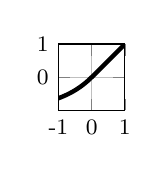
\begin{tikzpicture}
\begin{axis}[
	xmin=-1,xmax=1,
	ymin=-1,ymax=1,
	ytick={0, 1},
	yticklabels={0,1},
	xtick={-1, 0, 1},
	xticklabels={-1,0,1},
	width=.2\textwidth,
	height=.2\textwidth,
	grid=both,
	]
	\addplot [ultra thick,domain=-0.0035:1, samples=10]{x};
	\addplot [ultra thick,domain=-1:0.004, samples=10]{exp(x)-1};
\end{axis}
\end{tikzpicture} &
		%Tanh activation
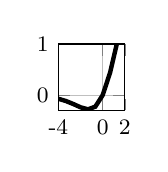
\begin{tikzpicture}
\begin{axis}[
	xmin=-4,xmax=2,
	ymin=-.3,ymax=1,
	ytick={0, 1},
	yticklabels={0,1},
	xtick={-4, 0, 2},
	xticklabels={-4,0,2},
	width=.2\textwidth,
	height=.2\textwidth,
	grid=both,
	]
	\addplot [ultra thick,domain=-4:2, samples=10]{x * (1/ (1+exp(-x)))};
	%\addplot [ultra thick,domain=-1:0.004, samples=10]{exp(x)-1};
\end{axis}
\end{tikzpicture}&
		% This file was created by tikzplotlib v0.9.6.
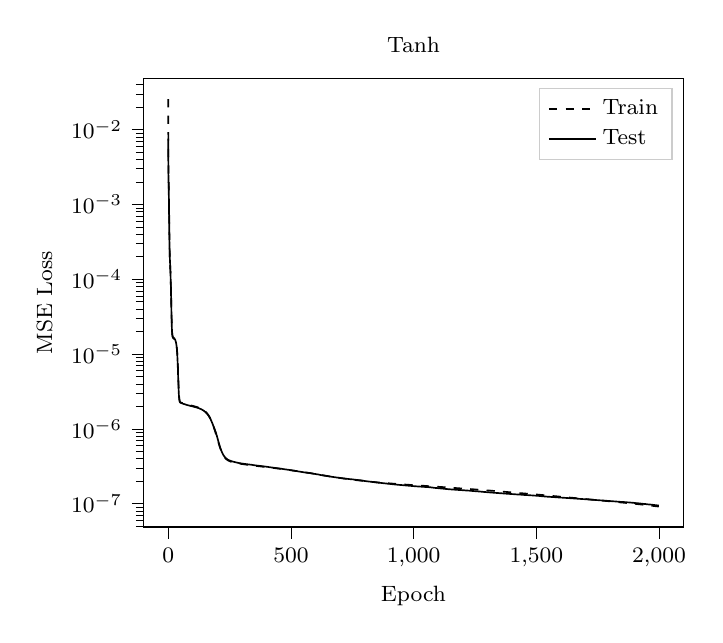
\begin{tikzpicture}

\begin{axis}[
legend cell align={left},
legend style={fill opacity=0.8, draw opacity=1, text opacity=1, draw=white!80!black},
log basis y={10},
tick align=outside,
tick pos=left,
title={Tanh},
x grid style={white!69.0196078431373!black},
xlabel={Epoch},
xmin=-99.95, xmax=2098.95,
xtick style={color=black},
y grid style={white!69.0196078431373!black},
ylabel={MSE Loss},
ymin=4.87162606216586e-08, ymax=0.0480880951021972,
ymode=log,
ytick style={color=black}
]
\addplot [semithick, black, dashed]
table {%
0 0.0256783136818558
1 0.00391949829272926
2 0.00199367450224236
3 0.00143339208001271
4 0.000811647348455153
5 0.000412362531060353
6 0.000244949306972558
7 0.000181991728095454
8 0.000153056107774319
9 0.000130014062575356
10 0.00010614617610554
11 8.2238709928788e-05
12 6.06559043771995e-05
13 4.33234549072949e-05
14 3.11574030747579e-05
15 2.37537921129842e-05
16 1.98036479096118e-05
17 1.79031906054661e-05
18 1.70355609670878e-05
19 1.66247610322898e-05
20 1.63982167177892e-05
21 1.62431279886732e-05
22 1.61158580831398e-05
23 1.59985048476301e-05
24 1.58816735838627e-05
25 1.57583749341939e-05
26 1.56224140046106e-05
27 1.54673897231987e-05
28 1.52862634940902e-05
29 1.50712967133586e-05
30 1.48132416907174e-05
31 1.45002782592201e-05
32 1.41172199300854e-05
33 1.36448685689174e-05
34 1.30603959150903e-05
35 1.23376133224156e-05
36 1.14492682650962e-05
37 1.03756575872467e-05
38 9.12141076651096e-06
39 7.73935586585139e-06
40 6.34618929802855e-06
41 5.09459993941164e-06
42 4.09941510883982e-06
43 3.38837440926909e-06
44 2.91845872209251e-06
45 2.62550942943562e-06
46 2.45301037762147e-06
47 2.35697488326991e-06
48 2.30587279077099e-06
49 2.27869926069957e-06
50 2.26319449416224e-06
51 2.25325485791927e-06
52 2.24564654052983e-06
53 2.23908174814369e-06
54 2.23303946037845e-06
55 2.22724395334239e-06
56 2.22159413002032e-06
57 2.21605597198504e-06
58 2.21059594881012e-06
59 2.20502461627348e-06
60 2.19951089013648e-06
61 2.19409941962567e-06
62 2.18873923640217e-06
63 2.18341688619716e-06
64 2.1780858397733e-06
65 2.1728171752784e-06
66 2.16761157162182e-06
67 2.16247652971902e-06
68 2.15743465199125e-06
69 2.15248080394304e-06
70 2.14761326856205e-06
71 2.14284125951281e-06
72 2.13816882268247e-06
73 2.13358548586484e-06
74 2.12906748606656e-06
75 2.12460380140556e-06
76 2.120198438746e-06
77 2.11584107628937e-06
78 2.11151701626022e-06
79 2.1072322648763e-06
80 2.10301409578051e-06
81 2.09883101015862e-06
82 2.09469965733433e-06
83 2.09061845473002e-06
84 2.08657400560242e-06
85 2.08255163943249e-06
86 2.07854974385668e-06
87 2.07457113936016e-06
88 2.07060074984611e-06
89 2.06666326653249e-06
90 2.06275839008185e-06
91 2.05887886355072e-06
92 2.05505449861221e-06
93 2.0512571416873e-06
94 2.04748774780228e-06
95 2.04372591568358e-06
96 2.03996265599926e-06
97 2.03619106019914e-06
98 2.03241081277383e-06
99 2.02862611661203e-06
100 2.02483424297384e-06
101 2.02102566049689e-06
102 2.01718436369447e-06
103 2.01332004547794e-06
104 2.00943811177012e-06
105 2.00553536137704e-06
106 2.00160756375567e-06
107 1.99764742245634e-06
108 1.99365524949258e-06
109 1.98962802357983e-06
110 1.9855528640278e-06
111 1.98141402830743e-06
112 1.97722682901258e-06
113 1.97299540053564e-06
114 1.96871867424875e-06
115 1.96440277787246e-06
116 1.96000154770104e-06
117 1.9555300951879e-06
118 1.95101178900359e-06
119 1.94641152162944e-06
120 1.94169498476526e-06
121 1.93687540669885e-06
122 1.93201438108304e-06
123 1.92702427668223e-06
124 1.92191399614217e-06
125 1.91670319534865e-06
126 1.91129896376196e-06
127 1.90578242464312e-06
128 1.90011318721872e-06
129 1.89427273897991e-06
130 1.8882123373487e-06
131 1.88198830036868e-06
132 1.87558250883058e-06
133 1.86899712485911e-06
134 1.86227750535295e-06
135 1.85539022578496e-06
136 1.84831423331389e-06
137 1.84095470405055e-06
138 1.83341144793303e-06
139 1.82565649558342e-06
140 1.81764926094274e-06
141 1.8093850391665e-06
142 1.80086963925419e-06
143 1.79206551939615e-06
144 1.78290680096893e-06
145 1.77344423252634e-06
146 1.76363753888609e-06
147 1.75350956513398e-06
148 1.74298757917768e-06
149 1.73214579911019e-06
150 1.72099046380936e-06
151 1.70946602281674e-06
152 1.69748322201713e-06
153 1.68506968657312e-06
154 1.67229672393887e-06
155 1.65912558750847e-06
156 1.64544447042658e-06
157 1.63120314758203e-06
158 1.61646188797704e-06
159 1.60128347954469e-06
160 1.58568593687392e-06
161 1.56952820799461e-06
162 1.55281459512935e-06
163 1.5356757700431e-06
164 1.51809548609094e-06
165 1.50005704529121e-06
166 1.48156487875895e-06
167 1.46263333124352e-06
168 1.44329967625367e-06
169 1.42353404891082e-06
170 1.40324328742736e-06
171 1.38264333622828e-06
172 1.36177704882812e-06
173 1.34056134390903e-06
174 1.31897092293798e-06
175 1.29699397990635e-06
176 1.2747017498782e-06
177 1.25221570530698e-06
178 1.22951809009919e-06
179 1.20664068751353e-06
180 1.18358472803948e-06
181 1.16037225873811e-06
182 1.13706644850708e-06
183 1.11373770050704e-06
184 1.0904470638593e-06
185 1.06723795667563e-06
186 1.04412836427059e-06
187 1.0208118777939e-06
188 9.97641223307255e-07
189 9.74690305525883e-07
190 9.51969390513341e-07
191 9.29392631491055e-07
192 9.06946037218859e-07
193 8.84695177518324e-07
194 8.62814456183969e-07
195 8.41312120513749e-07
196 8.20188414138556e-07
197 7.99479262440173e-07
198 7.79222670900026e-07
199 7.59472292855889e-07
200 7.40254094381498e-07
201 7.21549099239383e-07
202 7.03323363239861e-07
203 6.85619275714089e-07
204 6.6847969463879e-07
205 6.51883700157896e-07
206 6.35866349483649e-07
207 6.20471112625864e-07
208 6.057030220461e-07
209 5.9157178546343e-07
210 5.78070042280387e-07
211 5.65175379023231e-07
212 5.52857127871675e-07
213 5.41098940445295e-07
214 5.29904994237995e-07
215 5.19294521666325e-07
216 5.09250435172248e-07
217 4.99746019073655e-07
218 4.90756391343439e-07
219 4.82253122385146e-07
220 4.74210392084728e-07
221 4.66614737703708e-07
222 4.594722655753e-07
223 4.52780616114978e-07
224 4.46503346267946e-07
225 4.40587696672878e-07
226 4.3501073572827e-07
227 4.29783745403256e-07
228 4.24905776583273e-07
229 4.20343882311158e-07
230 4.16056390292852e-07
231 4.12004934716492e-07
232 4.08168913253348e-07
233 4.04548881093092e-07
234 4.0115957934006e-07
235 3.98017956328545e-07
236 3.95117882121099e-07
237 3.92450205467298e-07
238 3.89984960776246e-07
239 3.87670437433485e-07
240 3.854904206122e-07
241 3.83437721566793e-07
242 3.81521905637783e-07
243 3.79716435688238e-07
244 3.7800730848403e-07
245 3.76387820466562e-07
246 3.74852234386935e-07
247 3.73395006619148e-07
248 3.72012924259479e-07
249 3.70699379175221e-07
250 3.69453458461066e-07
251 3.68269956155132e-07
252 3.67140075951511e-07
253 3.66061015526498e-07
254 3.65028434657688e-07
255 3.64036853241601e-07
256 3.63086354937536e-07
257 3.62170156421371e-07
258 3.61287569361934e-07
259 3.60436046335622e-07
260 3.59612704329493e-07
261 3.58815689537551e-07
262 3.58042329338559e-07
263 3.57291059003728e-07
264 3.56559590528605e-07
265 3.55845987968451e-07
266 3.55149574644997e-07
267 3.54466686573574e-07
268 3.53798637306113e-07
269 3.53151388225115e-07
270 3.52531600483985e-07
271 3.51943575040536e-07
272 3.51372050090504e-07
273 3.50809585640377e-07
274 3.50256817625905e-07
275 3.49712665524748e-07
276 3.49179635776409e-07
277 3.48656109139256e-07
278 3.48143141167157e-07
279 3.47636979228128e-07
280 3.47140434584503e-07
281 3.46653251625639e-07
282 3.46171422521024e-07
283 3.4569364163417e-07
284 3.45216367264811e-07
285 3.44738248372778e-07
286 3.44260469105961e-07
287 3.43785083074977e-07
288 3.43330366902705e-07
289 3.42898308034023e-07
290 3.42464092639716e-07
291 3.42032911291312e-07
292 3.41611756653037e-07
293 3.41200953300813e-07
294 3.4079875696591e-07
295 3.40396311045765e-07
296 3.39994623701045e-07
297 3.39597257266178e-07
298 3.39202901770364e-07
299 3.38812474367955e-07
300 3.38425176110491e-07
301 3.38041470541839e-07
302 3.37660714180288e-07
303 3.37282675587858e-07
304 3.36908611188846e-07
305 3.36536360023842e-07
306 3.36168333262776e-07
307 3.35801948580183e-07
308 3.35437873673072e-07
309 3.350776228217e-07
310 3.34718724388949e-07
311 3.34361913502335e-07
312 3.34007977400574e-07
313 3.3365582474687e-07
314 3.33304566694892e-07
315 3.32955682978309e-07
316 3.32606295486926e-07
317 3.32255786702262e-07
318 3.31905818399036e-07
319 3.31557298508756e-07
320 3.31211877337978e-07
321 3.30875328899083e-07
322 3.30545438856689e-07
323 3.30220234488365e-07
324 3.298965893066e-07
325 3.29574252532439e-07
326 3.29251082263227e-07
327 3.28928731974543e-07
328 3.28607898666178e-07
329 3.28288939684285e-07
330 3.2796907586885e-07
331 3.27652170923898e-07
332 3.27335904060533e-07
333 3.27020988223126e-07
334 3.26706541969202e-07
335 3.26394124385843e-07
336 3.26082249685555e-07
337 3.25770865870823e-07
338 3.25459939233497e-07
339 3.25150717984002e-07
340 3.24840650264946e-07
341 3.24531734875677e-07
342 3.24222071199642e-07
343 3.2391122408626e-07
344 3.23596012492544e-07
345 3.23275019525226e-07
346 3.2294281670886e-07
347 3.22599480000463e-07
348 3.2227435212917e-07
349 3.21953933990926e-07
350 3.21621574045139e-07
351 3.21314297934805e-07
352 3.21034943112863e-07
353 3.20749485581473e-07
354 3.20448250576533e-07
355 3.20144514972753e-07
356 3.19843721285906e-07
357 3.1954650594912e-07
358 3.19254462965546e-07
359 3.18963354061452e-07
360 3.18671405437954e-07
361 3.18381526312805e-07
362 3.1809271050065e-07
363 3.17805669340032e-07
364 3.17520336409416e-07
365 3.17236151289535e-07
366 3.16953998719782e-07
367 3.16672443261723e-07
368 3.16392134422472e-07
369 3.16110889329479e-07
370 3.15829916885946e-07
371 3.15550726682545e-07
372 3.15269492318748e-07
373 3.14990658523584e-07
374 3.14710382866679e-07
375 3.14430895031137e-07
376 3.14152183250371e-07
377 3.13873624463668e-07
378 3.13594867321854e-07
379 3.1331668030532e-07
380 3.13038809508726e-07
381 3.12760674347601e-07
382 3.12483484265158e-07
383 3.12207137426412e-07
384 3.11929519270393e-07
385 3.11651563734472e-07
386 3.11376247253747e-07
387 3.11098750373162e-07
388 3.10823184008768e-07
389 3.10547017605245e-07
390 3.10271550944208e-07
391 3.09995918783557e-07
392 3.09719951715692e-07
393 3.09445476418091e-07
394 3.09168360459466e-07
395 3.08894775159274e-07
396 3.08620413150607e-07
397 3.08344746954958e-07
398 3.08069329236105e-07
399 3.07795802939381e-07
400 3.07521075768591e-07
401 3.07246696138463e-07
402 3.06971505011688e-07
403 3.06696873721535e-07
404 3.06422334631407e-07
405 3.06145008693193e-07
406 3.05865897132662e-07
407 3.05583006166898e-07
408 3.05294879424878e-07
409 3.05009888265317e-07
410 3.04732769805582e-07
411 3.04457269081126e-07
412 3.04181760967026e-07
413 3.03905813524352e-07
414 3.0363094599295e-07
415 3.03357129993742e-07
416 3.03082965743329e-07
417 3.0280785918535e-07
418 3.02532962692226e-07
419 3.0225916734139e-07
420 3.01983990866006e-07
421 3.01708690443547e-07
422 3.01433667928563e-07
423 3.01157673092689e-07
424 3.00882183054796e-07
425 3.00605982133106e-07
426 3.00329158335444e-07
427 3.00052401286166e-07
428 2.99774547642073e-07
429 2.99496324672077e-07
430 2.99217140877772e-07
431 2.98939130772169e-07
432 2.98660514062021e-07
433 2.98383328143359e-07
434 2.98107285431115e-07
435 2.97832286861421e-07
436 2.97559957445515e-07
437 2.97285695779692e-07
438 2.97009015341132e-07
439 2.96733323608578e-07
440 2.96455481390012e-07
441 2.9617858776021e-07
442 2.9590150563763e-07
443 2.95623587916793e-07
444 2.95345244865075e-07
445 2.9506660192169e-07
446 2.94787749211878e-07
447 2.94508583948527e-07
448 2.94228868824575e-07
449 2.93948752528195e-07
450 2.93668269435443e-07
451 2.93385687584191e-07
452 2.93103074923806e-07
453 2.92818450745358e-07
454 2.92533115867855e-07
455 2.92243303405826e-07
456 2.9195033896201e-07
457 2.91650243681829e-07
458 2.91350477510832e-07
459 2.91054979058458e-07
460 2.90767192424823e-07
461 2.90503514534635e-07
462 2.90230797133972e-07
463 2.89949681999246e-07
464 2.89666823135804e-07
465 2.89384619264865e-07
466 2.89102210416559e-07
467 2.88819185129796e-07
468 2.88536360827152e-07
469 2.88253604452393e-07
470 2.87968851523601e-07
471 2.87685964025286e-07
472 2.87401510036034e-07
473 2.87117177379059e-07
474 2.86832849312191e-07
475 2.8654813895912e-07
476 2.86263357793359e-07
477 2.85977837691576e-07
478 2.85691940277388e-07
479 2.85405856359944e-07
480 2.85119550341051e-07
481 2.8483193818829e-07
482 2.84544647684015e-07
483 2.84257998472981e-07
484 2.83969851665233e-07
485 2.83681968156202e-07
486 2.83393235761764e-07
487 2.83104578485904e-07
488 2.82816583634826e-07
489 2.82528103838331e-07
490 2.82238609997876e-07
491 2.81949168339679e-07
492 2.8166003872343e-07
493 2.81370473402376e-07
494 2.81080827463143e-07
495 2.80790753393489e-07
496 2.80500940405659e-07
497 2.80211042010592e-07
498 2.79920554831392e-07
499 2.79629013533622e-07
500 2.79337497119059e-07
501 2.79044599409417e-07
502 2.78752144240002e-07
503 2.78457998902581e-07
504 2.78164109374757e-07
505 2.77869891178284e-07
506 2.77574577594919e-07
507 2.77278857083729e-07
508 2.76983356172877e-07
509 2.7668567361161e-07
510 2.76388693364993e-07
511 2.76090929958173e-07
512 2.75792796927021e-07
513 2.75494566082557e-07
514 2.75195795651939e-07
515 2.74897113726524e-07
516 2.74596931546967e-07
517 2.74297933458456e-07
518 2.7399731402511e-07
519 2.73697588568211e-07
520 2.73398535313163e-07
521 2.73097986720927e-07
522 2.72798081596193e-07
523 2.72497375377156e-07
524 2.721969917161e-07
525 2.71895670650224e-07
526 2.71594623328042e-07
527 2.7129333325604e-07
528 2.70992521649305e-07
529 2.70690323432632e-07
530 2.70388584581838e-07
531 2.70085084920879e-07
532 2.69782810406127e-07
533 2.69479857394117e-07
534 2.69177301504442e-07
535 2.68873798603408e-07
536 2.68569790051743e-07
537 2.68265452916694e-07
538 2.67961485974411e-07
539 2.67657246951103e-07
540 2.67351624302137e-07
541 2.67046286097639e-07
542 2.66741919716651e-07
543 2.66435670084775e-07
544 2.66130026957967e-07
545 2.65824395896175e-07
546 2.6551730083213e-07
547 2.65211784665098e-07
548 2.64905498724488e-07
549 2.64599524172127e-07
550 2.64292502450303e-07
551 2.6398848847009e-07
552 2.63682261532949e-07
553 2.63377035267354e-07
554 2.63071988158003e-07
555 2.62766210369136e-07
556 2.62461571722383e-07
557 2.62156681472447e-07
558 2.61850888776394e-07
559 2.61545947040531e-07
560 2.6124000225991e-07
561 2.60934261390844e-07
562 2.60627847595174e-07
563 2.60322212795927e-07
564 2.60016038239996e-07
565 2.59711214141589e-07
566 2.5940505373967e-07
567 2.59097520512341e-07
568 2.58789286661454e-07
569 2.5847926835354e-07
570 2.5816877410989e-07
571 2.5785619672547e-07
572 2.57544622073169e-07
573 2.57231350587972e-07
574 2.56918664646832e-07
575 2.56602994127775e-07
576 2.56286820288665e-07
577 2.55969035805492e-07
578 2.55648774611927e-07
579 2.5532790500904e-07
580 2.55007268293639e-07
581 2.54691480094493e-07
582 2.54381522779568e-07
583 2.54074222027612e-07
584 2.53768886622652e-07
585 2.53462639946633e-07
586 2.53155078596023e-07
587 2.52848097417768e-07
588 2.52539884442626e-07
589 2.52232671059005e-07
590 2.51926414108539e-07
591 2.51619402433789e-07
592 2.51310856512532e-07
593 2.51001186327926e-07
594 2.50689724069275e-07
595 2.50373325869191e-07
596 2.50046564715944e-07
597 2.4971247898975e-07
598 2.49380338701144e-07
599 2.49063755020984e-07
600 2.48784469974339e-07
601 2.48483565428614e-07
602 2.48175608675183e-07
603 2.47866636698291e-07
604 2.47558843241791e-07
605 2.47249521919457e-07
606 2.4694012356008e-07
607 2.46630496931743e-07
608 2.46319321462352e-07
609 2.4600640222161e-07
610 2.45691713416818e-07
611 2.45375426118244e-07
612 2.45059019846394e-07
613 2.44742416043664e-07
614 2.44427804702241e-07
615 2.44115359791408e-07
616 2.43803189320602e-07
617 2.43488904686728e-07
618 2.43173452574297e-07
619 2.42856562493898e-07
620 2.42540053235984e-07
621 2.4222399055418e-07
622 2.41909370672033e-07
623 2.4159876612373e-07
624 2.41287819818581e-07
625 2.40977986550206e-07
626 2.40667316191434e-07
627 2.40357404365454e-07
628 2.40048627247802e-07
629 2.39740908810404e-07
630 2.39435385040565e-07
631 2.39132102379358e-07
632 2.38831228216441e-07
633 2.38532016894055e-07
634 2.38234100507384e-07
635 2.3793795794802e-07
636 2.37641427077051e-07
637 2.37344928962102e-07
638 2.37049479139273e-07
639 2.36751429071091e-07
640 2.36452641857454e-07
641 2.36152356379193e-07
642 2.35851070470972e-07
643 2.35551766138542e-07
644 2.35254986534983e-07
645 2.34958907981309e-07
646 2.34665752486762e-07
647 2.34375531832143e-07
648 2.34092015489296e-07
649 2.33809699452081e-07
650 2.33527169967829e-07
651 2.33244464084237e-07
652 2.32961468469739e-07
653 2.32677941326642e-07
654 2.32394894752019e-07
655 2.3211163342296e-07
656 2.31829809983708e-07
657 2.31547428853673e-07
658 2.31266236099259e-07
659 2.30985992104138e-07
660 2.30706976715567e-07
661 2.30428674967698e-07
662 2.30152111726056e-07
663 2.29876793980566e-07
664 2.29604099338587e-07
665 2.29333702257861e-07
666 2.29064872783624e-07
667 2.28796595095559e-07
668 2.28530018681283e-07
669 2.2826313580282e-07
670 2.27996663106467e-07
671 2.27733029163346e-07
672 2.27468699684152e-07
673 2.2720402522225e-07
674 2.26941181225016e-07
675 2.26678568793659e-07
676 2.26417082146213e-07
677 2.26155646451787e-07
678 2.25897250800244e-07
679 2.25637136786361e-07
680 2.25378274507193e-07
681 2.25121336775658e-07
682 2.24864484977161e-07
683 2.24608422961126e-07
684 2.24353004966815e-07
685 2.24098303604592e-07
686 2.23845165024272e-07
687 2.23590957716624e-07
688 2.23339868085759e-07
689 2.23087568443248e-07
690 2.22837466004933e-07
691 2.22585833341782e-07
692 2.22337448747112e-07
693 2.22087857792985e-07
694 2.21839565917037e-07
695 2.21591908690755e-07
696 2.21345022012542e-07
697 2.21097984358209e-07
698 2.20852125387694e-07
699 2.2060782892197e-07
700 2.20363927006417e-07
701 2.20120167355731e-07
702 2.19878396393369e-07
703 2.19637687386864e-07
704 2.19396404389727e-07
705 2.19154858328352e-07
706 2.18914575931706e-07
707 2.18667299513697e-07
708 2.18416066260829e-07
709 2.18157695613286e-07
710 2.17917504393483e-07
711 2.17683093978849e-07
712 2.17446162281476e-07
713 2.17212354058915e-07
714 2.16986503602357e-07
715 2.16756925269124e-07
716 2.16528556869378e-07
717 2.16294295185548e-07
718 2.16065943440924e-07
719 2.1583364458877e-07
720 2.15606159549964e-07
721 2.15376262652001e-07
722 2.15151269159719e-07
723 2.14923011839119e-07
724 2.14698939522862e-07
725 2.14466137464342e-07
726 2.14241580749785e-07
727 2.14002345749975e-07
728 2.13779635217293e-07
729 2.13553263428423e-07
730 2.13348029753035e-07
731 2.13115728534774e-07
732 2.12913911404655e-07
733 2.12681533753312e-07
734 2.1250057025668e-07
735 2.12270989564445e-07
736 2.12080155044703e-07
737 2.11840606532121e-07
738 2.11662392217704e-07
739 2.11410442695126e-07
740 2.11244664157562e-07
741 2.10979294507752e-07
742 2.10829887429043e-07
743 2.10549782210023e-07
744 2.10413726215108e-07
745 2.10122939300561e-07
746 2.09999525161209e-07
747 2.09700793199374e-07
748 2.09582869786118e-07
749 2.09277800060192e-07
750 2.09157251006786e-07
751 2.08846759321091e-07
752 2.08716380861063e-07
753 2.08394508241838e-07
754 2.08247044461984e-07
755 2.07928628633169e-07
756 2.07818380481228e-07
757 2.07552191049842e-07
758 2.0744477393464e-07
759 2.07191454308031e-07
760 2.07081657457309e-07
761 2.0683566658164e-07
762 2.06719522203969e-07
763 2.06478433746327e-07
764 2.0635044909767e-07
765 2.06117449401688e-07
766 2.05981543153655e-07
767 2.05756431981285e-07
768 2.0561386548934e-07
769 2.05395930763075e-07
770 2.05249397822627e-07
771 2.05036626113042e-07
772 2.04886012198813e-07
773 2.04679245818795e-07
774 2.04523484633512e-07
775 2.04321535640872e-07
776 2.04161409584458e-07
777 2.03963522885431e-07
778 2.03797197634969e-07
779 2.03599115963016e-07
780 2.03428255403537e-07
781 2.03227953790019e-07
782 2.030431821467e-07
783 2.02847798703942e-07
784 2.02683666543635e-07
785 2.02516986064438e-07
786 2.02353363967234e-07
787 2.02181807019031e-07
788 2.02015970614866e-07
789 2.01841743383113e-07
790 2.01661772905481e-07
791 2.01460166415757e-07
792 2.01229518573598e-07
793 2.01087121354249e-07
794 2.00917898411035e-07
795 2.00780225966923e-07
796 2.00604442376573e-07
797 2.00453189002303e-07
798 2.00287648866038e-07
799 2.00137743007645e-07
800 1.99980189414362e-07
801 1.99827432027178e-07
802 1.99669180005913e-07
803 1.99514663748346e-07
804 1.99357913018616e-07
805 1.99199996849586e-07
806 1.99037115251599e-07
807 1.98870590701006e-07
808 1.98701238232957e-07
809 1.98534945958784e-07
810 1.98443252870106e-07
811 1.98246908794886e-07
812 1.98162096921806e-07
813 1.9793927735634e-07
814 1.97862616772682e-07
815 1.97648748553547e-07
816 1.97567157641743e-07
817 1.97355472479899e-07
818 1.97273760299765e-07
819 1.97065458699797e-07
820 1.96978311969076e-07
821 1.96774255719845e-07
822 1.96680680787154e-07
823 1.96462946391307e-07
824 1.96358382581252e-07
825 1.96272129294073e-07
826 1.96085812284252e-07
827 1.95950416426172e-07
828 1.95843278874008e-07
829 1.95636969095858e-07
830 1.95569540444751e-07
831 1.95350490258761e-07
832 1.95289647095365e-07
833 1.95072461622203e-07
834 1.95013640578168e-07
835 1.94795793944991e-07
836 1.94736558214004e-07
837 1.94521475144427e-07
838 1.94456519217567e-07
839 1.94238834978933e-07
840 1.9416212994372e-07
841 1.93935251495247e-07
842 1.938511577535e-07
843 1.93651539085238e-07
844 1.93595738494423e-07
845 1.93419543499829e-07
846 1.93338983237368e-07
847 1.93155643771092e-07
848 1.93067804922009e-07
849 1.92892168698222e-07
850 1.92794462648749e-07
851 1.92621168871199e-07
852 1.92513661325222e-07
853 1.92361971812716e-07
854 1.92266215115922e-07
855 1.92131815609287e-07
856 1.92028689518509e-07
857 1.91893275420796e-07
858 1.91771540478669e-07
859 1.91640346358213e-07
860 1.91515060819825e-07
861 1.91392229027088e-07
862 1.91263401049468e-07
863 1.91143824686435e-07
864 1.91016867681526e-07
865 1.9089981549314e-07
866 1.90770217429304e-07
867 1.9065634234039e-07
868 1.90525443045431e-07
869 1.90412167242471e-07
870 1.90282269919351e-07
871 1.90172669732647e-07
872 1.90040945632575e-07
873 1.89934002065684e-07
874 1.89798637116212e-07
875 1.89697138701206e-07
876 1.89558307937432e-07
877 1.89464716548571e-07
878 1.89316197278799e-07
879 1.89234877062461e-07
880 1.89073981829324e-07
881 1.89012648903031e-07
882 1.8882984380042e-07
883 1.88791165790292e-07
884 1.88592141974198e-07
885 1.8855339223478e-07
886 1.88359724987208e-07
887 1.88329720955949e-07
888 1.88126539931943e-07
889 1.88094276957429e-07
890 1.87895900772617e-07
891 1.87877068817954e-07
892 1.87662858877502e-07
893 1.87640850128901e-07
894 1.87432238647034e-07
895 1.87432251635755e-07
896 1.87201762059885e-07
897 1.87188818806305e-07
898 1.86971692656357e-07
899 1.86994976040467e-07
900 1.86739167517658e-07
901 1.86732364035436e-07
902 1.86509570291094e-07
903 1.86530011355046e-07
904 1.86241233407713e-07
905 1.86274863906988e-07
906 1.86024884442304e-07
907 1.86029986842584e-07
908 1.85774609136047e-07
909 1.85838526483906e-07
910 1.85592075979457e-07
911 1.85557109972478e-07
912 1.85413238234844e-07
913 1.85311596581528e-07
914 1.85238153171952e-07
915 1.85064903085674e-07
916 1.8492580213092e-07
917 1.84818756245875e-07
918 1.84601177132038e-07
919 1.8463142303915e-07
920 1.84506226155179e-07
921 1.84393604399702e-07
922 1.84358933992712e-07
923 1.84134645067502e-07
924 1.841647220715e-07
925 1.83951926914006e-07
926 1.83905570125376e-07
927 1.83781745690226e-07
928 1.83684701163145e-07
929 1.83511204312481e-07
930 1.8358617639791e-07
931 1.8327896103898e-07
932 1.83298687410627e-07
933 1.83136164785935e-07
934 1.83118544001104e-07
935 1.82905041803849e-07
936 1.82821713821113e-07
937 1.82904439206766e-07
938 1.82656200976794e-07
939 1.82503057061467e-07
940 1.82372852130186e-07
941 1.82464832569451e-07
942 1.82177862498634e-07
943 1.82123570141357e-07
944 1.81958198027132e-07
945 1.82105544006106e-07
946 1.81748656814307e-07
947 1.81644994661667e-07
948 1.81450388794246e-07
949 1.81557134744992e-07
950 1.813367446033e-07
951 1.81250076217054e-07
952 1.8124331060676e-07
953 1.81050296966134e-07
954 1.80912367007124e-07
955 1.81007702494185e-07
956 1.80688111491634e-07
957 1.80711871138328e-07
958 1.80613659338746e-07
959 1.8055098094294e-07
960 1.80342447215764e-07
961 1.80315561223665e-07
962 1.80119200678064e-07
963 1.80223092698384e-07
964 1.79937218476312e-07
965 1.79954523055414e-07
966 1.79713805877668e-07
967 1.79845560126068e-07
968 1.79522391348996e-07
969 1.79567244288137e-07
970 1.794615962325e-07
971 1.79359788418765e-07
972 1.7919894242624e-07
973 1.79157142703446e-07
974 1.78962343092337e-07
975 1.79107667875655e-07
976 1.78761917062786e-07
977 1.78851070963049e-07
978 1.78552461115089e-07
979 1.78618294036426e-07
980 1.78499511285679e-07
981 1.78432811814844e-07
982 1.78235883993239e-07
983 1.7822017412783e-07
984 1.78006425556987e-07
985 1.78184835050388e-07
986 1.77794969182798e-07
987 1.77919801146231e-07
988 1.77607504305399e-07
989 1.77682868525153e-07
990 1.77565874700747e-07
991 1.77483282151059e-07
992 1.77303049056832e-07
993 1.77288027074951e-07
994 1.77071662321282e-07
995 1.77269572674277e-07
996 1.76851885242968e-07
997 1.76987209279389e-07
998 1.76690409439573e-07
999 1.76745455256366e-07
1000 1.76675246279956e-07
1001 1.76517975418733e-07
1002 1.76396269658596e-07
1003 1.76365606833428e-07
1004 1.76154782728588e-07
1005 1.76332453555972e-07
1006 1.75943806638657e-07
1007 1.76068208830316e-07
1008 1.75781630375127e-07
1009 1.75818021048713e-07
1010 1.75775665255173e-07
1011 1.75606383862714e-07
1012 1.75487401570251e-07
1013 1.75443485460391e-07
1014 1.75264921239204e-07
1015 1.75345524404236e-07
1016 1.75081772901819e-07
1017 1.75094191163794e-07
1018 1.75051218050726e-07
1019 1.74866570674226e-07
1020 1.74778132873143e-07
1021 1.74739804535307e-07
1022 1.74538157253323e-07
1023 1.74689216812851e-07
1024 1.74356573701573e-07
1025 1.74413866574241e-07
1026 1.74186691808131e-07
1027 1.74223586959954e-07
1028 1.74151234887177e-07
1029 1.74013387677974e-07
1030 1.7389884820318e-07
1031 1.73856675388606e-07
1032 1.7367983700467e-07
1033 1.73838016891636e-07
1034 1.73464950613322e-07
1035 1.7353948872767e-07
1036 1.733090185283e-07
1037 1.73334884379983e-07
1038 1.73301539497572e-07
1039 1.73104309247663e-07
1040 1.73018324709062e-07
1041 1.72962489585871e-07
1042 1.72787920796225e-07
1043 1.72943589724639e-07
1044 1.72586770247563e-07
1045 1.72631184170768e-07
1046 1.72425827720701e-07
1047 1.72480665220576e-07
1048 1.72308242348151e-07
1049 1.72222635825392e-07
1050 1.72199534759443e-07
1051 1.7209841140442e-07
1052 1.71934404548324e-07
1053 1.71875999363635e-07
1054 1.71818576639282e-07
1055 1.71664782399716e-07
1056 1.71721229904165e-07
1057 1.71507559223016e-07
1058 1.71450052548039e-07
1059 1.71324552624696e-07
1060 1.71405257525237e-07
1061 1.71114308081144e-07
1062 1.71128518353214e-07
1063 1.70986724953082e-07
1064 1.70997916832505e-07
1065 1.70789293711948e-07
1066 1.70840542757844e-07
1067 1.70683409770334e-07
1068 1.70584149131514e-07
1069 1.70473046189556e-07
1070 1.70536510026409e-07
1071 1.70325863329879e-07
1072 1.70239916933212e-07
1073 1.70178448684055e-07
1074 1.70156779681463e-07
1075 1.70017821211843e-07
1076 1.69923560775942e-07
1077 1.69763528241162e-07
1078 1.69926713766699e-07
1079 1.69656568338894e-07
1080 1.6954471659858e-07
1081 1.69526870145376e-07
1082 1.6947657803712e-07
1083 1.69291331680199e-07
1084 1.69387541966159e-07
1085 1.69021876075703e-07
1086 1.69219825430389e-07
1087 1.6888395204262e-07
1088 1.69059036124963e-07
1089 1.68762051210081e-07
1090 1.68699381958959e-07
1091 1.68677553716634e-07
1092 1.6864209008105e-07
1093 1.6840546667396e-07
1094 1.68458437485697e-07
1095 1.68280550276734e-07
1096 1.68226403687299e-07
1097 1.68105190404333e-07
1098 1.68082149194504e-07
1099 1.67917447448929e-07
1100 1.6791531155036e-07
1101 1.67686958455704e-07
1102 1.67809295753329e-07
1103 1.67609576770644e-07
1104 1.67468523144976e-07
1105 1.67500856612435e-07
1106 1.6746117916e-07
1107 1.67153349366345e-07
1108 1.67207376478018e-07
1109 1.67103117760803e-07
1110 1.67111690664967e-07
1111 1.66799030040465e-07
1112 1.66887021485707e-07
1113 1.6675984264225e-07
1114 1.66733511498762e-07
1115 1.66459487857651e-07
1116 1.66677239924695e-07
1117 1.66273404033745e-07
1118 1.66400428263103e-07
1119 1.66187338273005e-07
1120 1.66101584440526e-07
1121 1.66114068328227e-07
1122 1.66078519775681e-07
1123 1.65747365109326e-07
1124 1.65834520352348e-07
1125 1.65732793483642e-07
1126 1.6568083282209e-07
1127 1.65441024208235e-07
1128 1.65423872360293e-07
1129 1.65376426387809e-07
1130 1.65266291709543e-07
1131 1.65075949297488e-07
1132 1.65183653578538e-07
1133 1.64901120811578e-07
1134 1.64889070461527e-07
1135 1.64816789080646e-07
1136 1.64743251978905e-07
1137 1.64549871939812e-07
1138 1.64797036717346e-07
1139 1.64368372125523e-07
1140 1.64327388922914e-07
1141 1.6437572345751e-07
1142 1.64175849306503e-07
1143 1.64098669806378e-07
1144 1.64148435708e-07
1145 1.63833804322167e-07
1146 1.63941523169342e-07
1147 1.6383109585405e-07
1148 1.636207689657e-07
1149 1.6357456372873e-07
1150 1.63597238461932e-07
1151 1.63376890910172e-07
1152 1.63384830955238e-07
1153 1.6318603519494e-07
1154 1.63193474179479e-07
1155 1.6296791127246e-07
1156 1.62943861326426e-07
1157 1.6273880940787e-07
1158 1.62804770901914e-07
1159 1.62569668617607e-07
1160 1.6251618761487e-07
1161 1.62369944625596e-07
1162 1.62474557683368e-07
1163 1.62164271898746e-07
1164 1.62203364439506e-07
1165 1.6202119513764e-07
1166 1.61991749145329e-07
1167 1.61838586954843e-07
1168 1.61991775357251e-07
1169 1.61693534884932e-07
1170 1.61734423144821e-07
1171 1.61486205477956e-07
1172 1.61506580710125e-07
1173 1.61275248807158e-07
1174 1.61340523128217e-07
1175 1.61135238769816e-07
1176 1.6120220598026e-07
1177 1.6093218126656e-07
1178 1.61019107835614e-07
1179 1.60858303864586e-07
1180 1.60795300494954e-07
1181 1.60560779271179e-07
1182 1.606647063781e-07
1183 1.60463883673856e-07
1184 1.60438281078257e-07
1185 1.60245081261223e-07
1186 1.60326889165674e-07
1187 1.60055241750001e-07
1188 1.6013421814165e-07
1189 1.59912973622056e-07
1190 1.59970620472905e-07
1191 1.59738145576682e-07
1192 1.59805658704215e-07
1193 1.5955720218841e-07
1194 1.59621237003194e-07
1195 1.59371404294006e-07
1196 1.59442580354607e-07
1197 1.59209781699587e-07
1198 1.59259970288872e-07
1199 1.59041937585869e-07
1200 1.59072571342733e-07
1201 1.58855913184652e-07
1202 1.58921797947187e-07
1203 1.58672437535756e-07
1204 1.58764354367236e-07
1205 1.58471104839464e-07
1206 1.58557933318093e-07
1207 1.58335334020876e-07
1208 1.58428612778039e-07
1209 1.5810165481156e-07
1210 1.58222141770636e-07
1211 1.57989714331563e-07
1212 1.58009147142479e-07
1213 1.57803747654839e-07
1214 1.57937466838121e-07
1215 1.57602995166428e-07
1216 1.57633344173291e-07
1217 1.57450450885221e-07
1218 1.57564682048417e-07
1219 1.5723370426457e-07
1220 1.57340403383444e-07
1221 1.57073375376626e-07
1222 1.57176691644167e-07
1223 1.5689634754068e-07
1224 1.57032079670216e-07
1225 1.56695187875755e-07
1226 1.56953842733287e-07
1227 1.56568736393581e-07
1228 1.56612420873614e-07
1229 1.56362640737484e-07
1230 1.56375388939978e-07
1231 1.56238784875029e-07
1232 1.56451213698006e-07
1233 1.56064872733452e-07
1234 1.56071111931055e-07
1235 1.55855858885445e-07
1236 1.55867894434891e-07
1237 1.5592698014899e-07
1238 1.55753827151273e-07
1239 1.55547799785438e-07
1240 1.55530699892381e-07
1241 1.55571137803179e-07
1242 1.55404293401773e-07
1243 1.55184656165375e-07
1244 1.55190573323694e-07
1245 1.54982764250633e-07
1246 1.55162933609176e-07
1247 1.54817653481132e-07
1248 1.5485027108042e-07
1249 1.547744172683e-07
1250 1.54679265847335e-07
1251 1.54439792730443e-07
1252 1.54736637590247e-07
1253 1.54300877532876e-07
1254 1.54275749530086e-07
1255 1.54250144028367e-07
1256 1.54043304789298e-07
1257 1.54029483198315e-07
1258 1.53867440310762e-07
1259 1.53782401476121e-07
1260 1.53956117301846e-07
1261 1.53517524005053e-07
1262 1.53721324970491e-07
1263 1.53280332831685e-07
1264 1.53318621009646e-07
1265 1.53157448153252e-07
1266 1.53317707557221e-07
1267 1.53006178400972e-07
1268 1.53078262279394e-07
1269 1.5295192603304e-07
1270 1.52759127885815e-07
1271 1.52895805442199e-07
1272 1.52618819498684e-07
1273 1.52668988391724e-07
1274 1.52435742045043e-07
1275 1.52282082240163e-07
1276 1.52478126885569e-07
1277 1.52267675993301e-07
1278 1.52102081919736e-07
1279 1.51924854762342e-07
1280 1.52071395540077e-07
1281 1.51897150189484e-07
1282 1.5177754506368e-07
1283 1.51588411327452e-07
1284 1.51686713365962e-07
1285 1.51578635318117e-07
1286 1.514046663047e-07
1287 1.51386741720216e-07
1288 1.51236834938118e-07
1289 1.51087039519382e-07
1290 1.51245379640841e-07
1291 1.50855604545086e-07
1292 1.50857793343562e-07
1293 1.50979376975613e-07
1294 1.50700781588853e-07
1295 1.50535089112225e-07
1296 1.50622930220834e-07
1297 1.50551819402267e-07
1298 1.50364579305062e-07
1299 1.50309357970002e-07
1300 1.50167315318583e-07
1301 1.50015147610816e-07
1302 1.50052822462499e-07
1303 1.49995276302661e-07
1304 1.49929092593482e-07
1305 1.49615969156969e-07
1306 1.49589932703975e-07
1307 1.4974333686979e-07
1308 1.49432075829736e-07
1309 1.49371547493615e-07
1310 1.49235247398849e-07
1311 1.49208245971977e-07
1312 1.49100245259604e-07
1313 1.49268570623917e-07
1314 1.48885288751899e-07
1315 1.48768517568953e-07
1316 1.48855611548981e-07
1317 1.4859427885483e-07
1318 1.48693639566488e-07
1319 1.48367197255084e-07
1320 1.48511471429913e-07
1321 1.48261079587542e-07
1322 1.4825105432692e-07
1323 1.48094737163262e-07
1324 1.48087659624707e-07
1325 1.47959285683896e-07
1326 1.47861875170463e-07
1327 1.4779576830648e-07
1328 1.47618505707214e-07
1329 1.47669302762665e-07
1330 1.47545432952256e-07
1331 1.47312891250806e-07
1332 1.47584984269145e-07
1333 1.47121381466775e-07
1334 1.47155481123207e-07
1335 1.47138486575216e-07
1336 1.46936660485153e-07
1337 1.46897626322584e-07
1338 1.46821027406929e-07
1339 1.46725811767112e-07
1340 1.46653712221223e-07
1341 1.46529792196759e-07
1342 1.46487281597274e-07
1343 1.46329400010359e-07
1344 1.46247827714774e-07
1345 1.46147555952325e-07
1346 1.46037953442146e-07
1347 1.45971158666214e-07
1348 1.45886081675428e-07
1349 1.45792722264559e-07
1350 1.45680503919721e-07
1351 1.45593948325029e-07
1352 1.45497979708864e-07
1353 1.45533103278694e-07
1354 1.4527947547549e-07
1355 1.45212114908588e-07
1356 1.45154443664808e-07
1357 1.45234765746238e-07
1358 1.44960471416766e-07
1359 1.44836443077168e-07
1360 1.44837134833153e-07
1361 1.44702509636829e-07
1362 1.44611242220094e-07
1363 1.44524215748731e-07
1364 1.44445664702175e-07
1365 1.44438964461813e-07
1366 1.44254628807516e-07
1367 1.44174589323143e-07
1368 1.44097156415057e-07
1369 1.44165149549735e-07
1370 1.438918012866e-07
1371 1.43834863926884e-07
1372 1.43778407689865e-07
1373 1.43654776103119e-07
1374 1.43601501100932e-07
1375 1.43478440016054e-07
1376 1.43422459309761e-07
1377 1.43299267286068e-07
1378 1.43240890253082e-07
1379 1.43121426198434e-07
1380 1.43058707820387e-07
1381 1.42943359975334e-07
1382 1.42876715720774e-07
1383 1.42766054786136e-07
1384 1.42697908941614e-07
1385 1.42588240770181e-07
1386 1.42517276643161e-07
1387 1.42408500622082e-07
1388 1.42336251322206e-07
1389 1.42228149620394e-07
1390 1.42154443622644e-07
1391 1.42046925965644e-07
1392 1.41968544774329e-07
1393 1.41857630964637e-07
1394 1.41799161355038e-07
1395 1.41669875795003e-07
1396 1.41642744232229e-07
1397 1.41488020773295e-07
1398 1.41444808285485e-07
1399 1.41307266197543e-07
1400 1.41268738268252e-07
1401 1.41131835960095e-07
1402 1.41081490781403e-07
1403 1.4095575309625e-07
1404 1.40900945055478e-07
1405 1.40781008234114e-07
1406 1.40719304582149e-07
1407 1.40605119860027e-07
1408 1.4053854697238e-07
1409 1.40430631219601e-07
1410 1.40360673611895e-07
1411 1.40257951656508e-07
1412 1.40187808121084e-07
1413 1.40090017744399e-07
1414 1.40027148880506e-07
1415 1.39918102711079e-07
1416 1.398644709667e-07
1417 1.39729618609863e-07
1418 1.39709254440845e-07
1419 1.39548208807128e-07
1420 1.39488207395289e-07
1421 1.39385581888973e-07
1422 1.39311794306707e-07
1423 1.39198004013963e-07
1424 1.39159127087396e-07
1425 1.3899639265702e-07
1426 1.38957142148399e-07
1427 1.3883218345967e-07
1428 1.38818436489885e-07
1429 1.38638300825278e-07
1430 1.38555119733041e-07
1431 1.38598182424232e-07
1432 1.38383111163876e-07
1433 1.38299546527776e-07
1434 1.38218821902569e-07
1435 1.38132329730922e-07
1436 1.38036302210764e-07
1437 1.37932765305493e-07
1438 1.37865884262567e-07
1439 1.37768181680542e-07
1440 1.37693862200194e-07
1441 1.37575959314518e-07
1442 1.37563847445676e-07
1443 1.37410551808159e-07
1444 1.37314383366061e-07
1445 1.37217166447101e-07
1446 1.37134599185629e-07
1447 1.37090809047891e-07
1448 1.36948206701959e-07
1449 1.36934800536892e-07
1450 1.36800439307194e-07
1451 1.36791305251904e-07
1452 1.36640489124318e-07
1453 1.36551323684841e-07
1454 1.3647366780134e-07
1455 1.36380717925988e-07
1456 1.36293950461663e-07
1457 1.36197411691796e-07
1458 1.36108559800618e-07
1459 1.36015842777226e-07
1460 1.35925950090154e-07
1461 1.35836153020819e-07
1462 1.35745947254406e-07
1463 1.35656308337673e-07
1464 1.35567192799613e-07
1465 1.35476351189823e-07
1466 1.35388576424589e-07
1467 1.3529987614902e-07
1468 1.35212574981836e-07
1469 1.35123513757662e-07
1470 1.35034041001347e-07
1471 1.34942330241472e-07
1472 1.34852680481856e-07
1473 1.34763203988086e-07
1474 1.34675156090225e-07
1475 1.34583959088275e-07
1476 1.34498445788722e-07
1477 1.34410110952388e-07
1478 1.34325130517254e-07
1479 1.34240905950378e-07
1480 1.34159623293328e-07
1481 1.34082334994901e-07
1482 1.34007962977023e-07
1483 1.3393716164245e-07
1484 1.33868372188317e-07
1485 1.33801153474167e-07
1486 1.33728197575067e-07
1487 1.33651108498611e-07
1488 1.33561932415205e-07
1489 1.33471286439146e-07
1490 1.33377818180236e-07
1491 1.33286574389047e-07
1492 1.33195876379943e-07
1493 1.33103312499827e-07
1494 1.33012573186875e-07
1495 1.32922244659994e-07
1496 1.328316240361e-07
1497 1.32742819303644e-07
1498 1.32652472835559e-07
1499 1.32563086381765e-07
1500 1.32473022716795e-07
1501 1.32383093998101e-07
1502 1.32294703512059e-07
1503 1.32204725133533e-07
1504 1.32114500431157e-07
1505 1.32024823336963e-07
1506 1.31935355909718e-07
1507 1.31843942838827e-07
1508 1.31755951315427e-07
1509 1.31664896130701e-07
1510 1.31577506834901e-07
1511 1.31486739483933e-07
1512 1.31398833772778e-07
1513 1.31310993296552e-07
1514 1.31223457849217e-07
1515 1.31135499088941e-07
1516 1.31049406171257e-07
1517 1.30963723570687e-07
1518 1.30879938801343e-07
1519 1.30797358849577e-07
1520 1.30715271609461e-07
1521 1.30635178784644e-07
1522 1.30553517664111e-07
1523 1.30470073074207e-07
1524 1.30381565455195e-07
1525 1.30291873148281e-07
1526 1.30197957403766e-07
1527 1.30105073552045e-07
1528 1.30015101412084e-07
1529 1.29922131684168e-07
1530 1.29832057609747e-07
1531 1.29743567214291e-07
1532 1.29655932553874e-07
1533 1.29567336209391e-07
1534 1.29478633702718e-07
1535 1.29388707819089e-07
1536 1.29298447703263e-07
1537 1.29211609895208e-07
1538 1.29121361368334e-07
1539 1.2903508240214e-07
1540 1.28947685460901e-07
1541 1.28861089891075e-07
1542 1.28775236419187e-07
1543 1.28692052271617e-07
1544 1.28612261207195e-07
1545 1.2853669561963e-07
1546 1.28464933744965e-07
1547 1.28383591274428e-07
1548 1.28288588584269e-07
1549 1.28192372116587e-07
1550 1.28097349630707e-07
1551 1.28006397964953e-07
1552 1.27916903707614e-07
1553 1.27826293685018e-07
1554 1.27737181870202e-07
1555 1.2764687626543e-07
1556 1.27558287637441e-07
1557 1.2746860927848e-07
1558 1.27379083963319e-07
1559 1.27289022763932e-07
1560 1.272002397954e-07
1561 1.27111350991527e-07
1562 1.27022582084635e-07
1563 1.26932102247679e-07
1564 1.26843040995084e-07
1565 1.26754313335198e-07
1566 1.26665019799077e-07
1567 1.26576261081368e-07
1568 1.26486150506366e-07
1569 1.26398269948425e-07
1570 1.26310102317007e-07
1571 1.26218600009054e-07
1572 1.26132292770365e-07
1573 1.2604147003259e-07
1574 1.2595394938586e-07
1575 1.25864576688173e-07
1576 1.25776658805421e-07
1577 1.25686074447628e-07
1578 1.25598635008828e-07
1579 1.25509957499048e-07
1580 1.25420049670311e-07
1581 1.25333193693677e-07
1582 1.25244157622717e-07
1583 1.25155239857122e-07
1584 1.25067637064546e-07
1585 1.24977565626239e-07
1586 1.24891056422882e-07
1587 1.24802263734125e-07
1588 1.24713928691733e-07
1589 1.24625061047823e-07
1590 1.24537065644859e-07
1591 1.24449508533075e-07
1592 1.24361393055494e-07
1593 1.24273274060727e-07
1594 1.24184724057841e-07
1595 1.24096431704857e-07
1596 1.24009077239862e-07
1597 1.23921701607799e-07
1598 1.23833612477142e-07
1599 1.2374631225498e-07
1600 1.23658226300449e-07
1601 1.2357035235766e-07
1602 1.23482338388214e-07
1603 1.23394856949233e-07
1604 1.23307119714866e-07
1605 1.23220711785166e-07
1606 1.23131181361202e-07
1607 1.23045026157342e-07
1608 1.22957511642596e-07
1609 1.22870412297971e-07
1610 1.22781257239524e-07
1611 1.2269524139441e-07
1612 1.22605206286153e-07
1613 1.2251671019925e-07
1614 1.22426431886424e-07
1615 1.22340115936481e-07
1616 1.22256094321926e-07
1617 1.22175058258733e-07
1618 1.22103615190383e-07
1619 1.2202762109581e-07
1620 1.21916793361265e-07
1621 1.21834089732431e-07
1622 1.21743012215347e-07
1623 1.21660922808076e-07
1624 1.21567334446127e-07
1625 1.21491538585872e-07
1626 1.21390171351266e-07
1627 1.21322823133596e-07
1628 1.21213336576886e-07
1629 1.21154960034175e-07
1630 1.21035876183839e-07
1631 1.20987247662185e-07
1632 1.20860402027745e-07
1633 1.20820134824839e-07
1634 1.2068506220686e-07
1635 1.20652669416188e-07
1636 1.20510663322193e-07
1637 1.20486183746493e-07
1638 1.20336616767247e-07
1639 1.2031963217396e-07
1640 1.20164131615752e-07
1641 1.20150103626315e-07
1642 1.19992589979745e-07
1643 1.19979782780888e-07
1644 1.19823972248412e-07
1645 1.19810623154137e-07
1646 1.19654737659403e-07
1647 1.19639229716029e-07
1648 1.19485491680393e-07
1649 1.19471855569486e-07
1650 1.19316783660395e-07
1651 1.19300847543968e-07
1652 1.19148934437874e-07
1653 1.19132773143349e-07
1654 1.18980588830198e-07
1655 1.18963450141507e-07
1656 1.18812017682046e-07
1657 1.18793472807965e-07
1658 1.18644252474098e-07
1659 1.18625620011414e-07
1660 1.18476356057329e-07
1661 1.18456286585911e-07
1662 1.18310040200242e-07
1663 1.1828933644864e-07
1664 1.18143192537445e-07
1665 1.18121343611222e-07
1666 1.17981712925541e-07
1667 1.1796190426594e-07
1668 1.17837449707281e-07
1669 1.17821046096367e-07
1670 1.17664518249683e-07
1671 1.17625616695705e-07
1672 1.17494159866283e-07
1673 1.17454599340761e-07
1674 1.17330423812234e-07
1675 1.17281875056108e-07
1676 1.17167207086766e-07
1677 1.17112645753537e-07
1678 1.17004529613496e-07
1679 1.16942329213998e-07
1680 1.16840053991041e-07
1681 1.16773833177319e-07
1682 1.16675894744844e-07
1683 1.16606030751143e-07
1684 1.16511720229084e-07
1685 1.16438417961717e-07
1686 1.1634670725158e-07
1687 1.16271883264574e-07
1688 1.16182274517485e-07
1689 1.16104469931599e-07
1690 1.16017207645314e-07
1691 1.15939320814107e-07
1692 1.1585205044895e-07
1693 1.15773689692844e-07
1694 1.15688439173312e-07
1695 1.15609684797846e-07
1696 1.15523752249658e-07
1697 1.15442792669285e-07
1698 1.15360084031124e-07
1699 1.152794114887e-07
1700 1.15195414622349e-07
1701 1.15116151533812e-07
1702 1.15032597470588e-07
1703 1.14952266152102e-07
1704 1.14869341658164e-07
1705 1.14788415693567e-07
1706 1.14706799855924e-07
1707 1.14626587183864e-07
1708 1.14544958570661e-07
1709 1.14467005680297e-07
1710 1.14386371400599e-07
1711 1.14309840782312e-07
1712 1.14231534574571e-07
1713 1.14155406919281e-07
1714 1.14076618189074e-07
1715 1.1400160070707e-07
1716 1.13935357504147e-07
1717 1.13852153852179e-07
1718 1.1374592218516e-07
1719 1.13668901171593e-07
1720 1.13586670188681e-07
1721 1.13503399141734e-07
1722 1.13423729317219e-07
1723 1.13342144530293e-07
1724 1.13260248220115e-07
1725 1.13178309291584e-07
1726 1.13098485158503e-07
1727 1.13015533877103e-07
1728 1.12935625388388e-07
1729 1.12853559258497e-07
1730 1.12772581523757e-07
1731 1.12691697047751e-07
1732 1.12609595291246e-07
1733 1.1252984580068e-07
1734 1.12447377652813e-07
1735 1.12366985916879e-07
1736 1.1228577866973e-07
1737 1.12205130093912e-07
1738 1.12124054268747e-07
1739 1.1204307208601e-07
1740 1.11962179772718e-07
1741 1.11882094351756e-07
1742 1.11800244731342e-07
1743 1.11719630730533e-07
1744 1.11639534196684e-07
1745 1.11557851859345e-07
1746 1.11477907729807e-07
1747 1.11396160754396e-07
1748 1.1131719745805e-07
1749 1.11234583393127e-07
1750 1.11156175847782e-07
1751 1.11073824463404e-07
1752 1.1099390077618e-07
1753 1.10913257636014e-07
1754 1.10833950522249e-07
1755 1.10751658766617e-07
1756 1.10673457989208e-07
1757 1.10590813854117e-07
1758 1.10513686372826e-07
1759 1.10427929719492e-07
1760 1.10354096037213e-07
1761 1.1026718136975e-07
1762 1.10195531284774e-07
1763 1.10103467726219e-07
1764 1.10038613662766e-07
1765 1.09938720179059e-07
1766 1.09883219252538e-07
1767 1.09774770230331e-07
1768 1.09726113770137e-07
1769 1.0961239318874e-07
1770 1.09567085601725e-07
1771 1.09453343561938e-07
1772 1.09406560120817e-07
1773 1.09293789691378e-07
1774 1.09247273940127e-07
1775 1.09132642720056e-07
1776 1.09087160637955e-07
1777 1.08973743436991e-07
1778 1.08927465625186e-07
1779 1.08812749033405e-07
1780 1.08768906656564e-07
1781 1.08653364364386e-07
1782 1.08610696209155e-07
1783 1.08492045278297e-07
1784 1.08451488785022e-07
1785 1.08332703078418e-07
1786 1.08292764849693e-07
1787 1.08172346592994e-07
1788 1.08134267669868e-07
1789 1.08012495928733e-07
1790 1.07974928781118e-07
1791 1.07852817237131e-07
1792 1.07816773052605e-07
1793 1.07694217973631e-07
1794 1.076585755726e-07
1795 1.07533660980152e-07
1796 1.0750032522111e-07
1797 1.07374868321131e-07
1798 1.07341590407373e-07
1799 1.07214731805527e-07
1800 1.07183627001461e-07
1801 1.07055369142017e-07
1802 1.07025273905492e-07
1803 1.06897582774934e-07
1804 1.06866378018822e-07
1805 1.06738425301955e-07
1806 1.06709044885633e-07
1807 1.06578284807313e-07
1808 1.06551349951189e-07
1809 1.06419266913349e-07
1810 1.06393436325902e-07
1811 1.0626070748998e-07
1812 1.06233781600906e-07
1813 1.06102325410973e-07
1814 1.06077179772512e-07
1815 1.05943803617947e-07
1816 1.05918884933942e-07
1817 1.05785039274053e-07
1818 1.0576097081838e-07
1819 1.05625972793177e-07
1820 1.05602148408934e-07
1821 1.05468074529824e-07
1822 1.05444441423685e-07
1823 1.05309890450656e-07
1824 1.05286905679236e-07
1825 1.05151352997268e-07
1826 1.05128677049038e-07
1827 1.04993245805929e-07
1828 1.04970954780015e-07
1829 1.04834349158978e-07
1830 1.04813155957117e-07
1831 1.04675824211142e-07
1832 1.04656024795702e-07
1833 1.04517476188448e-07
1834 1.04497554922034e-07
1835 1.04359976702995e-07
1836 1.04338933539339e-07
1837 1.04202867277081e-07
1838 1.04181184603647e-07
1839 1.04044154433325e-07
1840 1.04023431063638e-07
1841 1.03886127348574e-07
1842 1.03865805684222e-07
1843 1.03730083061748e-07
1844 1.03708399777247e-07
1845 1.03575531461786e-07
1846 1.03553730738781e-07
1847 1.03431781575125e-07
1848 1.03406835641806e-07
1849 1.03251629880674e-07
1850 1.03248295282299e-07
1851 1.03094720223851e-07
1852 1.03084822235644e-07
1853 1.029415868814e-07
1854 1.02924780257752e-07
1855 1.02787245204183e-07
1856 1.02766203596616e-07
1857 1.02631769628658e-07
1858 1.02608433905971e-07
1859 1.02473619911336e-07
1860 1.02450679698052e-07
1861 1.02315491744775e-07
1862 1.02293353030802e-07
1863 1.02158083478798e-07
1864 1.02137613730235e-07
1865 1.02001180536604e-07
1866 1.01981320298705e-07
1867 1.0184516611389e-07
1868 1.0182440312434e-07
1869 1.01688210200734e-07
1870 1.01670011382282e-07
1871 1.01530907663516e-07
1872 1.01513423203414e-07
1873 1.01376702275502e-07
1874 1.01358417559538e-07
1875 1.01222969291825e-07
1876 1.01205789569292e-07
1877 1.01067017183709e-07
1878 1.01052819672987e-07
1879 1.00915272618352e-07
1880 1.0090144083108e-07
1881 1.00764368340833e-07
1882 1.00751233624408e-07
1883 1.00615954877981e-07
1884 1.00604420119055e-07
1885 1.0046848284162e-07
1886 1.00461983791433e-07
1887 1.00328959490525e-07
1888 1.00327407132283e-07
1889 1.00198732020829e-07
1890 1.00210742438378e-07
1891 1.00091209333186e-07
1892 1.00120992215125e-07
1893 1.00010873573808e-07
1894 1.00031446216065e-07
1895 9.98494305122222e-08
1896 9.98177236226638e-08
1897 9.96636280206076e-08
1898 9.9662101789022e-08
1899 9.95036318087727e-08
1900 9.95035710644743e-08
1901 9.93359447178932e-08
1902 9.93463889713553e-08
1903 9.91639390761634e-08
1904 9.91915004178168e-08
1905 9.89930967563168e-08
1906 9.90359007531083e-08
1907 9.88282890048708e-08
1908 9.88751828856493e-08
1909 9.86779837575114e-08
1910 9.86860634668574e-08
1911 9.85199047107699e-08
1912 9.85522943679484e-08
1913 9.83903354097038e-08
1914 9.83319166465435e-08
1915 9.82184653537388e-08
1916 9.81738594347803e-08
1917 9.80355162667479e-08
1918 9.80704097628404e-08
1919 9.79550177007127e-08
1920 9.79253364477017e-08
1921 9.7782193442697e-08
1922 9.76768999620958e-08
1923 9.76173793958424e-08
1924 9.75287996425322e-08
1925 9.74686554826576e-08
1926 9.73918850419864e-08
1927 9.72836267649768e-08
1928 9.73122499345891e-08
1929 9.7137337192521e-08
1930 9.70798927966143e-08
1931 9.69518271602965e-08
1932 9.69189093709133e-08
1933 9.67950209869173e-08
1934 9.67396970565915e-08
1935 9.66325465867612e-08
1936 9.65764778655398e-08
1937 9.64863556447426e-08
1938 9.63525852242242e-08
1939 9.63383329022349e-08
1940 9.61832626558135e-08
1941 9.61392340954603e-08
1942 9.59978614645252e-08
1943 9.59531415389847e-08
1944 9.57992250434359e-08
1945 9.57176675484561e-08
1946 9.56372701708119e-08
1947 9.55616131150805e-08
1948 9.55027764604211e-08
1949 9.54192266604537e-08
1950 9.52890652783367e-08
1951 9.52766380919456e-08
1952 9.51284585539724e-08
1953 9.50952942702088e-08
1954 9.4968490913061e-08
1955 9.49355355217563e-08
1956 9.48217696077336e-08
1957 9.47154426356178e-08
1958 9.46745343597399e-08
1959 9.45576307387341e-08
1960 9.44733649959062e-08
1961 9.44023931381821e-08
1962 9.43122054337664e-08
1963 9.42393481651038e-08
1964 9.41573721391364e-08
1965 9.40662891650845e-08
1966 9.40114193213049e-08
1967 9.39233958447971e-08
1968 9.38029722874489e-08
1969 9.37450194555822e-08
1970 9.36574502858889e-08
1971 9.35782248561168e-08
1972 9.34887714336696e-08
1973 9.3408080211077e-08
1974 9.33098989790437e-08
1975 9.32318668986909e-08
1976 9.31109529389573e-08
1977 9.30678109511973e-08
1978 9.29844462476126e-08
1979 9.28701786762076e-08
1980 9.28146823682141e-08
1981 9.27165723680901e-08
1982 9.26600080148887e-08
1983 9.25481256501825e-08
1984 9.24809953559702e-08
1985 9.238034407133e-08
1986 9.2328959901522e-08
1987 9.22276714661052e-08
1988 9.21186526383622e-08
1989 9.20790567349172e-08
1990 9.19701495902814e-08
1991 9.18760605159719e-08
1992 9.18214794936034e-08
1993 9.17084328833084e-08
1994 9.16553286174349e-08
1995 9.15473841729408e-08
1996 9.14629573642856e-08
1997 9.13915596143511e-08
1998 9.12936959593935e-08
1999 9.12315428038823e-08
};
\addlegendentry{Train}
\addplot [semithick, black]
table {%
0 0.00757189933210611
1 0.00231354776769876
2 0.00172689720056951
3 0.00111725344322622
4 0.000576228136196733
5 0.000321307015838102
6 0.000222852322622202
7 0.00018314401677344
8 0.000157202070113271
9 0.000131142092868686
10 0.000103817488707136
11 7.77645473135635e-05
12 5.55872247787192e-05
13 3.89783745049499e-05
14 2.82207911368459e-05
15 2.21843656618148e-05
16 1.91927338164533e-05
17 1.78358131961431e-05
18 1.72350355569506e-05
19 1.69452778209234e-05
20 1.67743528436404e-05
21 1.66473146236967e-05
22 1.65352812473429e-05
23 1.64228040375747e-05
24 1.6300236893585e-05
25 1.61624484462664e-05
26 1.60050221893471e-05
27 1.58211023517651e-05
28 1.56023888848722e-05
29 1.53401488205418e-05
30 1.50225159813999e-05
31 1.46344837048673e-05
32 1.41610498758382e-05
33 1.35855179905775e-05
34 1.28874389702105e-05
35 1.20397271530237e-05
36 1.10160563053796e-05
37 9.80650656856596e-06
38 8.43856741994387e-06
39 6.99934525982826e-06
40 5.63651110496721e-06
41 4.49852859674138e-06
42 3.65314713235421e-06
43 3.07963659906818e-06
44 2.71202293333772e-06
45 2.48932860813511e-06
46 2.36340451920114e-06
47 2.29604233936698e-06
48 2.26174938688928e-06
49 2.24436098505976e-06
50 2.23402162191633e-06
51 2.22632638724463e-06
52 2.21947198042471e-06
53 2.21231721297954e-06
54 2.20599281419709e-06
55 2.20017341234779e-06
56 2.19425942304952e-06
57 2.18812738239649e-06
58 2.18169157051307e-06
59 2.17522529055714e-06
60 2.16870125768764e-06
61 2.16252578866261e-06
62 2.15704108086356e-06
63 2.15156410376949e-06
64 2.14648275687068e-06
65 2.14147098631656e-06
66 2.13616635846847e-06
67 2.13079192690202e-06
68 2.12541522159881e-06
69 2.1200858100201e-06
70 2.11486621992663e-06
71 2.10983034776291e-06
72 2.1049518181826e-06
73 2.10016810342495e-06
74 2.09545669349609e-06
75 2.09080417334917e-06
76 2.08621918318386e-06
77 2.08170968107879e-06
78 2.07733137358446e-06
79 2.07305447474937e-06
80 2.06868594432308e-06
81 2.06437994165753e-06
82 2.06043318939919e-06
83 2.05644232664781e-06
84 2.0524073534034e-06
85 2.04834668693366e-06
86 2.04438651962846e-06
87 2.04050184038351e-06
88 2.03653394237335e-06
89 2.03256013264763e-06
90 2.02859519049525e-06
91 2.02469618670875e-06
92 2.02088699552405e-06
93 2.01716375158867e-06
94 2.01350235329301e-06
95 2.00988574761141e-06
96 2.00627096091921e-06
97 2.00259637495037e-06
98 1.99885994334181e-06
99 1.99508667719783e-06
100 1.99131750378001e-06
101 1.98756606550887e-06
102 1.98379348148592e-06
103 1.97998292605917e-06
104 1.97613053387613e-06
105 1.97224085241032e-06
106 1.96831024368294e-06
107 1.96435007637774e-06
108 1.96036580746295e-06
109 1.95635175259667e-06
110 1.95229063137958e-06
111 1.94816198018088e-06
112 1.94399422071001e-06
113 1.93980258700321e-06
114 1.9355888980499e-06
115 1.93136861526e-06
116 1.92722677638812e-06
117 1.92289826372871e-06
118 1.91830258700065e-06
119 1.91340882338409e-06
120 1.90855348591867e-06
121 1.90414561984653e-06
122 1.89889465218585e-06
123 1.89397746908071e-06
124 1.88939679901523e-06
125 1.88414048807317e-06
126 1.87855380318069e-06
127 1.87314526556293e-06
128 1.86755323738907e-06
129 1.86166766980023e-06
130 1.85547753517312e-06
131 1.84901341526711e-06
132 1.84264706604154e-06
133 1.83605436632206e-06
134 1.82956421213021e-06
135 1.82338919785252e-06
136 1.81552900357929e-06
137 1.80827692020102e-06
138 1.80085896772653e-06
139 1.79312894488248e-06
140 1.78544337359199e-06
141 1.77783579147217e-06
142 1.76977698629344e-06
143 1.76120738615282e-06
144 1.75235982169397e-06
145 1.74406659425586e-06
146 1.73541684489464e-06
147 1.72538182141579e-06
148 1.71526744452422e-06
149 1.70504654306569e-06
150 1.69440045283409e-06
151 1.68317467341694e-06
152 1.67212203905365e-06
153 1.66097026976786e-06
154 1.64922550993651e-06
155 1.6366448107874e-06
156 1.62349863330746e-06
157 1.61000264142785e-06
158 1.59640455876797e-06
159 1.5825156651772e-06
160 1.56760324898642e-06
161 1.55271811763669e-06
162 1.53781195422198e-06
163 1.5225629113047e-06
164 1.50687731093058e-06
165 1.49068762311799e-06
166 1.47391403970687e-06
167 1.456628865526e-06
168 1.43905299410108e-06
169 1.41962095767667e-06
170 1.39984229008405e-06
171 1.37973813707504e-06
172 1.35911807319644e-06
173 1.33792514134257e-06
174 1.31609863274207e-06
175 1.29385193758935e-06
176 1.27185285236919e-06
177 1.24993607641954e-06
178 1.22776793887169e-06
179 1.20523759505886e-06
180 1.18257298709068e-06
181 1.16014371087658e-06
182 1.1381328022253e-06
183 1.11657402612764e-06
184 1.09565598904737e-06
185 1.07576920527208e-06
186 1.05480546608305e-06
187 1.03400623174821e-06
188 1.01384318895725e-06
189 9.94196057035879e-07
190 9.75076432041533e-07
191 9.54211259340809e-07
192 9.33810667902435e-07
193 9.13567589577724e-07
194 8.93540118340752e-07
195 8.7334251475113e-07
196 8.52891048452875e-07
197 8.32212890600204e-07
198 8.11159679869888e-07
199 7.90065314504318e-07
200 7.69062353356276e-07
201 7.48205820855219e-07
202 7.27842859760131e-07
203 7.08114953340555e-07
204 6.88830937178864e-07
205 6.70056067519909e-07
206 6.51937568818539e-07
207 6.344951657411e-07
208 6.17837599747872e-07
209 6.02160469043156e-07
210 5.87514819017088e-07
211 5.7384960427953e-07
212 5.60921989745111e-07
213 5.48473678918526e-07
214 5.36510526671918e-07
215 5.25344830748509e-07
216 5.15033946157928e-07
217 5.05386367422034e-07
218 4.96285395001905e-07
219 4.87689192141261e-07
220 4.79516529594548e-07
221 4.71730061235576e-07
222 4.64458850046867e-07
223 4.57714065760229e-07
224 4.51481156460432e-07
225 4.45709758878365e-07
226 4.40336776819095e-07
227 4.35368264106728e-07
228 4.30750020541382e-07
229 4.26469654257744e-07
230 4.22478933614912e-07
231 4.18747390540375e-07
232 4.15171484746679e-07
233 4.11659840438006e-07
234 4.08245057315071e-07
235 4.04999781267179e-07
236 4.02141182576088e-07
237 3.99803269601762e-07
238 3.97628497239566e-07
239 3.95445340473088e-07
240 3.93182233437983e-07
241 3.91090793527837e-07
242 3.89197737149516e-07
243 3.87470691975977e-07
244 3.85885044806855e-07
245 3.84415926646398e-07
246 3.83027412453885e-07
247 3.81678120220386e-07
248 3.80339741923308e-07
249 3.78988659122115e-07
250 3.77662075834451e-07
251 3.76379944100336e-07
252 3.75157839016538e-07
253 3.73988797264246e-07
254 3.72877764220902e-07
255 3.71828406287023e-07
256 3.70837085483799e-07
257 3.69894536333959e-07
258 3.68992459698347e-07
259 3.6814256532125e-07
260 3.67322599004183e-07
261 3.66545179986133e-07
262 3.65790839396141e-07
263 3.65060742524292e-07
264 3.64350427162208e-07
265 3.63658926971766e-07
266 3.6297012684372e-07
267 3.62264984232752e-07
268 3.61526559800041e-07
269 3.60765056939272e-07
270 3.60008925781585e-07
271 3.59255551529714e-07
272 3.58531451638555e-07
273 3.57854787580436e-07
274 3.57219846591761e-07
275 3.56612247287558e-07
276 3.56021757852432e-07
277 3.55441471810991e-07
278 3.54872724983579e-07
279 3.5430537081993e-07
280 3.53727727997466e-07
281 3.53136783814989e-07
282 3.52505253431445e-07
283 3.51853060465146e-07
284 3.51204761273038e-07
285 3.50592699760455e-07
286 3.50021139183809e-07
287 3.49473793903599e-07
288 3.48943643757593e-07
289 3.48437907859989e-07
290 3.47962895830278e-07
291 3.47516419196836e-07
292 3.47084636587169e-07
293 3.46643815873904e-07
294 3.46207571055857e-07
295 3.45778602195423e-07
296 3.45349405961315e-07
297 3.44927741480205e-07
298 3.44512613992265e-07
299 3.44105728800059e-07
300 3.43703817407004e-07
301 3.43302190231043e-07
302 3.42907014783123e-07
303 3.42518376328371e-07
304 3.42130419994646e-07
305 3.41749966992211e-07
306 3.4137428883696e-07
307 3.40999292802735e-07
308 3.40631828521509e-07
309 3.40271498089351e-07
310 3.39915942504376e-07
311 3.39561637474617e-07
312 3.3922066222658e-07
313 3.38877697458884e-07
314 3.38540672828458e-07
315 3.38199868110678e-07
316 3.37851616905027e-07
317 3.37482163104141e-07
318 3.37094775204605e-07
319 3.36706733605752e-07
320 3.36351888563513e-07
321 3.36034361225757e-07
322 3.35738150170073e-07
323 3.35447850829951e-07
324 3.35154368258372e-07
325 3.34855684513968e-07
326 3.34556517600504e-07
327 3.34259254941571e-07
328 3.33956762688103e-07
329 3.33655520989851e-07
330 3.33354051917922e-07
331 3.33054515522235e-07
332 3.32753842258171e-07
333 3.32451463691541e-07
334 3.3215061989722e-07
335 3.31850685597601e-07
336 3.31551120780205e-07
337 3.31250816998363e-07
338 3.30956197558407e-07
339 3.30654899016736e-07
340 3.30352634136943e-07
341 3.30052529307068e-07
342 3.29739606286239e-07
343 3.29404372223507e-07
344 3.29015591660209e-07
345 3.28506928326533e-07
346 3.27803860500353e-07
347 3.27093715668525e-07
348 3.26682112472554e-07
349 3.26361146107956e-07
350 3.26064309774665e-07
351 3.25769036635393e-07
352 3.25465521200385e-07
353 3.2514194003852e-07
354 3.24804005913393e-07
355 3.2445936426484e-07
356 3.2412404493698e-07
357 3.2380171433033e-07
358 3.23506583299604e-07
359 3.23233706467363e-07
360 3.2297887742061e-07
361 3.2273538863592e-07
362 3.22502614835685e-07
363 3.22266515695446e-07
364 3.2202081001742e-07
365 3.21777207545892e-07
366 3.21515415180329e-07
367 3.21252258572713e-07
368 3.20981712320645e-07
369 3.20703321676774e-07
370 3.20423680477688e-07
371 3.20136365417056e-07
372 3.19852574648394e-07
373 3.19564719575283e-07
374 3.19271521220799e-07
375 3.1898002816888e-07
376 3.1868364658294e-07
377 3.18386923936487e-07
378 3.18089206530203e-07
379 3.17792569148878e-07
380 3.1749257800584e-07
381 3.17192132115451e-07
382 3.16892339924379e-07
383 3.16590472948519e-07
384 3.16285337476074e-07
385 3.15979974629954e-07
386 3.15677851858709e-07
387 3.15374336423702e-07
388 3.15068149348008e-07
389 3.14764093900521e-07
390 3.14461033212865e-07
391 3.14160985226408e-07
392 3.13857782430205e-07
393 3.13559326059476e-07
394 3.13264166607041e-07
395 3.12967046056656e-07
396 3.126754393179e-07
397 3.12380734612816e-07
398 3.12092197418679e-07
399 3.1180573500933e-07
400 3.11520835793999e-07
401 3.1123687449508e-07
402 3.109554427283e-07
403 3.10673982539811e-07
404 3.10383768464817e-07
405 3.10078576148953e-07
406 3.09742489434939e-07
407 3.09323354485969e-07
408 3.08814122718104e-07
409 3.08301679297074e-07
410 3.07875410499037e-07
411 3.07510362063113e-07
412 3.07177742797649e-07
413 3.06860954424337e-07
414 3.06547633499576e-07
415 3.06238348457555e-07
416 3.05929802379978e-07
417 3.05623501617447e-07
418 3.05316746107565e-07
419 3.0501209380418e-07
420 3.04705650933101e-07
421 3.04400629147494e-07
422 3.04095436831631e-07
423 3.03792347722265e-07
424 3.0348772384059e-07
425 3.03186652672593e-07
426 3.02881346669892e-07
427 3.0258306082942e-07
428 3.02280739106209e-07
429 3.01978758443511e-07
430 3.01679307312952e-07
431 3.01367464317082e-07
432 3.01058463492154e-07
433 3.00743096204314e-07
434 3.00439211287085e-07
435 3.00134502140281e-07
436 2.99837438433315e-07
437 2.99543046367035e-07
438 2.99252008062467e-07
439 2.98959179190206e-07
440 2.98670812526325e-07
441 2.98377415219875e-07
442 2.98092288630869e-07
443 2.97805769378101e-07
444 2.97516294267552e-07
445 2.97226904422132e-07
446 2.96939759891757e-07
447 2.96649517395053e-07
448 2.96361463369976e-07
449 2.9607238616336e-07
450 2.95783678438966e-07
451 2.9549653390859e-07
452 2.95206461942144e-07
453 2.94913974130395e-07
454 2.94622765295571e-07
455 2.94328202699035e-07
456 2.94032219017026e-07
457 2.93726856170906e-07
458 2.93400375994679e-07
459 2.93056245936896e-07
460 2.92704640969532e-07
461 2.92339279894804e-07
462 2.91982189537521e-07
463 2.916349330917e-07
464 2.91295805254776e-07
465 2.90963839688629e-07
466 2.90640571165568e-07
467 2.9031514259259e-07
468 2.89994574131924e-07
469 2.89677274167843e-07
470 2.8935261298102e-07
471 2.89030936073686e-07
472 2.88709486540029e-07
473 2.88387298041926e-07
474 2.88059794684159e-07
475 2.87732376591521e-07
476 2.87408454369142e-07
477 2.87082883687617e-07
478 2.86762286805242e-07
479 2.86445697383897e-07
480 2.86128852167167e-07
481 2.85815588085825e-07
482 2.85504285102434e-07
483 2.8518959993562e-07
484 2.84878638012742e-07
485 2.84563554941997e-07
486 2.84243895976033e-07
487 2.83925572830412e-07
488 2.8360332748889e-07
489 2.83278296819844e-07
490 2.82954090380372e-07
491 2.82632413473038e-07
492 2.82310963939381e-07
493 2.81987439620934e-07
494 2.81669628066084e-07
495 2.8134996910012e-07
496 2.81029997495352e-07
497 2.8070328994545e-07
498 2.80369363281352e-07
499 2.8002617113998e-07
500 2.79674736702873e-07
501 2.79321369589525e-07
502 2.78964876088139e-07
503 2.78612588999749e-07
504 2.78259335573239e-07
505 2.77912278079384e-07
506 2.77564993211854e-07
507 2.77221516853388e-07
508 2.76879177363298e-07
509 2.76540163213213e-07
510 2.76203877547232e-07
511 2.75865488674754e-07
512 2.75532954674418e-07
513 2.75196896382113e-07
514 2.74859843329978e-07
515 2.74528446198019e-07
516 2.74192359484005e-07
517 2.73856898047597e-07
518 2.73519759730334e-07
519 2.73187993116153e-07
520 2.72854521199406e-07
521 2.72520907174112e-07
522 2.72190249006599e-07
523 2.71860500333787e-07
524 2.71530780082685e-07
525 2.71202821977568e-07
526 2.70876626018435e-07
527 2.70549492142891e-07
528 2.70224234100169e-07
529 2.69898720262063e-07
530 2.69571984290451e-07
531 2.69245134632001e-07
532 2.68921638735264e-07
533 2.68594334329464e-07
534 2.68267854153237e-07
535 2.67942539267096e-07
536 2.67619753913095e-07
537 2.67293870592766e-07
538 2.66968754658592e-07
539 2.66641421831082e-07
540 2.66317840669217e-07
541 2.65991502601537e-07
542 2.65664453991121e-07
543 2.65339707539169e-07
544 2.65014250544482e-07
545 2.64691379925353e-07
546 2.64365638713571e-07
547 2.64044984987777e-07
548 2.63720068005568e-07
549 2.63397822664047e-07
550 2.63078590023724e-07
551 2.62759584757077e-07
552 2.6244461537317e-07
553 2.62132488160205e-07
554 2.61824112612885e-07
555 2.61524007783009e-07
556 2.61230638898269e-07
557 2.60943522789603e-07
558 2.60669281715309e-07
559 2.6040129341709e-07
560 2.60138591556824e-07
561 2.59882455111438e-07
562 2.59628933463318e-07
563 2.59385018352987e-07
564 2.59151164527793e-07
565 2.58942520758865e-07
566 2.58750475268243e-07
567 2.58566956290451e-07
568 2.58378776152313e-07
569 2.58176783063391e-07
570 2.57968707728651e-07
571 2.57760461863654e-07
572 2.57557303484646e-07
573 2.57359033639659e-07
574 2.57157324767832e-07
575 2.56948908372578e-07
576 2.5672730430415e-07
577 2.56481172300482e-07
578 2.56194681469424e-07
579 2.55848647157109e-07
580 2.55444007279948e-07
581 2.55011542549255e-07
582 2.54571631330691e-07
583 2.54148005751631e-07
584 2.53743763778402e-07
585 2.53355608492711e-07
586 2.52980498771649e-07
587 2.52618235663249e-07
588 2.52268222311613e-07
589 2.51927446015543e-07
590 2.51595594136234e-07
591 2.51268488682399e-07
592 2.5095059186242e-07
593 2.50635537213384e-07
594 2.50326053219396e-07
595 2.50023333592253e-07
596 2.49735393254014e-07
597 2.49446429734235e-07
598 2.49116368422619e-07
599 2.4881194349291e-07
600 2.48514169243208e-07
601 2.48223216203769e-07
602 2.47939027531174e-07
603 2.47653616725074e-07
604 2.47365477434869e-07
605 2.47078219217656e-07
606 2.4678212184881e-07
607 2.46486820287828e-07
608 2.4618032057333e-07
609 2.45870921844471e-07
610 2.45555440869794e-07
611 2.45229017536985e-07
612 2.44890344447413e-07
613 2.44539990035264e-07
614 2.44178238517634e-07
615 2.43809381572646e-07
616 2.43427706436705e-07
617 2.43029631974423e-07
618 2.42622860469055e-07
619 2.42207619294277e-07
620 2.41795447664117e-07
621 2.41404535472611e-07
622 2.41036303805231e-07
623 2.40693424302663e-07
624 2.40371036852594e-07
625 2.40052685285264e-07
626 2.39740927554521e-07
627 2.39421268588558e-07
628 2.39106356048069e-07
629 2.38784906514411e-07
630 2.38469425539733e-07
631 2.38150050790864e-07
632 2.37837852523626e-07
633 2.37528468005621e-07
634 2.37222010923688e-07
635 2.36925814078859e-07
636 2.36628210359413e-07
637 2.36337982073564e-07
638 2.36051988622421e-07
639 2.35765782008457e-07
640 2.35482957577915e-07
641 2.35203231113701e-07
642 2.34919184549653e-07
643 2.34646961416729e-07
644 2.34390839182197e-07
645 2.34140870247757e-07
646 2.33870935062441e-07
647 2.33569480201368e-07
648 2.3325499398652e-07
649 2.32940266187143e-07
650 2.32636210739656e-07
651 2.32337924899184e-07
652 2.320469860706e-07
653 2.31758917834668e-07
654 2.31476832368571e-07
655 2.31193894251192e-07
656 2.30918104193734e-07
657 2.30646762133802e-07
658 2.30380379662165e-07
659 2.30118217814379e-07
660 2.29871318424557e-07
661 2.2962768753132e-07
662 2.29394686357409e-07
663 2.29170822763081e-07
664 2.28947499181231e-07
665 2.28722598194508e-07
666 2.28496290333169e-07
667 2.28261441748145e-07
668 2.28024831017137e-07
669 2.27784923367835e-07
670 2.27541050890068e-07
671 2.27295089416657e-07
672 2.27049966383674e-07
673 2.26804843350692e-07
674 2.26557162363861e-07
675 2.2631367357917e-07
676 2.26065239417039e-07
677 2.25820556920553e-07
678 2.25574339651757e-07
679 2.25329259251339e-07
680 2.25084136218356e-07
681 2.24843759610849e-07
682 2.24597656028891e-07
683 2.24354977262919e-07
684 2.24112014279854e-07
685 2.23870017634908e-07
686 2.23628575213297e-07
687 2.23390529185963e-07
688 2.23148475697599e-07
689 2.22911822334027e-07
690 2.22674387373445e-07
691 2.22437762431582e-07
692 2.2220611128887e-07
693 2.21973422753763e-07
694 2.21740450001562e-07
695 2.21511655240647e-07
696 2.21281027279474e-07
697 2.21056495774974e-07
698 2.20832745867483e-07
699 2.20610672840849e-07
700 2.20383839177885e-07
701 2.20157573949109e-07
702 2.19931777678539e-07
703 2.19701050241383e-07
704 2.19468347495422e-07
705 2.19231381493046e-07
706 2.1897693613937e-07
707 2.18711861066367e-07
708 2.18428013454286e-07
709 2.18186528400111e-07
710 2.17975298255624e-07
711 2.17757744280789e-07
712 2.175600712917e-07
713 2.17408029357102e-07
714 2.17232084764873e-07
715 2.17037111838181e-07
716 2.16837364064304e-07
717 2.16645275941119e-07
718 2.16461572222215e-07
719 2.1628569868426e-07
720 2.16115452644772e-07
721 2.1595761268145e-07
722 2.15807119730016e-07
723 2.15660762137304e-07
724 2.15509487588861e-07
725 2.15342424780829e-07
726 2.15127641922663e-07
727 2.14851468172128e-07
728 2.14599722880848e-07
729 2.14439609180772e-07
730 2.14281541843775e-07
731 2.14105895679495e-07
732 2.13897095591165e-07
733 2.13729052234157e-07
734 2.13544907978758e-07
735 2.13371080803881e-07
736 2.13174104146674e-07
737 2.13000831195131e-07
738 2.12801452903477e-07
739 2.12639704955109e-07
740 2.12445627312263e-07
741 2.12309004155031e-07
742 2.1213244849605e-07
743 2.12020381695766e-07
744 2.11851855169698e-07
745 2.11755136092506e-07
746 2.11589252785416e-07
747 2.11498999647119e-07
748 2.11343262890296e-07
749 2.11262545235513e-07
750 2.11114780768185e-07
751 2.11033579944342e-07
752 2.10870226169391e-07
753 2.10743962725246e-07
754 2.10476599704634e-07
755 2.10216313689671e-07
756 2.09898800562769e-07
757 2.09652114335768e-07
758 2.09353956392988e-07
759 2.09142640983373e-07
760 2.08900360121334e-07
761 2.08722980232778e-07
762 2.08501745646572e-07
763 2.08341589313932e-07
764 2.08136256674152e-07
765 2.07977222999034e-07
766 2.07780331606955e-07
767 2.07628005455263e-07
768 2.0743004824908e-07
769 2.07273771479777e-07
770 2.0708451131668e-07
771 2.06929115620369e-07
772 2.0674792722275e-07
773 2.06599338525848e-07
774 2.06431209903712e-07
775 2.06299844762725e-07
776 2.06146850700861e-07
777 2.06022079396462e-07
778 2.05890231086414e-07
779 2.05775535278008e-07
780 2.05657940455239e-07
781 2.05551557996841e-07
782 2.05411225806529e-07
783 2.05233220640366e-07
784 2.05053083845996e-07
785 2.0491120267252e-07
786 2.04772007350584e-07
787 2.04635085765403e-07
788 2.04484706500807e-07
789 2.0430641711755e-07
790 2.04072989617998e-07
791 2.03727253733632e-07
792 2.03244809426906e-07
793 2.02848809749412e-07
794 2.02609740540538e-07
795 2.0236014108832e-07
796 2.02025773887726e-07
797 2.01662601284625e-07
798 2.01306860958539e-07
799 2.01000361244041e-07
800 2.00729857624538e-07
801 2.00492010549169e-07
802 2.00269695938005e-07
803 2.00055140453514e-07
804 1.99851740489976e-07
805 1.99652745891399e-07
806 1.99457730332142e-07
807 1.99259915234506e-07
808 1.9908011950065e-07
809 1.9891571412245e-07
810 1.98728642430979e-07
811 1.98555738961659e-07
812 1.98355962766072e-07
813 1.98192736888814e-07
814 1.97996854467419e-07
815 1.97838616600166e-07
816 1.97645462662877e-07
817 1.97492425968449e-07
818 1.97304885318772e-07
819 1.97158897208283e-07
820 1.96976500888013e-07
821 1.96835372889836e-07
822 1.96663378915218e-07
823 1.96541932950822e-07
824 1.96337182956086e-07
825 1.96192388557392e-07
826 1.95967714944345e-07
827 1.95846396877641e-07
828 1.95561113969234e-07
829 1.95466697050506e-07
830 1.95160694715923e-07
831 1.95059641328044e-07
832 1.94755912730216e-07
833 1.94661851082856e-07
834 1.94378458218125e-07
835 1.94297939515309e-07
836 1.94031272826578e-07
837 1.93954235783167e-07
838 1.93704480011547e-07
839 1.9363498893199e-07
840 1.93396132885937e-07
841 1.9331811529355e-07
842 1.93101698187093e-07
843 1.93028654393856e-07
844 1.92796946407725e-07
845 1.92668437648535e-07
846 1.92375125607214e-07
847 1.92142422861252e-07
848 1.91771235336091e-07
849 1.91534923033032e-07
850 1.91288577866544e-07
851 1.91174407859762e-07
852 1.90999372762235e-07
853 1.90858699511409e-07
854 1.90684474432601e-07
855 1.90572208680351e-07
856 1.9047196531119e-07
857 1.90415789802501e-07
858 1.9031976705719e-07
859 1.90216624673667e-07
860 1.90076178796517e-07
861 1.89934283412185e-07
862 1.897833357134e-07
863 1.89628323710167e-07
864 1.89468366329493e-07
865 1.8930956002805e-07
866 1.89149233165153e-07
867 1.88988380500632e-07
868 1.88826973612777e-07
869 1.8866737150347e-07
870 1.88505808296213e-07
871 1.88346433560582e-07
872 1.88185509841787e-07
873 1.88025737202224e-07
874 1.87862639222658e-07
875 1.87705765597457e-07
876 1.87544031859943e-07
877 1.87390298833634e-07
878 1.87223847092355e-07
879 1.87080843261356e-07
880 1.86910668276141e-07
881 1.86784291145159e-07
882 1.86589517170432e-07
883 1.86487540076996e-07
884 1.86273751978661e-07
885 1.86167966376161e-07
886 1.8596290374262e-07
887 1.85865701496368e-07
888 1.85650350204014e-07
889 1.85546255693225e-07
890 1.85339501967974e-07
891 1.85249263040532e-07
892 1.85032334343305e-07
893 1.84928680369012e-07
894 1.8472593410479e-07
895 1.84635979394443e-07
896 1.84425886118333e-07
897 1.84313904583178e-07
898 1.84121915935975e-07
899 1.84031108574345e-07
900 1.83831417643887e-07
901 1.83695490818536e-07
902 1.83527561148367e-07
903 1.83443233936487e-07
904 1.83281002819058e-07
905 1.83233311190634e-07
906 1.82991314545689e-07
907 1.82884463129085e-07
908 1.82635318424218e-07
909 1.82521645797351e-07
910 1.82375870849683e-07
911 1.82215970312427e-07
912 1.82111065782919e-07
913 1.81925244646663e-07
914 1.81811728339198e-07
915 1.81616584882249e-07
916 1.81408267962979e-07
917 1.81277513888745e-07
918 1.81153936296141e-07
919 1.8106291577169e-07
920 1.80864375920464e-07
921 1.80690207685075e-07
922 1.80654950554526e-07
923 1.80396455107257e-07
924 1.80304326136138e-07
925 1.80133852722975e-07
926 1.80055593546058e-07
927 1.7987085243476e-07
928 1.79761002527812e-07
929 1.79594223936874e-07
930 1.79573262926169e-07
931 1.79320608140188e-07
932 1.79230823960097e-07
933 1.79090818619443e-07
934 1.79079833628748e-07
935 1.78844260290134e-07
936 1.78673630557569e-07
937 1.7857104239738e-07
938 1.78453333887774e-07
939 1.78292154373594e-07
940 1.78139046624892e-07
941 1.78093046088179e-07
942 1.77948109580939e-07
943 1.77803585188485e-07
944 1.77632102804637e-07
945 1.77502656129036e-07
946 1.77425476977078e-07
947 1.77360675479576e-07
948 1.7723823475535e-07
949 1.77192077899235e-07
950 1.77047837723876e-07
951 1.76819796138261e-07
952 1.76911200355789e-07
953 1.76607372281978e-07
954 1.76487375824763e-07
955 1.76510042138034e-07
956 1.76241499616481e-07
957 1.76126690121237e-07
958 1.76100471094287e-07
959 1.75849194761213e-07
960 1.75785785927474e-07
961 1.75645013200665e-07
962 1.75562362869641e-07
963 1.75469196506128e-07
964 1.75295042481594e-07
965 1.75205840946546e-07
966 1.75088899823095e-07
967 1.75003421531983e-07
968 1.7482743430719e-07
969 1.74741558112146e-07
970 1.74776332073634e-07
971 1.74432869926022e-07
972 1.74413330000789e-07
973 1.74236717498388e-07
974 1.74187633206202e-07
975 1.7416029152173e-07
976 1.73887499954617e-07
977 1.73803300640429e-07
978 1.73724117757956e-07
979 1.73583842411063e-07
980 1.73638127876075e-07
981 1.73312727724806e-07
982 1.73288142946149e-07
983 1.73119033775038e-07
984 1.73052839613774e-07
985 1.73061991404211e-07
986 1.72789555108466e-07
987 1.72702868894703e-07
988 1.72627864003516e-07
989 1.72497607309197e-07
990 1.72548482169077e-07
991 1.7224147086381e-07
992 1.72201708892317e-07
993 1.72056971337042e-07
994 1.71979465335426e-07
995 1.71947363014624e-07
996 1.71725517361665e-07
997 1.71650953006974e-07
998 1.71566199469453e-07
999 1.71458623299259e-07
1000 1.71440134977274e-07
1001 1.71197697795833e-07
1002 1.71156557371432e-07
1003 1.71047432218074e-07
1004 1.70954265854562e-07
1005 1.70906062635368e-07
1006 1.70696523582592e-07
1007 1.70674880450861e-07
1008 1.70549100175776e-07
1009 1.70443456681824e-07
1010 1.70358106288404e-07
1011 1.70263263044035e-07
1012 1.70157917978031e-07
1013 1.70036841495858e-07
1014 1.69942410366275e-07
1015 1.69926124726771e-07
1016 1.69747110589924e-07
1017 1.69750023815141e-07
1018 1.69592141219255e-07
1019 1.69494015267446e-07
1020 1.69357534218761e-07
1021 1.69411791262064e-07
1022 1.69203033806298e-07
1023 1.69204014355273e-07
1024 1.68982595027956e-07
1025 1.69043062214769e-07
1026 1.68907163811127e-07
1027 1.6888559173367e-07
1028 1.68805570410768e-07
1029 1.68722792182052e-07
1030 1.6855473461419e-07
1031 1.68533745181776e-07
1032 1.68346375062356e-07
1033 1.68317413340446e-07
1034 1.68147906265403e-07
1035 1.68167147762688e-07
1036 1.67988687849174e-07
1037 1.67904929071483e-07
1038 1.67747785440042e-07
1039 1.67794240724106e-07
1040 1.67592858701937e-07
1041 1.67485737279094e-07
1042 1.67344694546046e-07
1043 1.67369464065814e-07
1044 1.67195224776151e-07
1045 1.67149565299951e-07
1046 1.66999740258689e-07
1047 1.66965250514295e-07
1048 1.66886124475241e-07
1049 1.6681906345184e-07
1050 1.66786534805397e-07
1051 1.66744030138943e-07
1052 1.66548645097464e-07
1053 1.66382363886441e-07
1054 1.66416583624596e-07
1055 1.6631334176509e-07
1056 1.66402017498513e-07
1057 1.66147557933982e-07
1058 1.66168405257849e-07
1059 1.65960770459606e-07
1060 1.66119122013697e-07
1061 1.65913533578532e-07
1062 1.65879114888412e-07
1063 1.65616839353788e-07
1064 1.65806739005347e-07
1065 1.65540839702771e-07
1066 1.65550744668508e-07
1067 1.65228769333226e-07
1068 1.65293556619872e-07
1069 1.65024800935498e-07
1070 1.65183379863265e-07
1071 1.64741237540511e-07
1072 1.64717931738778e-07
1073 1.64356947607303e-07
1074 1.64528401569441e-07
1075 1.64184044137983e-07
1076 1.64074009489923e-07
1077 1.63827280630358e-07
1078 1.63694608090736e-07
1079 1.63421319143708e-07
1080 1.63275103659544e-07
1081 1.63282237508611e-07
1082 1.62847001661248e-07
1083 1.62790115609823e-07
1084 1.62702534112213e-07
1085 1.62521970992202e-07
1086 1.62389312663436e-07
1087 1.62194737640675e-07
1088 1.62054178076687e-07
1089 1.62037807172055e-07
1090 1.61752822691597e-07
1091 1.61846330115623e-07
1092 1.61495194106465e-07
1093 1.61463617587287e-07
1094 1.61458814318394e-07
1095 1.61164422252114e-07
1096 1.60990111908177e-07
1097 1.6096775823371e-07
1098 1.60926887815549e-07
1099 1.60818018457576e-07
1100 1.60529481263438e-07
1101 1.60564482598602e-07
1102 1.60361821599508e-07
1103 1.60426154138804e-07
1104 1.60146825578522e-07
1105 1.60146228722624e-07
1106 1.59970596769199e-07
1107 1.5983208356829e-07
1108 1.59711092351245e-07
1109 1.59682400635575e-07
1110 1.5943612652336e-07
1111 1.59354016204816e-07
1112 1.59341453809247e-07
1113 1.59133080046558e-07
1114 1.58952033757487e-07
1115 1.58899254643075e-07
1116 1.5897883542948e-07
1117 1.58650820480943e-07
1118 1.58526020754834e-07
1119 1.58464956712123e-07
1120 1.58409093842238e-07
1121 1.58334273692162e-07
1122 1.58126212568277e-07
1123 1.58044116460587e-07
1124 1.57967548375382e-07
1125 1.57901524744375e-07
1126 1.57553870394622e-07
1127 1.57672559453204e-07
1128 1.57397664679593e-07
1129 1.57351578877751e-07
1130 1.57127075794961e-07
1131 1.57036510017861e-07
1132 1.56922652649882e-07
1133 1.56855577415627e-07
1134 1.56589265998264e-07
1135 1.56750814994666e-07
1136 1.56483210389524e-07
1137 1.56439398324437e-07
1138 1.56375250526253e-07
1139 1.56175488541521e-07
1140 1.56005242502033e-07
1141 1.56054468902767e-07
1142 1.55759181552639e-07
1143 1.55930166556573e-07
1144 1.55620270447798e-07
1145 1.55580224259211e-07
1146 1.55502760890158e-07
1147 1.55379083821572e-07
1148 1.55200908125153e-07
1149 1.55309692217998e-07
1150 1.55024238779333e-07
1151 1.55126983258924e-07
1152 1.54851605316253e-07
1153 1.54864480350625e-07
1154 1.54611981884045e-07
1155 1.54755156245301e-07
1156 1.54402698626654e-07
1157 1.54505599425647e-07
1158 1.54289267584318e-07
1159 1.54381424977146e-07
1160 1.54190900047979e-07
1161 1.54471109681253e-07
1162 1.54152957065889e-07
1163 1.54177158151469e-07
1164 1.53940490577043e-07
1165 1.54034864863206e-07
1166 1.537519978001e-07
1167 1.53827301119236e-07
1168 1.53590661966518e-07
1169 1.53623062715269e-07
1170 1.53429084548407e-07
1171 1.5347978887803e-07
1172 1.53260586444048e-07
1173 1.53287771809119e-07
1174 1.53065187191714e-07
1175 1.53132930336142e-07
1176 1.52873184333657e-07
1177 1.52920108575927e-07
1178 1.52720545543161e-07
1179 1.52827468014038e-07
1180 1.52519234575266e-07
1181 1.52588583546276e-07
1182 1.52382369833504e-07
1183 1.52430729372099e-07
1184 1.52194616021006e-07
1185 1.52260668073723e-07
1186 1.52034274947255e-07
1187 1.52086869320556e-07
1188 1.5186039092896e-07
1189 1.51926982994155e-07
1190 1.51704227846494e-07
1191 1.51790672475727e-07
1192 1.51609995668878e-07
1193 1.51684972138355e-07
1194 1.51464831787962e-07
1195 1.515205525493e-07
1196 1.51312946172766e-07
1197 1.51387183677798e-07
1198 1.5114680707029e-07
1199 1.51215104438052e-07
1200 1.50978479496189e-07
1201 1.51046066321214e-07
1202 1.50831795053818e-07
1203 1.50886393157634e-07
1204 1.50670629750493e-07
1205 1.50721149339006e-07
1206 1.50495949924334e-07
1207 1.50570755863555e-07
1208 1.5036091838283e-07
1209 1.50411366917069e-07
1210 1.50195418768817e-07
1211 1.50255772268792e-07
1212 1.50035134538484e-07
1213 1.50097605455812e-07
1214 1.49922357195464e-07
1215 1.49927643633418e-07
1216 1.49719369346712e-07
1217 1.4978286344558e-07
1218 1.4959076111154e-07
1219 1.49627354062432e-07
1220 1.49426711004708e-07
1221 1.49471404142787e-07
1222 1.49262618265311e-07
1223 1.49317926911863e-07
1224 1.49135857441252e-07
1225 1.49192729281822e-07
1226 1.48972404190317e-07
1227 1.4903163503277e-07
1228 1.48877077776888e-07
1229 1.48927469467708e-07
1230 1.48695434631918e-07
1231 1.48778383390891e-07
1232 1.48640509678444e-07
1233 1.48652844700337e-07
1234 1.48336056327025e-07
1235 1.48257797150109e-07
1236 1.47863147503813e-07
1237 1.47951567441851e-07
1238 1.47663030247713e-07
1239 1.47754931845157e-07
1240 1.4747983811958e-07
1241 1.47606527889366e-07
1242 1.47330851518745e-07
1243 1.4740349740805e-07
1244 1.47108124792794e-07
1245 1.47165110320202e-07
1246 1.46999397543368e-07
1247 1.47014560525349e-07
1248 1.4676679427339e-07
1249 1.46842310755346e-07
1250 1.46615889207169e-07
1251 1.46669805189958e-07
1252 1.46431091252452e-07
1253 1.46508966736292e-07
1254 1.46259523603476e-07
1255 1.4633617695381e-07
1256 1.46101712061864e-07
1257 1.46183182891946e-07
1258 1.45965600495401e-07
1259 1.45975562304557e-07
1260 1.45776198223757e-07
1261 1.45729046607812e-07
1262 1.45597240930329e-07
1263 1.45670568940659e-07
1264 1.45414418284417e-07
1265 1.4546692739259e-07
1266 1.45214542612848e-07
1267 1.45299040354985e-07
1268 1.45001052942462e-07
1269 1.45158267628176e-07
1270 1.44774972454798e-07
1271 1.44902244869627e-07
1272 1.44588113926147e-07
1273 1.4470997200533e-07
1274 1.44496752341183e-07
1275 1.44467335871923e-07
1276 1.44358168086001e-07
1277 1.44270387636425e-07
1278 1.44077390018538e-07
1279 1.44062198614847e-07
1280 1.43949222319861e-07
1281 1.43903506000242e-07
1282 1.43654148132555e-07
1283 1.43699352861404e-07
1284 1.43517141282246e-07
1285 1.43522100870541e-07
1286 1.43226998261525e-07
1287 1.43415405773339e-07
1288 1.43115855166798e-07
1289 1.43113553008334e-07
1290 1.43028458410299e-07
1291 1.42885184573061e-07
1292 1.426616762501e-07
1293 1.42759503773959e-07
1294 1.42515503398499e-07
1295 1.42540869774166e-07
1296 1.42341733067042e-07
1297 1.42369060540659e-07
1298 1.42129806590674e-07
1299 1.42283781201513e-07
1300 1.42017896109792e-07
1301 1.42036469696905e-07
1302 1.41848431667313e-07
1303 1.41888619964448e-07
1304 1.41731490543862e-07
1305 1.41680800425092e-07
1306 1.41473464054798e-07
1307 1.415489663259e-07
1308 1.41298599487527e-07
1309 1.41386664154197e-07
1310 1.41120466423672e-07
1311 1.41141697440617e-07
1312 1.40965596528986e-07
1313 1.41051245350354e-07
1314 1.40781054369654e-07
1315 1.40837144613215e-07
1316 1.40686793770328e-07
1317 1.406707355045e-07
1318 1.40603788167937e-07
1319 1.40442750762304e-07
1320 1.40285521865735e-07
1321 1.40303185958146e-07
1322 1.40167401241342e-07
1323 1.40137288440201e-07
1324 1.39978467927904e-07
1325 1.39965692369515e-07
1326 1.39804583909608e-07
1327 1.39808562948929e-07
1328 1.39607678306675e-07
1329 1.39638174800893e-07
1330 1.39491689310489e-07
1331 1.39429616297093e-07
1332 1.39335938342811e-07
1333 1.39256485454098e-07
1334 1.39155787337586e-07
1335 1.39117517505838e-07
1336 1.38970108309877e-07
1337 1.38929834747614e-07
1338 1.38779526537292e-07
1339 1.38750323230852e-07
1340 1.38606779387374e-07
1341 1.38565823704084e-07
1342 1.38447987296786e-07
1343 1.38422052486931e-07
1344 1.38356355705582e-07
1345 1.38361400559006e-07
1346 1.38263118287796e-07
1347 1.38249362180431e-07
1348 1.38086875267618e-07
1349 1.38062958399132e-07
1350 1.37878330974672e-07
1351 1.37875019845524e-07
1352 1.37723034754345e-07
1353 1.37737785621539e-07
1354 1.37585900006343e-07
1355 1.37561244173412e-07
1356 1.37434753355592e-07
1357 1.37453056936465e-07
1358 1.37286420454075e-07
1359 1.37253152843186e-07
1360 1.3712350721562e-07
1361 1.37096762387046e-07
1362 1.36989186216852e-07
1363 1.36935270234062e-07
1364 1.36810911044449e-07
1365 1.36770069047998e-07
1366 1.36662876570881e-07
1367 1.366013009374e-07
1368 1.36487074087199e-07
1369 1.36516590032443e-07
1370 1.36329163069604e-07
1371 1.36283361484857e-07
1372 1.36181796506207e-07
1373 1.36118686100417e-07
1374 1.36021625962712e-07
1375 1.35961414571284e-07
1376 1.35859778538361e-07
1377 1.35804128831296e-07
1378 1.35703103865126e-07
1379 1.35643389853612e-07
1380 1.35545121793257e-07
1381 1.3548033450661e-07
1382 1.35384169652752e-07
1383 1.35322494543288e-07
1384 1.35235353582175e-07
1385 1.35174062165788e-07
1386 1.35091056563397e-07
1387 1.35028727754616e-07
1388 1.34949033281373e-07
1389 1.34886448677207e-07
1390 1.34809639007472e-07
1391 1.3474860338647e-07
1392 1.34676952256996e-07
1393 1.34611937596674e-07
1394 1.3454426550652e-07
1395 1.34475101276621e-07
1396 1.34402625917573e-07
1397 1.34336545443148e-07
1398 1.34279986241381e-07
1399 1.34219177994055e-07
1400 1.34151406427918e-07
1401 1.34086860725802e-07
1402 1.3402407716967e-07
1403 1.33960739390204e-07
1404 1.3389258413099e-07
1405 1.33828734760755e-07
1406 1.33765240661887e-07
1407 1.33699856519343e-07
1408 1.33632454435428e-07
1409 1.33566715021516e-07
1410 1.33497763954438e-07
1411 1.33424734372056e-07
1412 1.3335494486455e-07
1413 1.33277382019514e-07
1414 1.33204579810808e-07
1415 1.33111100808492e-07
1416 1.33049226747062e-07
1417 1.32941366359773e-07
1418 1.32874191649535e-07
1419 1.32738293245893e-07
1420 1.32677953956772e-07
1421 1.3260847708807e-07
1422 1.32562973931272e-07
1423 1.32486221104955e-07
1424 1.32469622826648e-07
1425 1.32369805783128e-07
1426 1.32322384160943e-07
1427 1.32241652295306e-07
1428 1.32288121790225e-07
1429 1.32149963860684e-07
1430 1.32072997871546e-07
1431 1.32276326780811e-07
1432 1.32047219381093e-07
1433 1.32024467802694e-07
1434 1.31967169636482e-07
1435 1.31885713017255e-07
1436 1.3178591018459e-07
1437 1.31678419279524e-07
1438 1.31612097220568e-07
1439 1.31547082560246e-07
1440 1.31496904032247e-07
1441 1.31417579041226e-07
1442 1.31514255485854e-07
1443 1.31416740600798e-07
1444 1.31329571217975e-07
1445 1.31204018316566e-07
1446 1.31116877355453e-07
1447 1.31092733113292e-07
1448 1.30915225327044e-07
1449 1.30774552076218e-07
1450 1.30602245462796e-07
1451 1.3072630622446e-07
1452 1.30614665749818e-07
1453 1.3056913417131e-07
1454 1.30486753846526e-07
1455 1.30422108668427e-07
1456 1.30353171812203e-07
1457 1.302989147689e-07
1458 1.30241133433628e-07
1459 1.30182925772715e-07
1460 1.30124035990775e-07
1461 1.30071981629953e-07
1462 1.30014171872972e-07
1463 1.29959019545822e-07
1464 1.29902801404569e-07
1465 1.29846668528444e-07
1466 1.29788219283e-07
1467 1.29727510511657e-07
1468 1.29664599057833e-07
1469 1.29592251596478e-07
1470 1.2952152417256e-07
1471 1.2945540106557e-07
1472 1.29394166492602e-07
1473 1.29328370235271e-07
1474 1.29269182025382e-07
1475 1.29206853216601e-07
1476 1.29150066641159e-07
1477 1.29090736322723e-07
1478 1.29029530171465e-07
1479 1.28966448187384e-07
1480 1.28899927176462e-07
1481 1.28828801848613e-07
1482 1.28748098404685e-07
1483 1.28670194499136e-07
1484 1.28586592040847e-07
1485 1.28509967112223e-07
1486 1.28433526924709e-07
1487 1.2836390794746e-07
1488 1.28298552226624e-07
1489 1.28233054397242e-07
1490 1.28171009805556e-07
1491 1.28110315245067e-07
1492 1.28048583292184e-07
1493 1.27987590303746e-07
1494 1.27925332549239e-07
1495 1.27865121157811e-07
1496 1.27803318150654e-07
1497 1.27739227195889e-07
1498 1.27678106309759e-07
1499 1.27612750588924e-07
1500 1.27546343264839e-07
1501 1.2747594269058e-07
1502 1.27408739558632e-07
1503 1.27333407817787e-07
1504 1.27256825521727e-07
1505 1.27177969488912e-07
1506 1.27097422364386e-07
1507 1.27013464634729e-07
1508 1.26931496424731e-07
1509 1.26843659131737e-07
1510 1.26757882412676e-07
1511 1.26668453503953e-07
1512 1.26576495063091e-07
1513 1.26488060914198e-07
1514 1.26397196709149e-07
1515 1.26306218817263e-07
1516 1.26212484019561e-07
1517 1.26119417132031e-07
1518 1.2602718868493e-07
1519 1.25930156968934e-07
1520 1.25830851516184e-07
1521 1.25729471278646e-07
1522 1.25622932500846e-07
1523 1.25520799088008e-07
1524 1.25421578900387e-07
1525 1.25334295830726e-07
1526 1.25247112237048e-07
1527 1.2516842673449e-07
1528 1.25091588643045e-07
1529 1.25017123764337e-07
1530 1.24939091961096e-07
1531 1.24864740769226e-07
1532 1.24793288591718e-07
1533 1.2472132482344e-07
1534 1.2465025633901e-07
1535 1.24581063687401e-07
1536 1.24502932408177e-07
1537 1.24433313430927e-07
1538 1.24359374353844e-07
1539 1.24284213143255e-07
1540 1.24204831308816e-07
1541 1.24128959555492e-07
1542 1.24043907590021e-07
1543 1.23959239317628e-07
1544 1.23872140989079e-07
1545 1.23789121175832e-07
1546 1.23734523072017e-07
1547 1.23694221088044e-07
1548 1.2364601786885e-07
1549 1.23589671829905e-07
1550 1.23527243545141e-07
1551 1.23464175771915e-07
1552 1.23396702633727e-07
1553 1.23331901136225e-07
1554 1.23265408547013e-07
1555 1.23197168022671e-07
1556 1.2312685271354e-07
1557 1.23059407997061e-07
1558 1.22994038065372e-07
1559 1.22925385426242e-07
1560 1.22856278039762e-07
1561 1.22791249168586e-07
1562 1.22725452911254e-07
1563 1.22659983503581e-07
1564 1.22591430340435e-07
1565 1.22526842005755e-07
1566 1.2245922675902e-07
1567 1.22399470114942e-07
1568 1.22329609553162e-07
1569 1.22263671187284e-07
1570 1.22203076102778e-07
1571 1.22137407743139e-07
1572 1.22074013120255e-07
1573 1.22009609526685e-07
1574 1.21946214903801e-07
1575 1.2188488085485e-07
1576 1.21822623100343e-07
1577 1.21759441640279e-07
1578 1.2169525120953e-07
1579 1.21631799743227e-07
1580 1.21569399880173e-07
1581 1.21508023198658e-07
1582 1.21445808076714e-07
1583 1.21384701401439e-07
1584 1.21323196822232e-07
1585 1.21262445418324e-07
1586 1.21201708225271e-07
1587 1.21137546216232e-07
1588 1.21080105941473e-07
1589 1.21015446552519e-07
1590 1.20954140925278e-07
1591 1.20894753763423e-07
1592 1.20835679240372e-07
1593 1.20775411005525e-07
1594 1.20713195883582e-07
1595 1.20655457180874e-07
1596 1.20594336294744e-07
1597 1.20531865377416e-07
1598 1.2047325981257e-07
1599 1.20413261583963e-07
1600 1.20352936505697e-07
1601 1.20290465588369e-07
1602 1.20232556355404e-07
1603 1.20170511763718e-07
1604 1.20112190415966e-07
1605 1.20054281183002e-07
1606 1.1999225080217e-07
1607 1.19934128406385e-07
1608 1.19878464488465e-07
1609 1.19816021992847e-07
1610 1.19756535355009e-07
1611 1.19694561817596e-07
1612 1.19639338436173e-07
1613 1.19579951274318e-07
1614 1.19519157237846e-07
1615 1.19459656389154e-07
1616 1.19394499620284e-07
1617 1.19327211223208e-07
1618 1.19274673693326e-07
1619 1.1926699983178e-07
1620 1.19204571547016e-07
1621 1.19137219201093e-07
1622 1.19079274440992e-07
1623 1.19017158795032e-07
1624 1.18961139605744e-07
1625 1.18894618594823e-07
1626 1.18837554907714e-07
1627 1.18766571688411e-07
1628 1.18714410746179e-07
1629 1.18642546453884e-07
1630 1.18593078468621e-07
1631 1.18514222435806e-07
1632 1.184680158417e-07
1633 1.18392613046581e-07
1634 1.18346349609055e-07
1635 1.18270584437141e-07
1636 1.18228143719534e-07
1637 1.18149337424711e-07
1638 1.18107863045225e-07
1639 1.18027486450956e-07
1640 1.17991646675364e-07
1641 1.17908257379895e-07
1642 1.17875423200076e-07
1643 1.17787578801654e-07
1644 1.17755355688587e-07
1645 1.17672676935854e-07
1646 1.17641405950053e-07
1647 1.17557540590951e-07
1648 1.17527832799169e-07
1649 1.17443406111306e-07
1650 1.17415552836064e-07
1651 1.17325342330332e-07
1652 1.1730012516864e-07
1653 1.17214021599921e-07
1654 1.1719320980319e-07
1655 1.17105422248187e-07
1656 1.17079288486366e-07
1657 1.16990086951319e-07
1658 1.16971065722282e-07
1659 1.16879142808557e-07
1660 1.16858657861485e-07
1661 1.16768958946523e-07
1662 1.16743358091753e-07
1663 1.16653019688329e-07
1664 1.16628946500441e-07
1665 1.16535311178723e-07
1666 1.16504971003906e-07
1667 1.1638747565712e-07
1668 1.1629467877583e-07
1669 1.16127658600362e-07
1670 1.16090951962633e-07
1671 1.15998020078223e-07
1672 1.15973918468626e-07
1673 1.15887168306017e-07
1674 1.15858085791842e-07
1675 1.15780906639884e-07
1676 1.15748633788826e-07
1677 1.15669344324942e-07
1678 1.15631401342853e-07
1679 1.15564056102357e-07
1680 1.15520322196971e-07
1681 1.15452195359467e-07
1682 1.15406443512711e-07
1683 1.15341457274099e-07
1684 1.1529732546478e-07
1685 1.15229738639755e-07
1686 1.15179830117995e-07
1687 1.15119036081524e-07
1688 1.15066292494248e-07
1689 1.15005065026708e-07
1690 1.14956314689607e-07
1691 1.14896359093564e-07
1692 1.14842677589877e-07
1693 1.14781990134816e-07
1694 1.14728926803309e-07
1695 1.14667763284615e-07
1696 1.14614458368578e-07
1697 1.14560641861772e-07
1698 1.14506249815349e-07
1699 1.1444620184875e-07
1700 1.14394865136092e-07
1701 1.14335058754023e-07
1702 1.1427977852918e-07
1703 1.14222444835832e-07
1704 1.14168692277872e-07
1705 1.14108765103538e-07
1706 1.14056035727117e-07
1707 1.13998844142316e-07
1708 1.13936778234347e-07
1709 1.13880574303948e-07
1710 1.13817144153927e-07
1711 1.13750623143005e-07
1712 1.13673529256175e-07
1713 1.13594332162847e-07
1714 1.13517408806274e-07
1715 1.13424938774642e-07
1716 1.13267290657859e-07
1717 1.13144167812607e-07
1718 1.13112527344583e-07
1719 1.13058682416067e-07
1720 1.1300742386311e-07
1721 1.1295399104938e-07
1722 1.12896401560647e-07
1723 1.12841654242857e-07
1724 1.12783794747884e-07
1725 1.12719739320255e-07
1726 1.126588458078e-07
1727 1.12605967217405e-07
1728 1.12543069974436e-07
1729 1.12484293879334e-07
1730 1.12420877940167e-07
1731 1.1236259922498e-07
1732 1.12302998900304e-07
1733 1.12242602767765e-07
1734 1.12183599298987e-07
1735 1.12122265250036e-07
1736 1.12061805168651e-07
1737 1.11999121088502e-07
1738 1.11938803115663e-07
1739 1.11880964936972e-07
1740 1.11823972304137e-07
1741 1.11762716414887e-07
1742 1.11701119465124e-07
1743 1.1164382840434e-07
1744 1.11586530238128e-07
1745 1.11523341672637e-07
1746 1.1146132550266e-07
1747 1.11402535196703e-07
1748 1.11343084086002e-07
1749 1.11282766113163e-07
1750 1.11225396892678e-07
1751 1.11161355675904e-07
1752 1.11107269162858e-07
1753 1.11044002437666e-07
1754 1.10987876666968e-07
1755 1.10929299523832e-07
1756 1.10869898151122e-07
1757 1.10807505393495e-07
1758 1.10748338499889e-07
1759 1.10687231824613e-07
1760 1.10632086602891e-07
1761 1.10564762678678e-07
1762 1.10515799178756e-07
1763 1.10442577749836e-07
1764 1.10397536445817e-07
1765 1.1031427504804e-07
1766 1.10280211629288e-07
1767 1.10186697099834e-07
1768 1.10155227162068e-07
1769 1.10061719738042e-07
1770 1.10032246425362e-07
1771 1.09938532943943e-07
1772 1.09908150136562e-07
1773 1.09816561177922e-07
1774 1.09786682855884e-07
1775 1.09692642524806e-07
1776 1.09665037939521e-07
1777 1.09574358475584e-07
1778 1.09542256154782e-07
1779 1.09452372498708e-07
1780 1.09420298599616e-07
1781 1.09332638942305e-07
1782 1.09304210127448e-07
1783 1.09209210563677e-07
1784 1.09180412266596e-07
1785 1.09088773569965e-07
1786 1.09058156283481e-07
1787 1.08965473089029e-07
1788 1.08938500886779e-07
1789 1.08845590318651e-07
1790 1.08819200761445e-07
1791 1.08723611447203e-07
1792 1.08694379719054e-07
1793 1.0859742616276e-07
1794 1.08573530610556e-07
1795 1.08476939431057e-07
1796 1.08451963853895e-07
1797 1.0835729824521e-07
1798 1.08328812586933e-07
1799 1.08233841444871e-07
1800 1.08210031157796e-07
1801 1.08113056285219e-07
1802 1.08086176453526e-07
1803 1.07990182129925e-07
1804 1.07961604101092e-07
1805 1.07866036103133e-07
1806 1.07837983875925e-07
1807 1.07746132016473e-07
1808 1.07717688990761e-07
1809 1.07623833400794e-07
1810 1.07591972664522e-07
1811 1.07497328372119e-07
1812 1.07469922738801e-07
1813 1.07378220093324e-07
1814 1.07347617017695e-07
1815 1.07254457759609e-07
1816 1.07222646761329e-07
1817 1.0712831510773e-07
1818 1.0709897679817e-07
1819 1.07003096161407e-07
1820 1.06978745861852e-07
1821 1.068785309144e-07
1822 1.06852709791383e-07
1823 1.06759486584451e-07
1824 1.06729849846943e-07
1825 1.06630636764748e-07
1826 1.06606258043485e-07
1827 1.06509155273216e-07
1828 1.06479390638015e-07
1829 1.06385186882108e-07
1830 1.0635936575909e-07
1831 1.06260323207152e-07
1832 1.06232683094731e-07
1833 1.06135431110488e-07
1834 1.06108863917598e-07
1835 1.06013054335108e-07
1836 1.05984078402344e-07
1837 1.05885810341988e-07
1838 1.05858745769183e-07
1839 1.05765671776226e-07
1840 1.05733484190296e-07
1841 1.05640026504261e-07
1842 1.05614589074321e-07
1843 1.05520243209867e-07
1844 1.05491068325136e-07
1845 1.05400999927951e-07
1846 1.05379704962161e-07
1847 1.05328425092921e-07
1848 1.05361351643296e-07
1849 1.0526558469337e-07
1850 1.05286716234332e-07
1851 1.05187041299359e-07
1852 1.05181641174568e-07
1853 1.05092908597726e-07
1854 1.05083685753016e-07
1855 1.04998704841819e-07
1856 1.04978774118081e-07
1857 1.04887391216835e-07
1858 1.04862216687707e-07
1859 1.04760097485723e-07
1860 1.04739797279763e-07
1861 1.04632299269269e-07
1862 1.04617726037759e-07
1863 1.04505566866919e-07
1864 1.04490631258614e-07
1865 1.04377093634866e-07
1866 1.04365440734e-07
1867 1.04250013066576e-07
1868 1.04237123821349e-07
1869 1.0412305329055e-07
1870 1.04108636378442e-07
1871 1.03996065092815e-07
1872 1.0398435534853e-07
1873 1.03868195822088e-07
1874 1.03859321143318e-07
1875 1.03746259583204e-07
1876 1.03735132483962e-07
1877 1.03615221291875e-07
1878 1.03606481616225e-07
1879 1.03494393499659e-07
1880 1.03481625046697e-07
1881 1.03365351833418e-07
1882 1.03359738545805e-07
1883 1.03241426074874e-07
1884 1.03233347203968e-07
1885 1.03114800253934e-07
1886 1.03110060933886e-07
1887 1.02984813565854e-07
1888 1.02983982230853e-07
1889 1.02874658125529e-07
1890 1.02926257739e-07
1891 1.02901132947864e-07
1892 1.02952334657402e-07
1893 1.02854940564612e-07
1894 1.02765739029564e-07
1895 1.02528368017829e-07
1896 1.02488463937789e-07
1897 1.02329558160363e-07
1898 1.02296120019219e-07
1899 1.02127856393963e-07
1900 1.02104245058854e-07
1901 1.0193043920026e-07
1902 1.01926794116025e-07
1903 1.01735778912371e-07
1904 1.01766723048513e-07
1905 1.01540727825977e-07
1906 1.01606453029035e-07
1907 1.01352078729633e-07
1908 1.01438587307712e-07
1909 1.01197578317169e-07
1910 1.01285692721831e-07
1911 1.01098677873779e-07
1912 1.01128357243851e-07
1913 1.00934762770066e-07
1914 1.00911691447436e-07
1915 1.00896961896524e-07
1916 1.00888158272028e-07
1917 1.00725927154599e-07
1918 1.00721905482715e-07
1919 1.00396619018284e-07
1920 1.00213355835876e-07
1921 1.00310963091488e-07
1922 1.00227303789779e-07
1923 1.00284509585435e-07
1924 1.00157272697743e-07
1925 1.00166410277325e-07
1926 9.99992693095919e-08
1927 9.99256641875945e-08
1928 9.99067992779601e-08
1929 9.9695959931978e-08
1930 9.97239482103396e-08
1931 9.95337714471134e-08
1932 9.95575248907699e-08
1933 9.93682505168181e-08
1934 9.93829942785851e-08
1935 9.92319542092446e-08
1936 9.92275559497102e-08
1937 9.90571464853929e-08
1938 9.89596742329013e-08
1939 9.90084956242754e-08
1940 9.88170612004069e-08
1941 9.88553310321549e-08
1942 9.87402728469533e-08
1943 9.87861881185381e-08
1944 9.8649699964426e-08
1945 9.86693109439329e-08
1946 9.86060157970314e-08
1947 9.8417046956456e-08
1948 9.83257422149109e-08
1949 9.81316077286465e-08
1950 9.80614345280628e-08
1951 9.8067140186231e-08
1952 9.78748744273616e-08
1953 9.78887086944269e-08
1954 9.7742827165348e-08
1955 9.77443406213752e-08
1956 9.75650991108523e-08
1957 9.74961551492015e-08
1958 9.75352136833862e-08
1959 9.73760094780118e-08
1960 9.73969704887168e-08
1961 9.73712275254002e-08
1962 9.73283675875791e-08
1963 9.72542437693846e-08
1964 9.72046194647191e-08
1965 9.70744196138185e-08
1966 9.70439089087449e-08
1967 9.68649871424532e-08
1968 9.676060841457e-08
1969 9.67590452205513e-08
1970 9.6683393735475e-08
1971 9.66080904163391e-08
1972 9.65226121252272e-08
1973 9.64511883694286e-08
1974 9.63475343951359e-08
1975 9.6285006634389e-08
1976 9.61541815058808e-08
1977 9.61321617864996e-08
1978 9.59468664518681e-08
1979 9.58487049729229e-08
1980 9.58559311925455e-08
1981 9.57355936748172e-08
1982 9.57096659703893e-08
1983 9.55385530687636e-08
1984 9.55395833557304e-08
1985 9.54042107537134e-08
1986 9.53854737417714e-08
1987 9.52177785507047e-08
1988 9.51440171093054e-08
1989 9.51453102970845e-08
1990 9.49680654116491e-08
1991 9.49257312754526e-08
1992 9.49018144069669e-08
1993 9.47424894093274e-08
1994 9.47401019857352e-08
1995 9.4570786757231e-08
1996 9.45494136317393e-08
1997 9.44876248354376e-08
1998 9.43803328823378e-08
1999 9.43388798191336e-08
};
\addlegendentry{Test}
\end{axis}

\end{tikzpicture}
\\
		\bottomrule
	\end{tabular*} \label{Tab:Non-lin-func}
\end{table}
\\
%Obviously deep learning emphasizes the focus on the depth of a model. This is because linear models with just one layer can only approximate linear functions. Adding a non-linear activation function to the output of the proposed model wouldn't be sufficient in modeling any nonlinear behavior of the function. However the universal approximation theorem \cite{Hornik1989} states that MLPs with at least one hidden layer and any non-linear activation function can approximate any function given that enough hidden layers can be provided. In conclusion, MLPs are universal approximators \cite{Goodfellow}.\\
\textbf{Layer types:} So far we have adoped the idea that, for two successive layers, all nodes from the first layer are connected to all nodes from the following layer and that all layers are vectors. Hence the types of layers are called fully connected or \texttt{Linear} in \texttt{pytorch}\cite{torch_ini}. If we now want the input to be a vector, a matrix or a three dimensional tensor we have to adopt another type of layer called convolutional layer. In \texttt{pytorch} these layers are called \texttt{Conv1D}, \texttt{Conv2D} and \texttt{Conv3D} respectively.  
Let us start with a simple example illustrating conceptual features of convolutional layers. A digital image can be viewed as a distribution of pixels over a two dimensional surface, where the surfaces dimensions are described with the images width and height. Furthermore, each pixel has a color expressed in values of the primary colours red, green and blue (RGB). Hence each pixel is a combination of different RGB values. The RGB values for each pixel are stored in so called channels. The red channel, green channel and blue channel. This concludes, that the dimension of a digital image is additionally equipped with the channel dimension. Let an image be \(Img\), then  \(Img \in \mathbb{R}^{m\times n\times c}\), with \(m\) the width this image, \(n\) the height of this image and \(c\) the three RGB channels. Another important characteristic of images is the spatial correlation between neighboring pixels. This can be for example sharp corners that separate foreground from background or differentiate between entities portrayed in the image. Therefore similarly as saving information about colour composition in channels, we can imagine saving spatial information in additional channels. For example corners and other geometric shapes saved in a channels for themselves. With this idea in mind convolutional layers can be introduced. Convolutional layers comprise a so called kernel, which moves over the image and by that all the input channels. Therefore, if the kernel is $K$ then $K \in \mathbb{R}^{i\times j\times c}$. The height $i$ and width $j$ of the kernel can be adjusted and is usually smaller than the input's height and width. The $c$ dimension is always equal to the $c$ dimension of the input. The distance the kernel travels over the input at every step is specified with the so called stride $s$. For a two dimensional input image like $Img$ the strides are given in direction $s_1$  and $s_2$, where the latter corresponds to $m$ and the former corresponds to $n$ of $Img$. The kernel performs the same linear transformations of the input as fully connected layers at every part of the input visited. This action outputs a so called feature map, which as the name implies should capture features of the input. A comparison of a one strided convolution with $s_1=s_2=1$ and a two strided convolution with $s_1=s_2=2$ is given in \cref{Fig: Downsampling}. The one strided convolution yields a feature map with a reduction of $m$ and $n$ by one, while the two strided convolution yields a feature map with a reduction of $m$ and $n$ by 2. Note that in \cref{Fig: Downsampling} eventual channels are omitted.
\\Even tough the name convolutional layer implies the use of the convolutional operation \texttt{PyTorch} and many other neural network libraries instead use the cross correlation operation, which is an operation closely related to a convolution \cite{Goodfellow} \cite{Pytorch website}. Details on why the cross correlation is used instead of the convolution is discussed further in \cite{Goodfellow}. In \cref{Eq. Discrete Cross Correlation} the two dimensional discrete cross correlation without channels is given with
\begin{align}
M_{m,n} = \sum_{s_1,s_2,i,j}Img_{(m\times s_1)+i,(n\times s_2)+j}K_{i,j}\mathrm{.}
\label{Eq. Discrete Cross Correlation}
\end{align}
There $M_{m,n}$ represents a point on a feature map, where $m$ and $n$ refer to the location of that point. The input to the cross correlation is exemplary our image $Img$ where coordinates of a pixel are also given in $m$ and $n$. The kernel is given as $K$ with coordinates in $i$ and $j$. The summation in \cref{Eq. Discrete Cross Correlation} is evaluated over $i$, $j$ and $s_1$ and $s_2$. Imagine beeing on $Img$ at $m=1$ and $n=1$ with $s_1=1$ and $s_2=1$, then the summation is performed over all pixels of $Img$ that the kernel covers in $i$ and $j$ from the starting point. If we then evolve to $s_1=2$ and $s_2=1$ we can see that we start with the same summation at $m=2$ and $n=1$ as seen in \cref{Fig: Downsampling} (a). Hence the kernel $K$ moved along the $m$ axis of the input image $Img$. Therefore by evolving in $s_1$ and $s_2$ the kernel moves over the $Img$ and eventually covers the whole input.
\begin{figure}[htbp!]
	\begin{subfigure}{.459\textwidth}
		\centering
		\begin{tikzpicture}
	%stride 1
	%kernel
	\draw [thick, draw=black, fill=black!40!white,scale = .45] (0,6) rectangle (2,8) grid (0,6);
	%kernel label
	\draw [scale=.45,below] node at (1,6)  {\footnotesize Kernel};
	%kernel components
	\draw [scale=.45] node at (0.5,7.5) {v};
	\draw [scale=.45] node at (0.5,6.5) {w};
	\draw [scale=.45] node at (1.5,7.5) {x};
	\draw [scale=.45] node at (1.5,6.5) {y};
	%step 1 equation
	\draw [scale=.45] node [text width=2cm,align=center] at (5.5,6.5) {\footnotesize \(i=\mathbf{a}*v+\mathbf{b}*w+\mathbf{c}*x+\mathbf{d}*y\)};
	%step 2 equation
	\draw [scale=.45] node [text width=2cm,align=center] at (14.5,6.5) {\footnotesize \(j=\mathbf{c}*v+\mathbf{d}*w+\mathbf{e}*x+\mathbf{f}*y\)};
	\draw [thick, draw=black, fill=black!40!white,scale = .45] (0,2) rectangle (2,4);
	\draw [thick, draw=black,scale=.45] (0,0) grid  (4,4) node at (2,0)[below] {\footnotesize Input};
	\draw [thick, draw=black, fill=black!40!white,scale = .45] (5,2) rectangle  (6,3);
	\draw [thick, draw=black,scale = .45] (5,0) grid  (8,3) node at (6.5,0) [below,text width=1.5cm,align= center] {\footnotesize Feature map};
	%
	\draw [thick, draw=black, fill=black!40!white,scale = .45] (10,2) rectangle  (12,4);
	\draw [thick, draw=black,scale = .45] (9,0) grid  (13,4) node at (11,0) [below] {\footnotesize Input};
	\draw [thick, draw=black, fill=black!40!white,scale = .45] (15,2) rectangle  (16,3);
	\draw [thick, draw=black,scale = .45] (14,0) grid  (17,3) node at (15.5,0) [below, text width=1.5cm,align=center] {\footnotesize Feature map};
	%draw arrows
	\draw [scale=.45,thick,arrow] (1,4)  to [bend angle=70, bend left] (5.5,3);
	\draw [scale=.45,thick,arrow] (11,4)  to [bend angle=70, bend left] (15.5,3);
	%draw step
	\draw [scale=.45] node[rotate=-30]   at (5,4.7) {\footnotesize Step 1};
	\draw [scale=.45] node[rotate=-30]   at (15,4.7) {\footnotesize Step 2};
	%draw abc step 1
	\draw [scale=.45] node at (0.5,3.5) {a};
	\draw [scale=.45] node at (1.5,3.5) {c};
	\draw [scale=.45] node at (0.5,2.5) {b};
	\draw [scale=.45] node at (1.5,2.5) {d};
	\draw [scale=.45] node at (2.5,3.5) {e};
	\draw [scale=.45] node at (2.5,2.5) {f};
	\draw [scale=.45] node at (3.5,3.5) {g};
	\draw [scale=.45] node at (3.5,2.5) {h};
	\draw [scale=.45] node at (5.5,2.5) {i};
	\draw [scale=.45] node at (6.5,2.5) {j};
	%draw abc step 2
	\draw [scale=.45] node at (9.5,3.5)  {a};
	\draw [scale=.45] node at (10.5,3.5) {c};
	\draw [scale=.45] node at (9.5,2.5)  {b};
	\draw [scale=.45] node at (10.5,2.5) {d};
	\draw [scale=.45] node at (11.5,3.5) {e};
	\draw [scale=.45] node at (11.5,2.5) {f};
	\draw [scale=.45] node at (12.5,3.5) {g};
	\draw [scale=.45] node at (12.5,2.5) {h};
	\draw [scale=.45] node at (14.5,2.5) {i};
	\draw [scale=.45] node at (15.5,2.5) {j};
\end{tikzpicture}

		\subcaption{Two dimensional example of of a \textbf{one} strided convolution over a \(4\times 4\) input matrix with a \(2\times 2\) kernel matrix. The equations for obtaining the components \(i\) and \(j\) of the feature map are given. Note that all biases are omitted for simplicity and bold symbols should help readability and do not represent vectors. The resulting feature map is a \(3\times 3\) matrix, as we downsampled the input by a factor of \(0.75\).}
		\label{Fig: Downsampling(a)}
	\end{subfigure}\hfill
	\begin{subfigure}{.441\textwidth}
		\centering
		\begin{tikzpicture}
	%stride 2
	%kernel
	\draw [thick, draw=black, fill=black!40!white,scale = .45] (0,6) rectangle (2,8) grid (0,6);
	%kernel label
	\draw [scale=.45,below] node at (1,6)  {\footnotesize Kernel};
	%kernel components
	\draw [scale=.45] node at (0.5,7.5) {v};
	\draw [scale=.45] node at (0.5,6.5) {w};
	\draw [scale=.45] node at (1.5,7.5) {x};
	\draw [scale=.45] node at (1.5,6.5) {y};
	%step 1 equation
	\draw [scale=.45] node [text width=2cm,align=center] at (5.5,6.5) {\footnotesize \(o=\mathbf{a}*v+\mathbf{b}*w+\mathbf{c}*x+\mathbf{d}*y\)};
	%step 2 equation
	\draw [scale=.45] node [text width=2cm,align=center] at (13.5,6.5) {\footnotesize \(p=\mathbf{e}*v+\mathbf{f}*w+\mathbf{g}*x+\mathbf{h}*y\)};
	\draw [thick, draw=black, fill=black!40!white,scale = .45] (0,2) rectangle  (2,4);
	\draw [thick, draw=black,scale = .45] (0,0) grid  (4,4) node at (2,0)[below] {\footnotesize Input};;
	\draw [thick, draw=black, fill=black!40!white,scale = .45] (5,1) rectangle  (6,2);
	\draw [thick, draw=black,scale = .45] (5,0) grid  (7,2) node at (6.1,0) [below,text width=1.5cm,align= center] {\footnotesize Feature map};;
	%
	\draw [thick, draw=black, fill=black!40!white,scale = .45] (11,2) rectangle  (13,4);
	\draw [thick, draw=black,scale = .45] (9,0) grid  (13,4) node at (11,0) [below] {\footnotesize Input};;
	\draw [thick, draw=black, fill=black!40!white,scale = .45] (15,1) rectangle  (16,2);
	\draw [thick, draw=black,scale = .45] (14,0) grid  (16,2) node at (15.1,0) [below, text width=1.5cm,align=center] {\footnotesize Feature map};;
	%draw arrows
	\draw [scale=.45,thick,arrow] (1,4)  to [bend angle=70, bend left] (5.5,2);
	\draw [scale=.45,thick,arrow] (12,4)  to [bend angle=70, bend left] (15.5,2);
	%draw step
	\draw [scale=.45] node[rotate=-30]   at (5,4.1) {\footnotesize Step 1};
 	\draw [scale=.45] node[rotate=-30]   at (15,4.1) {\footnotesize Step 2};
	%draw abc step 1
	\draw [scale=.45] node at (0.5,3.5) {a};
	\draw [scale=.45] node at (1.5,3.5) {c};
	\draw [scale=.45] node at (0.5,2.5) {b};
	\draw [scale=.45] node at (1.5,2.5) {d};
	\draw [scale=.45] node at (2.5,3.5) {e};
	\draw [scale=.45] node at (2.5,2.5) {f};
	\draw [scale=.45] node at (3.5,3.5) {g};
	\draw [scale=.45] node at (3.5,2.5) {h};
	\draw [scale=.45] node at (5.5,1.5) {o};
	\draw [scale=.45] node at (6.5,1.5) {p};
	%draw abc step 2
	\draw [scale=.45] node at (9.5,3.5)  {a};
	\draw [scale=.45] node at (10.5,3.5) {c};
	\draw [scale=.45] node at (9.5,2.5)  {b};
	\draw [scale=.45] node at (10.5,2.5) {d};
	\draw [scale=.45] node at (11.5,3.5) {e};
	\draw [scale=.45] node at (11.5,2.5) {f};
	\draw [scale=.45] node at (12.5,3.5) {g};
	\draw [scale=.45] node at (12.5,2.5) {h};
	\draw [scale=.45] node at (14.5,1.5) {o};
	\draw [scale=.45] node at (15.5,1.5) {p};
\end{tikzpicture}
		\subcaption{Two dimensional example of of a \textbf{two} strided convolution over a \(4\times 4\) input matrix with a \(2\times 2\) kernel matrix. The equations for obtaining the components \(i\) and \(j\) of the feature map are given. Note that all biases are omitted for simplicity and bold symbols should help readability and do not represent vectors.. The resulting feature map is a \(2\times 2\) matrix, as we downsampled the input by a factor of \(0.5\).}
		\label{Fig: Downsampling(b)}
	\end{subfigure}
	\caption{Comparison of a one strided convolution (a) and a two strided convolution (b). Illustrated are two steps of a kernel matrix moving over an input matrix. The two strided convolution yields an increased downscaling compared to the one strided convolution.}
	\label{Fig: Downsampling}
\end{figure}
\\Next, if we want more feature maps, because we may assume many features are present in the input, we can specify more than one kernel to move over the input, each yielding a different feature map. In \cref{Fig: Kernel} an illustrative example of a convolutional neural network with four convolutional layers, which downsamples the width and height of the input in every layer while at the same time adds channels (feature maps) in every layer. When arriving at the last convolutional layer, the featuremaps are flattened and fully connected to the code layer. A comparable scheme for the encoder side of a convolutional autoencoder is used in this thesis. When the encoder in \cref{Fig: Kernel} is mirrored at the code layer and additionally all convolutional layers are replaced with transposed convolutional layers, we get the decoder and by that arrive at the typical autoencoder architecture as in \cref{Fig:Autoencoder}. In conclusion, up to now we have identified four more hyperparameters for a single convolutional layer: kernel width and height, number of kernels i.e. feature maps, which are usually called output channels and stride.\\
\begin{figure}
	\centering
	%Convolutional operations with channels 

\begin{tikzpicture}[]
	%input
	\draw [thick,decorate,decoration={brace,mirror, amplitude=3pt}] (-2,-.1) -- (.5,-.1) node [midway,below = 6pt,draw=none] {\footnotesize Input};
	\draw (-2,0) rectangle (0.5,1)
	 node[midway]{\includegraphics[width=2.5cm,height=1cm]{Figures/Reduced_Order_Algorithms/ExamplesSOD-005.png}};
	 %1stKernel
	 \draw [thick,draw=white] (0,0.05) rectangle (0.4,.45);
	%1st featuremaps
	\draw[fill=color0,draw=black] (2.25,0.75) rectangle (3.25,1.75);
	\draw[fill=color0,draw=black] (2,0.5) rectangle (3,1.5);
	\draw[fill=color0,draw=black] (1.75,0.25) rectangle (2.75,1.25);
	\draw[fill=color0,draw=black] (1.5,0) rectangle (2.5,1);
	%1stlines
	\draw [thick,draw=black] (.4,0.05) -- (1.9,0.2);
	\draw [thick,draw=black] (.4,0.45) -- (1.9,0.2);
	%Kernel
	\draw [thick,draw=black] (1.55,.7) rectangle (1.8,.95);
	
	%\draw [thick,decorate,decoration={brace,mirror, amplitude=3pt}] (2.7,0) -- (3.3,0) node [midway,below = 6pt,draw=none] 

	%2nd featuremaps
	\draw[fill=color0,draw=black] (5,1.25) rectangle (5.75,2);
	\draw[fill=color0,draw=black] (4.75,1) rectangle (5.5,1.75);
	\draw[fill=color0,draw=black] (4.5,0.75) rectangle (5.25,1.5);
	\draw[fill=color0,draw=black] (4.25,0.5) rectangle (5,1.25);
	\draw[fill=color0,draw=black] (4,0.25) rectangle (4.75,1);
	\draw[fill=color0,draw=black] (3.75,0) rectangle (4.5,0.75);
	%lines
	\draw [thick,draw=black] (1.8,.7) -- (4,0.25);
	\draw [thick,draw=black] (1.8,.95) -- (4,0.25);
	%2nd Kernel
	\draw [thick,draw=black] (4.1,.5) rectangle (4.3,.7);
	%3rd feature maps	
	\draw[fill=color0,draw=black] (7.5,1.75) rectangle (8.0,2.25);
	\draw[fill=color0,draw=black] (7.25,1.5) rectangle (7.75,2.0);
	\draw[fill=color0,draw=black] (7,1.25) rectangle (7.5,1.75);
	\draw[fill=color0,draw=black] (6.75,1) rectangle (7.25,1.5);
	\draw[fill=color0,draw=black] (6.5,0.75) rectangle (7.0,1.25);
	\draw[fill=color0,draw=black] (6.25,0.5) rectangle (6.75,1.0);
	\draw[fill=color0,draw=black] (6,0.25) rectangle (6.5,.75);
	\draw[fill=color0,draw=black] (5.75,0) rectangle (6.25,0.5);
	%lines
	\draw [thick,draw=black] (4.3,.5) -- (6.1,.2);
	\draw [thick,draw=black] (4.3,.7) -- (6.1,0.2);
	%3rd Kernel
	\draw [thick,draw=black] (6,.2) rectangle (6.2,.4);
	%4th feature maps
	%\draw [thick,decorate,decoration={brace,mirror, amplitude=3pt}] (2.7,0) -- (3.3,0) node [midway,below = 6pt,draw=none] 
	
	\draw[fill=color0,draw=black] (9,1.75) rectangle (9.3,2.05);
	\draw[fill=color0,draw=black] (8.75,1.5) rectangle (9.05,1.8);
	\draw[fill=color0,draw=black] (8.5,1.25) rectangle (8.8,1.55);
	\draw[fill=color0,draw=black] (8.25,1) rectangle (8.55,1.3);
	\draw[fill=color0,draw=black] (8,0.75) rectangle (8.3,1.05);
	\draw[fill=color0,draw=black] (7.75,0.5) rectangle (8.05,0.8);
	\draw[fill=color0,draw=black] (7.5,0.25) rectangle (7.8,0.55);
	\draw[fill=color0,draw=black] (7.25,0) rectangle (7.55,0.3);
	%lines
	\draw [thick,draw=black] (6.2,.2) -- (7.4,.2);
	\draw [thick,draw=black] (6.2,.4) -- (7.4,.2);
	%lines to flatten
	\draw [thick,draw=black,dashed] (7.55,0) -- (8.75,0);
	\draw [thick,draw=black,dashed] (9.3,1.75) -- (10.25,1.75);
	\draw[fill=black,draw=black,opacity=0.5] (8.5,0) -- (9,0) -- (10.5,1.75) -- (10,1.75) -- (8.5,0);
	
	%draw flatten nodes
	\node (1) at (10,1.7);
	\node (2) at (9.85,1.5);
	\node (3) at (9.6,1.2);
	\node (4) at (9.3,.8);
	\node (5) at (9,0.4);
	\node (6) at (8.8,0.1);
	%draw code nodes
	\node (7) at (11.4,1.2);
	\node (8) at (11.2,.95);
	\node (9) at (11,0.7);
	%draw fully connected
	\foreach \x in {1,...,6}
	\foreach \y in {7,...,9}
		\draw (\x.center) -- (\y.center);
	
	\draw[fill=black,draw=black,opacity=0.5] (10.5,0.5) -- (11,0.5) -- (11.65,1.25) -- (11.15,1.25) -- (10.5,0.5);

\end{tikzpicture}
	\caption{\footnotesize Schematic representation of typical components and their structural set-up in a convolutional neural network (CNN). Shown is the convolutional operation and the associated kernel, the flattening and successive fully connected operation. First a kernel moves over the one dimensional input performing convolutional operations, which yields the components of a feature map in the successive hidden layer. One channel in a hidden layer can aswell be called feature map. Here the input has just one channel, but four different kernels move over the input which produces four feature maps in the first hidden layer. Hence the first hidden layer comprises four channels or feature maps. Whenever one layer has different channels, the kernel moves with different parameters over all channels at the same time. Therefore we can think of it in this case as a three dimensional kernel tensor. Note that for simplicity this is not depicted in this figure. While the width and height of the input decreases over the hidden layers, the number of channels typically increases . The last hidden layer is flattend and successively connected to the code layer through a fully connected operation.}
	\label{Fig: Kernel}
\end{figure}\noindent
Fully connected layers are able to down- and upsample making them applicable for the decoder and encoder in autoencoders. Convolutional layers on the other hand are not able to upsample a given input. Therefore the transpose of a convolutional layer is applied for upsampling. The respective modules for vectors, matrices and three dimensional tensors are called \texttt{ConvTranspose1d}, \texttt{ConvTranspose2d} and \texttt{ConvTranspose3d} in \texttt{pyTroch}. The transpose of a convolutional layer is not a transpose in the mathematical sense when tranposing a matrix for example. It is still called that way as in a transposed convolutional layer the backward- and forward pass are swapped. In implementation a transposed convolutional layer one simply swaps backward and forward pass of the respective convolutional layer \cite{Goodfellow}. A two dimensional transposed convolution without channels can be described by taking a point of the input and performing a linear transformation of that input with all kernel entries. The result is then the first part of the output located at the upper left corner. A successive point is taken and again linear transformed with all kernel entries to create the second part of the output, which is part of the output by $s_1$ strides counted from the upper left corner, away from the first part. This action can lead to overlapping entries on the ouput which are simply added. In \cref{Fig: Upsampling(a)} this process is shown for an $3 \times 3$ input matrix, which is upsampled by a $3\times 3$ kernel moving with stride length $s_1=s_2=2$. The upsampled result is of size $7 \times 7$. With a kernel size of 3 in one direction and a stride $s_1=2$ in the same direction, there is always an uneven overlap in the output entries resulting in the checkerboard structure as seen in \cref{Fig: Upsampling(a)}. One common problem when using transposed convolutional layers are artifacts that resemble a checkerboard structure. In \cref{Fig: Upsampling(a)} an example is given showing how the checkerboard structure on the upsampled output arises.
Zero padding is available for convolutional layers as well as for the transpose of convolutional layers. Zero padding refers to pad the outer edges of the input with zeros. As shown in \cref{Fig: Downsampling}, is the factor by which the input size is reduced controlled by the kernel size and stride width. Unfortunately customizing both hyperparameters only for the donwsampling rate can be detrimental for learning off the the input. Imagine having a kernel small enough to not be able to recognize overkill edges. Or similarly a step size large enough to overpass edges. Hence kernel size and stride width are somewhat determined by the structure of the input. By zero padding outlines of the input down- and upsampling rate can be tuned independently from kernel size and stride width.
\begin{equation}
	o = \left[\frac{i+2p-k}{s}\right]+1
\end{equation}
A detailed description of what Dumoulin et. al call convolutional arithmetric can be found \cite{dumoulin2018guide}.  
\begin{figure}[htbp!]
	\begin{subfigure}{.435\textwidth}
		\centering
		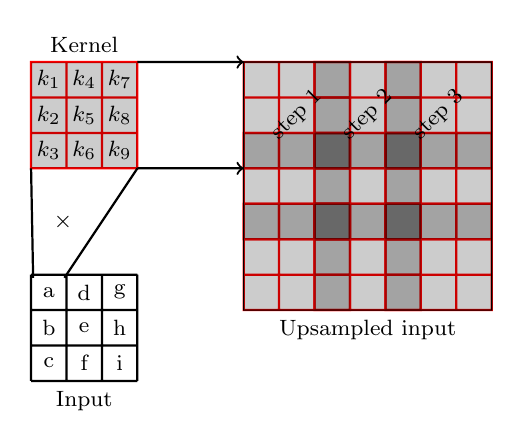
\begin{tikzpicture}

\begin{scope}[transparency group]
\begin{scope}[blend mode=multiply]
%stride 1
%kernel
\draw [thick, draw=red,fill=black!20!white, scale = .45] (-1,5) grid (2,8) rectangle (-1,5);
%kernel label
\draw [scale=.45,above] node at (0.5,8)  {\footnotesize Kernel};
%kernel components
\draw [scale=.45] node at (-0.5,7.5) {$k_1$};
\draw [scale=.45] node at (-0.5,6.5) {$k_2$};
\draw [scale=.45] node at (-0.5,5.5) {$k_3$};
\draw [scale=.45] node at (0.5,7.5)  {$k_4$};
\draw [scale=.45] node at (0.5,6.5)  {$k_5$};
\draw [scale=.45] node at (0.5,5.5)  {$k_6$};
\draw [scale=.45] node at (1.5,7.5)  {$k_7$};
\draw [scale=.45] node at (1.5,6.5)  {$k_8$};
\draw [scale=.45] node (k9) at (1.5,5.5)  {$k_9$};
%kernel on output
\draw [scale=.45] node[rotate=45] at (6.5,6.5)  {step 1};
\draw [scale=.45] node[rotate=45] at (8.5,6.5)  {step 2};
\draw [scale=.45] node[rotate=45] at (10.5,6.5)  {step 3};
%Kernel label
\draw [thick, draw=black,scale=.45] (-1,-1) grid  (2,2) node at (0.5,-1)[below] {\footnotesize Input};
% step 1 featuremap
\draw [thin, draw=black ,scale = .45] (5,1) rectangle  (12,8) node at (8.5,1) [below,text width=3cm,align= center] {\footnotesize Upsampled input};
%draw abc step 1
\draw [scale=.45] node (a) at (-.5,1.5) {a};
\draw [scale=.45] node at (-.5,0.5) {b};
\draw [scale=.45] node at (-.5,-.5) {c};
\draw [scale=.45] node at (0.5,1.5) {d};
\draw [scale=.45] node at (0.5,0.5) {e};
\draw [scale=.45] node at (0.5,-.5) {f};
\draw [scale=.45] node at (1.5,1.5) {g};
\draw [scale=.45] node at (1.5,0.5) {h};
\draw [scale=.45] node at (1.5,-.5) {i};
%draw connections
\draw [thick,scale=.45] (a.north east) -- (2,5) {};
\draw [thick,scale=.45] (a.north west) -- (-1,5){};
\draw [->,thick,scale=.45] (2,5) -- (5,5){};
\draw [->,thick,scale=.45] (2,8) -- (5,8){};
\draw [scale=.45,thick] node at (-.1,3.5) {$\mathbf{\times}$};
%draw kernel positions 
\foreach \i in {1,3,5}{
\foreach \j in {5,7,9}{
	\draw [thick, draw=red, fill=black!20!white,scale = .45] (\j,\i) grid  (\j+3,\i+3) rectangle (\j,\i);
		}
		}
\end{scope}
\end{scope}
\end{tikzpicture}

		\subcaption{Two dimensional example of the transpose of a \textbf{one} strided convolution over a \(3\times 3\) input matrix with a \(2\times 2\) kernel matrix. The equations for obtaining the components \(o\) and \(p\) of the feature map are given. The resulting feature map is a \(3\times 3\) matrix, as we upsampled the input by a factor of \(0.75\). Note that all biases are omitted for simplicity and bold symbols should help readability and do not represent vectors.}
		\label{Fig: Upsampling(a)}
	\end{subfigure}\hfill
	\begin{subfigure}{.455\textwidth}
		\centering
		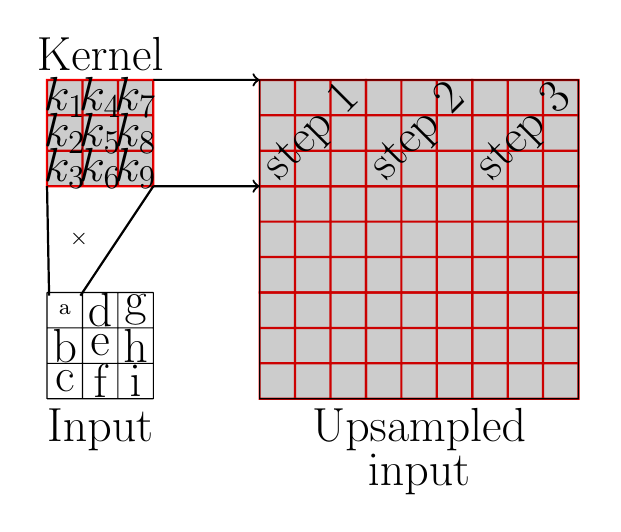
\begin{tikzpicture}
\begin{scope}[transparency group]
\begin{scope}[blend mode=multiply]

%kernel
\draw [thick, draw=red, fill=black!20!white,scale = .45] (-1,5) rectangle (2,8) grid (-1,5);
%kernel label
\draw [scale=.45,above] node at (0.5,8)  {\LARGE Kernel};
%kernel components
\draw [scale=.45] node at (-0.5,7.5) {\LARGE $k_1$};
\draw [scale=.45] node at (-0.5,6.5) {\LARGE $k_2$};
\draw [scale=.45] node at (-0.5,5.5) {\LARGE $k_3$};
\draw [scale=.45] node at (0.5,7.5)  {\LARGE $k_4$};
\draw [scale=.45] node at (0.5,6.5)  {\LARGE $k_5$};
\draw [scale=.45] node at (0.5,5.5)  {\LARGE $k_6$};
\draw [scale=.45] node at (1.5,7.5)  {\LARGE $k_7$};
\draw [scale=.45] node at (1.5,6.5)  {\LARGE $k_8$};
\draw [scale=.45] node (k9) at (1.5,5.5)  {\LARGE $k_9$};
%kernel on output
\draw [scale=.45] node [rotate=45] at (6.5,6.5)  {\LARGE step 1};
\draw [scale=.45] node [rotate=45] at (9.5,6.5)  {\LARGE step 2};
\draw [scale=.45] node [rotate=45] at (12.5,6.5) {\LARGE step 3};

% input label
\draw [thin, draw=black,scale=.45] (-1,-1) grid  (2,2) node at (0.5,-1)[below] {\LARGE Input};
% step 1 featuremap;
\draw [thin, draw=black,scale = .45] (5,-1) rectangle  (14,8) node at (9.5,-1) [below,text width=4cm,align= center] {\LARGE Upsampled input};
%draw abc
\draw [scale=.45] node (a) at (-.5,1.5) {a};
\draw [scale=.45] node at (-.5,0.5) {\LARGE b};
\draw [scale=.45] node at (-.5,-.5) {\LARGE c};
\draw [scale=.45] node at (0.5,1.5) {\LARGE d};
\draw [scale=.45] node at (0.5,0.5) {\LARGE e};
\draw [scale=.45] node at (0.5,-.5) {\LARGE f};
\draw [scale=.45] node at (1.5,1.5) {\LARGE g};
\draw [scale=.45] node at (1.5,0.5) {\LARGE h};
\draw [scale=.45] node at (1.5,-.5) {\LARGE i};
%draw connections
\draw [thick,scale=.45] (a.north east) -- (2,5) {};
\draw [thick,scale=.45] (a.north west) -- (-1,5){};
\draw [->,thick,scale=.45] (2,5) -- (5,5){};
\draw [->,thick,scale=.45] (2,8) -- (5,8){};
\draw [scale=.45,thick] node at (-.1,3.5) {$\mathbf{\times}$};
\foreach \i in {-1,2,5}
\foreach \j in {5,8,11}
	\draw [thick, draw=red, fill=black!20!white,scale = .45] (\j,\i) grid  (\j+3,\i+3) rectangle (\j,\i);

\end{scope}
\end{scope}
\end{tikzpicture}

		\subcaption{Two dimensional example of the transpose of a \textbf{one} strided convolution over over a \(2\times 2\) input matrix with a \(2\times 2\) kernel matrix. The equations for obtaining the components \(o\) and \(p\) of the feature map are given. The resulting feature map is a \(4\times 4\) matrix. Upsampling by a factor of \(0.5\) is achieved with zero padding (dashed lines). Note that all biases are omitted for simplicity and bold symbols should help readability and do not represent vectors.}
		\label{Fig: Upsampling(b)}
	\end{subfigure}
	\caption{Upsampling of the convolutions illustrated in \cref{Fig: Downsampling} using transposed convolutions. Upsampling a $3\times 3$ input matrix to a $4\times 4$ featuremap is reversing \cref{Fig: Downsampling(a)}. Upsampling a $2\times 2$ input matrix to a $4\times 4$ featuremap is reversing \cref{Fig: Downsampling(b)}.}
	\label{Fig: Upsampling}
\end{figure}
%In the discrete cross correlation in \cref{Eq. Discrete Cross Correlation} The given equation for the discrete cross correlation in two dimensions (excluding channels) illustrate the movement of a kernel over a two dimensional input. First is the so called stride of the kernel, which results in a increased down sampling with increased stride size. Considering strides of the kernel along one dimension of the input results in a shrinkage of that dimension by 
%\begin{equation}\label{Eq:Downsampling}
%	o = \frac{i -k}{s} + 1.
%\end{equation} 
%Here \(o\), \(i\), \(s\) and \(k\) are the output, input, stride and kernel size of one dimension respectively \cite{dumoulin2018guide}. Second are the so called channels, which allow convolutional layers to extract a different feature for every channel from the same input. For a two dimensional input like images this could be different features for the same location on the image, like edges and color in the RGB color space \cite{Goodfellow}. Adding strides and kernel to \cref{Eq. Discrete Cross Correlation} yields
%\begin{equation}
%	\mathsf{S}_{i,j,k} = c(\mathsf{K},\mathsf{I},s)_{i,j,k}\sum_{l,m,n}\left[\mathsf{I}_{l,(j-1)\times s+m,(k -1)\times s+n}\mathsf{K}_{i,l,m,n}\right]. \label{Eq. Cross correlation stride channel}
%\end{equation}
%The kernel \(\mathsf{K}\) is a four dimensional tensor with \(i\) indexing into the output channels of \(S\), \(l\) indexing into the input channels of \(I\), \(m\) and \(n\) indexing into the rows and colums. The input \(\mathsf{I}\) and output \(S\) are three dimensional tensors with \(j\) and \(k\) indexing into the rows and columns. Note that in \texttt{PyTorch} \cref{Eq. Cross correlation stride channel} is a so called valid cross correlation (valid convolution) \cite{bibid} meaning the kernel will only move over input units for which  all \(m\) and \(n\) are inside the rows and columns of the input. Zero padding the input can prevent the kernel from omitting corners in that case.
%\\
%For autoencoders the necessity to perform a transposition of the applied layers arises, which is straight forward for fully connected layers. Convolutional layers with strides greater than unity on the other hand  the transposition needs the kernel to be padded with zeros to realize an upsampling of the input data \cite{dumoulin2018guide}. Note that the padding of the kernel with zeros is only used to illustrate how the upsampling works. In \cref{Eq: Transposed convolution} taken from \cite{Goodfellow} multiplications with zero are omitted. The size of one dimension during upsampling can be calculated with the transposition of \cref{Eq:Downsampling}.
%\begin{equation}\label{Eq: Transposed convolution}
%	t(\mathsf{K},\mathsf{H},s)_{i,j,k} = \sum_{\substack{l,m\\s.t\\(l-1)\times s+m=j}}
%												  \sum_{\substack{n,p\\s.t\\(n-1)\times s+p=k}}
%												  \sum_q \mathsf{K}_{q,i,m,p}\mathsf{H}_{q,l,n} 
%\end{equation}


%\subsection{Autoencoders}
%Autoencoders have many hyperparameters determining their capability for compression and subsequent reconstruction. These parameters include : \textit{depth}, \textit{width of layers}, \textit{activation functions}, \textit{batch-size}, \textit{learning rate}, \textit{number of filters}, \textit{stride width}, \textit{kernel size}. Their finding is discussed in this section, for both $\hy$ and $\rare$.\\
%For the fully connected autoencoder the order of determining the hyperparameters is as follows:
%Depth $\rightarrow$ Hidden Units $\rightarrow$ Batch Size $\rightarrow$  Activation Fuctions.
%For the convolutional autoencoder the order of determining the hyperparameters is as follows:
%Depth $\rightarrow$ Channels $\rightarrow$ Batch Size $\rightarrow$ Activation Functions.
%Both models are evaluated on the course of the training. Figures showing the training process for all experiments are provided in the appendix. After training the L2-Error\cref{labellist} is evaluated on the unshuffled, complete dataset as described in \cref{Sec: Data Sampling}.\\
%Important to mention is that the difficulty of finding the right set of hyperparameters for MLPs led to an intensive search prior to the creation of this contribution. The difficulty lies in the fact that there is little systematic knowledge about how the hyperparameters interact in the model and answer to a variety of input data. Goodfellow et al. point out that with a combination of intuition, certain methods and first of all experience practitioners find hyperparameters that work well \cite{Goodfellow}. As for this thesis a list of the prior search is provided in \cref{Sec:AppendixA}. This list does not claim to cover the complete search and can by no means give enough insight to enable reproducability by another person.\\
%For this reason an insight into the methods employed to find the set of hyperparameters used in this contribution are described in the following. 
%
%The convolutional autoencoder architecture 1.1 is a composition of six convolutional and three fully conected layers, \cref{f_Conv}.
%\begin{equation}
%y_p = f_{C}^9(f_{C}^8(f_{C}^7(f_{F}^6(f_{F}^5(f_{F}^4(f_{C}^3(f_{C}^2(f_{C}^1(y_0)))))))))
%\label{f_Conv}
%\end{equation}